%% AK: TODOs:
% - TD experiment with exact behavior policy
% - Bellman backup with target network proof
% - Run weighting + stop gradient on gridworld 
% - Why is this regularization bad?
% - Formulate why the regularizer is bad? Maybe because the dot product is too high? separate out in-distribution error and OOD error
% - Some cross-validation
% - gridworlds cross-validation

\documentclass{article} % For LaTeX2e
\usepackage{iclr2022_conference,times}

% Optional math commands from https://github.com/goodfeli/dlbook_notation.
%%%%% NEW MATH DEFINITIONS %%%%%

\usepackage{amsmath,amsfonts,bm}

% Mark sections of captions for referring to divisions of figures
\newcommand{\figleft}{{\em (Left)}}
\newcommand{\figcenter}{{\em (Center)}}
\newcommand{\figright}{{\em (Right)}}
\newcommand{\figtop}{{\em (Top)}}
\newcommand{\figbottom}{{\em (Bottom)}}
\newcommand{\captiona}{{\em (a)}}
\newcommand{\captionb}{{\em (b)}}
\newcommand{\captionc}{{\em (c)}}
\newcommand{\captiond}{{\em (d)}}

% Highlight a newly defined term
\newcommand{\newterm}[1]{{\bf #1}}


% Figure reference, lower-case.
\def\figref#1{figure~\ref{#1}}
% Figure reference, capital. For start of sentence
\def\Figref#1{Figure~\ref{#1}}
\def\twofigref#1#2{figures \ref{#1} and \ref{#2}}
\def\quadfigref#1#2#3#4{figures \ref{#1}, \ref{#2}, \ref{#3} and \ref{#4}}
% Section reference, lower-case.
\def\secref#1{section~\ref{#1}}
% Section reference, capital.
\def\Secref#1{Section~\ref{#1}}
% Reference to two sections.
\def\twosecrefs#1#2{sections \ref{#1} and \ref{#2}}
% Reference to three sections.
\def\secrefs#1#2#3{sections \ref{#1}, \ref{#2} and \ref{#3}}
% Reference to an equation, lower-case.
\def\eqref#1{equation~\ref{#1}}
% Reference to an equation, upper case
\def\Eqref#1{Equation~\ref{#1}}
% A raw reference to an equation---avoid using if possible
\def\plaineqref#1{\ref{#1}}
% Reference to a chapter, lower-case.
\def\chapref#1{chapter~\ref{#1}}
% Reference to an equation, upper case.
\def\Chapref#1{Chapter~\ref{#1}}
% Reference to a range of chapters
\def\rangechapref#1#2{chapters\ref{#1}--\ref{#2}}
% Reference to an algorithm, lower-case.
\def\algref#1{algorithm~\ref{#1}}
% Reference to an algorithm, upper case.
\def\Algref#1{Algorithm~\ref{#1}}
\def\twoalgref#1#2{algorithms \ref{#1} and \ref{#2}}
\def\Twoalgref#1#2{Algorithms \ref{#1} and \ref{#2}}
% Reference to a part, lower case
\def\partref#1{part~\ref{#1}}
% Reference to a part, upper case
\def\Partref#1{Part~\ref{#1}}
\def\twopartref#1#2{parts \ref{#1} and \ref{#2}}

\def\ceil#1{\lceil #1 \rceil}
\def\floor#1{\lfloor #1 \rfloor}
\def\1{\bm{1}}
\newcommand{\train}{\mathcal{D}}
\newcommand{\valid}{\mathcal{D_{\mathrm{valid}}}}
\newcommand{\test}{\mathcal{D_{\mathrm{test}}}}

\def\eps{{\epsilon}}


% Random variables
\def\reta{{\textnormal{$\eta$}}}
\def\ra{{\textnormal{a}}}
\def\rb{{\textnormal{b}}}
\def\rc{{\textnormal{c}}}
\def\rd{{\textnormal{d}}}
\def\re{{\textnormal{e}}}
\def\rf{{\textnormal{f}}}
\def\rg{{\textnormal{g}}}
\def\rh{{\textnormal{h}}}
\def\ri{{\textnormal{i}}}
\def\rj{{\textnormal{j}}}
\def\rk{{\textnormal{k}}}
\def\rl{{\textnormal{l}}}
% rm is already a command, just don't name any random variables m
\def\rn{{\textnormal{n}}}
\def\ro{{\textnormal{o}}}
\def\rp{{\textnormal{p}}}
\def\rq{{\textnormal{q}}}
\def\rr{{\textnormal{r}}}
\def\rs{{\textnormal{s}}}
\def\rt{{\textnormal{t}}}
\def\ru{{\textnormal{u}}}
\def\rv{{\textnormal{v}}}
\def\rw{{\textnormal{w}}}
\def\rx{{\textnormal{x}}}
\def\ry{{\textnormal{y}}}
\def\rz{{\textnormal{z}}}

% Random vectors
\def\rvepsilon{{\mathbf{\epsilon}}}
\def\rvtheta{{\mathbf{\theta}}}
\def\rva{{\mathbf{a}}}
\def\rvb{{\mathbf{b}}}
\def\rvc{{\mathbf{c}}}
\def\rvd{{\mathbf{d}}}
\def\rve{{\mathbf{e}}}
\def\rvf{{\mathbf{f}}}
\def\rvg{{\mathbf{g}}}
\def\rvh{{\mathbf{h}}}
\def\rvu{{\mathbf{i}}}
\def\rvj{{\mathbf{j}}}
\def\rvk{{\mathbf{k}}}
\def\rvl{{\mathbf{l}}}
\def\rvm{{\mathbf{m}}}
\def\rvn{{\mathbf{n}}}
\def\rvo{{\mathbf{o}}}
\def\rvp{{\mathbf{p}}}
\def\rvq{{\mathbf{q}}}
\def\rvr{{\mathbf{r}}}
\def\rvs{{\mathbf{s}}}
\def\rvt{{\mathbf{t}}}
\def\rvu{{\mathbf{u}}}
\def\rvv{{\mathbf{v}}}
\def\rvw{{\mathbf{w}}}
\def\rvx{{\mathbf{x}}}
\def\rvy{{\mathbf{y}}}
\def\rvz{{\mathbf{z}}}

% Elements of random vectors
\def\erva{{\textnormal{a}}}
\def\ervb{{\textnormal{b}}}
\def\ervc{{\textnormal{c}}}
\def\ervd{{\textnormal{d}}}
\def\erve{{\textnormal{e}}}
\def\ervf{{\textnormal{f}}}
\def\ervg{{\textnormal{g}}}
\def\ervh{{\textnormal{h}}}
\def\ervi{{\textnormal{i}}}
\def\ervj{{\textnormal{j}}}
\def\ervk{{\textnormal{k}}}
\def\ervl{{\textnormal{l}}}
\def\ervm{{\textnormal{m}}}
\def\ervn{{\textnormal{n}}}
\def\ervo{{\textnormal{o}}}
\def\ervp{{\textnormal{p}}}
\def\ervq{{\textnormal{q}}}
\def\ervr{{\textnormal{r}}}
\def\ervs{{\textnormal{s}}}
\def\ervt{{\textnormal{t}}}
\def\ervu{{\textnormal{u}}}
\def\ervv{{\textnormal{v}}}
\def\ervw{{\textnormal{w}}}
\def\ervx{{\textnormal{x}}}
\def\ervy{{\textnormal{y}}}
\def\ervz{{\textnormal{z}}}

% Random matrices
\def\rmA{{\mathbf{A}}}
\def\rmB{{\mathbf{B}}}
\def\rmC{{\mathbf{C}}}
\def\rmD{{\mathbf{D}}}
\def\rmE{{\mathbf{E}}}
\def\rmF{{\mathbf{F}}}
\def\rmG{{\mathbf{G}}}
\def\rmH{{\mathbf{H}}}
\def\rmI{{\mathbf{I}}}
\def\rmJ{{\mathbf{J}}}
\def\rmK{{\mathbf{K}}}
\def\rmL{{\mathbf{L}}}
\def\rmM{{\mathbf{M}}}
\def\rmN{{\mathbf{N}}}
\def\rmO{{\mathbf{O}}}
\def\rmP{{\mathbf{P}}}
\def\rmQ{{\mathbf{Q}}}
\def\rmR{{\mathbf{R}}}
\def\rmS{{\mathbf{S}}}
\def\rmT{{\mathbf{T}}}
\def\rmU{{\mathbf{U}}}
\def\rmV{{\mathbf{V}}}
\def\rmW{{\mathbf{W}}}
\def\rmX{{\mathbf{X}}}
\def\rmY{{\mathbf{Y}}}
\def\rmZ{{\mathbf{Z}}}

% Elements of random matrices
\def\ermA{{\textnormal{A}}}
\def\ermB{{\textnormal{B}}}
\def\ermC{{\textnormal{C}}}
\def\ermD{{\textnormal{D}}}
\def\ermE{{\textnormal{E}}}
\def\ermF{{\textnormal{F}}}
\def\ermG{{\textnormal{G}}}
\def\ermH{{\textnormal{H}}}
\def\ermI{{\textnormal{I}}}
\def\ermJ{{\textnormal{J}}}
\def\ermK{{\textnormal{K}}}
\def\ermL{{\textnormal{L}}}
\def\ermM{{\textnormal{M}}}
\def\ermN{{\textnormal{N}}}
\def\ermO{{\textnormal{O}}}
\def\ermP{{\textnormal{P}}}
\def\ermQ{{\textnormal{Q}}}
\def\ermR{{\textnormal{R}}}
\def\ermS{{\textnormal{S}}}
\def\ermT{{\textnormal{T}}}
\def\ermU{{\textnormal{U}}}
\def\ermV{{\textnormal{V}}}
\def\ermW{{\textnormal{W}}}
\def\ermX{{\textnormal{X}}}
\def\ermY{{\textnormal{Y}}}
\def\ermZ{{\textnormal{Z}}}

% Vectors
\def\vzero{{\bm{0}}}
\def\vone{{\bm{1}}}
\def\vmu{{\bm{\mu}}}
\def\vtheta{{\bm{\theta}}}
\def\va{{\bm{a}}}
\def\vb{{\bm{b}}}
\def\vc{{\bm{c}}}
\def\vd{{\bm{d}}}
\def\ve{{\bm{e}}}
\def\vf{{\bm{f}}}
\def\vg{{\bm{g}}}
\def\vh{{\bm{h}}}
\def\vi{{\bm{i}}}
\def\vj{{\bm{j}}}
\def\vk{{\bm{k}}}
\def\vl{{\bm{l}}}
\def\vm{{\bm{m}}}
\def\vn{{\bm{n}}}
\def\vo{{\bm{o}}}
\def\vp{{\bm{p}}}
\def\vq{{\bm{q}}}
\def\vr{{\bm{r}}}
\def\vs{{\bm{s}}}
\def\vt{{\bm{t}}}
\def\vu{{\bm{u}}}
\def\vv{{\bm{v}}}
\def\vw{{\bm{w}}}
\def\vx{{\bm{x}}}
\def\vy{{\bm{y}}}
\def\vz{{\bm{z}}}

% Elements of vectors
\def\evalpha{{\alpha}}
\def\evbeta{{\beta}}
\def\evepsilon{{\epsilon}}
\def\evlambda{{\lambda}}
\def\evomega{{\omega}}
\def\evmu{{\mu}}
\def\evpsi{{\psi}}
\def\evsigma{{\sigma}}
\def\evtheta{{\theta}}
\def\eva{{a}}
\def\evb{{b}}
\def\evc{{c}}
\def\evd{{d}}
\def\eve{{e}}
\def\evf{{f}}
\def\evg{{g}}
\def\evh{{h}}
\def\evi{{i}}
\def\evj{{j}}
\def\evk{{k}}
\def\evl{{l}}
\def\evm{{m}}
\def\evn{{n}}
\def\evo{{o}}
\def\evp{{p}}
\def\evq{{q}}
\def\evr{{r}}
\def\evs{{s}}
\def\evt{{t}}
\def\evu{{u}}
\def\evv{{v}}
\def\evw{{w}}
\def\evx{{x}}
\def\evy{{y}}
\def\evz{{z}}

% Matrix
\def\mA{{\bm{A}}}
\def\mB{{\bm{B}}}
\def\mC{{\bm{C}}}
\def\mD{{\bm{D}}}
\def\mE{{\bm{E}}}
\def\mF{{\bm{F}}}
\def\mG{{\bm{G}}}
\def\mH{{\bm{H}}}
\def\mI{{\bm{I}}}
\def\mJ{{\bm{J}}}
\def\mK{{\bm{K}}}
\def\mL{{\bm{L}}}
\def\mM{{\bm{M}}}
\def\mN{{\bm{N}}}
\def\mO{{\bm{O}}}
\def\mP{{\bm{P}}}
\def\mQ{{\bm{Q}}}
\def\mR{{\bm{R}}}
\def\mS{{\bm{S}}}
\def\mT{{\bm{T}}}
\def\mU{{\bm{U}}}
\def\mV{{\bm{V}}}
\def\mW{{\bm{W}}}
\def\mX{{\bm{X}}}
\def\mY{{\bm{Y}}}
\def\mZ{{\bm{Z}}}
\def\mBeta{{\bm{\beta}}}
\def\mPhi{{\bm{\Phi}}}
\def\mLambda{{\bm{\Lambda}}}
\def\mSigma{{\bm{\Sigma}}}

% Tensor
\DeclareMathAlphabet{\mathsfit}{\encodingdefault}{\sfdefault}{m}{sl}
\SetMathAlphabet{\mathsfit}{bold}{\encodingdefault}{\sfdefault}{bx}{n}
\newcommand{\tens}[1]{\bm{\mathsfit{#1}}}
\def\tA{{\tens{A}}}
\def\tB{{\tens{B}}}
\def\tC{{\tens{C}}}
\def\tD{{\tens{D}}}
\def\tE{{\tens{E}}}
\def\tF{{\tens{F}}}
\def\tG{{\tens{G}}}
\def\tH{{\tens{H}}}
\def\tI{{\tens{I}}}
\def\tJ{{\tens{J}}}
\def\tK{{\tens{K}}}
\def\tL{{\tens{L}}}
\def\tM{{\tens{M}}}
\def\tN{{\tens{N}}}
\def\tO{{\tens{O}}}
\def\tP{{\tens{P}}}
\def\tQ{{\tens{Q}}}
\def\tR{{\tens{R}}}
\def\tS{{\tens{S}}}
\def\tT{{\tens{T}}}
\def\tU{{\tens{U}}}
\def\tV{{\tens{V}}}
\def\tW{{\tens{W}}}
\def\tX{{\tens{X}}}
\def\tY{{\tens{Y}}}
\def\tZ{{\tens{Z}}}


% Graph
\def\gA{{\mathcal{A}}}
\def\gB{{\mathcal{B}}}
\def\gC{{\mathcal{C}}}
\def\gD{{\mathcal{D}}}
\def\gE{{\mathcal{E}}}
\def\gF{{\mathcal{F}}}
\def\gG{{\mathcal{G}}}
\def\gH{{\mathcal{H}}}
\def\gI{{\mathcal{I}}}
\def\gJ{{\mathcal{J}}}
\def\gK{{\mathcal{K}}}
\def\gL{{\mathcal{L}}}
\def\gM{{\mathcal{M}}}
\def\gN{{\mathcal{N}}}
\def\gO{{\mathcal{O}}}
\def\gP{{\mathcal{P}}}
\def\gQ{{\mathcal{Q}}}
\def\gR{{\mathcal{R}}}
\def\gS{{\mathcal{S}}}
\def\gT{{\mathcal{T}}}
\def\gU{{\mathcal{U}}}
\def\gV{{\mathcal{V}}}
\def\gW{{\mathcal{W}}}
\def\gX{{\mathcal{X}}}
\def\gY{{\mathcal{Y}}}
\def\gZ{{\mathcal{Z}}}

% Sets
\def\sA{{\mathbb{A}}}
\def\sB{{\mathbb{B}}}
\def\sC{{\mathbb{C}}}
\def\sD{{\mathbb{D}}}
% Don't use a set called E, because this would be the same as our symbol
% for expectation.
\def\sF{{\mathbb{F}}}
\def\sG{{\mathbb{G}}}
\def\sH{{\mathbb{H}}}
\def\sI{{\mathbb{I}}}
\def\sJ{{\mathbb{J}}}
\def\sK{{\mathbb{K}}}
\def\sL{{\mathbb{L}}}
\def\sM{{\mathbb{M}}}
\def\sN{{\mathbb{N}}}
\def\sO{{\mathbb{O}}}
\def\sP{{\mathbb{P}}}
\def\sQ{{\mathbb{Q}}}
\def\sR{{\mathbb{R}}}
\def\sS{{\mathbb{S}}}
\def\sT{{\mathbb{T}}}
\def\sU{{\mathbb{U}}}
\def\sV{{\mathbb{V}}}
\def\sW{{\mathbb{W}}}
\def\sX{{\mathbb{X}}}
\def\sY{{\mathbb{Y}}}
\def\sZ{{\mathbb{Z}}}

% Entries of a matrix
\def\emLambda{{\Lambda}}
\def\emA{{A}}
\def\emB{{B}}
\def\emC{{C}}
\def\emD{{D}}
\def\emE{{E}}
\def\emF{{F}}
\def\emG{{G}}
\def\emH{{H}}
\def\emI{{I}}
\def\emJ{{J}}
\def\emK{{K}}
\def\emL{{L}}
\def\emM{{M}}
\def\emN{{N}}
\def\emO{{O}}
\def\emP{{P}}
\def\emQ{{Q}}
\def\emR{{R}}
\def\emS{{S}}
\def\emT{{T}}
\def\emU{{U}}
\def\emV{{V}}
\def\emW{{W}}
\def\emX{{X}}
\def\emY{{Y}}
\def\emZ{{Z}}
\def\emSigma{{\Sigma}}

% entries of a tensor
% Same font as tensor, without \bm wrapper
\newcommand{\etens}[1]{\mathsfit{#1}}
\def\etLambda{{\etens{\Lambda}}}
\def\etA{{\etens{A}}}
\def\etB{{\etens{B}}}
\def\etC{{\etens{C}}}
\def\etD{{\etens{D}}}
\def\etE{{\etens{E}}}
\def\etF{{\etens{F}}}
\def\etG{{\etens{G}}}
\def\etH{{\etens{H}}}
\def\etI{{\etens{I}}}
\def\etJ{{\etens{J}}}
\def\etK{{\etens{K}}}
\def\etL{{\etens{L}}}
\def\etM{{\etens{M}}}
\def\etN{{\etens{N}}}
\def\etO{{\etens{O}}}
\def\etP{{\etens{P}}}
\def\etQ{{\etens{Q}}}
\def\etR{{\etens{R}}}
\def\etS{{\etens{S}}}
\def\etT{{\etens{T}}}
\def\etU{{\etens{U}}}
\def\etV{{\etens{V}}}
\def\etW{{\etens{W}}}
\def\etX{{\etens{X}}}
\def\etY{{\etens{Y}}}
\def\etZ{{\etens{Z}}}

% The true underlying data generating distribution
\newcommand{\pdata}{p_{\rm{data}}}
% The empirical distribution defined by the training set
\newcommand{\ptrain}{\hat{p}_{\rm{data}}}
\newcommand{\Ptrain}{\hat{P}_{\rm{data}}}
% The model distribution
\newcommand{\pmodel}{p_{\rm{model}}}
\newcommand{\Pmodel}{P_{\rm{model}}}
\newcommand{\ptildemodel}{\tilde{p}_{\rm{model}}}
% Stochastic autoencoder distributions
\newcommand{\pencode}{p_{\rm{encoder}}}
\newcommand{\pdecode}{p_{\rm{decoder}}}
\newcommand{\precons}{p_{\rm{reconstruct}}}

\newcommand{\laplace}{\mathrm{Laplace}} % Laplace distribution

\newcommand{\E}{\mathbb{E}}
\newcommand{\Ls}{\mathcal{L}}
\newcommand{\R}{\mathbb{R}}
\newcommand{\emp}{\tilde{p}}
\newcommand{\lr}{\alpha}
\newcommand{\reg}{\lambda}
\newcommand{\rect}{\mathrm{rectifier}}
\newcommand{\softmax}{\mathrm{softmax}}
\newcommand{\sigmoid}{\sigma}
\newcommand{\softplus}{\zeta}
\newcommand{\KL}{D_{\mathrm{KL}}}
\newcommand{\Var}{\mathrm{Var}}
\newcommand{\standarderror}{\mathrm{SE}}
\newcommand{\Cov}{\mathrm{Cov}}
% Wolfram Mathworld says $L^2$ is for function spaces and $\ell^2$ is for vectors
% But then they seem to use $L^2$ for vectors throughout the site, and so does
% wikipedia.
\newcommand{\normlzero}{L^0}
\newcommand{\normlone}{L^1}
\newcommand{\normltwo}{L^2}
\newcommand{\normlp}{L^p}
\newcommand{\normmax}{L^\infty}
\newcommand{\gradlossktj}{\frac{\partial L_{k+1}(\bW_{N:1}(k, t))}{\partial \bW_j(k, t)}}

\newcommand{\parents}{Pa} % See usage in notation.tex. Chosen to match Daphne's book.

\DeclareMathOperator*{\argmax}{arg\,max}
\DeclareMathOperator*{\argmin}{arg\,min}

\DeclareMathOperator{\sign}{sign}
\DeclareMathOperator{\Tr}{Tr}
\let\ab\allowbreak


\usepackage[utf8]{inputenc} % allow utf-8 input
\usepackage[T1]{fontenc}    % use 8-bit T1 fonts
\usepackage{url}            % simple URL typesetting
\usepackage{booktabs}       % professional-quality tables
\usepackage{amsfonts}       % blackboard math symbols
\usepackage{nicefrac}       % compact symbols for 1/2, etc.
\usepackage{microtype}      % microtypography
\usepackage{xcolor}         % colors
\usepackage{fleqn, tabularx}
\usepackage{multirow}
\usepackage{mathtools}
\usepackage[export]{adjustbox}
\usepackage{amsmath}
\usepackage{amssymb}
\usepackage{colortbl}
\usepackage{wrapfig}
\usepackage{algorithm}
\usepackage[noend]{algorithmic}
\usepackage{xcolor}
\usepackage{caption}
\usepackage{mathrsfs}
\usepackage{chngcntr}


\usepackage[colorlinks=true,allcolors=blue]{hyperref}

\usepackage{amsmath,amssymb,amsthm}
\usepackage{algorithm,algorithmic}
\usepackage{mathtools}
\usepackage[skins,theorems]{tcolorbox}

%% editing comment
\newcommand{\cmt}[1]{{\footnotesize\textcolor{red}{#1}}}
\newcommand{\cmto}[1]{{\footnotesize\textcolor{orange}{#1}}}
\newcommand{\note}[1]{\cmt{Note: #1}}
\newcommand{\todo}[1]{\cmt{TO-DO: #1}}
\newcommand{\question}[1]{\cmto{Question: #1}}
\newcommand{\sergey}[1]{{\footnotesize\textcolor{blue}{Sergey: #1}}}
\newcommand{\ak}[1]{{\textcolor{black}{#1}}}
\newcommand{\edits}[1]{\textcolor{blue}{#1}}
\newcommand{\editsred}[1]{\textcolor{red}{#1}}
\newcommand{\editsp}[1]{\textcolor{purple}{#1}}
\newcommand{\editsv}[1]{\textcolor{magenta}{#1}}


\newcommand{\methodname}{Cal-QL}
\newcommand{\aliasingproblemname}{bootstrapping aliasing}
\newcommand{\Aliasingproblemname}{Bootstrapping aliasing}
\newcommand{\AliasingProblemName}{Bootstrapping Aliasing}
\newcommand{\simnorm}{\mathrm{sim}_{\mathrm{n}}^\pi}
\newcommand{\simunnorm}{\mathrm{sim}_{\mathrm{u}}^\pi}

%% abbreviations
\newcommand{\x}{\mathbf{x}}
\newcommand{\z}{\mathbf{z}}
\newcommand{\y}{\mathbf{y}}
\newcommand{\w}{\mathbf{w}}
\newcommand{\data}{\mathcal{D}}

\newcommand{\etal}{{et~al.}\ }
\newcommand{\eg}{e.g.\ }
\newcommand{\ie}{i.e.\ }
\newcommand{\nth}{\text{th}}
\newcommand{\pr}{^\prime}
\newcommand{\tr}{^\mathrm{T}}
\newcommand{\inv}{^{-1}}
\newcommand{\pinv}{^{\dagger}}
\newcommand{\real}{\mathbb{R}}
\newcommand{\gauss}{\mathcal{N}}
\newcommand{\norm}[1]{\left|#1\right|}
\newcommand{\trace}{\text{tr}}

%% specifics for the paper
\newcommand{\reward}{r}
\newcommand{\policy}{\pi}
\newcommand{\mdp}{\mathcal{M}}
\newcommand{\states}{\mathcal{S}}
\newcommand{\actions}{\mathcal{A}}
\newcommand{\observations}{\mathcal{O}}
\newcommand{\transitions}{T}
\newcommand{\initstate}{d_0}
\newcommand{\freq}{d}
\newcommand{\obsfunc}{E}
\newcommand{\initial}{\mathcal{I}}
\newcommand{\horizon}{H}
\newcommand{\rewardevent}{R}
\newcommand{\probr}{p_\rewardevent}
\newcommand{\metareward}{\bar{\reward}}
\newcommand{\discount}{\gamma}
\newcommand{\behavior}{{\pi_\beta}}
\newcommand{\bellman}{\mathcal{B}}
\newcommand{\qparams}{\phi}
\newcommand{\qparamset}{\Phi}
\newcommand{\qset}{\mathcal{Q}}
\newcommand{\batch}{B}
\newcommand{\qfeat}{\mathbf{f}}
\newcommand{\Qfeat}{\mathbf{F}}
\newcommand{\hatbehavior}{\hat{\pi}_\beta}

\newcommand{\traj}{\tau}

\newcommand{\pihi}{\pi^{\text{hi}}}
\newcommand{\pilo}{\pi^{\text{lo}}}
\newcommand{\ah}{\mathbf{w}}

\newcommand{\proj}{\Pi}

\newcommand{\loss}{\mathcal{L}}
\newcommand{\eye}{\mathbf{I}}

\newcommand{\model}{\hat{p}}
\newcommand{\mhat}{\hat{\mathcal{M}}}
\newcommand{\mdphat}{\widehat{\mathcal{M}}}
\newcommand{\mdpbar}{\overline{\mathcal{M}}}

\newcommand{\pimix}{\pi_{\text{mix}}}

\newcommand{\pib}{\bar{\pi}}
\newcommand{\epspi}{\epsilon_{\pi}}
\newcommand{\epsmodel}{\epsilon_{m}}

\newcommand{\return}{\mathcal{R}}

%% math
\newcommand{\cY}{\mathcal{Y}}
\newcommand{\cX}{\mathcal{X}}
\newcommand{\en}{\mathcal{E}}
\newcommand{\bu}{\mathbf{u}}
\newcommand{\bv}{\mathbf{v}}
\newcommand{\be}{\mathbf{e}}
\newcommand{\by}{\mathbf{y}}
\newcommand{\bx}{\mathbf{x}}
\newcommand{\bz}{\mathbf{z}}
\newcommand{\bw}{\mathbf{w}}
\newcommand{\bo}{\mathbf{o}}
\newcommand{\bs}{\mathbf{s}}
\newcommand{\ba}{\mathbf{a}}
\newcommand{\bM}{\mathbf{M}}
\newcommand{\ot}{\bo_t}
\newcommand{\st}{\bs_t}
\newcommand{\at}{\ba_t}
\newcommand{\op}{\mathcal{O}}
\newcommand{\opt}{\op_t}
\newcommand{\kl}{D_\text{KL}}
\newcommand{\tv}{D_\text{TV}}
\newcommand{\ent}{\mathcal{H}}
\newcommand{\bG}{\mathbf{G}}
\newcommand{\byk}{\mathbf{y_k}}
\newcommand{\bI}{\mathbf{I}}
\newcommand{\bg}{\mathbf{g}}
\newcommand{\bV}{\mathbf{V}}
\newcommand{\bD}{\mathbf{D}}
\newcommand{\bR}{\mathbf{R}}
\newcommand{\bQ}{\mathbf{Q}}
\newcommand{\bA}{\mathbf{A}}
\newcommand{\bN}{\mathbf{N}}
\newcommand{\bS}{\mathbf{S}}
\newcommand{\bW}{\mathbf{W}}
\newcommand{\bU}{\mathbf{U}}
\newcommand{\bO}{\mathbf{O}}

\newcommand{\bzhi}{\bz^\text{hi}}

\newcommand{\expected}{\mathbb{E}}
\newcommand{\E}{\mathbb{E}}
\newcommand{\srank}{\text{srank}}
\newcommand{\rank}{\text{rank}}
\newcommand{\deepnet}{\bW_N(k, t) \bW_\phi(k, t)}
\newcommand{\features}{\bW_\phi(k, t)}
\newcommand{\stateactioni}{[\bs_i; \ba_i]}
\newcommand{\diag}{\text{\textbf{diag}}}

\def\thetaP{\theta^{\prime}}
\def\cf{\emph{c.f.}\ }
\def\vs{\emph{vs}.\ }
\def\etc{\emph{etc.}\ }
\def\Eqref#1{Equation~\ref{#1}}

\newenvironment{repeatedthm}[1]{\@begintheorem{#1}{\unskip}}{\@endtheorem}
\newcommand{\algname}{COMBO\xspace}

\newtheorem{theorem}{Theorem}[section]
\newtheorem{sketchtheorem}{Sketch Theorem}[section]
\newtheorem{lemma}[theorem]{Lemma}
\newtheorem{corollary}[theorem]{Corollary}
\newtheorem{proposition}[theorem]{Proposition}
\newtheorem{definition}[theorem]{Definition}
\newtheorem{conjecture}[theorem]{Conjecture}
\newtheorem{problem}[theorem]{Problem}
\newtheorem{formulation}[theorem]{Formulation}
\newtheorem{claim}[theorem]{Claim}
\newtheorem{remark}[theorem]{Remark}
\newtheorem{example}[theorem]{Example}
\newtheorem{assumption}[theorem]{Assumption}
\newtheorem{exercise}[theorem]{Exercise}


\newcommand{\indep}{\rotatebox[origin=c]{90}{$\models$}}

\renewcommand{\mathbf}{\boldsymbol}

\newcommand{\conv}{\circledast}
\newcommand{\mb}{\mathbf}
\newcommand{\mc}{\mathcal}
\newcommand{\mf}{\mathfrak}
\newcommand{\md}{\mathds}
\newcommand{\bb}{\mathbb}
\newcommand{\msf}{\mathsf}
\newcommand{\mcr}{\mathscr}
\newcommand{\magnitude}[1]{ \left| #1 \right| }
\newcommand{\set}[1]{\left\{ #1 \right\}}
\newcommand{\condset}[2]{ \left\{ #1 \;\middle|\; #2 \right\} }


\newcommand{\reals}{\bb R}
\newcommand{\proj}{\mathrm{proj}}

\newcommand{\eps}{\varepsilon}
\newcommand{\R}{\reals}
\newcommand{\Cp}{\bb C}
\newcommand{\Z}{\bb Z}
\newcommand{\N}{\bb N}
\newcommand{\Sp}{\bb S}
\newcommand{\Ba}{\bb B}
\newcommand{\indicator}[1]{\mathbbm 1\left\{#1\right\}}
\renewcommand{\P}{\mathbb{P}}
\newcommand{\rvline}{\hspace*{-\arraycolsep}\vline\hspace*{-\arraycolsep}}
\makeatletter
\def\Ddots{\mathinner{\mkern1mu\raise\p@
\vbox{\kern7\p@\hbox{.}}\mkern2mu
\raise4\p@\hbox{.}\mkern2mu\raise7\p@\hbox{.}\mkern1mu}}
\makeatother
% to declare new operator
% \DeclareMathOperator{\xxx}{xxx}

%% Other definitions

\newcommand{\event}{\mc E}

\newcommand{\e}{\mathrm{e}}
\newcommand{\im}{\mathrm{i}}
\newcommand{\rconcave}{r_\fgecap}
\newcommand{\Lconcave}{\mc L^\fgecap}
\newcommand{\rconvex}{r_\fgecup}
\newcommand{\Rconvex}{R_\fgecup}
\newcommand{\Lconvex}{\mc L^\fgecup}

\newcommand{\wh}{\widehat}
\newcommand{\wt}{\widetilde}
\newcommand{\ol}{\overline}


\newcommand{\betaconcave}{\beta_\fgecap}
\newcommand{\betagrad}{\beta_{\mathrm{grad}}}

\newcommand{\norm}[2]{\left\| #1 \right\|_{#2}}
\newcommand{\abs}[1]{\left| #1 \right|}
\newcommand{\row}[1]{\text{row}\left( #1 \right)}
\newcommand{\innerprod}[2]{\left\langle #1,  #2 \right\rangle}
\newcommand{\prob}[1]{\bb P\left[ #1 \right]}
\newcommand{\expect}[1]{\bb E\left[ #1 \right]}
\newcommand{\function}[2]{#1 \left(#2\right}
\newcommand{\integral}[4]{\int_{#1}^{#2}\; #3\; #4}
\newcommand{\paren}[1]{\left( #1 \right)}
\newcommand{\brac}[1]{\left[ #1 \right]}
\newcommand{\Brac}[1]{\left\{ #1 \right\}}

% Adding new defs here
\newcommand{\moff}{m_\mr{off}}
\newcommand{\mon}{m_\mr{on}}
\newcommand{\EmpiricalOffline}{\wh{\bb E}_{\mc D^\nu_h}}
\newcommand{\EmpiricalOnline}{\wh{\bb E}_{\mc D^\tau_h}}
\newcommand{\Deltaoff}{\Delta_\mr{off}}
\newcommand{\Deltaon}{\Delta_\mr{on}}
\newcommand{\Vmax}{V_{\max}}
\newcommand{\regret}{\mr{Reg}}
\newcommand{\regreton}{\mr{Sub}_{\mr {on}}}
\newcommand{\regretoff}{\mr{Sub}_{\mr {off}}}
\newcommand{\Doff}{\mc D_\mr{off}}
\newcommand{\Don}{\mc D_\mr{on}}
\newcommand{\piref}{\pi_\mr{ref}}

\newcommand{\nt}[1]{{\color{purple}{\bf [Next: #1]}}}
\newcommand{\here}{{\color{purple}{\bf [Writing here]}}}
% \newcommand{\todo}{{\color{purple}{\bf [TODO]}}}
\newcommand{\sz}[1]{{\color{blue}{\bf [Simon: #1]}}}
% \newcommand{\note}[1]{{\color{red}{\bf [note: #1]}}}
\newcommand{\mr}{\mathrm}
\newcommand{\sym}{\mathrm{Sym}}
\newcommand{\sks}{\mathrm{Skew}}
\newcommand{\inprod}[2]{\langle#1,#2\rangle}
\newcommand{\parans}[1]{\left(#1\right}
\newcommand{\clip}{\msf{clipped}}
\newcommand{\beha}{\msf b}
\numberwithin{equation}{section}

% \def \endprf{\hfill {\vrule height6pt width6pt depth0pt}\medskip}

\newcommand{\cdsmethodname}{CDS}
\newcommand{\udsmethodname}{UDS}
\newcommand{\ptrmethodname}{PTR~}
\newcommand{\primemethodname}{PRIME~}
\newcommand{\arxiv}[1] {{\color{black} #1}}

% \newenvironment{proof}{\noindent {\bf Proof} }{\endprf\par}

% \newcommand{\qed}{{\unskip\nobreak\hfil\penalty50\hskip2em\vadjust{}
%            \nobreak\hfil$\Box$\parfillskip=0pt\finalhyphendemerits=0\par}}


\newcommand\myworries[1]{\textcolor{red}{#1}}
\newcommand\running[1]{\textcolor{blue}{#1}}

\newcommand{\benchl}[1]{{\scriptsize\textsf{#1}}\normalsize\xspace}
\newcommand{\bench}[1]{{\fontsize{8.5}{10}\selectfont\textsf{#1}}\normalsize\xspace}
\newcommand{\code}[1]{{\fontsize{8.5}{1}\selectfont{\tt #1}}\xspace}
\newcommand{\codebold}[1]{{\fontsize{8.5}{1}\selectfont{\tt \textbf{#1}}}\xspace}
\newcommand{\xx}[1]{\textcolor{black}{#1}}
\newcommand{\xxs}[1]{\textcolor{black}{\scriptsize\textsf{#1}}}
\newcommand{\supertiny}[1]{\fontsize{5}{4}\selectfont{#1}}
\newcommand{\xxred}[1]{\textcolor{red}{\textsf{#1}}}
% \DeclareMathOperator{\EX}{\mathbb{\hat{E}}}% expected value
% \makeatletter
% \newcommand\footnoteref[1]{\protected@xdef\@thefnmark{\ref{#1}}\@footnotemark}
% \makeatother
% \usepackage{scrextend}

% \deffootnote[1em]{1em}{1em}{\textsuperscript{\thefootnotemark}\,}
% \newcolumntype{P}[1]{>{\centering\arraybackslash}p{#1}}
% \newcommand\mycommfont[1]{\footnotesize\ttfamily\textcolor{blue}{#1}}

\newcommand\aviral[1]{\textcolor{red}{aviralkumar@: #1}}
\newcommand\ayazdan[1]{\textcolor{red}{ayazdan@: #1}}
\newcommand\sv[1]{\textcolor{red}{SV@: #1}}
\newcommand\fix[1]{\textcolor{green}{#1}}

\newcommand{\round}[1]{\ensuremath{\lfloor#1\rceil}}

\newcommand{\tgray}[1]{\colorbox{lightgray}{\textbf{#1}}}
\newcommand{\finalcheck}[1]{\textcolor{green}{#1}}

\newcommand{\review}[1]{#1}

\newcommand{\niparagraph}[1]{\vspace{2pt}\noindent\textbf{#1}}


\tcbset{
  aibox/.style={
    width=\textwidth,
    top=0pt, bottom=0pt, left=5pt, right=5pt,
    colback=black!6!white,
    colframe=black,
    colbacktitle=brown,
    enhanced,
    center,
    attach boxed title to top left={yshift=-0.1in,xshift=0.15in},
    boxed title style={boxrule=0pt,colframe=black,},
  }
}
\newtcolorbox{AIbox}[2][]{aibox,title=#2,#1}

\newtheorem{claim}{Claim}
\newtheorem{assumption}{Assumption}
\newtheorem{theorem}{Theorem}[section]
\newtheorem{lemma}[theorem]{Lemma}
\newtheorem{corollary}[theorem]{Corollary}
\newtheorem{remark}[theorem]{Remark}
\newtheorem{proposition}[theorem]{Proposition}
\newtheorem{definition}{Definition}
\renewcommand\theassumption{A\arabic{assumption}}

% hyperref makes hyperlinks in the resulting PDF.
% If your build breaks (sometimes temporarily if a hyperlink spans a page)
% please comment out the following usepackage line and replace
% \usepackage{icml2021} with \usepackage[nohyperref]{icml2021} above.
% \usepackage{hyperref}

% Attempt to make hyperref and algorithmic work together better:
\newcommand{\theHalgorithm}{\arabic{algorithm}}

\newcommand{\rebuttal}[1]{#1}


\iclrfinalcopy


\title{DR3: Value-Based \underline{D}eep \underline{R}einforcement\\ Learning \underline{R}equires Explicit \underline{R}egularization}
%%SL.9.17: Generally this title could work, though it might be a little weird if the title is METHODNAME: [some statement that doesn't pertain to the method] (i.e., the rest of the title sounds like it's an analysis paper, so it's somehow jarring to see a method name in there...). But maybe that's OK, because the paper *is* about both an analysis and a method, so in that sense though it might be jarring, it actually sets the right expectation. As a nitpick, it's also a tiny bit awkward to have "Learning" split over two lines (but better than having a three-line title). You could go with "Value-Based Deep RL Requires Explicit Regularization" (it's a bit informal to use an acronym, but it does make the title shorter)

% Authors must not appear in the submitted version. They should be hidden
% as long as the \iclrfinalcopy macro remains commented out below.
% Non-anonymous submissions will be rejected without review.

\author{
 \quad \quad \quad \quad \quad \quad \quad \quad \quad \quad \quad {Aviral Kumar$^{1, 2}$~~~~ Rishabh Agarwal$^{2, 3}$} \vspace{0.05cm}\\
\quad \quad \quad \quad \quad \quad {\textbf{Tengyu Ma$^{4}$~~~ Aaron Courville$^{3}$~~~ George Tucker$^{2}$~~~ Sergey Levine$^{1,2}$}} \vspace{0.1cm}\\
\quad \quad \quad \quad \quad ~~~ {$^1$ UC Berkeley~~~ $^2$ Google Research~~~ $^3$ MILA~~~ $^4$ Stanford University} \vspace{0.05cm}\\
\quad \quad \quad \quad \quad \quad \quad \quad \quad \quad \quad \quad \quad \quad \quad {\texttt{aviralk@berkeley.edu}}
}

% The \author macro works with any number of authors. There are two commands
% used to separate the names and addresses of multiple authors: \And and \AND.
%
% Using \And between authors leaves it to \LaTeX{} to determine where to break
% the lines. Using \AND forces a linebreak at that point. So, if \LaTeX{}
% puts 3 of 4 authors names on the first line, and the last on the second
% line, try using \AND instead of \And before the third author name.

\newcommand{\fix}{\marginpar{FIX}}
\newcommand{\new}{\marginpar{NEW}}

\iclrfinalcopy % Uncomment for camera-ready version, but NOT for submission.
\begin{document}

\part*{\Large{Significant Publication 2: \\ DR3: Value-Based Deep Reinforcement Learning Requires Explicit Regularization}}

\section*{Author List} Aviral Kumar, Rishabh Agarwal, Tengyu Ma, Aaron Courville, George Tucker, Sergey Levine

\section*{Significance of the Paper} 

{\textbf{Summary.}} This paper aims to understand the reasons behind the``capacity loss'' phenomenon that appears with offline reinforcement learning (RL) methods based on Q-learning instantiated with deep neural network function approximators. The key insight in this paper is the implicit regularization effect of gradient descent with over-parameterized models, which is regarded as the reason behind effective performance of supervised learning, actually inhibits effective use of model capacity with offline RL loss functions. This in turn inhibits effective generalization abilities of these methods. In this paper, I present a method called DR3, which aims to cancel the component of the implicit regularizer that encourages capacity loss.

\textbf{Significance.} This paper presents a starting point for understanding the impact of deep neural network function approximators on offline RL. While traditional analysis of offline RL methods (and more generally all of RL methods) with function approximation operates in the linear setting or with no assumptions on the function class, neither of them represent the conditions under which practical algorithms operate. Therefore, it is necessary to understand and build on assumptions that are closer to reality to be able to build RL algorithms that are easy to use and reliable. I believe that this work of mine presents a starting point for such analyses to build on and shows how insights from theoretical analysis can give rise to simple regularization procedures that work well in practice. 

In practice, my follow-up work (\url{https://arxiv.org/abs/2211.15144}) shows that by leveraging DR3 in conjunction with CQL (my significant publication 1), we are able to make significant progress towards scaling up offline reinforcement learning to use large datasets of size $\sim$2 billion in conjunction with effective use of capacity of large networks ($\sim$80 million parameters) for the first time (to the best of our knowledge).   

\textbf{Impact.} This work was featured as a spotlight presentation at ICLR 2022. This work was features via a oral presentations at three workshops 
 as shown below (which includes workshops on both RL and over-parameterization):
 \begin{itemize}
     \item Deep Reinforcement Learning Workshop at NeurIPS 2021 ({6/140 papers}).
    \item Overparameterization Workshop at ICML 2021 ({6/45 papers}).
    \item RL for Real Life Workshop at ICML 2021 ({12/90 papers}).
 \end{itemize}
 

\newpage


\maketitle

\vspace{-0.4cm}
\begin{abstract}
\vspace{-0.4cm}
Despite overparameterization, deep networks trained via supervised learning are easy to optimize and exhibit excellent generalization. One hypothesis to explain this is that overparameterized deep networks enjoy the benefits of implicit regularization induced by stochastic gradient descent, which favors parsimonious solutions that generalize well on test inputs. It is reasonable to surmise that deep reinforcement learning (RL) methods could also benefit from this effect. In this paper, we discuss how the implicit regularization effect of SGD seen in supervised learning could in fact be harmful in the offline deep RL setting, leading to poor generalization and degenerate feature representations. Our theoretical analysis shows that when existing models of implicit regularization are applied to temporal difference learning, the resulting derived regularizer favors degenerate solutions with excessive ``aliasing'', in stark contrast to the supervised learning case. We back up these findings empirically, showing that feature representations learned by a deep network value function trained via bootstrapping can indeed become degenerate, aliasing the representations for state-action pairs that appear on either side of the Bellman backup. To address this issue, we derive the form of this implicit regularizer and, inspired by this derivation, propose a simple and effective \emph{explicit} regularizer, called \methodname, that counteracts the undesirable effects of this implicit regularizer. When combined with existing offline RL methods, \methodname\ substantially improves performance and stability, alleviating unlearning in Atari 2600 games, D4RL domains and robotic manipulation from images.
\end{abstract}
\vspace{-0.4cm}


\vspace{-0.2cm}
\section{Introduction}
\vspace{-0.2cm}

Despite being massively over-parameterized, deep neural networks with billions of parameters still learn representations that generalize well when trained with supervised and unsupervised learning approaches. This is despite the classical notions of overfitting when provided with many parameters. A widely held consensus is that deep networks find simple solutions that generalize due to various \emph{implicit} regularization effects~\citep{blanc2020implicit,woodworth2020kernel,arora2018optimization,gunasekar2017implicit,wei2019regularization,li2019towards}. Does this mean that large, over-parameterized networks will also be simpliarly performant for offline RL, scaling and generalizing well as the number of parameters is increased?

In the first part of this chapter, we show that, implicit regularization may lead to poor learned representations when training overparameterized deep network value functions via offline RL. This often manifests as the inability to improve performance with larger deep network models, and in particular, unreliable optimization behavior over the course of offline RL training. While there is already some empirical studies showing that value function training via offline temporal-difference (TD) learning leads to emergence of poor representations~\citep{kumar2021implicit}, our goal in this chapter is to understand the cause in a simpler theoretical model and develop a potential solution. Building on the theoretical framework developed by \citet{blanc2020implicit,damian2021label}, we characterize the implicit regularizer that arises when training deep value functions with offline TD learning. The form of this implicit regularizer implies that offline TD-learning would ``co-adapt'' the learned feature representations at state-action tuples that appear on either side of a Bellman backup.

Practically, we illustrate that this theoretically-predicted co-adaptation phenomenon results in a higher dot product of the features of consecutive state-action tuples learned by the Q-value network~(\Secref{sec:problem}). Training runs that exhibit feature co-adaptation typically converge to poorly performing solutions. Even when Q-values are not overestimated, prolonged training in offline RL can result in performance degradation as feature co-adaptation increases. To mitigate this co-adaptation issue, which arises as a result of implicit regularization, we propose an \emph{explicit regularizer} that we call \drmethodname~(\Secref{sec:method}). While exactly estimating the effects of the theoretically derived implicit regularizer is computationally difficult, \drmethodname\ provides a simple and tractable approximation that mitigates the issues discussed above. In practice, \drmethodname\ amounts to regularizing the features at consecutive state-action pairs to be dissimilar in terms of their dot-product similarity. Empirically, we find that \drmethodname\ prevents previously noted pathologies such as feature rank collapse~\citep{kumar2021implicit}, gives methods that train for longer and improves performance relative to the base offline RL method on benchmark problems.

Building on this approach, in the second part of this chapter, we perform a large-scale empirical study that aims to train a large model via offline conservative Q-learning. Specifically, we train a single policy to play 40 Atari games~\citep{bellemare2013arcade}, similarly to \citet{lee2022multi}, and evaluate performance when the training dataset contains expert trajectories \emph{and} when the data is sub-optimal. This problem is especially challenging because of the diversity of games with their own unique dynamics, reward, visuals, and agent embodiments. Furthermore, the sub-optimal data setting requires the learning algorithm to ``stitch together'' useful segments of sub-optimal trajectories to perform well. Our approach, \textbf{scaled Q-learning}, incorporates a variant of the \drmethodname\ technique which normalizes features instead of regularization to attain the same benefit without needing a hyperparameter, in conjunction with careful neural network architectural design decisions. Scaled Q-learning is able to train upto 80 million parameter ResNet~\citep{he2016resnet} models entirely via offline RL and the performance of our approach follows a power-law relationship between model capacity and performance, similar to various scaling studies in supervised and unsupervised learning. In terms of absolute performance, scaled Q-learning learns policies that attain more than 100\% human-level performance on most of the 40 games, about \textbf{2x} better than prior supervised learning~(SL) approaches for learning from sub-optimal offline data (51\% human-level performance).    

% Our first contribution is the derivation of the implicit regularizer that arises when training deep net value functions via TD learning, and an empirical demonstration that it manifests as \emph{feature co-adaptation} in the offline deep RL setting.
% %, which results in highly similar feature representations for state-action tuples at consecutive time steps. 
% Feature co-adaptation accounts at least in part for some of the challenges of offline deep RL, including degradation of performance with prolonged training. Second, we propose a simple and effective \emph{explicit} regularizer for offline value-based RL, \drmethodname, which minimizes the feature similarity between state-action pairs appearing in a bootstrapping update. \drmethodname\ is inspired by the theoretical derivation of the implicit regularizer, it alleviates co-adaptation and can be easily combined with modern offline RL methods, such as REM~\citep{agarwal2019optimistic}, CQL~\citep{kumar2020conservative}, and BRAC~\citep{wu2019behavior}. Empirically, using \drmethodname\ in conjunction with existing offline RL methods provides about \textbf{60\%} performance improvement on the harder D4RL~\citep{fu2020d4rl} tasks, and \textbf{160\%} and \textbf{25\%} stability gains for REM and CQL, respectively, on offline RL tasks in 17 Atari 2600 games. Additionally, we observe large improvements on image-based robotic manipulation tasks~\citep{singh2020cog}.


\vspace{-0.2cm}
% \subsection{Problem Setup}
% \label{sec:prelims}
% \vspace{-0.2cm}

% We consider sequential-decision making problems~\citep{SuttonBook} where on each timestep, an agent observes a state $\bs$, produces an action $\ba$, and receives a reward $r$. The goal of a learning algorithm is to maximize the sum of discounted rewards. Our approach is based on conservative Q-learning (CQL)~\citep{kumar2020conservative}, an offline Q-learning algorithm. CQL uses a sum of two loss functions to combat value overestimation on unseen actions: \textbf{(i)} standard TD-error that enforces Bellman consistency, and \textbf{(ii)} a regularizer that minimizes the Q-values for unseen actions at a given state, while maximizing the Q-value at the dataset action to counteract excessive underestimation. Denoting $Q_\theta(\bs, \ba)$ as the learned Q-function, the training objective for CQL is given by:
% \begin{align}
% \label{eqn:cql_training}
%     \min_{\theta}~ \alpha\!\left( \mathbb{E}_{\bs \sim \mathcal{D}} \left[\log \left(\sum_{\ba'} \exp(Q_\theta(\bs, \ba')) \right) \right]\! -\! \mathbb{E}_{\bs, \ba \sim \mathcal{D}}\left[Q_\theta(\bs, \ba)\right]  \right) + \mathsf{TDError}(\theta; \mathcal{D}),
% \end{align}
% where $\alpha$ is the regularizer weight, which we fix to $\alpha=0.05$ based on preliminary experiments unless noted otherwise. \citet{kumar2020conservative} utilized a distributional $\mathsf{TDError}(\theta; \mathcal{D})$ from C51~\citep{bellemare2017distributional}, whereas \citep{kumar2021dr3} showed that similar results could be attained with the standard mean-squared TD-error. \citet{lee2022multi} use the distributional formulation of CQL and found that it underperforms alternatives and performance does not improve with model capacity. In general, there is no consensus on which formulation of TD-error must be utilized in Equation~\ref{eqn:cql_training}, and we will study this choice in our scaling experiments.


\paragraph{Problem setup.} Our goal is to learn a single policy that is effective at multiple Atari games and can be fine-tuned to new games. For training, we utilize the set of 40 Atari games used by \citet{lee2022multi}, and for each game, we utilize the experience collected in the DQN-Replay dataset~\citep{agarwal2019optimistic} as our offline dataset. We consider two different dataset compositions: 
% \vspace{-0.1cm}
\begin{enumerate}
    \item \textbf{Sub-optimal} dataset consisting of the initial 20\% of the trajectories (10M transitions) from DQN-Replay for each game, containing 400 million transitions overall with average human-normalized interquartile-mean~(IQM)~\citep{agarwal2021deep} score of 51\%. Since this dataset does not contain optimal trajectories, we do not expect methods that simply copy behaviors in this dataset to perform well. On the other hand, we would expect methods that can combine useful segments of sub-optimal trajectories to perform well. 
    \item  \textbf{Near-optimal} dataset, used by \citet{lee2022multi}, consisting of all the experience~(50M transitions) encountered during training of a DQN agent including human-level trajectories, containing 2 billion transitions with average human-normalized IQM score of 93.5\%. 
\end{enumerate}

\paragraph{Evaluation}. We evaluate our method in a variety of settings as we discuss in our experiments in Section~\ref{sec:exps}. Due to excessive computational requirements of running huge models, we are only able to run our main experiments with one seed. Prior work~\citep{lee2022multi} that also studied offline multi-game Atari evaluated models with only one seed. That said, to ensure that our evaluations are reliable, for reporting performance, we follow the recommendations by \citet{agarwal2021deep}. Specifically, we report interquartile mean~(IQM) normalized scores, which is the average scores across middle 50\% of the games, as well as performance profiles for qualitative summarization. 




\vspace{-0.3cm}
\section{Implicit Regularization in Deep RL via TD-Learning}
\vspace{-0.3cm}
\label{sec:problem}
While the ``deadly-triad''~\citep{suttonrlbook} suggests that training value function approximators with bootstrapping off-policy can lead to divergence, modern deep RL algorithms have been able to successfully combine these properties~\citep{Hasselt2018DeepRL}. However, making too many TD updates to the Q-function in offline deep RL is known to sometimes lead to performance degradation and unlearning, even for otherwise effective modern algorithms~\citep{fu2019diagnosing, fedus2020revisiting,agarwal2019optimistic,kumar2021implicit}. Such unlearning is not typically observed when training overparameterized models via supervised learning, so what about TD learning is responsible for it? We show that one possible explanation behind this pathology is the implicit regularization induced by minimizing TD error on a deep Q-network. Our theoretical results suggest that this implicit regularization ``co-adapts'' the representations of state-action pairs that appear in a Bellman backup (we will define this more precisely below).
%, and this co-adaptation is exacerbated when utilizing unseen state-action pairs for the Bellman backup. 
%%SL.12.5: I still think we should not talk about "unseen state-action pairs" at this level of abstraction, because no one is going to understand it
% even with algorithms that account for distribution shift. 
%%AK: commented the stuff above because we don't really show this theoretically
Empirically, this typically manifests as ``co-adapted'' features for consecutive state-action tuples, even with specialized TD-learning algorithms that account for distributional shift, and this in turn leads to poor final performance both in theory and in practice. We first provide empirical evidence of this co-adaptation phenomenon in Section~\ref{app:problem_more} (additional evidence in Appendix~\ref{app:more_evidence_coadaptation}) and then theoretically characterize the implicit regularization in TD learning, and discuss how it can explain the co-adaptation phenomenon in Section~\ref{sec:theory}.

\begin{figure}[t]
    \centering
    \vspace{-5pt}
    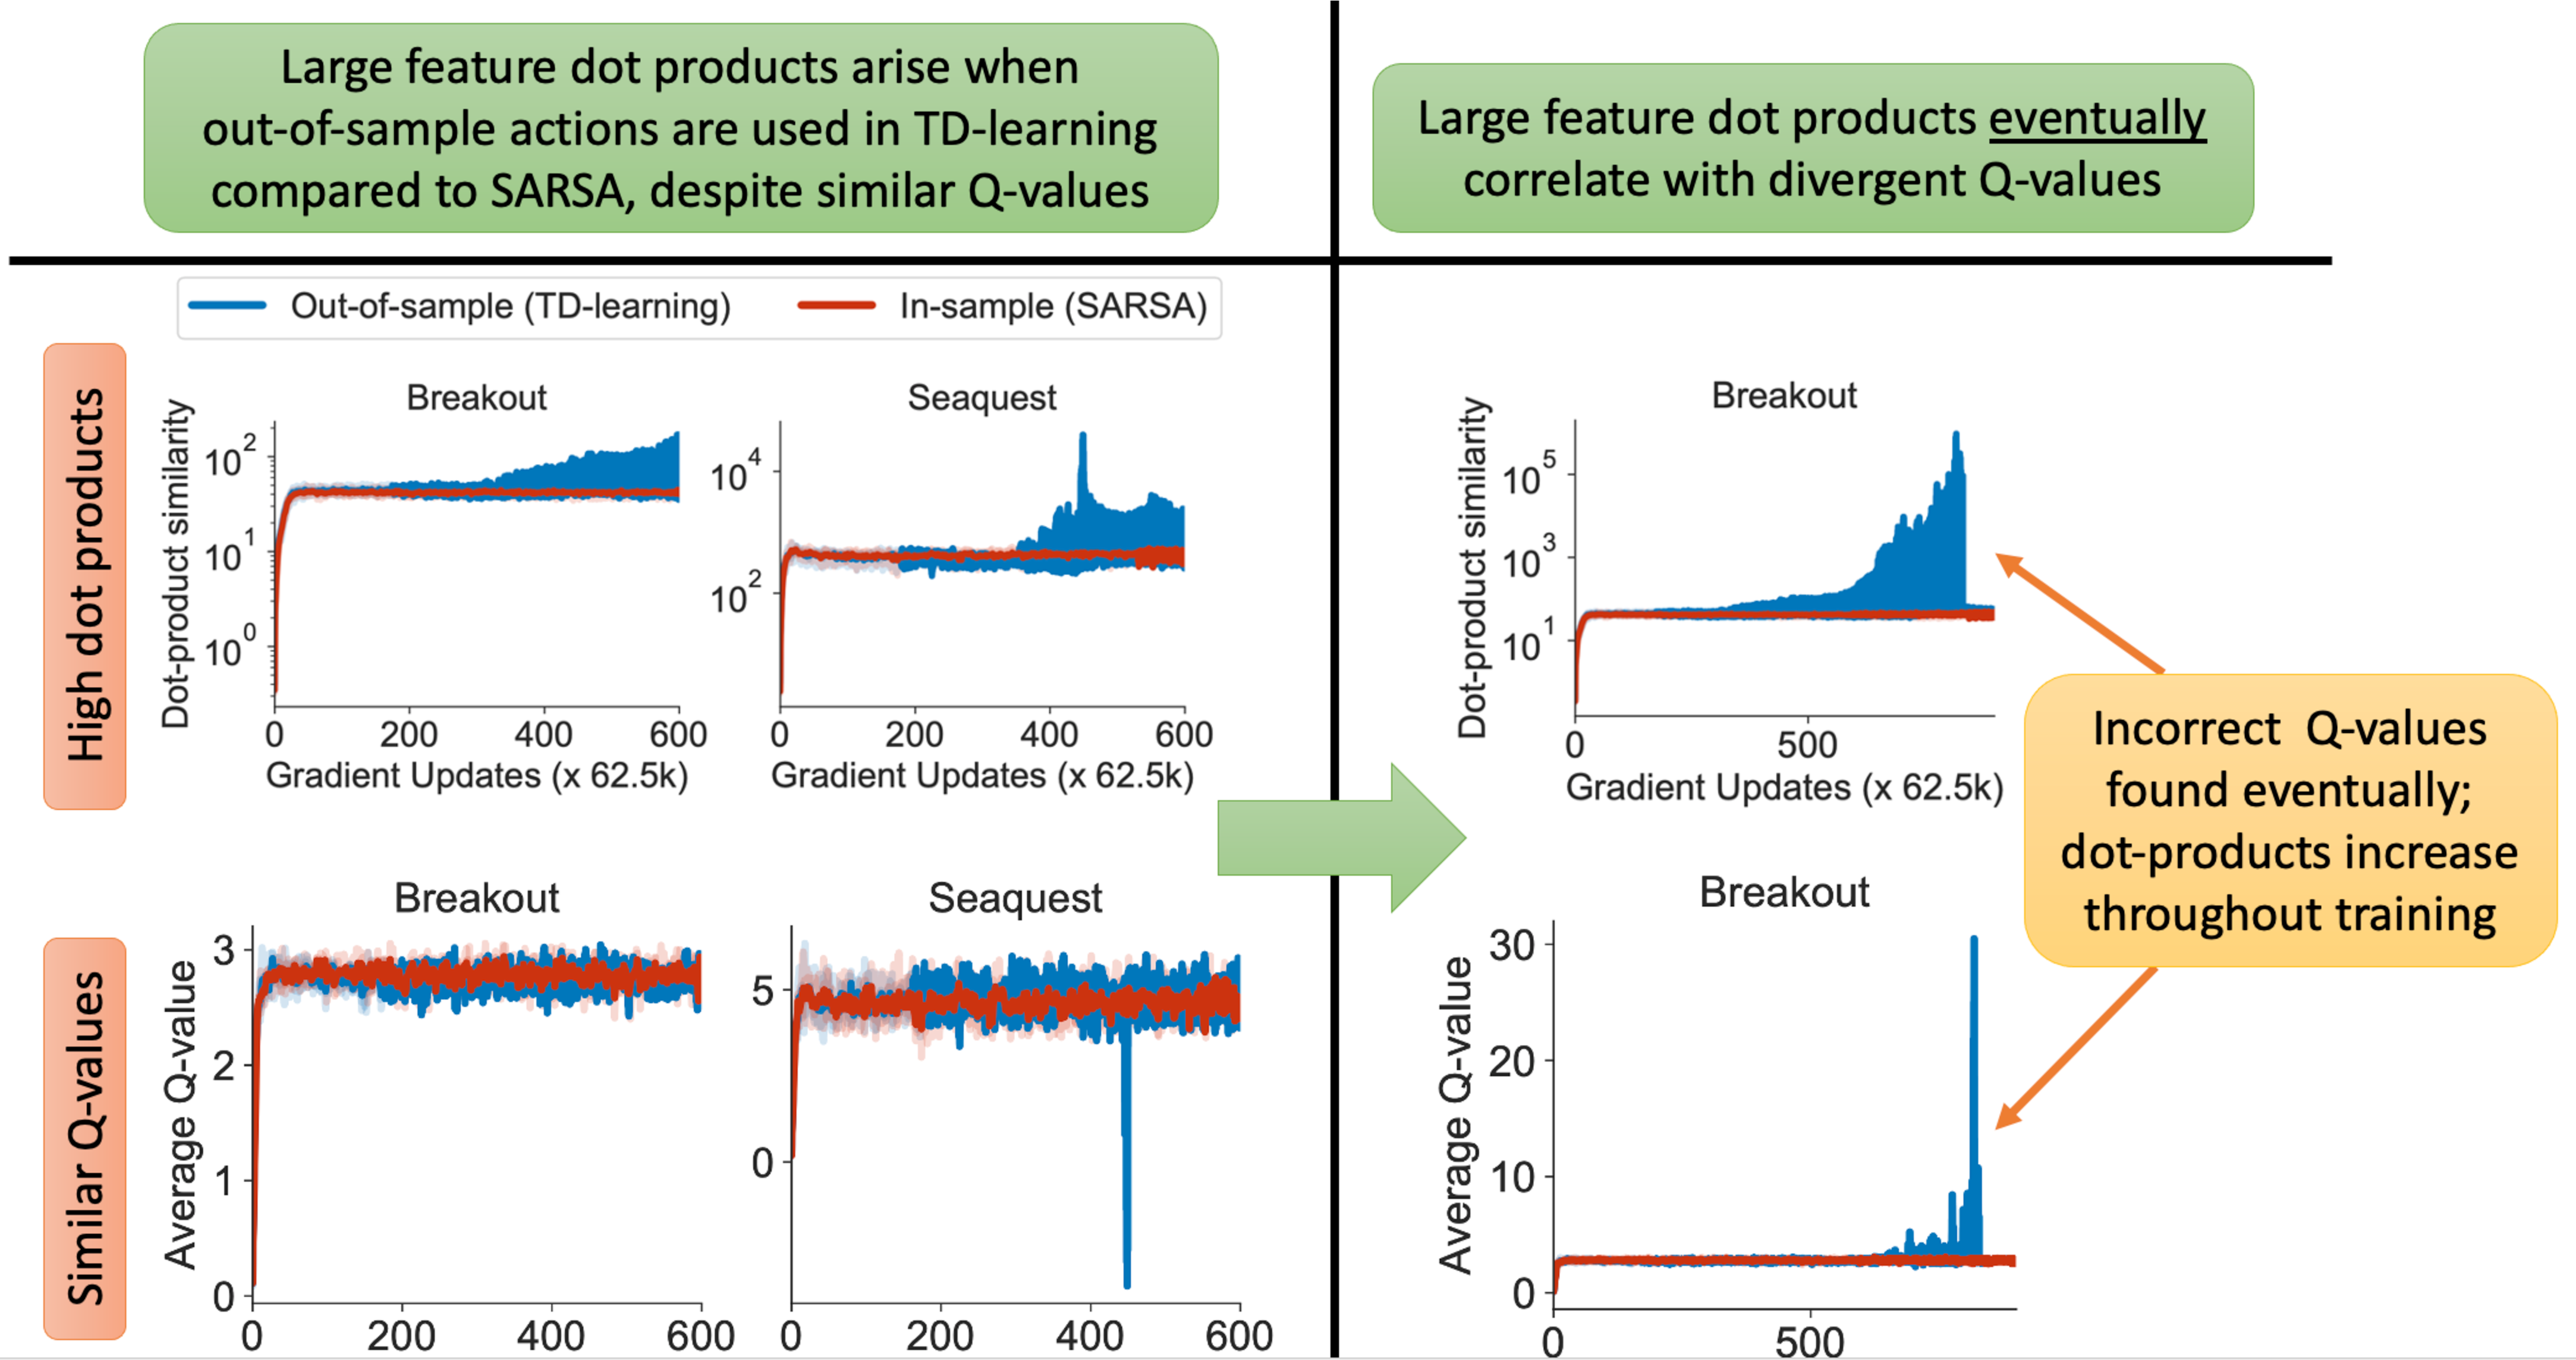
\includegraphics[width=0.67\linewidth]{figures_iclr/final_plot.pdf}~\vline~\vline~
    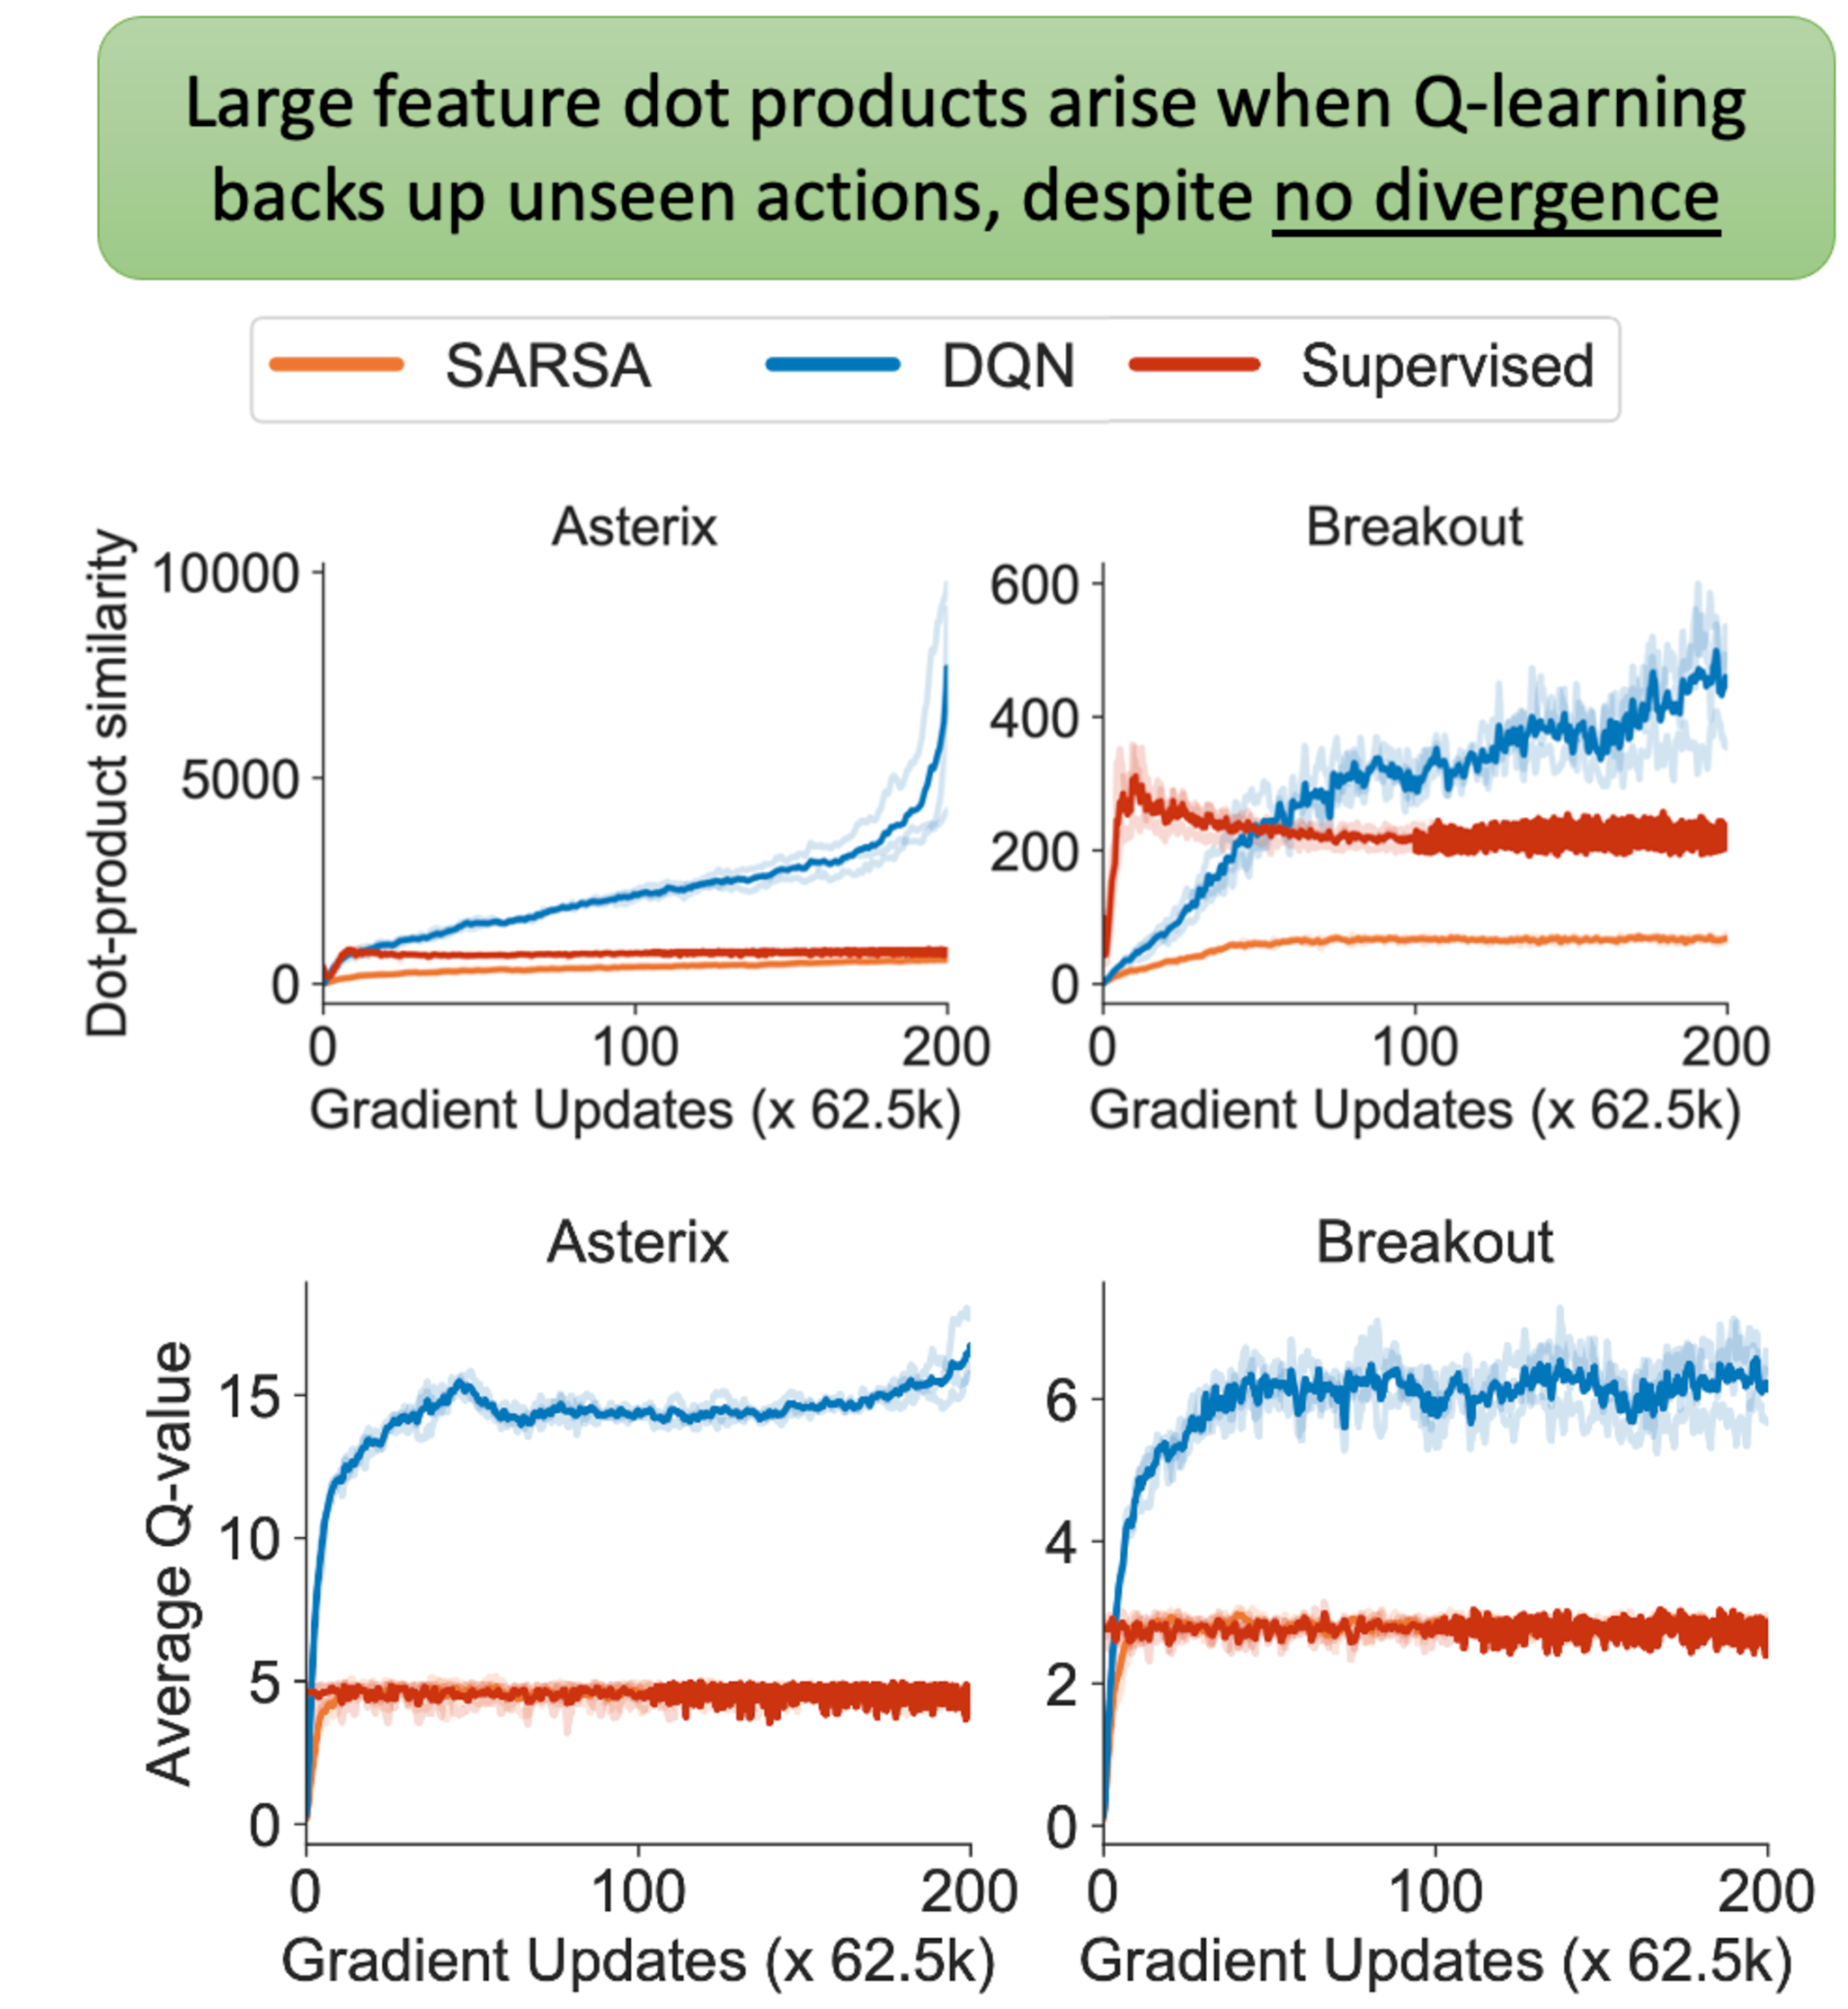
\includegraphics[width=0.32\linewidth]{figures_iclr/final_dqn_fig.pdf}
    \vspace{-0.3cm}
    \caption{\small{Feature dot-products $\phi(\bs, \ba)^\top \phi(\bs', \ba')$ increase during training when backing up from \emph{out-of-sample} but in-distribution actions (\textbf{TD-learning}: left, \textbf{Q-learning}: right), though the average Q-value converges and stays relatively constant. Using only seen state-action pairs for backups (\textbf{offline SARSA}) or not performing Bellman backups (i.e., \textbf{supervised regression}) avoids this issue, with stable and relatively low dot products. \textit{Left}: TD-learning with high feature dot products eventually destabilizes and produces incorrect Q-values, \textit{Right}: DQN attains extremely large feature dot products, despite a relatively stable trend in Q-values.}}  
    \label{fig:dot_products}
    \vspace{-0.6cm}
\end{figure}

\vspace{-5pt}
\subsection{Feature Co-Adaptation And How It Relates To Implicit Regularization}
\label{app:problem_more}
\vspace{-5pt}
In this section, we empirically identify a \emph{feature co-adaptation} phenomenon that appears when training value functions via bootstrapping, where the feature representations of consecutive state-action pairs exhibit a large value of the dot product $\phi(\bs, \ba)^\top \phi(\bs', \ba')$. Note that feature co-adaptation may arise because of high cosine similarity or because of high feature norms. Feature co-adaptation appears even when there is no explicit objective to increase feature similarity.

\textbf{Experimental setup.} We ran supervised regression and three variants of approximate dynamic programming (ADP)
on an offline dataset consisting of 1\% of uniformly-sampled data from the replay buffer of DQN on two Atari games, previously used in \citet{agarwal2019optimistic}. First, for comparison, we trained a Q-function via \textbf{supervised regression} to Monte-Carlo~(MC) return estimates on the offline dataset to estimate the value of the behavior policy. Then, we trained variants of ADP which differ in the selection procedure for the action $\ba'$ that appears in the target value in $\mathcal{L}_\mathrm{TD}(\theta)$ (Equation~\ref{eqn:td_error}). The \textbf{offline SARSA} variant aims to estimate the value of the behavior policy, $Q^{\pi_\beta}$, and sets $\ba'$ to the actual action observed at the next time step in the dataset, such that $(\bs', \ba') \in \mathcal{D}$. The \textbf{TD-learning} variant also aims to estimate the value of the behavior policy, but utilizes the expectation of the target Q-value over actions $\ba'$ sampled from the behavior policy $\pi_\beta$, $\ba' \sim \pi_\beta(\cdot|\bs')$. We do not have access to the functional form of $\pi_\beta$ for the experiment shown in Figure~\ref{fig:dot_products} since the dataset corresponds to the behavior policy induced by the replay buffer of an online DQN, so we train a model for this policy using supervised learning. However, we see similar results comparing \textbf{offline SARSA} and \textbf{TD-learning} on a gridworld domain where we can access the exact functional form of the behavior policy in Appendix~\ref{app:exact_behavior_policy}. %Unlike SARSA, this action $\ba'$ may be different from the one in $\mathcal{D}$, though it comes from the same distribution.
All of the methods so far estimate $Q^{\pi_\beta}$ using different target value estimators.
We also train \textbf{Q-learning}, which chooses the action $\ba'$ to maximize the learned Q-function. While Q-learning learns a different Q-function, we can still compare the relative stability of these methods to gain intuition about the learning dynamics. %To measure feature co-adaptation, we track the average dot product between the learned features at consecutive state-action tuples, $\text{sim}(\bs, \ba, \bs', \ba') := \phi(\bs, \ba)^\top \phi(\bs', \ba')$. 
In addition to feature dot products $\phi(\bs, \ba)^\top \phi(\bs', \ba')$, we also track the average prediction of the Q-network over the dataset to measure whether the predictions diverge or are stable in expectation.

%%AK: also need to figure out an arrangement for figures in the paper
\textbf{Observing feature co-adaptation empirically.} As shown in Figure~\ref{fig:dot_products} (right), the average dot product (top row) between features at consecutive state-action tuples continuously increases for both Q-learning and TD-learning (after enough gradient steps), whereas it flatlines and converges to a small value for supervised regression. We might at first think that this is simply a case of Q-learning failing to converge. However, the bottom row shows that the average Q-values do in fact converge to a stable value. Despite this, the optimizer drives the network towards higher feature dot products. There is no explicit term in the TD error objective that encourages this behavior, 
% and in fact the TD error relatively stays flat \textcolor{red}{(Figure ??)} during training, 
indicating the presence of some implicit regularization phenomenon. This \emph{implicit} preference towards maximizing the dot products of features at consecutive state-action tuples is what we call ``feature co-adaptation.''

\textbf{When does feature co-adaptation emerge?} Observe in Figure~\ref{fig:dot_products} (right) that the feature dot products for offline SARSA converge quickly and are relatively flat, similarly to supervised regression. This indicates that utilizing a bootstrapped update alone is not responsible for the increasing dot-products and instability, because while offline SARSA uses backups, it behaves similarly to supervised MC regression. Unlike offline SARSA, feature co-adaptation emerges for TD-learning, which is surprising as TD-learning also aims to estimate the value of the behavior policy, and hence should match offline SARSA in expectation. The key difference is that while offline SARSA always utilizes actions $\ba'$ observed in the training dataset for the backup, TD-learning may utilize potentially unseen actions $\ba'$ in the backup, even though these actions $\ba' \sim \pi_\beta(\cdot|\bs')$ are \emph{within} the distribution of the data-generating policy. This suggests that utilizing \textbf{out-of-sample} actions in the Bellman backup, even when they are not out-of-distribution, critically alters the learning dynamics. This is distinct from the more common observation in offline RL, which attributes training challenges to out-of-distribution actions~\citep{levine2020offline}, but not out-of-sample actions. The theoretical model developed in Section~\ref{sec:theory} will provide an explanation for this observation with a discussion about how feature co-adaption caused due to out-of-sample actions can be detrimental in offline RL. 

% While action $\ba'$ can be out-of-distribution in the case of Q-learning, this action is sampled from the data-generating distribution of the behavior policy for TD-learning and is hence, not out-of-distribution in this case.

%%AK: does it feel like a jump here, or is it fine?
% The only difference between offline SARSA and Q-learning is whether unseen actions are used to compute the Bellman target\gjt{I don't think that is an accurate statement. The action selection mechanism is different.}:
%%SL.9.17: Yeah, this is correct. Maybe it would be better to mention the TD thing as well in the first paragraph, rather than introducing it for the first time in this paragraph below? That would avoid one very likely criticism you would otherwise get about the comparison between SARSA and Q-learning being non-sensical because they are just learning totally different things
% while $(\bs', \ba')$ used in Q-learning may be unobserved in $\mathcal{D}$, the $(\bs', \ba')$ tuples used in SARSA appear in the dataset, i.e., $(\bs', \ba') \in \mathcal{D}$÷.
%%SL.9.17: some readers won't understand why
% Thus, we might wonder if the use of OOD actions in the backup is the primary culprit for the difference in the observed trends. 

% To understand if this is the case, in Figure~\ref{fig:dot_products} (left), we compare offline SARSA to another variant that we call \textbf{TD-learning},
% %%AK: need to rename TD-learning to something else?
% which utilizes potentially unseen but in-distribution actions sampled from the behavior policy for the Bellman update, such that $\ba' \sim \pi_\beta(\cdot|\bs')$. Like offline SARSA, TD-learning also aims to estimate the value of the behavior policy $Q^{\pi_\beta}$, but it differs from offline SARSA in that the actions $\ba'$ are sampled from the data-generating distribution of the behavior policy. Thus, while they are not \emph{out-of-distribution}, they are also generally not actions that were seen in the dataset $\mathcal{D}$, in contrast to offline SARSA.
% %%SL.9.17: This paragraph is already really hard to read, adding a footnote that creates another branch point for the reader creates an overwhelming cognitive load. Try to merge this footnote into the paragraph, and generally just shorter, more concise, and more digestible sentences.
% % to compute the value of the behavior policy $Q^{\pi_\beta}$. \textbf{Offline SARSA} and \textbf{TD-learning} should match in expectation. 
% As expected, we observe in Figure~\ref{fig:dot_products} (left) that the Q-values predicted by TD-learning match those learned by \textbf{offline SARSA}. However, in contrast to \textbf{offline SARSA}, we find that the dot product similarity for TD-learning increases after enough gradient steps, and this is accompanied by instability in the Q-values. This trend is absent in offline SARSA. This suggests that utilizing out-of-sample actions (even when they are not OOD) in the Bellman backup critically alters the learning dynamics. The theoretical model developed in Section~\ref{sec:theory} provides an explanation for this observation. 
%%AK: one concern: we overload "TD-learning" to mean generic bootstrapping algorithms as well as the "TD learning" baseline we plot. Should we change one of them to something else? Like calling TD-learning generically as bootstrapping and TD learning baseline as FQE.

%%SL.9.17: You can probably shorten this paragraph if you want to save some space
 
% What is the implicit mechanism causing co-adaptation, and why does it occur only when using out-of-sample state-action tuples for the backup? This issue is not corrected by existing offline RL methods, which only avoid out-of-distribution actions~\citep{levine2020offline}, so how does co-adaptation affect offline RL performance? In the next section, we will show how an implicit regularization effect that is studied as a potential benefit of SGD in supervised deep learning can explain this phenomenon, and how this leads to a number of issues in the RL setting.

% \textbf{How do Bellman backups with out-of-sample actions behave?} 
% As shown in Figure~\ref{fig:dot_products} (left), with \textbf{TD-learning}, the dot products steadily increase during training though the average Q-value predictions are roughly constant over the this phase. These Q-values on average match those learned by \textbf{offline SARSA} and \textbf{supervised regression},
% %%SL.7.13: Supervised regression doesn't appear in the left plots!
% but the dot products for \textbf{SARSA} and supervised learning remain flat. In contrast, with \textbf{TD-learning}, the dot products increase after too many gradient steps, and this is accompanied by instability in the Q-values, which then diverge. Note that the only difference between \textbf{TD-learning} and \textbf{SARSA} is the resampling of the target value action, where \textbf{TD-learning} uses a new (out-of-sample) action from the same distribution, while \textbf{SARSA} uses the dataset action.
% %these two approaches quickly converge over the course of training unlike \textbf{TD-learning}. With more training, we find that \textbf{TD-learning} exhibits unstable Q-values, which eventually diverge, whereas the predictions for both \textbf{offline SARSA} and \textbf{supervised regression} converge and do not destabilize with more training.
% % Notably, with \textbf{TD-learning}, the dot-products steadily increase during training and the Q-values eventually diverge, whereas both the dot-products and Q-values of \textbf{offline SARSA} and \textbf{supervised regression} quickly converge and remain stable throughout training (Figure 2). 
% These observations indicate that Bellman backups alone are not responsible for the increasing dot-products and instability because \textbf{offline SARSA} uses Bellman backups, but behaves similarly to \textbf{supervised regression}.
% %%SL.7.13: Again, this is not apparent from the figure, because supervised regression is not shown on the left side!
% On the other hand, \textbf{TD-learning}, which uses out-of-sample actions in the Bellman backup, exhibits increasing dot-products, which eventually ends in  instability, suggesting that out-of-sample actions critically alter the learning dynamics. The theoretical model developed in Section~\ref{sec:theory} provides an explanation for this observation.

% Next, we train two methods that estimate the value of the behavior policy that generated the dataset via dynamic programming. The first approach, which we refer to as  standard \textbf{TD-learning}, estimates $Q^{\pi_\beta}$ by minimizing TD-error $\mathcal{L}_\mathrm{TD}(\theta)$ (Equation in Section~\ref{sec:background}), 
% % $\sum_{\bs, \ba, \bs' \in \mathcal{D}, \ba' \sim {\pi}_\beta(\cdot | \bs')} \left(R(\bs, \ba) + \gamma \bar{Q}_\theta(\bs', \ba') - Q_\theta(\bs, \ba) \right)^2$, 
% where the action $\ba' \sim {\pi}_\beta(\cdot|\bs)$ is sampled from the behavior policy and can be \textit{out-of-sample} for the training dataset, i.e., $(\bs', \ba') \notin \mathcal{D}$, but is \emph{in-distribution}. \aviral{This version is implemented by first learning a model of the behavior policy using supervised classification.} The second approach, which we refer to as \textbf{offline SARSA}, performs Bellman backups from the exact $(\bs', \ba')$ tuple observed in the dataset $\mathcal{D}$ (i.e., $\ba'$ appearing in $\mathcal{L}_\mathrm{TD}(\theta)$ is observed in $\mathcal{D}$).
% % minimizing $\sum_{\bs, \ba, \bs', \ba' \in \mathcal{D}} \left(R(\bs, \ba) + \gamma \bar{Q}_\theta(\bs', \ba') - Q_\theta(\bs, \ba) \right)^2$). 
% Offline SARSA is the same as TD-learning in expectation. However, TD-learning uses potentially out-of-sample actions\footnote{Note that these actions are sampled from the data generating distribution, hence are not out-of-distribution, but may be absent from the training dataset.} in the backup.   As we will show, utilizing out-of-sample state-action tuples in the backup plays a critical role in the learning dynamics.
% Finally, we also train standard \textbf{Q-learning}, which chooses actions $\ba'$ that maximize the learned Q-function. Such actions are also out-of-sample.  


%%SL.7.13: My high-level comment on this section is the following: Right now, your analysis launches into the out-of-sample action discussion right away, without adequately explaining feature co-adaptation. This feels like it's putting the cart before the horse -- before the reader has fully appreciated or even understood what co-adaptation means, they are confronted with this somewhat nuanced discussion about out-of-sample actions. Maybe we should have a couple of sentences before this that basically say "notice how the feature dot products tend to go up right around the same time that things get unstable, isn't that funny? this is what we call feature co-adaptation, let's see what kinds of methods have this issue, and what kinds don't" -- this could be written in just a few sentences, and it should come *before* the discussion of out-of-sample actions, which is secondary to this.


% \begin{figure}[t]
%     \centering
%     \vspace{-5pt}
%     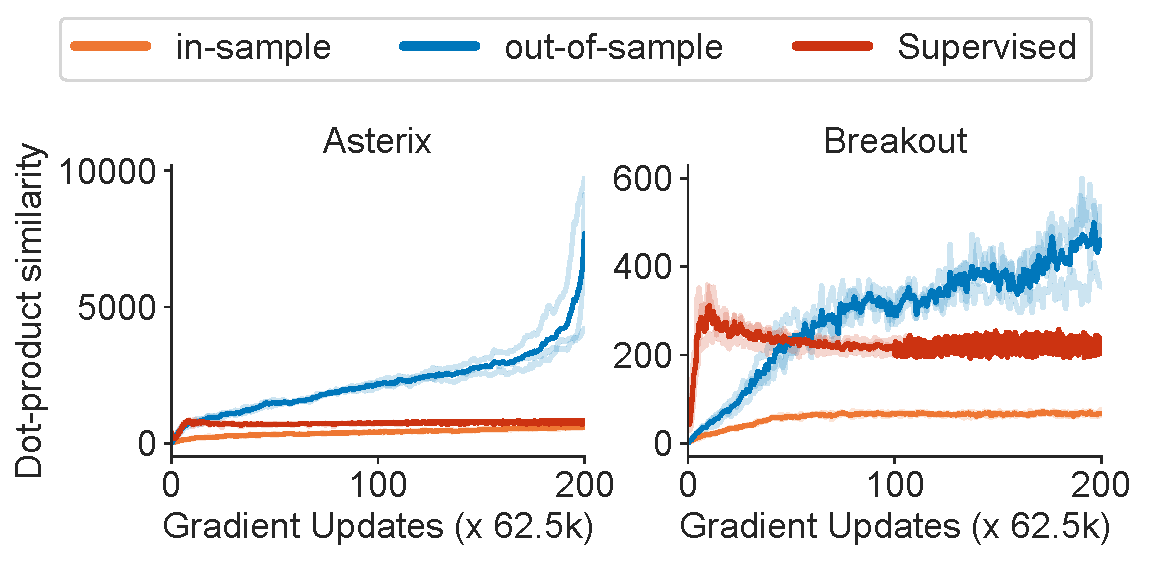
\includegraphics[width=0.45\linewidth]{figures/figure1_dotproduct_dot_products_final.pdf}\\
%     ~~~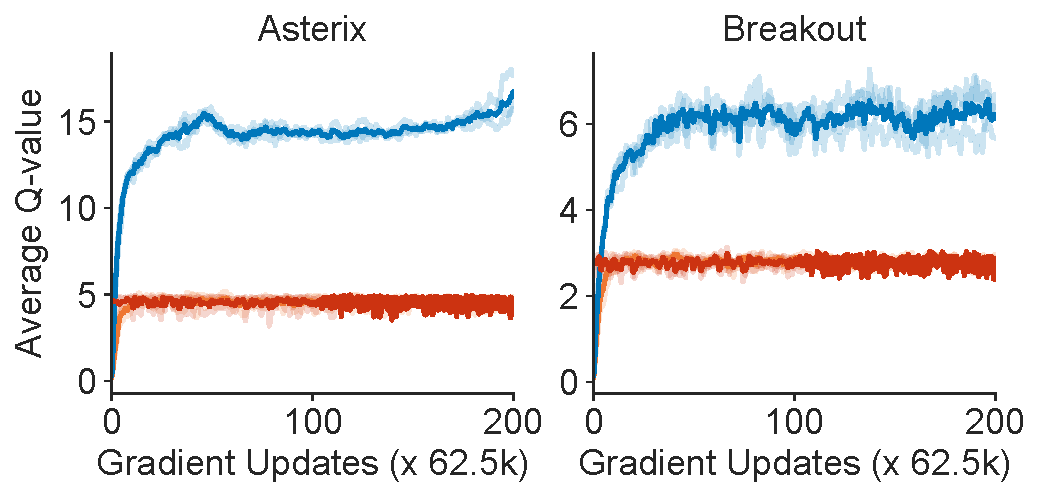
\includegraphics[width=0.45\linewidth]{section3_figs/figure1_dotproduct_q_values (1).pdf}
%     \vspace{-0.24cm}
%     %%SL.5.22: Let's not label it "MC", that's not very informative. Call it "supervised" instead.
%     %%AK: TODO for me, will change it. 
%     %%AK: change labels here
%     \caption{\small{Dot-product $\text{sim}(\bs, \ba, \bs', \ba')$ increases through training when backing up from out-of-sample actions though the average Q-value stays relatively constant, whereas utilizing seen state-action pairs for backups or supervised learning exhibit near-constant dot product similarities as well.}}  
%     \label{fig:dot_products}
%     \vspace{-0.6cm}
% \end{figure}
% \textbf{How do Bellman backups with out-of-sample actions behave?} 
% As shown in Figure~\ref{fig:dot_products} (left), with \textbf{TD-learning}, the dot products steadily increase during training though the average Q-value predictions are roughly constant over the this phase. These Q-values on average match those learned by \textbf{offline SARSA} and \textbf{supervised regression},
% %%SL.7.13: Supervised regression doesn't appear in the left plots!
% but the dot products for \textbf{SARSA} and supervised learning remain flat. In contrast, with \textbf{TD-learning}, the dot products increase after too many gradient steps, and this is accompanied by instability in the Q-values, which then diverge. Note that the only difference between \textbf{TD-learning} and \textbf{SARSA} is the resampling of the target value action, where \textbf{TD-learning} uses a new (out-of-sample) action from the same distribution, while \textbf{SARSA} uses the dataset action.
% %these two approaches quickly converge over the course of training unlike \textbf{TD-learning}. With more training, we find that \textbf{TD-learning} exhibits unstable Q-values, which eventually diverge, whereas the predictions for both \textbf{offline SARSA} and \textbf{supervised regression} converge and do not destabilize with more training.
% % Notably, with \textbf{TD-learning}, the dot-products steadily increase during training and the Q-values eventually diverge, whereas both the dot-products and Q-values of \textbf{offline SARSA} and \textbf{supervised regression} quickly converge and remain stable throughout training (Figure 2). 
% These observations indicate that Bellman backups alone are not responsible for the increasing dot-products and instability because \textbf{offline SARSA} uses Bellman backups, but behaves similarly to \textbf{supervised regression}.
% %%SL.7.13: Again, this is not apparent from the figure, because supervised regression is not shown on the left side!
% On the other hand, \textbf{TD-learning}, which uses out-of-sample actions in the Bellman backup, exhibits increasing dot-products, which eventually ends in  instability, suggesting that out-of-sample actions critically alter the learning dynamics. The theoretical model developed in Section~\ref{sec:theory} provides an explanation for this observation.

%To discern the differences between TD-learning and supervised learning, we first note in Figure~\ref{fig:dot_products} (right) that both the Q-value predictions and dot-product values quickly stabilize for \textbf{supervised regression} (shown in red). A similar convergent behavior in both dot products and learned Q-values is observed when utilizing in-sample actions in the case of \textbf{offline SARSA}, even though SARSA uses Bellman backups (Figure~\ref{fig:dot_products}, ``in-sample''). Next, we turn to case of \textbf{TD-learning}, which utilizes out-of-sample actions. We would expect TD-learning to converge to the same solution as offline SARSA, and we indeed observe similar Q-values in average (compare red vs blue lines in Figure~\ref{fig:dot_products} (left)), however, crucially the feature dot product values are much larger for TD-learning. In fact, the feature dot products in TD-learning continually increase with more training (Figure~\ref{fig:dot_products}) while it stabilizes for offline SARSA. This indicates that even though the Q-function outputs similar values, performing Bellman backups with out-of-sample actions gives rise to increasing dot-product values. Furthermore, as shown in Figure~\ref{fig:dot_products} (middle), once the values of dot-products are large enough (after more training steps), training further leads to an unstable trend in Q-values.


% \vspace{-5pt}

\vspace{-0.2cm}
\subsection{Theoretically Characterizing Implicit Regularization in TD-Learning}
\label{sec:dr3_theory} 
\vspace{-0.2cm}
Why does feature co-adaptation emerge in TD-learning and what do \emph{out-of-sample} actions have to do with it? To answer this question, we theoretically characterize the implicit regularization effects in TD-learning. We analyze the learning dynamics of TD learning in the overparameterized regime, where there are many different parameter vectors $\theta$ that fully minimize the training set temporal difference error. We base our analysis of TD learning on the analysis of implicit regularization in supervised learning, previously developed by \citet{blanc2020implicit,damian2021label}.

\textbf{Background.} When training an overparameterized $f_\theta(\bx)$ via supervised regression using the squared loss, denoted by $L$, many different values of $\theta$ will satisfy $L(\theta)=0$ on the training set due to overparameterization, but \citet{blanc2020implicit} show that the dynamics of stochastic gradient descent will only find fixed points $\theta^*$ that additionally satisfy a condition which can be expressed as $\nabla_\theta R(\theta^*) = 0$, along certain directions (that we will describe shortly). This function $R(\theta)$ is referred to as the implicit regularizer. The noisy gradient updates analyzed in this model have the form:  
\vspace{-0.05in}
\begin{align}
\label{eq:gradient_update}
    \theta_{k+1} \leftarrow \theta_k - \eta \nabla_\theta L(\theta) + \eta \varepsilon_k, ~~ \varepsilon_k \sim \mathcal{N}(0, M).
\end{align}
\citet{blanc2020implicit} and \citet{damian2021label} show that some common SGD techniques fall into this framework, for example, when the regression targets in supervised learning are corrupted with $\mathcal{N}(0, 1)$ label noise, then the resulting $M = \sum_{i=1}^{|\mathcal{D}|} \nabla_\theta f_\theta(\bx_i) \nabla_\theta f_\theta(\bx_i)^\top$ and the induced implicit regularizer $R$ is given by $R(\theta) = \sum_{i}^{|\mathcal{D}|} ||\nabla_\theta f_\theta(\bx_i)||_2^2$. Any solution $\theta^*$ found by Equation~\ref{eq:gradient_update} must satisfy $\nabla_\theta R(\theta^*) = 0$ along directions $\bv \in \mathbb{R}^{|\theta|}$ which lie in the null space of the Hessian of the loss $\nabla^2_\theta L(\theta^*)$ at $\theta^*$,  $\bv \in \text{Null}(\nabla^2_\theta L(\theta^*))$. The intuition behind the implicit regularization effect is that along such directions in the parameter space, the Hessian is unable to contract $\theta_k$ when running noisy gradient updates (Equation~\ref{eq:gradient_update}). Therefore, the only condition that the noisy gradient updates converge/stabilize at $\theta^*$ is given by the condition that $\nabla R(\theta^*) = 0$. This model corroborates findings~\citep{mulayoff2020unique, damian2021label} about the solutions from SGD, which motivates our use. 

\textbf{Our setup.} Following this framework, we analyze the fixed points of noisy TD-learning. We consider noisy pseudo-gradient (or semi-gradient) TD updates with a general noise covariance $M$:
\vspace{-0.05in}
\begin{align}
    \theta_{k+1} = \theta_k - \eta \underbrace{\left( \sum_i \nabla_\theta Q(\bs_i, \mathbf{a}_i) \left(Q_\theta(\bs_i, \mathbf{a}_i)\!- \!(r_i\!+\!\gamma {Q}_{\theta}(\bs'_i, \mathbf{a}'_i))\right) \right)}_{:= g(\theta)} +\eta \varepsilon_k,  ~~ \varepsilon_k \sim \mathcal{N}(0, M)
\label{eq:td_update}
\end{align}
We use a deterministic policy $\mathbf{a}'_i = \pi(\bs'_i)$ to simplify exposition. Following \citet{damian2021label}, we can set the noise model $M$ as $M = \sum_i \nabla_\theta Q(\bs_i, \mathbf{a}_i) \nabla_\theta Q(\bs_i, \mathbf{a}_i)^\top$, or utilize a different choice of $M$, but we will derive the general form first.  Let $\theta^*$ denote a stationary point of the training TD error, such that the pseudo-gradient
$g(\theta^*) = 0$. Further, we denote the derivative of $g(\theta)$ w.r.t. $\theta$ as the matrix $G(\theta) \in \mathbb{R}^{|\theta| \times |\theta|}$, and refer to it as the \emph{pseudo-Hessian}: although $G(\theta)$ is not actually the second derivative of any well-defined objective, since TD updates are not proper gradient updates, as we will see it will play a similar role to the Hessian in gradient descent. For brevity, define $G = G(\theta^*)$, $g = g(\theta^*)$, $\nabla G = \nabla_\theta G(\theta^*) \in \mathbb{R}^{|\theta| \times |\theta| \times |\theta|}$, and let $\lambda_i(P)$ denote the $i$-th eigenvalue of matrix $P$, when arranged in decreasing order of its (complex) magnitude $|\lambda_i(P)|$ (note that eigenvalues can be complex for non-symmetric matrices that we encounter here). 

\textbf{Assumptions.} To simplify analysis, we assume that matrices $G$ and $M$ (i.e., the noise covariance matrix) span the same $n$-dimensional basis in $d$-dimensional space, where $d$ is the number of parameters and $n$ is the number of datapoints, and $n \ll d$ due to overparameterization. We also require $\theta^*$ to satisfy a technical criterion that requires approximate alignment between the eigenspaces of $G$ and the gradient of the Q-function, without which noisy TD may not be stable at $\theta^*$. We summarize all the assumptions in Appendix~\ref{app:dr3_proofs}, and present the resulting regularizer below. 

\begin{tcolorbox}[colback=blue!6!white,colframe=black,boxsep=0pt,top=-3pt,bottom=2pt]
\vspace{2mm}
\begin{theorem}[Implicit regularizer at TD fixed points]
\label{thm:implicit_noise_reg}
Under the assumptions so far, a fixed point of TD-learning,  $\theta^*$, where $Q_{\theta^*}(\bs_i, \mathbf{a}_i) = r_i + \gamma Q_{\theta^*}(\bs'_i, \mathbf{a}'_i)$ for every $(\bs_i, \mathbf{a}_i, \bs'_i) \in \mathcal{D}$ is stable (atttractive) if: \textbf{(1)} it satisfies $\mathrm{Re}(\lambda_i(G)) \geq 0, \forall i$ and $\mathrm{Re}(\lambda_i(G)) > 0$ if $|\mathrm{Imag}(\lambda_i(G))| > 0$, and \textbf{(2)} along directions $\bv \in \mathbb{R}^{\text{dim}(\theta)}, \bv \in \text{Null}(G)$, $\theta^*$ is the stationary point of the implicit regularizer:
\vspace{-0.2cm}
\begin{align}
\label{eqn:regularizer}
\!\!\!\!R_\mathrm{TD}(\theta)\!\!&=\!\!\underbrace{\eta \sum_{i=1}^{|\mathcal{D}|} \nabla Q_\theta(\bs_i, \mathbf{a}_i)^\top \Sigma^{*}_M \nabla Q_\theta(\bs_i, \mathbf{a}_i)}_{\text{implicit regularizer for noisy GD}}
\!\!\!-\!\!\!\underbrace{\eta \gamma \sum_{i=1}^{|\mathcal{D}|} \mathrm{tr}\left(\left[\left[\nabla Q_\theta(\bs'_i, \mathbf{a}'_i)^\top\right]\right]^\top \Sigma_M^* \nabla Q_\theta(\bs_i, \mathbf{a}_i)  \right)}_{\text{additional term in TD learning}}
%%SL.10.27: would it be better to write the trace term as gradQ^T sigma gradQ (since tr(sigma gradQ gradQ^T) = tr(gradQ^T sigma gradQ))? that might make the similarity (but subtle difference) between the two terms more apparent...
    % R_\mathrm{TD}(\theta) = \sum_{i=1}^{|\mathcal{D}|} \mathrm{trace}\left[ \Sigma^{* \top}_M \nabla_\theta Q_\theta(\bs_i, \mathbf{a}_i) \left( \nabla_\theta Q_\theta(\bs_i, \mathbf{a}_i) - \gamma \texttt{Stop}(\nabla_\theta Q_\theta(\bs'_i, \mathbf{a}'_i)) \right)^\top \right].  
    %%SL.9.29: I think it might be clearer if you write this as a difference of two terms, because then the first term will look like the supervised R(theta), but the second one will look clearly weird. The first term then becomes gradQ^T Sigma^T gradQ (and you don't need trace), which is very intuitive (also, Sigma is symmetric, right? so is the transpose symbol there necessary?). Additionally, consider using a less jarring symbol for Stop, so that the equation is typeset so that it looks more like -grad Q [gradQ^T] or something and the stop part is unobtrusive -- that would make it easier for readers to get intuition for what this equation means. Currently it's extremely hard to understand from looking at it.
\end{align}
% \vspace{-0.1in}
where $(\bs_i, \mathbf{a}_i)$ and $(\bs'_i, \mathbf{a}'_i)$ denote state-action pairs that appear together in a Bellman update, $[[\square]]$ denotes the stop-gradient function, which does not pass partial gradients w.r.t. $\theta$ into $\square$. $\Sigma^*_M$ is the fixed point of the  discrete Lyapunov equation: $$\Sigma^*_M := (I - \eta G) \Sigma^*_M (I - \eta G)^\top + \eta^2 M.$$
\end{theorem}
\vspace{1mm}
\end{tcolorbox}
A proof of Theorem~\ref{thm:implicit_noise_reg} is provided in Appendix~\ref{app:dr3_proofs}. Next, we explain the intuition behind this result and provide a proof sketch. To derive the induced implicit regularizer for a stable fixed point $\theta^*$ of TD error, we study the learning dynamics of noisy TD learning (Equation~\ref{eq:td_update}) initialized at $\theta^*$, and derive conditions under which this noisy update would stay close to $\theta^*$ with multiple updates.  This gives rise to the two conditions shown in Theorem~\ref{thm:implicit_noise_reg} which can be understood as controlling stability in mutually exclusive directions in the parameter space. If condition \textbf{(1)} is not satisfied, then even under-parameterized TD will diverge away from $\theta^*$, since $I - \eta G$ would be a non-contraction as the spectral radius, $\rho(I - \eta G) \geq 1$ in that case. Thus, $\theta_k - \theta^*$ will grow or not decrease in some direction. When \textbf{(1)} is satisfied for all directions in the parameter space, there are still directions where both the real and imaginary parts of the eigenvalue $\lambda_i(G)$ are $0$ due to overparameterization\footnote{To see why this is the case, note that $\text{rank}(G) \leq |\mathcal{D}| \ll \text{dim}(\theta)$, and so some eigenvalues of $G$ are $0$.}. 
In such directions, learning is governed by the projection of the noise under the tensor  $\nabla G$,
%%SL.12.5: Are we making that mistake here again where we call the TD pseudo-gradient a derivative? I would recommend being *very* careful about the term derivative. Basically, don't call something a derivative if it's not really a derivative. You can introduce some term for it like pseudo-gradient, but it's very important to clearly distinguish between things that are actual derivatives or gradients, and the TD update. Try to avoid mixing the terminology, but it's OK to define some shorthand term like pseudo-gradient
%%AK: changed it here
which appears in the Taylor expansion of $\theta_k - \theta^*$ around the point $\theta^*$:
\begin{align}
    \label{eqn:nu_k}
    &\theta_{k+1} = \theta_k - \eta \left(g + G (\theta_k - \theta^*) + \frac{1}{2} \nabla G [\theta_k -\theta^*, \theta_k - \theta^*] \right) + \varepsilon_k, ~~ \varepsilon_k \sim \mathcal{N}(0, M)\\
    \implies &\nu_{k+1} = (I - \eta G )\nu_k  - \frac{\eta}{2} \nabla G [\nu_k, \nu_k] + \varepsilon_k,
    \label{eqn:nu_k_actual}
\end{align}
where we reparameterize in terms of $\nu_k := \theta_k - \theta^*$. The proof shows that $\theta^*$ is stable if it is a stationary point of the implicit regularizer $R_\mathrm{TD}$ (condition \textbf{(2)}), which ensures that total noise (i.e., accumulated $\varepsilon_k$ over iterations $k$) accumulated by $\nabla G$ does not lead to a large deviation in $\nu_k$ in directions where $I - \eta G$ does not contract. 
% The total noise accumulated with such noisy backups (Equation~\ref{eqn:nu_k}) admits the covariance matrix $\Sigma^*_M$, and the derivative of the regularizer $\nabla_\theta R_\mathrm{TD}(\theta)$ at an attractive $\theta^*$ must be zero to prevent any deviation in $\nu_k$ in directions where learning is controlled by \textbf{(2)}.   

% To derive the induced implicit regularizer for a stable fixed point $\theta^*$ of TD error, we study the learning dynamics of noisy TD learning (Equation~\ref{eq:td_update}) initialized at $\theta^*$, and derive conditions under which this noisy update would stay close to $\theta^*$ with multiple updates. In this case, we can utilize Taylor expansion around $\theta^*$ to track the evolution of the difference between $\theta_k$ and $\theta^*$, denoted as $\nu_k = \theta_k - \theta^*$ (roughly; modulo some terms we will discuss in Appendix~\ref{app:proofs}), as shown in Equation~\ref{eqn:nu_k}:
% \begin{align}
%     \label{eqn:nu_k}
%     &\theta_{k+1} = \theta_k - \eta \left(g + G (\theta_k - \theta^*) + \frac{1}{2} \nabla G [\theta_k -\theta^*, \theta_k - \theta^*] \right) + \varepsilon_k, ~~ \varepsilon_k \sim \mathcal{N}(0, M)\\
%     \implies &\nu_{k+1} = (I - \eta G )\nu_k  - \frac{\eta}{2} \nabla G [\nu_k, \nu_k] + \varepsilon_k.
%     \label{eqn:nu_k_actual}
% \end{align}
% Our theoretical result derives the implicit regularizer by characterizing conditions on $\theta^*$ that are necessary for the stability of the learning dynamics in Equation~\ref{eqn:nu_k_actual} in the neighborhood around $\theta^*$. 

\textbf{Interpretation of Theorem~\ref{thm:implicit_noise_reg}.} While the choice of the noise model $M$ will change the form of the implicit regularizer, in practice, the form of $M$ is not known as this corresponds to the noise induced via SGD. We can consider choices of $M$ for interpretation, but Theorem~\ref{thm:implicit_noise_reg} is easy to qualitatively interpret for $M$ such that $\Sigma^*_M = I$. In this case, we find that the implicit preference towards local minima of $R_\mathrm{TD}(\theta)$ can explain feature co-adaptation. In this case, the regularizer is simpler:
\begin{align*}
    R_\mathrm{TD}(\theta) := \sum_i ||\nabla Q_\theta(\bs_i, \mathbf{a}_i) ||_2^2 - \gamma \nabla Q_\theta(\bs_i, \mathbf{a}_i)^\top \nabla [[Q_\theta(\bs'_i, \mathbf{a}'_i)]].
\end{align*}
The first term is equal to the squared per-datapoint gradient norm, which is same as the implicit regularizer in supervised learning obtained by \citet{blanc2020implicit,damian2021label} with label noise. However, $R_\mathrm{TD}(\theta)$ additionally includes a second term that is equal to the dot product of the gradient of the Q-function at the current and next states, $\nabla_\theta Q_\theta(\bs_i, \mathbf{a}_i)^\top \nabla_\theta Q_\theta(\bs'_i, \mathbf{a}'_i)$, and thus this term is effectively \emph{maximized}. When restricted to the last-layer parameters of a neural network,
this term is equal to the dot product of the features at consecutive state-action tuples: $\sum_i \nabla_\theta Q_\theta(\bs_i, \mathbf{a}_i)^\top \nabla_\theta Q_\theta (\bs'_i, \mathbf{a}'_i) = \sum_i \phi(\bs_i, \mathbf{a}_i)^\top \phi(\bs'_i, \mathbf{a}'_i)$. The tendency to maximize this quantity to attain a local minimizer of the implicit regularizer corroborates the empirical findings of increased dot product in Section~\ref{app:problem_more}. 

\textbf{Explaining the difference between utilizing seen and unseen actions in the backup.} If all state-action pairs $(\bs'_i, \mathbf{a}'_i)$ appearing on the right-hand-side of the Bellman update also appear in the dataset $\mathcal{D}$, as in the case of offline SARSA (Figure~\ref{fig:dot_products}), the preference to increase dot products will be balanced by the affinity to reduce gradient norm (first term of $R_\mathrm{TD}(\theta)$ when $\Sigma^*_M = I$): for example, for offline SARSA, when $(\bs'_i, \mathbf{a}'_i)$ are permutations of $(\bs_i, \mathbf{a}_i)$, $R_\mathrm{TD}$ is lower bounded by $(1 - \gamma) \sum_i ||\nabla_\theta Q_\theta(\bx_i)||_2^2$ and hence minimizing $R_\mathrm{TD}(\theta)$ would minimize the feature norm instead of maximizing dot products. This also corresponds to the implicit regularizer we would obtain when training Q-functions via supervised learning and hence, our analysis predicts that offline SARSA with in-sample actions (i.e., when $(\bs', \mathbf{a}') \in \mathcal{D}$) would behave similarly to supervised regression. 

However, the regularizer behaves very differently when unseen state-action pairs $(\bs'_i, \mathbf{a}'_i)$ appear only on the right-hand-side of the backup. This happens with any algorithm where $\mathbf{a}'$ is not the dataset action, which is the case for all deep RL algorithms that compute target values by selecting $\mathbf{a}'$ according to the current policy. In this case, we expect the dot product of gradients at $(\bs, \mathbf{a})$ and $(\bs', \mathbf{a}')$ to be large at any attractive fixed point, since this minimizes $R_\mathrm{TD}(\theta)$. This is precisely a form of co-adaptation: \textit{gradients at out-of-sample state-action tuples are highly similar to gradients at observed state-action pairs measured by the dot product}. This observation is also supported by the analysis in Section~\ref{app:problem_more}. Finally, note that the choice of $M$ is a modelling assumption, and to derive our explicit regularizer, later in the paper, we will make a simplifying choice of $M$. However, we also empirically verify that a different choice of $M$, given by label noise, works well.
%%%%%%%%%%%%%%%%%%%%%%%%%%%%%%%%%%%%%%%%%%%%%%%%%%%%%%%%%%


\begin{figure}[t]
    \centering
    % \vspace{-18pt}
    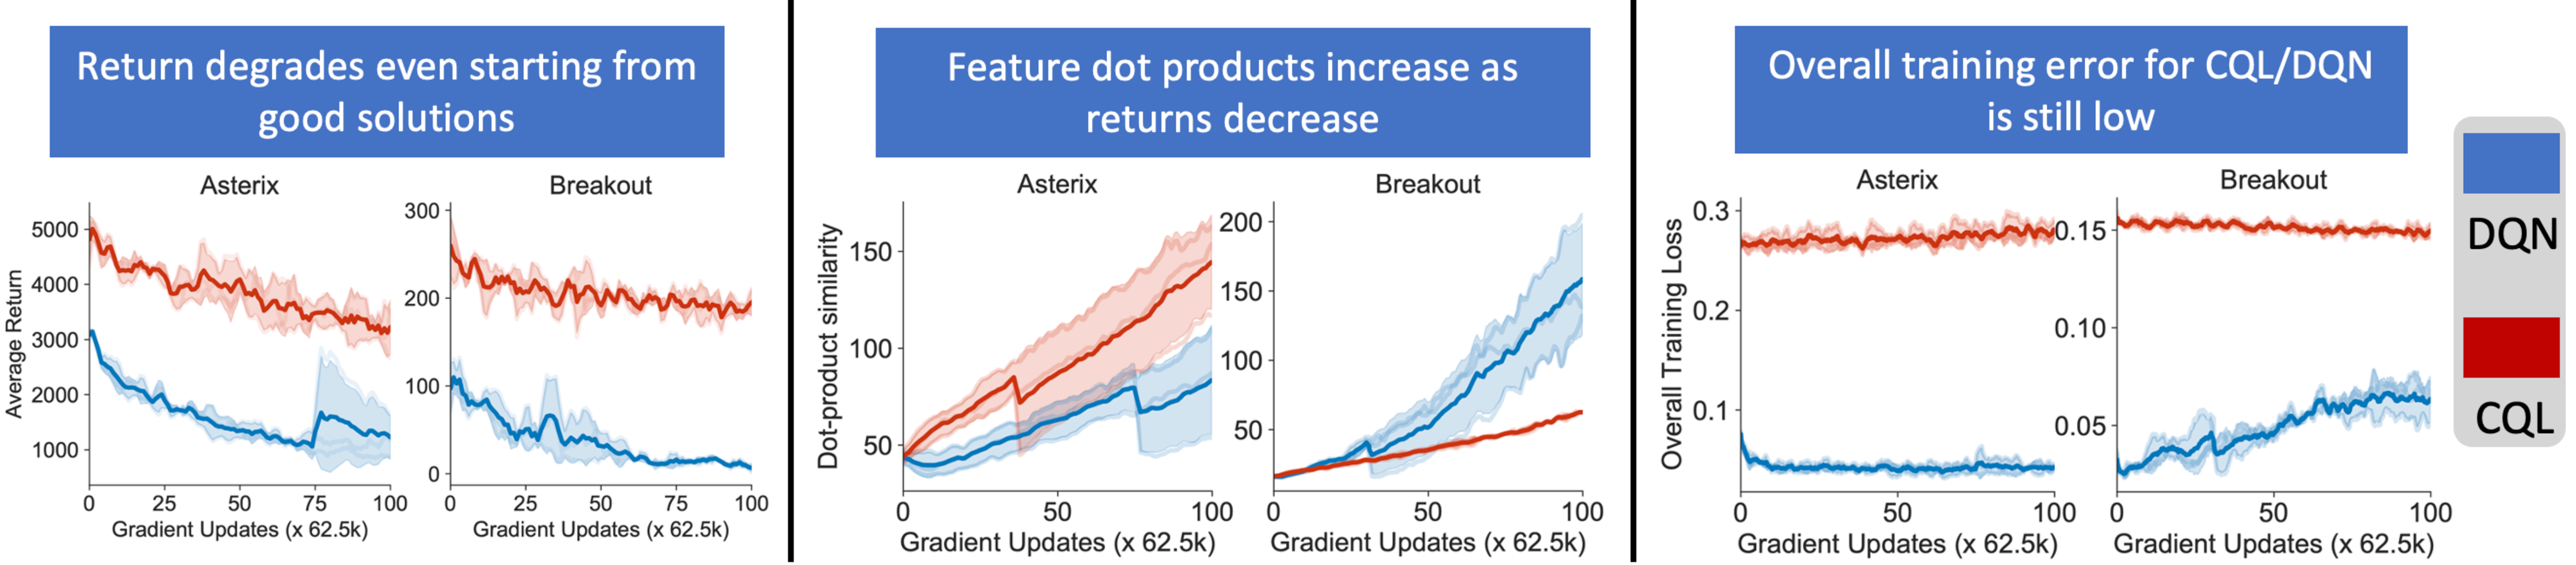
\includegraphics[width=0.99\linewidth]{chapters/dr3/figures_iclr/return_degrades.pdf}
    % 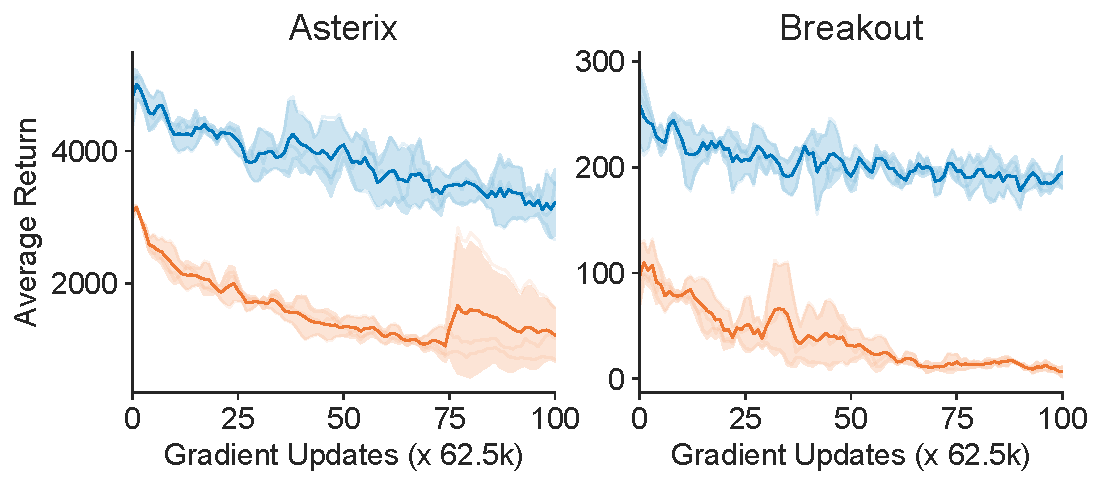
\includegraphics[width=0.49\linewidth]{figures/figure3_neurips_stability_cql_dot_product_both_return.pdf}
    \vspace{-0.3cm}
    \caption{\small{Even when current offline RL algorithms are initialized at a high-performing checkpoint that attains small feature dot products, feature dot products increase with further training and the performance degrades.}}  
    %%SL.7.13: I don't really understand the implication of the last part ("note that the values of the TD error and the overall training loss for either algorithm are generally low and decrease in many cases")
    \label{fig:stability}
    \vspace{-0.3cm}
\end{figure}



\textbf{Why is implicit regularization detrimental to policy performance?}
To answer this question, we present theoretical and empirical evidence that illustrates the adverse effects of this implicit regularizer. Empirically, we ran two algorithms, DQN and CQL, initialized from a high-performing Q-function checkpoint,
%%SL.10.27: This part is going to really throw off some readers. Of course it's not a stable point for TD, because you didn't learn it with TD! Why do we expect the solution found by one method (in this case DR3) to be stable for another method? That doesn't illustrate that TD is bad, just that DR3 changes the fixed point (which it should). But perhaps if you don't want to go into detail about this issue, you could somehow sweep the "obtained using DR3" bit under the rug to avoid distracting the reader?
%%AK: agreed, removed
which attains relatively small feature dot products (i.e., the second term of $R_\mathrm{TD}(\theta)$ is small). Our goal is to see if TD updates starting from such a ``good'' initialization still stay around it or diverge to poorer solutions. Our theoretical analysis in Section~\ref{sec:dr3_theory} would predict that TD learning would destabilize from such a solution, since it would not be a stable fixed point. Indeed, as shown in Figure~\ref{fig:stability}, the policy immediately degrades, and the the dot-product similarities start to increase. This even happens with CQL, which explicitly corrects for distributional shift confounds, implying that the performance drop cannot be directly explained by the typical out-of-distribution action explanations. To investigate the reasons behind this drop, we also measured the training loss function values for these algorithms (i.e., TD error for DQN and TD error + CQL regularizer for CQL) and find in Figure~\ref{fig:stability} that the loss values are generally small for both CQL and DQN. This indicates that the preference to increase dot products is not explained by an inability to minimize TD error. 
%%SL.12.5: I don't understand what "implicit phenomenon" means or how the loss being low indicates this
In Appendix~\ref{app:cql_stability}, we show that this drop in performance when starting from good solutions can be effectively mitigated with our proposed \methodname\ explicit regularizer for both DQN and CQL. Thus we find that not only standard TD learning degrades from a good solution in favor of increasing feature dot products, but keeping small dot products enables these algorithms to remain stable near the good solution.
%%SL.12.5: I slightly tweaked the above sentence, but it can be badly misunderstood as saying that basically our entire evaluation of DR3 has been offloaded into that appendix.

To motivate why co-adapted features can lead to poor performance in TD-learning, we study the convergence of linear TD-learning on co-adapted features. Our theoretical result characterizes a lower bound on the feature dot products in terms of the feature norms for state-action pairs in the dataset $\mathcal{D}$, which if satisfied, will inhibit  convergence: 
\begin{tcolorbox}[colback=blue!6!white,colframe=black,boxsep=0pt,top=-3pt,bottom=2pt]
\vspace{2mm}
\begin{proposition}[TD-learning on co-adapted features]
\label{thm:co_adapted_features_are_bad}
Assume that the features $\Phi = [\phi(\bs, \mathbf{a})]_{\bs, \mathbf{a}}$ are used for linear TD-learning. Then, if 
$$\sum_{\bs, \mathbf{a}, \bs' \in \mathcal{D}} \phi(\bs, \mathbf{a})^\top \phi(\bs', \mathbf{a}') \geq \frac{1}{\gamma} \sum_{\bs, \mathbf{a} \in \mathcal{D}} \phi(\bs, \mathbf{a})^\top \phi(\bs, \mathbf{a}),$$ 
linear TD-learning using features $\Phi$ will not converge. 
\end{proposition}
\end{tcolorbox}
A proof of Proposition~\ref{thm:co_adapted_features_are_bad} is provided in Appendix~\ref{app:new_thm} and it relies on a stability analysis of linear TD. While features change during training for TD-learning with neural networks, and arguably linear TD is a simple model to study consequences of co-adapted features, even in this simple linear setting, Proposition~\ref{thm:co_adapted_features_are_bad} indicates that TD-learning may be non-convergent as a result of co-adaptation.

% \textbf{Comparison to implicit regularization in TD learning with linear function approximation.} Running stochastic gradient descent in overparameterized linear regression finds solutions with the smallest $\ell_2$ norm, which is often regarded as the implicit regularizer. Based on this observation, one might wonder how our derived implicit regularizer relates to minimum norm solutions attained by gradient descent in overparameterized linear TD learning. The implicit regularizer we obtain in  Equation~\ref{eqn:regularizer} would be a constant, independent of the parameter vector $\theta$ for linear TD learning. Thus our regularization specifically captures the effect of SGD on non-linear function approximators, which are absent when studying linear function approximation. 

% \textbf{Takeaways.} We summarize the key takeaways from our theoretical analysis now. \textbf{(1)} \emph{The implicit regularizer at TD fixed points} is shown in Equation~\ref{eqn:regularizer}. The first term corresponds to the regularizer for SGD in supervised learning, while the second term that is unique to TD and leads to an (undesirable) increase in gradient or feature dot products; \textbf{(2)}\emph{Out-of-sample actions exacerbate the implicit regularization effect,} since feature dot products can be easily increased when out-of-sample actions, which do not appear in the dataset, are used to compute Bellman targets; \textbf{(3)} The implicit regularizer in Equation~\ref{eqn:regularizer} is induced via a mechanism unique to non-linear Q-functions, different from overparameterized, linear TD-learning.
% \vspace{-0.15cm}

% \textbf{Theoretically,} we characterize the adverse effects of this implicit regularization by examining the trend in the worst-case error incurred by value-function learning on top of the learned features as feature dot-products increase.

\iffalse
We will first derive the implicit regularization effect induced due to noise in stochastic gradient descent. Following prior work~\citep{blanc2020implicit} in supervised learning, we will model this noise as additive Gaussian noise added to the regression targets. \citet{blanc2020implicit} has identified that in supervised learning, SGD with label noise
%%SL.5.26: is the "label noise" part even significant? almost any supervised learning problem assumes label noise
diverges from a solution $\theta^*$ corresponding to a loss function $L(\theta)$, if and only if it is not a first-order stationary point of:
%%SL.5.26: I found the above sentence pretty hard to parse, can we state this in a simpler way?
\begin{equation*}
    \min_\theta~~ R(\theta) ~~~ \text{s.t.}~~~ L(\theta) = 0,
\end{equation*}
where $R(\theta)$ is an implicit regularizer given by the mean squared L2-norm of the gradient of the learned function with respect to its parameter $\theta$.
%%SL.5.26: add an equation for this
Our goal in this section is to derive the corresponding regularizer for TD-learning, $R_\mathrm{TD}(\theta)$, under similar assumptions, and then analyze its effect on the solution found via TD-learning.  

We first set up the notation. Let $Q_\theta(\bs, \ba)$ denote the Q-network; for brevity, we will use $\bx$ as shorthand for $(\bs, \ba)$, such that $\bx := (\bs, \ba)$ is the input to $Q_\theta$. Given a dataset $\data = \{(\bs_i, \ba_i, r_i, \bs'_i)\}_{[n]}$ and following prior work,
%%SL.5.26: add citation
we will assume that the Q-function minimizes  mean-squared TD-error with added label-noise, $\hat{L}(\theta)$, such that \textcolor{red}{George, can we move the label noise to gradient noise?}
\begin{equation*}
%%SL.5.26: reverse the order here, have \hat{L} come first, then \ell
    \ell_\theta(i) = \frac{1}{2} \left(Q_\theta(\bx_i) - \mathrm{StopGrad}\left[r_i + \gamma Q_\theta(\bx'_i) \right] - \epsilon_i \right)^2; ~~~\epsilon_i \sim \mathcal{N}(0, \sigma^2); ~~~ \hat{L}(\theta) := \frac{1}{n}\sum_{i=1}^n \ell_\theta(i),
\end{equation*}
where $\mathrm{StopGrad}$ denotes the stop-gradient operation typically used in TD-learning, $\epsilon_i$ is random Gaussian scalar noise, and $(\bx_i, \bx'_i)$ represent state-action pairs appearing together in a Bellman backup.
%%SL.5.26: make it more explicit what \bx'_i is
TD-learning would then minimize $\hat{L}(\theta)$ via gradient descent. We will assume that $Q_\theta(\bx_i)$,  $\nabla_\theta Q_\theta(\bx_i)$ and $\nabla^2_\theta Q_\theta(\bx_i)$ are all Lipschitz with some coefficients. 


%%%%%%%%%%%%%%%%%%%%%%%%%% DO NOT DELETE THIS BLOCK %%%%%%%%%%%%%%%%%%%%%%%%%%%%%%%%%%%%%%%%%%%%%%%%%%%
%%%%%%%%%%%%%%%%%%%%%%%%%%%%%%%%%%%%%%%%%%%%%%%%%%%%%%%%%%%%%%%%%%%%%%%%%%%%%%%%%%%%%%%%%%%%%%%%%%%%%%%
% To identify the implicit regularizer, building on \citep{blanc2020implicit}, our strategy would be as follows: Assume that we initialize the parameter $\theta$ to $\theta_0 = \theta^*$. If we can find a regularizer $R_\mathrm{TD}(\theta)$ such that gradient descent on the regularized TD-error loss without label noise, $\bar{L}(\theta) := L(\theta) + \alpha R_\mathrm{TD}(\theta)$ closely follows the trajectory obtained via gradient-descent on TD-error with label noise, $\hat{L}(\theta)$ in a local neighborhood around $\theta^*$, we an utilize the regularized objective $\bar{L}(\theta)$ to reason about trajectories of gradient descent starting the optimal solution $\theta^*$. The gradient-descent update equations for both the objectives are shown below:
% \begin{equation}
% \label{eqn:gradient_descent}
%     \theta_{k+1} \leftarrow \theta_k - \eta \nabla_\theta \hat{L}(\theta_k) ~~~~~~~~~ \bar{\theta}_{k+1} \leftarrow \bar{\theta}_k - \eta \nabla_\theta \left( L(\bar{\theta}_k) + \alpha R_\mathrm{TD}(\bar{\theta}_k) \right).
% \end{equation}
% Simplifying the expression on the left-side we obtain the following:
% \begin{align*}
%     \theta_{k+1} &= \theta_k - \eta \sum_i \nabla_\theta Q_\theta(\bx_i) \left(Q_\theta(\bx_i) - (r_i + \gamma Q_\theta(\bx'_i)) - \epsilon_i \right)\\
%     \implies \theta_{k+1} &= \theta_k - \eta \underbrace{\sum_{i} \nabla_\theta Q_\theta(\bx_i) \left[Q_\theta(\bx_i) - (r_i + \gamma Q_\theta(\bx'_i)) \right]}_{\text{(a)} := \nabla_\theta L(\theta_k)} + \eta  \underbrace{\sum_i \nabla_\theta Q_\theta(\bx_i) \epsilon_i.}_{\text{(b)} \sim \mathcal{N}(0, \sigma^2 \nabla_\theta Q_\theta \nabla_\theta Q_\theta^\top).}
% \end{align*}
% Note that due to the additive nature of label noise, the parameters $\theta_k$ constantly evolve using gradients of the original TD-error loss function without noise (term (a)) along with a data-dependent noise (term (b)) drawn from $\mathcal{N}(0, \sigma^2 \nabla Q_\theta \nabla Q_\theta^\top)$. A natural next step is to obtain the difference of iterates $\theta_k$ and $\bar{\theta}_k$ in a recursive equation:
% \begin{equation}
%     \label{eqn:difference}
%     \nu_{k+1} := \theta_{k+1} - \bar{\theta}_{k+1} \approx \nu_{k} - \eta \nabla^2 L(\theta^*) \nu_k + \varepsilon^*_k, ~~~\text{where}~~ \varepsilon^*_k \sim \mathcal{N}(0, \nabla Q_{\theta^*} \nabla Q_{\theta^*}^\top).   
% \end{equation}
% To obtain Equation~\ref{eqn:difference}, we used another intermediate step of Taylor expansion around the start point $\theta^*$, ignoring terms with two or more powers of $\theta_k - \theta^*$, $\bar{\theta}_k - \theta^*$ as well as two or more powers of learning rate $\eta$. Equation~\ref{eqn:difference} provides a relation on $\nu_k$: $\nu_{k+1} = (I - \eta \nabla^2 L(\theta^*)) \nu_k + \varepsilon_k$,  Additionally, since $\theta^*$ is an optimum, we obtain the following expression for $\nabla^2 L(\theta^*)$:
% \begin{equation}
%     \sum_i \nabla^2 Q_{\theta^*}(\bx_i) \underbrace{\left(Q_{\theta^*}(\bx_i) - (r_i + \gamma Q_{\theta^*}(\bx'_i))\right)}_{=0 \text{~at~} \theta^*} + \sum_i \nabla Q_{\theta^*}(\bx_i) \left(\nabla Q_{\theta^*}(\bx_i) - \gamma \nabla Q_{\theta^*}(\bx'_i)\right)^\top.
% \end{equation}
%%%%%%%%%%%%%%%%%%%%%%%%%%%%%%%%%%%%%%%%%%%%%%%%%%%%%%%%%%%%%%%%%%%%%%%%%%%%%%%%%%%%%%%%%%%%%%%%%%%%%
%%%%%%%%%%%%%%%%%%%%%%%%%%%%%%%%%%%%%%%%%%%%%%%%%%%%%%%%%%%%%%%%%%%%%%%%%%%%%%%%%%%%%%%%%%%%%%%%%%%%%

%%SL.5.26: Can we abstract away some of this derivation into a theorem statement and move the derivation to an appendix? This would help to get the paper under the length limit.
To identify the implicit regularizer, we build on the approach of \citet{blanc2020implicit} for supervised learning. We assume that we initialize the parameter $\theta$ to $\theta_0 = \theta^*$, which is an optimal Q-function, satisfying \emph{all} the Bellman consistency equations on all the states in the MDP, not just the states in the dataset.
%%SL.5.26: Do we need to assume that we *initialize* there? Can we just say that we are analyzing the optimum or something? Is this really the assumption that prior work makes?
Now, we will run gradient descent on the loss $\hat{L}(\theta)$ with a sufficiently small learning rate $\eta$, starting from $\theta_0$. This results in the iterates shown below in Equation~\ref{eqn:gradient_descent}. We will then bound the divergence between the $k$-th gradient iterate $\theta_k$ and $\theta^*$, and derive the condition on $\theta^*$ that allows this divergence $||\theta_k - \theta^*||_2$ to be small. This condition will specify the implicit regularizer $R_\mathrm{TD}(\theta^*)$ at a stable optimum $\theta^*$. The gradient descent equation in Equation~\ref{eqn:gradient_descent} can be simplified as shown below in Equations~\ref{eqn:gradient_descent_simplified} and \ref{eqn:grad_descent2}:
\begin{align}
\label{eqn:gradient_descent}
    \theta_{k+1} &:= \theta_k - \eta \nabla_\theta \hat{L}(\theta_k).\\
    \label{eqn:gradient_descent_simplified}
     \theta_{k+1} &= \theta_k - \eta \sum_i \nabla_\theta Q_\theta(\bx_i) \left(Q_\theta(\bx_i) - (r_i + \gamma Q_\theta(\bx'_i)) - \epsilon_i \right)\\
     \label{eqn:grad_descent2}
    \implies \theta_{k+1} &= \theta_k - \eta \underbrace{\sum_{i} \nabla_\theta Q_\theta(\bx_i) \left[Q_\theta(\bx_i) - (r_i + \gamma Q_\theta(\bx'_i)) \right]}_{\text{(a)} := \nabla_\theta L(\theta_k)} + \eta  \underbrace{\sum_i \nabla_\theta Q_\theta(\bx_i) \epsilon_i.}_{\text{(b)} \sim \mathcal{N}(0, \sigma^2 \nabla_\theta Q_\theta \nabla_\theta Q_\theta^\top).}
\end{align}
Note in Equation~\ref{eqn:grad_descent2} that, due to the additive nature of label noise, the parameters $\theta_k$ evolve based on the gradients of the original TD-error loss function \emph{without} noise ($L(\theta)$, term (a)), along with a data-dependent noise (term (b)) sampled from $\mathcal{N}(0, \sigma^2 \nabla Q_\theta \nabla Q_\theta^\top)$. Next, since $\theta_k$ is initialized in the local neighborhood of $\theta^*$, we can rewrite Equation~\ref{eqn:grad_descent2} in terms of $\nabla^2 L := \nabla^2_\theta L(\theta)|_{\theta^*}$, $\nabla^3 L := \nabla^3_\theta L(\theta)|_{\theta^*}$ and $M := \nabla_\theta Q_\theta \nabla_\theta Q_\theta^\top|_{\theta^*}$ by using Taylor expansion around $\theta^*$. Also note that since $\theta^*$ is a global optimum, $\nabla_\theta L(\theta^*) = 0$. Denoting $\nu_k = \theta_k - \theta^*$, we obtain ($\varepsilon_k \sim \mathcal{N}(0, \sigma^2 \nabla Q_\theta \nabla Q_\theta^\top)$):
%%SL.5.26: why are there two sets of parens on that last equation?
\begin{align}
    \label{eqn:\nu_k}
    \theta_{k+1} ~&= \theta_k - \eta \left( \nabla L + \nabla^2 L (\theta_k - \theta^*) + \frac{1}{2} \nabla^3 L (\theta_k - \theta^*, \theta_k - \theta^*) \right) + \varepsilon_k, ~~~~~~\\
    \label{eqn:recursive_v}
    \implies \nu_{k+1} ~&= (I - \eta \nabla^2 L )\nu_k  - \frac{\eta}{2} \nabla^3 L (\nu_k, \nu_k) + \varepsilon_k, ~~~~ \varepsilon_k \sim \mathcal{N}(0, \eta \sigma^2 M).
\end{align}
From Equation~\ref{eqn:recursive_v} we can make a few observations. First, the distance between $\theta_k$ and $\theta^*$, $||\nu_k||_2$ decreases at a rate proportional to $(I - \eta \nabla^2 L)$. $\nabla^2 L$ only spans certain directions due to the overparameterized nature of the landscape. Thus $\nu_k$ will not contract on along every direction, and the noise $\varepsilon_k$ in each iteration can compound through powers of $(I - \eta \nabla^2 L)$ leading to an increased in the value of $\nu_{k}$,
%%SL.5.26: presumably it makes it increase under some conditions on that matrix?
thus making $\theta_k$ diverge from $\theta^*$. However, if the starting $\theta^*$ is such that the third derivative $\nabla^3 L (\nu_k, \nu_k)$ can compensate for any potential increase in the value of $\nu_k$, then $\nu_{k} \rightarrow 0$ as $k \rightarrow \infty$. Theorem~\ref{thm:implicit_noise_reg} formalizes this to obtain an expression for the resulting implicit regularizer. A proof for Theorem~\ref{thm:implicit_noise_reg} can be found in Appendix ??.
\begin{theorem}[Informal, Implicit regularization at optimal TD-solutions]
\label{thm:implicit_noise_reg}
Assuming notations
%%SL.5.26: "Assuming notations" seems like a weird phrase
and conditions of label-noise gradient descent on TD error discussed so far, a global minimizer of TD error $\theta^*$ on the dataset $\mathcal{D}$ is a stable optimum if and only if it minimizes implicit regularizer $R_\mathrm{TD}(\theta)$ given by:
\begin{equation}
\label{eqn:regularizer}
    R_\mathrm{TD}(\theta) = \mathrm{tr} \left(\sum_{i=1}^n \nabla_\theta Q_\theta(\bx_i) \left( \nabla_\theta Q_\theta(\bx_i) - \gamma \nabla_\theta Q_\theta(\bx'_i) \right)^\top \right).
\end{equation}
\end{theorem}
\textbf{Interpretation of Theorem~\ref{thm:implicit_noise_reg}.} Theorem~\ref{thm:implicit_noise_reg} indicates that out of all possible global minimizers $\theta^*$ of the TD error
%%SL.5.26: this is a fairly basic point, but I think when we introduce the notion of implicit regularization earlier, it might help to expand on what this "out of all possible minimizers" thing means. E.g., something like this: When training overparameterized functions, such as deep networks, multiple different parameter vectors $\theta$ will minimize $L(\theta)$. But not all of these minimizers will generalize equally well. \citet{someone} proposes that the minimizer found via SGD will satisfy the following constrained optimization problem: [stuff], where $R(\theta)$ is an \emph{implicit} regularizer that arises from the structure of SGD with overparameterized models. Intuitively, $R(\theta)$ causes SGD to prefer simpler (and therefore more generalizable) solutions, even when we might otherwise expect overparameterized models to be liable to overfit. This model has been put forward as one explanation for the effective generalization of overparameterized deep networks~\citep{stuff}. [this could go at the top of Sec 3.2.1 for example]
on the training dataset, gradient descent with label noise will only stabilize at a minimizer of $R_\mathrm{TD}(\theta)$. $R_\mathrm{TD}$ consists of two types of terms: positive terms equal to gradient norms, $\sum_i ||\nabla_\theta Q_\theta(\bx_i)||^2_2$, and additional negative terms equal to the expected dot-product of gradients at consecutive states, $\sum_\theta Q_\theta(\bx_i)^\top \nabla_\theta Q_\theta(\bx'_i)$.
%%SL.5.26: Is it completely obvious where these come from? I realize this is just algebra, but we could spoon-feed it to the reader more by writing out the distributed equation so that these terms actually show up.
If all state-action pairs $\bx'_i$ appearing on the right-hand-side of the Bellman update also appear in the dataset $\mathcal{D}$, as in the case of SARSA (Figure~\ref{fig:dot_products}), they would also contribute to the gradient norm term, and the value of $R_\mathrm{TD}$ will be bounded below.  We can show that in this case the optimal $\theta^*$ would effectively minimize $(1 - \gamma) \sum_i ||\nabla_\theta Q_\theta(\bx_i)||_2^2$.
%%SL.5.26: can we make these statements a bit more formal? e.g., have a corollary or something for the special case where all x' are in the dataset, and another one for the case where that is not true?
This corresponds to a regularizer one would obtain when training the Q-network via pure supervised learning~\citep{blanc2020implicit}, indicating that SARSA is regularized in similar ways as supervised regression. 
%%AK: is there consensus on this aspect?

%%AK: I am sure the para below doesnt have a great flow. If someone has any suggestions to make it more dramatic, it will be great -- this is the key RL explanation part of this math.
On the other hand, if a state-action pair $\bx'_i$ only appears on the right-hand-side of the backup, \ie, $(\bs', \ba')$ correspond to out-of-sample state-action pairs,
%%SL.5.26: remind the reader why this would be the case, like this: However, the regularizer behaves very differently when some state-action pairs $\bx'_i$ only appear on the right-hand-side of the backup. This happens with any algorithm where $\ba'$ is not the dataset action, which is the case for all actor-critic and Q-learning algorithms that compute target values by selecting $\ba'$ according to the current policy. Note that $(\bs',\ba')$ does not need to be \emph{out-of-distribution}, merely \emph{out-of-sample}, and hence this would even be the case when evaluating $\pi_\beta(\ba'|\bs')$ with samples from $\pi_\beta(\ba'|\bs')$ for the target value actions.
then the implicit regularizer, $R_\mathrm{TD}(\theta)$ is minimized only at solutions $\theta^*$ for which gradients at $\bx_i$ and the corresponding $\bx'_i$ are very similar in terms of dot-product.
%%SL.5.26: some pretty informal statements here, can we summarize this more precisely in a formal corollary?
This is the co-adaptation phenomenon observed in Section~\ref{sec:analysis}: gradients at out-of-sample state-action pairs $\bx'_i$ are extremely similar to the gradients at $\bx_i$ at the resulting optimum.
%%SL.5.26: gradients are similar? or features are similar?
Section~\ref{sec:analysis} instead demonstrated the co-adaptation phenomenon for penultimate layer features, which are also the gradients with respect to the parameters of the last layer, since these values are cheap to compute.
%%SL.5.26: put the above in a footnote, phrase like this: One discrepancy is that Section~\ref{sec:analysis} analyzes dot products between the last-layer features, whereas this derivation focuses on dot products between gradients. Note, however, that the last-layer features are the gradients of the weights in the last layer. [maybe allude to some NTK stuff?]. Alternatively, given that you use "gradients" and "features" interchangeably below, you could also put some discussion like this in the main text, but earlier: Note that this regularizer concerns the \emph{gradients} of the model. However, regularization of gradients and regularization of features are closely related~\citep{something} -- for example, the gradients of the last-layer weights are equal to the penultimate layer features for networks with linear readout layers.
Thus, we have shown that stochastic gradient descent on the TD-error tends to stabilize only at solutions that exhibit highly co-adapted features between out-of-sample points used for the backup and the points in the dataset. \textcolor{red}{also add when it will diverge; tr(...) cant be < 0, else we wont contract.}
\fi


\iffalse
\subsubsection{Implicit Regularization of Neural Network Architectures}
%%SL.5.26: Change the title -- the point is not that it's architecture specific, but that it is focused on overparameterization and min norm.

In the previous section, we showed, that agnostic of the neural network architecture, implicit regularization arising out of the stochasticity in SGD produces Q-functions with highly co-adapted features. In this section, we analyze a different kind of implicit regularization originating from the inductive bias and invariance of the neural network architecture.
%%SL.5.26: This seems like a really strange way to "sell" this analysis -- it's basically saying that before we analyzed the general case, now we'll make some more (unrealistic) assumptions and show that the results still hold under these additional (unrealistic) assumptions. That's a very strange statement. The fact that this analysis is architecture-specific is not really a plus. Can we come up with a better way to motivate why we have this analysis? A reasonable way to go could be something like: In this section, we will show that a similarly deleterious implicit regularization effect in TD-learning can be derived from a very different model of implicit regularization with overparameterized deep networks, based on minimum norm solutions. [and then at the end of this subsection, you can conclude with something like: We've shown that two very different models of implicit regularization in deep nets proposed in prior work~\citep{} both lead to the same conclusion in the TD-learning setting: the very same implicit regularization effects that promote effective generalization in supervised deep learning lead to learning of features that can fail to distinguish between successive state-action tuples in the TD-learning setting.]
For this analysis, we study a 2-layer wide ReLU network using ideas from prior works~\citep{blanc2020implicit,savarese2019infinite,wei2019regularization}.
%%SL.5.26: can we rephrase the above sentence and talk about how we adopt a similar model of implicit regularization as prior work?
For simplicity, we assume that the input space of the Q-function is 1-dimensional, which can be attained by mapping state-action pairs $(\bs_i, \ba_i)$ to a one-dimensional representation $\bx_i \in \mathbb{R}$, though our argument can potentially be generalized to higher-dimensional inputs analogous to \citet{}.
%%SL.5.26: Whoa, that seems like a crazy assumption. Is that really how prior work does it?? I mean, I can see how this can be made to work, but it's an enormous leap.
%%AK: cite the savarese paper 2 from 2019 that uses radon transform

To begin, we define a canonical 2-layer ReLU network with 1D inputs: $Q_\theta(\bx_i) = \sum_i \bw_i \sigma(\ba_i \bx_i + \bb_i) + \bd_i$, where $\sigma(\cdot) = \max(\cdot, 0)$ is the ReLU function. It is well known~\citep{wei2019regularization,savarese2019infinite} that minimizing $L(\theta) = \sum_i (Q_\theta(\bx_i) - y_i)^2$ for input-output pairs $(\bx_i, y_i)$ on a 2-layer ReLU network of sufficient width produces a solution that satisfies the following optimization (left):
%%AK: The para above is not talking about TD-learning but optimizations already use TD, so I need to fix that.
%%SL.5.26: yeah, this is an issue -- above says y, below says r + gamma*Q
\begin{equation}
\begin{aligned}
    &\text{\textbf{Neural Network parameterization}} \\
    \min_{\bw, \ba, \bb, \bd}~~& ||\bw||_1 \\
    \text{s.t.}~&~ \forall~ \bx_i \in \mathcal{D},~~ Q_\theta(\bx_i) = r_i + \gamma \bar{Q}_\theta(\bx'_i) 
    \label{eqn:relu_nets}
\end{aligned}
\;~~ \vline\;
\begin{aligned}
    &\text{\textbf{Function space parameterization}} \\
    ~~~\min_{Q}~~& \int_{-\infty}^{\infty} |Q''(\bx)| d \bx \\
    \text{s.t.}~~&~ \forall \bx_i \in \mathcal{D}, ~~ Q(\bx_i) = r_i + \gamma \bar{Q}(\bx'_i).
\end{aligned}
\end{equation}
The optimization on the left can be converted to a function space parameterization (Equation~\ref{eqn:relu_nets}, right) that minimizes the second-derivative of the function $Q''(\bx)$ w.r.t. the input $\bx \in \mathbb{R}$ while fitting the data. This amounts to fitting the smoothest possible function that attains zero Bellman error.
%%SL.5.26: Let's just introduced the supervised model *first*, and only then talk about Bellman error, otherwise we are throwing more at the reader than they can reasonably handle.
In supervised learning this gives rise to a piecewise linear function with kinks at the points from the dataset, $\bx_i \in \mathcal{D}$ (Theorem 3.1 in \citet{savarese2019infinite}). In our case, we are interested in answering the following question: Among all solutions with zero Bellman error on the training data, do co-adapted solutions attain maximum smoothness? 
%%SL.5.26: That doesn't seem like the right way to pose the question, because "maximum smoothness" is a vague and imprecise term. Let's rather refer to the formal statement of the objective.

To answer this question, we first set up some notation. Let $(\bx_i, \bx'_i)$ be the representations of state-action tuples that appear together in a Bellman update.
%%SL.5.26: already defined this
Without loss of generality, let $\{\bx_i\}_{[n]} \in \mathcal{D}$ be ordered as $\bx_1 < \bx_2 < \cdots < \bx_N$. We further make a locality assumption on the consecutive tuples:
\begin{assumption}[State-action pairs on two sides of a Bellman backup are close to each other]
\label{assumption:state_next_state_are_close}
If $(\bx_i, \bx'_i)$ appear on the two sides of the Bellman equation, and if $\bx_{i-1}$ and $\bx_{i+1}$ be the left and right neighbors of $\bx_i$ observed in $\mathcal{D}$, then, we assume $|\bx_i - \bx'_i| \leq \min \left(|\bx_i - \bx_{i-1}|, |\bx_{i+1} - \bx_i| \right)$. 
\end{assumption}
Assumption~\ref{assumption:state_next_state_are_close} encodes the notion that the next state,
%%SL.5.26: Don't overload terminology, you're using "state" to mean two different things. This will be perceived as (intentionally) deceptive, because the consecutive actions are *not* similar.
$\bx'_i$, is closer to the current state $\bx_i$ compared to the neighbors of $\bx_i$ found in the dataset. This is reasonable to assume in practice, where states and next states generally do not differ from each other by a huge amount, often changing by a few pixels.
%%SL.5.26: I disagree with the above statement -- why the heck would \bx'_i be closer to \bx_i than \bx_{i+1}? Presumably the next action of pi_beta is at least as close to the current action of pi_beta than the next action of pi. Maybe you mis-stated something above and intended to write something else? But as written this just doesn't seem plausible.
%%AK: is there a better, simpler assumption? And can I cite something to say that the states- next states are closeby?
Under Assumption~\ref{assumption:state_next_state_are_close}, we show the following result:
%%AK: refine theorem statement and verify edge cases once (a lot of the edge cases are measure zero, so maybe just almost surely will eliminate time?)
\begin{theorem}[Informal, ReLU networks attain additional kinks
%%SL.5.26: let's avoid informal statements in theorems ("kinks")
and learn incorrect Q-values]
\label{thm:relu_nets_kinks}
Assuming~\ref{assumption:state_next_state_are_close} and other notation from this section, the optimal solution for Equation~\ref{eqn:relu_nets} (right) consists of kinks
%%SL.5.26: that doesn't seem like a precise theorem statement...
at $\mathcal{D} \cup \{\bx'_1, \cdots, \bx'_n\}$. Moreover, the Q-values at any $\bx_j$ for which $\bx'_j \notin \mathcal{D}$ will be incorrect.
%%AK: TODO: refine the theorem to make it more formal
\end{theorem}
%%AK: TODO; also add SARSA discussion?
When fitting supervised targets to a deep ReLU network, the resulting solution is a piecewise linear function, with pieces intersecting only at the datapoints $\bx_1, \cdots, \bx_n$. On the other hand, Theorem~\ref{thm:relu_nets_kinks} shows that the optimal solution that satisfies Bellman equations will have additional kinks on out-of-sample state-action tuples used for the backup, i.e., $\{\bx'_1, \cdots, \bx'_n\} \backslash \mathcal{D}$. These kinks will alter the values learned at several other state-action pairs, while still satisfying Bellman constraints on the training data and being more smooth as measured by the integral of the second derivative of the function. This is a form of co-adaptation: implicit regularization towards smooth functions in a ReLU network makes predictions at $\bx$ and $\bx'$ coupled together so as to maximize smoothness. Having seen that implicit regularization stemming from a variety of factors including noisy updates and neural network architectures when combined with TD error and gradient descent and its direct relationship with feature co-adaptation, the next section aims to devise an explicit regularizer that can tackle these adverse effects of implicit regularization.   
\fi


\iffalse
\subsection{Consequences of Feature Co-Adaptation in TD-Learning}
Having seen that TD-learning co-adapts features at unseen actions to features at state-action tuples in the dataset, we now study its consequences. We will show that this co-adaptation can prevent learning high-frequency information in the Q-function crucial for control and destabalize learning, even when initialized in the vicinity of a good solution.

\begin{wrapfigure}{r}{0.4\textwidth}
    \centering
    \vspace{-22pt}
    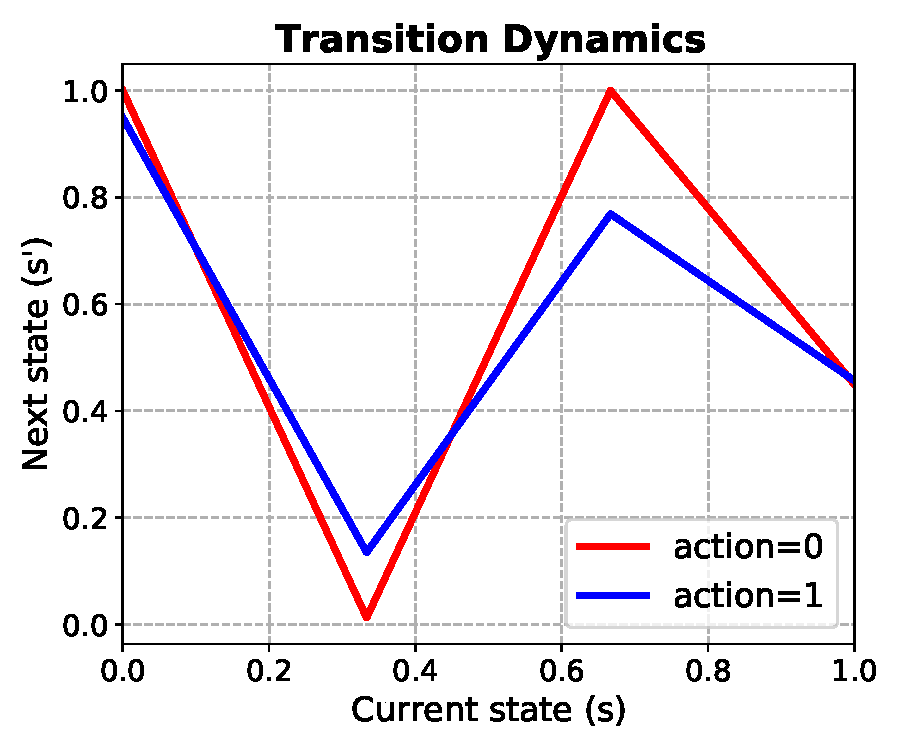
\includegraphics[width=0.48\linewidth]{section3_figs/dynamics.pdf}
    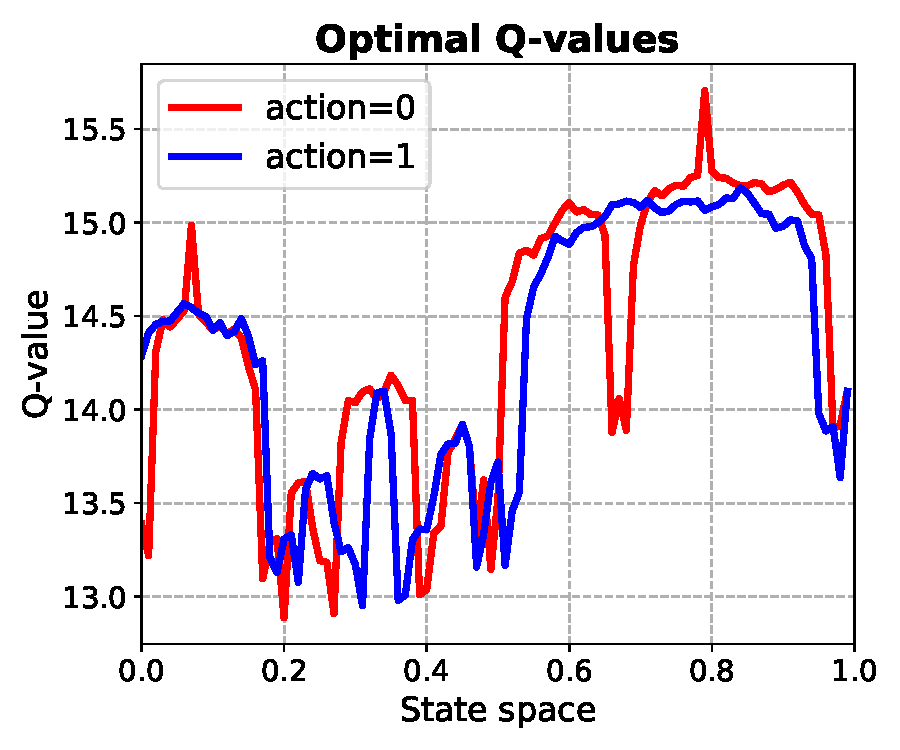
\includegraphics[width=0.48\linewidth]{section3_figs/optimal_q.pdf}
    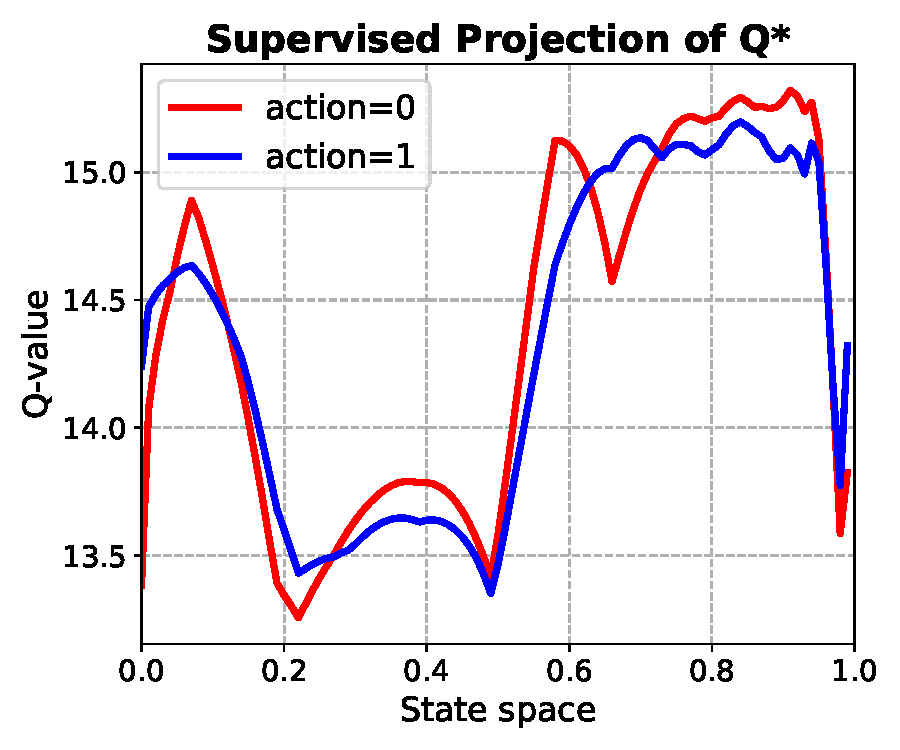
\includegraphics[width=0.48\linewidth]{section3_figs/supervised_q.pdf}
    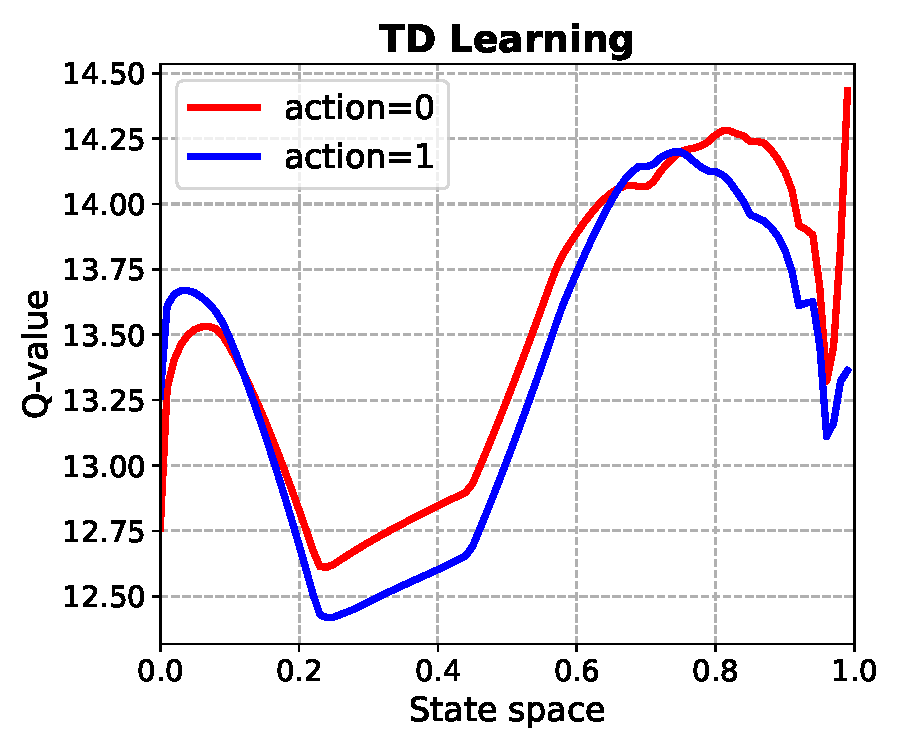
\includegraphics[width=0.48\linewidth]{section3_figs/td_learning.pdf}
    \vspace{-0.21cm}
    \caption{\small{\textbf{TD-learning fails to represent high frequency changes in Q-functions much more than supervised learning.} On the 1D MDP (dynamics, top-left), TD learning ignores the high-frequency components of the Q-function leading to worse action selection compared to supervised regression.}} 
    \label{fig:1d_mdp}
    \vspace{-0.6cm}
\end{wrapfigure}
%%AK: Tengyu had an interesting suggestion here: represent the action choices of each function via a shaded interval on the the number line, using blue for a_0 and red for a_1. The number of switches will determine the complexity of the Q-function, and this will show that TD has 4 switches, supervised has 8 and actual has 12 or 13 switches.
\textbf{Inability to model high-frequency components of Q-function.} Prior work has noted that Q-functions can be highly non-smooth even when reward functions and dynamics are relatively simple~\citep{dong2020expressivity}.
%%AK: does gamma models also note something related to complexity of Q vs reward via the discount profile stuff?
Would feature co-adaptation lead the Q-function to ignore certain high-frequency components in the objective?
As a didactic example of this phenomenon, we utilize a 2-action MDP with a 1-D state space $\mathcal{S} \in [0, 1]$ from~\citep{dong2020expressivity}. This MDP exhibits a piecewise linear dynamics (Fig.~\ref{fig:1d_mdp}, top-left) and an identity reward function $r(\bs, \ba) = \bs$ with two actions $\ba \in \{0, 1\}$. The optimal Q-function exhibits high-frequency changes (Fig.~\ref{fig:1d_mdp}, top-right). We find that running Q-learning (Fig.~\ref{fig:1d_mdp}, bottom-right)
attains Q-functions that completely ignore these high-frequency changes. This often makes the resulting policy choose the worse action of the two possible actions. On the contrary, a supervised projection (Fig.~\ref{fig:1d_mdp}, bottom-left) of the Q-function does capture many of these high frequency shifts in the Q-function. To formalize this didactic example, we prove the following result showing that high-frequency components of the Q-function are not modelled as a direct consequence of Theorem~\ref{thm:aliasing_exists}. The proof and a complete statement for Theorem~\ref{thm:num_pieces} can be found in Appendix ??.

%%AK: this will have some conditions on dynamics too, maybe we mention that as a detail in the appendix? But if it is unclear, maybe we should add it here, and explain it here...
\begin{theorem}[Informal]
Assume that the state-space $\mathcal{S}$ of the MDP is given by the 1-D number line, and that the groundtruth Q-function is (approximately) piecewise linear in the state $s$ with $N^*$ pieces. Denote the (approximate) number of linear pieces in a learned infinite-capacity ReLU Q-network via direct supervised regression as $N_{\mathrm{Sup}}$ and via TD-learning as $N_{\mathrm{TD}}$. Then: $N_{\mathrm{TD}} \leq N_{\mathrm{Sup}} \leq N^*$.     
\label{thm:num_pieces}
\end{theorem}
%%AK: In the proof of this theorem, we show this for approximate number of pieces, which is the integral of the second derivative of the function w.rt.t the input over the input space, but I think going into details would just hurt understanding here.

%%AK: I am a little unsure about the following part, in the sense if we should have it or not? This might seem obvious to some extent? 
% \textbf{Severe co-adaptation renders distributional shift corrections ineffective.} To test whether offline RL corrections alleviate feature co-adaptation, we performed a controlled experiment -- we constrained offline RL regularizers to only control the last linear layer of the Q-network, whereas bootstrapping was allowed to train the entire network. While we might expect that offline RL methods may still be effective by adapting the last weight layer to the features, contrary to this expectation, as shown in Figure ??, we find that all such variants (denoted as CQL($\phi$)) perform extremely poorly compared to the complete offline RL method. Further note the inability to minimize the regularizer corresponding to distributional shift and an increased dot-product similarity, $\Delta(\bs, \ba, \bs', \ba')$. This indicates that feature co-adaptation can lead to failure of offline RL methods. \textcolor{red}{add new figure for this}
%%AK: If we do keep this, maybe we should also add some line to justify why offline RL methods are still sensitive -- this is because they are not exactly doing SARSA?

\textbf{Lack of stability near ``good'' Q-function solutions.}
%%SL.5.22: instead of using a vague term like "good" with scare quotes, can we just say optimal? And what does "lack of stability" mean? Maybe just state it directly: Implicit regularization can prevent convergence, even when initializing at an optimal solution. [or something like that]
Finally, we study if co-adaptation of features cause the TD-learning process to diverge away, even when initialized favorably in the vicinity of a good Q-function (e.g., one obtained via supervised regression to MC returns or one obtained via online RL). Running Q-learning from such a favorable initialization eventually produces solutions that perform poorly as shown in Figure ?? below. Moreover, \textcolor{red}{say something about ranks here}. Indeed, in accordance with Theorem~\ref{thm:aliasing_exists}, the feature co-adaption phenomenon drives learning towards solutions with lower $\srank(\bM_{\mathrm{TD}}(\phi))$ values, giving rise to poor performance. \textcolor{red}{add figure, theorem}      
\fi

%%SL.5.17: what are Bellman constraints?
% are only enforced approximately (i.e., when the TD error
% %%SL.5.17: was the TD error ever defined?
% is not exactly 0), the implicit regularization towards minimum $||\bw||_2$ norm solutions will lead to the Q-function ignoring high-frequency components. That is, if the true Q-function changes dramatically from one state to the next, low TD-error solutions will fail to represent these changes.
%%SL.5.17: I don't see why the above theorem indicates that this is true
%%AK: add a worst-case theorem as discussed with George today?
%%SL.5.17: maybe we should put this didactic example into a separate \paragraph{} with more setup, instead of presenting this as a kind of footnote -- as-is, I think many people will not really understand it


%%AK: Check if we can take this paper's "peicewise linear theory" and convert it to a policy improvement bound differentiating between TD and supervised, as opposed to just fitting Q*-values?

% \subsection{Consequences of Overly Regularized Representations in TD Learning}
% Having seen aliasing of features on state-action tuples used for bootstrapping emerge as one pathological consequence of overly regularized representations in TD-learning compared to supervised learning, we next ask the following question we study the impact of over-regularization have on the performance of TD-learning. In particular, we ask: do TD-learning algorithms find generalizing and stable optima? To answer these questions, we consider a simple scenario where learning is initialized from a 


% \textbf{Abstract model.} Our abstract model captures feature learning as making a discrete selection among $K$ different feature vector candidates, $\{\Phi_1, \Phi_2, \cdots, \Phi_K\}$, $\Phi_i \in \mathbb{R}^{|\data|\times d}$,
%%SL.5.13: It would be way easier to understand if we could get continuous domains, and then just frame this as an optimization over \Phi (i.e., optimization over \Phi corresponds to selecting the best \Phi \in [some set]), that way we don't have to have this "discrete selection" business and could just say that it's part of the optimization process.
% and then training a linear layer $\bw \in \mathbb{R}^{d}$ to obtain the Q-function.
%%SL.5.13: One way you could phrase is this: Our abstract model of the learning process separates the neural network into two parts: a representation $\Phi$ and a weight vector $\bw \in ...$, such that the full model is given by $\Phi(..)^T \bw$ (i.e., $\bw$ corresponds to the last linear layer). The learning process is framed as a \emph{bilevel} optimization problem, where the weights $\bw$ are chosen subject to a constraint that the learning process chooses the optimal features $\Phi \in [set]$ for $\bw$ (or something like that)
% To mimic the overparameterized nature of neural networks, we assume that we operate in the overparameterized regime with $n < d$.
%%SL.5.13: This is kind of weird -- usually the last layer features are not that high dimensional, but the model parameters are. Are you sure we shouldn't look for some way to "NTK-ify" this? Perhaps a better way to frame this is that we are in the NTK regime where the choice of Phi corresponds to the choice of NTK (i.e., it's not fixed, as is more common in this analysis), while bw corresponds to the neural net parameters? That would justify the overparameterized regime and make this less weird.
% Assume that the initial value of the weight vector $\bw^{(0)} = 0$. We then write out the minimum-norm optimization problem shown below in Equation~\ref{eqn:min_norm} that attains the same solution as the optimal solution found by minimizing training TD error in this model, and characterize the properties of features $\Phi_K^*$ that are selected to obtain the minimum-norm solution. \textcolor{red}{more assumptions?}     
%%SL.5.13: It won't be clear to some people what min-norm has to do with neural net training, can you cite something to justify this?
% \begin{align}
%     \min_{\bw, \boldm_i \in \{0^d, 1^d \}}~~& ||\bw||_2^2 \nonumber\\
%     \text{s.t.}~~&~ \bar{\Phi}^\top \bar{\Phi} \bw = \bar{\Phi}^\top R + \gamma \bar{\Phi}^\top P^\pi \bar{\Phi} \bw, ~~ \bar{\Phi} = \left[\Phi_1, \cdots, \Phi_k\right] \otimes [\boldm_1, \cdots, \boldm_K]
% \label{eqn:min_norm}
% \end{align}
%%SL.5.13: ouch, this \bm_i is... difficult to parse
% Our first result characterizes the feature representation $\bar{\Phi}$ -- equal to one of $\Phi_i$ selected based on the learned masks $\bm_i$ -- that satisfies the Bellman consistency condition but also minimize the implicit regularizer, $||\bw||_2^2$,
% %%SL.5.13: where does this implicit regularizer come from?
% and use this to depict the existence of this phenomenon.


\iffalse

\section{Representation Regularization in Offline Q-Learning}
\label{sec:problem}
%%SL.5.13: See my comment on the title about "excessive" (maybe we call it Implicit Over-Regularization?). That said, this again sounds *extremely* similar to IUP, to the point where the section title alone could lead many readers to suspect this is just a direct copy of the IUP paper.
%%AK: yeah I agree. I am a little unsure what to call it, besides maybe admitting that this is similar IUP in high-level motivation but not low-level technical details. Do you think that's doable? My rationale was that right now readers might have the impression that we are trying to do something like IUP but also trying to distinguish it from IUP, without making clear what our contribution is and what's already there. Perhaps just saying something like "Fine-grained analysis" or something that explicitly quantifies the extent of this contribution is different? Avoiding that might just create questions. What do you think?
%%AK: the title sounds lika having a good connotation, is there a bad word for "regularization" that is not just "over-regularization" or "aliasing"?

% In this section, we study the mechanism by which implicit regularization effects are induced in offline Q-learning, and discuss how these effects can lead to pathological issues such as overly aliased representations and convergence to poor solutions. These aliasing properties exist even when learning is initialized from good solutions that do not exhibit this aliasing, and can make the learning eventually diverge. We first provide an empirical analysis of this phenomenon and then theoretically formalize these observations in a simple abstract model of learning dynamics of Q-learning.
Offline RL algorithms discussed previously are unstable and suffer from hyperparameter tuning challenges. A simple choice such as the number of training steps can be game-changing -- too few gradient steps will of course give rise to underfitted Q-functions, but perhaps surprisingly, too many gradient steps also lead to poor performance (Figure~\ref{fig:atari_5_percent}, Figure 2 in \citep{kumar2021implicit}). This phenomenon resembles statistical overfitting at first, however, it is actually underfitting caused due to excessive representational regularization of training deep networks with TD error that manifests as aliased features. While this issue has been broadly noted in previous work~\citep{kumar2021implicit}, in this section we will provide a fine-grained analysis of this phenomenon first empirically and then theoretically. In Section~\ref{sec:method}, we will then discuss a simple regularization scheme that can mitigate this issue. \textcolor{red}{TODO}  
%%SL.5.13: Maybe a somewhat more forceful lead-in could look like this:
% While the offline RL algorithms discussed in the previous section mitigate the worst challenges of offline RL~\citep{bear}, effectively using such methods in practice still requires extensive hyperparameter tuning. A particularly delicate choice is the number of gradient steps to take on the offline dataset -- too few gradient steps obviously produce underfitted, suboptimal value functions. But surprisingly, too many gradient steps also often result in poor performance, as illustrated in Figure ??. What is the reason for this performance collapse? While this phenomenon initially resembles overfitting, it is in fact an instance of \emph{underfitting}: although deep networks trained with SGD should provide a very good fit in standard supervised settings, we will argue that training with TD backups introduces a pathological over-regularization effect, induces excessive aliasing, and greatly constrains the expressive power of the resulting features. We first analyze this empirically, and then present a theoretical analysis. In Section ??, we will discuss how a simple regularization scheme can mitigate this issue.
%%AK: I havent added this fully, and instead cited IUP for the basic "noting" of this phenomenon and then said that we provide finegrained analysis of it. But I can change it. 

\iffalse
\subsection{Empirical Analysis}
\label{sec:empirical_analysis}
\begin{wrapfigure}{r}{0.49\textwidth}
    \vspace{-47pt}
    \centering
    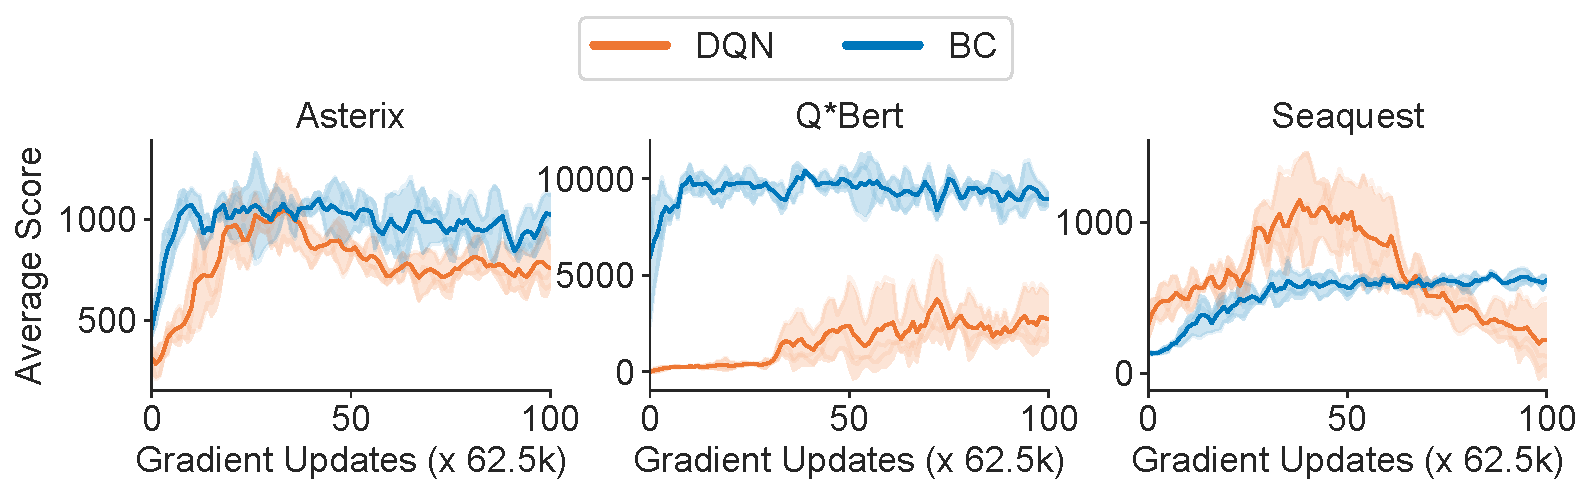
\includegraphics[width=\linewidth]{atari/perf_3_games.pdf}
    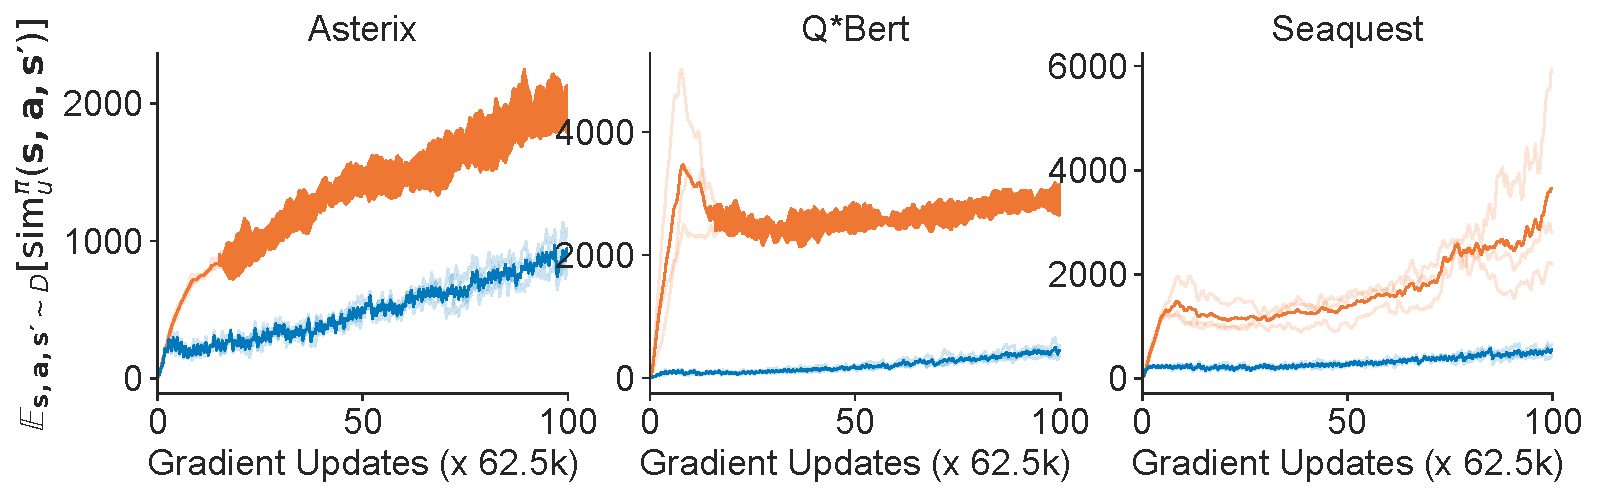
\includegraphics[width=\linewidth]{atari/unnorm_3_games.pdf}
    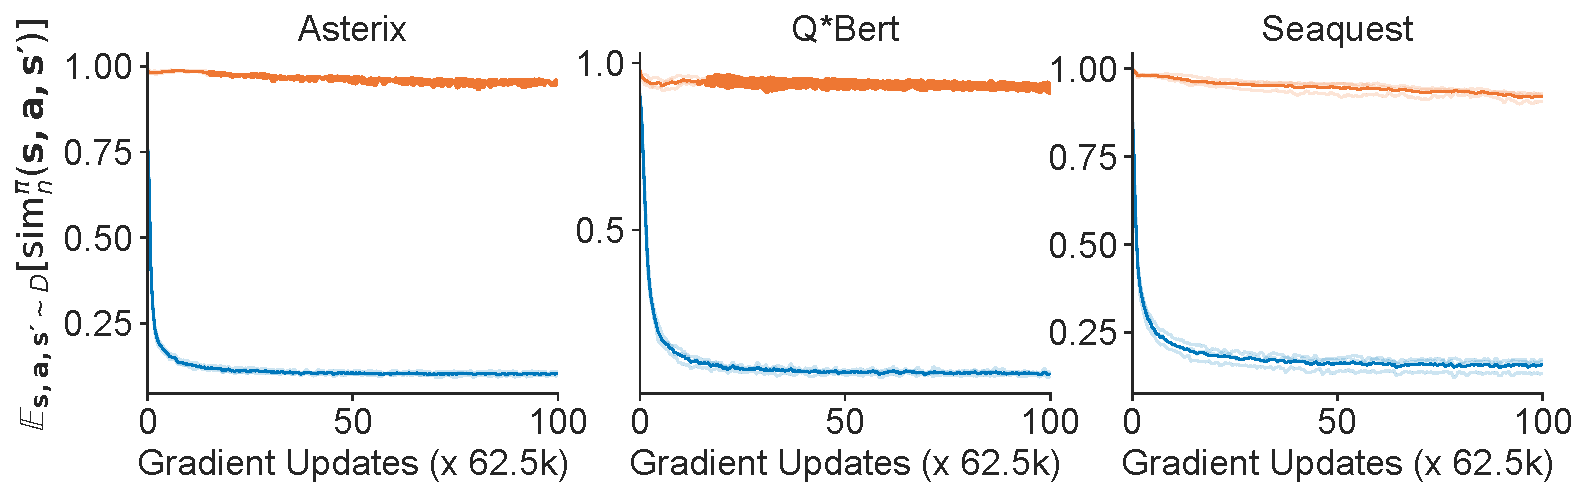
\includegraphics[width=\linewidth]{atari/norm_3_games.pdf}
    \vspace{-0.65cm}
    \caption{\small{Performance of offline DQN and BC on 5\% DQN replay dataset~\citep{agarwal2019optimistic} (top), normalized similarity scores for DQN and BC (bottom). As compared to DQN, $\simnorm$ (cosine similarity) decays significantly faster for BC. 
    \textcolor{red}{Remove the middle row that's not useful. Reduce to 2 games. Also add SARSA}}
    } 
    \label{fig:atari_3_games}
    \vspace{-0.4cm}
\end{wrapfigure}
%% The first para is saying aliasing exists in very simple language
%%SL.5.13: I think before we dive into why it happens, can we just show what the problem is? E.g., show some learning curves where performance peaks and drops, and explain what's going on. Only then talk about *why* it happens
%%AK: sorry for bringing this up again. But I feel like that would make it like iUP basically. I have cited this issue of what happens using a figure later in the paper in the para above as well as citing figure from IUP. We can put a wrapfig in the accompanying text above, but it feels a little copied if we spend the technical section on this. Maybe this is not a good choice. What do you think? 
As noted in~\citep{kumar2021implicit}, one of the most notably visible impacts of representation regularization is the pathological feature aliasing phenomenon that arises with more training. While this aliasing issue has been previously quantified via a collapse in the rank of the feature matrix $\Phi$, this evidence does not shed light on the exact mechanism by which aliasing happens -- even standard supervised learning would exhibit a drop in rank($\Phi$); though not in enormous amounts. % one closing line on how as a result it is less clear how to measure aliasing and connection to bootstrapping empirically.   
%%AK: tried to add a comparison against 

\textcolor{red}{This first part of Section 3.1 will likely be removed in favor of a didactic example} \textit{How can we connect the degree of aliasing to bootstrapping?} Since the difference between bootstrapping and standard supervised learning is primarily that the Q-function at $(\bs, \ba) \in \mathcal{D}$ is trained  with targets generated using Q-values at $(\bs', \ba')$ instead of fixed targets, excessive similarity between $\phi(\bs, \ba)$ and $\phi(\bs', \ba')$ leads to highly coupled Q-values on the two sides of the Bellman update, which can lead to issues such as overestimation and divergence~\citep{durugkar2018td}. Hence, it is informative to measure the similarities in representations $\phi(\bs, \ba)$ and $\phi(\bs', \ba')$. We measure two notions of similarity: \textbf{(1)} we measure the cosine similarity between $\phi(\bs, \ba)$ and $\phi(\bs', \ba')$, and \textbf{(2)} we measure an aggregate    

Observe in  Figure~\ref{fig:atari_3_games} that perhaps surprisingly the similarity between $\phi(\bs, \ba)$ and $\phi(\bs', \ba')$ decreases and saturates at low values with behavior cloning (BC),
%%SL.5.13: This feels like a non-sequitur -- you're comparing representations at two different states, why does it matter that BC is trying to match the behavior policy?
On the other hand, DQN, which is trying to actually improve upon the behavior policy, essentially aliases
%%SL.5.13: There is no evidence of aliasing, just of high dot product (which is not the same)
feature representations at $(\bs, \ba)$ and $(\bs, \ba')$, giving rise to very high similarity values.
%%SL.5.13: Without more context about what's going on, I would say at this point that this is probably due to the OOD actions problem you mentioned before, which DQN does nothing to fix. Additionally, I think it's very likely that many reviewers at this point woudl complain that it's non-sensical to compare BC (which learns policies) with DQN (which learns Q-functions).
This indicates that, compared to supervised learning (e.g., BC), implicit regularization effects in deep Q-learning have a tendency to alias predictions at states and corresponding next states. \textcolor{red}{Would be good to show this with SARSA vs MC: that way we can make a stronger statement like: Note that while both SARSA and MC returns are essentially computing the same quantity and differ only in the nature of implicit regularization induced. This difference makes a huge difference -- in one case, representations at consecutive states are essentially completely aliased, while supervised learning is able to disentangle representations.}
%%SL.5.13: Overall, I think this paragraph is rather problematic. If you want to explain this part, it would be good to really slow it way down and walk the reader through it much more slowly, otherwise so many of the choices in the above paragraph come across as ad hoc, making the conclusions unconvincing.

\fi

\subsection{A Didactic Example}
\label{sec:empirical_analysis}

As noted in~\citep{kumar2021implicit}, one of the most notably visible impacts of representation regularization is the pathological feature aliasing phenomenon that arises with more training. While this aliasing issue has been previously quantified via a collapse in the rank of the feature matrix $\Phi$, this evidence does not shed light on the exact mechanism by which aliasing happens -- even standard supervised learning would exhibit a drop in rank($\Phi$) with more training, and while prior work shows that bootstrapping exacerbates it empirically, it is unclear how exactly this amplification happens. In this section, we describe the intuition behind this mechanism with a didactic example of a 2-action, 1D line MDP~\citep{dong2020expressivity} with a piece-wise linear deterministic dynamics function, $P(\bs'|\bs, \ba) = \mathbb{I}(\bs' = f(\bs, \ba))$ shown in Figure ??. The reward $r(\bs, \ba)$ at any state is the value of the state itself, i.e., $r(\bs, \ba) = \bs$.

The optimal Q-function for this MDP is shown in Figure ??, and 3-layer deep ReLU network Q-functions estimators learned via supervised regression and TD-learning on the identical finite dataset are shown respectively in Figures ?? and ??. While neither supervised regression nor TD learning can learn the complete structure of the optimal Q-function, TD learning fails to represent important high-frequency components of the Q-function (marked in yellow), leaning a ``simple'', smooth Q-function. Since it fails to model the changes in the Q-function well, the resulting policy often chooses the worse action. Quantitatively, the policy extracted from such a TD Q-function is worse than that extracted from the supervised Q-function at more than half the states.  
%%AK: todo: mark in yellow via keynote

%% The next para is saying aliasing is undesirable
\textbf{Why do we observe overly smooth Q-functions in the didactic example when trained with TD learning?}  While excessive aliasing of internal representations in the neural network is expected to generally lead to poor performance, aliasing between $\phi(\bs, \ba)$ and $\phi(\bs', \ba')$ is especially detrimental when learning with Bellman backups. Intuitively, since Bellman backups train features such that the difference of Q-values, $Q(\bs, \ba) - \gamma Q(\bs', \ba')$ matches the reward function, $r(\bs, \ba)$, only on a finite number of state-action tuples seen in the dataset, the features $\phi(\bs, \ba)$ and $\phi(\bs', \ba')$ can learn to only be sufficiently different to predict the reward, thereby achieving low TD error and may be excessively regularized otherwise, thus not capturing long-term structure in the Q-function. Put in other words, there are many possible assignments of weights to a function approximator that could give rise to equally low TD error at the cost of varying degrees of aliasing or regularization.

%%SL.5.13: This feels really hand-wavy. I'm also not sure I agree with this argument -- after all, how would it be any different if there *wasn't* aliasing? Wouldn't you still get a good fit between the difference and reward? This kind of a makes a non-falsifiable statement.
%%AK: this figure is like the example in the MB vs MF paper, but with Bellman backups run on it.

\begin{wrapfigure}{r}{0.5\textwidth}
    \centering
    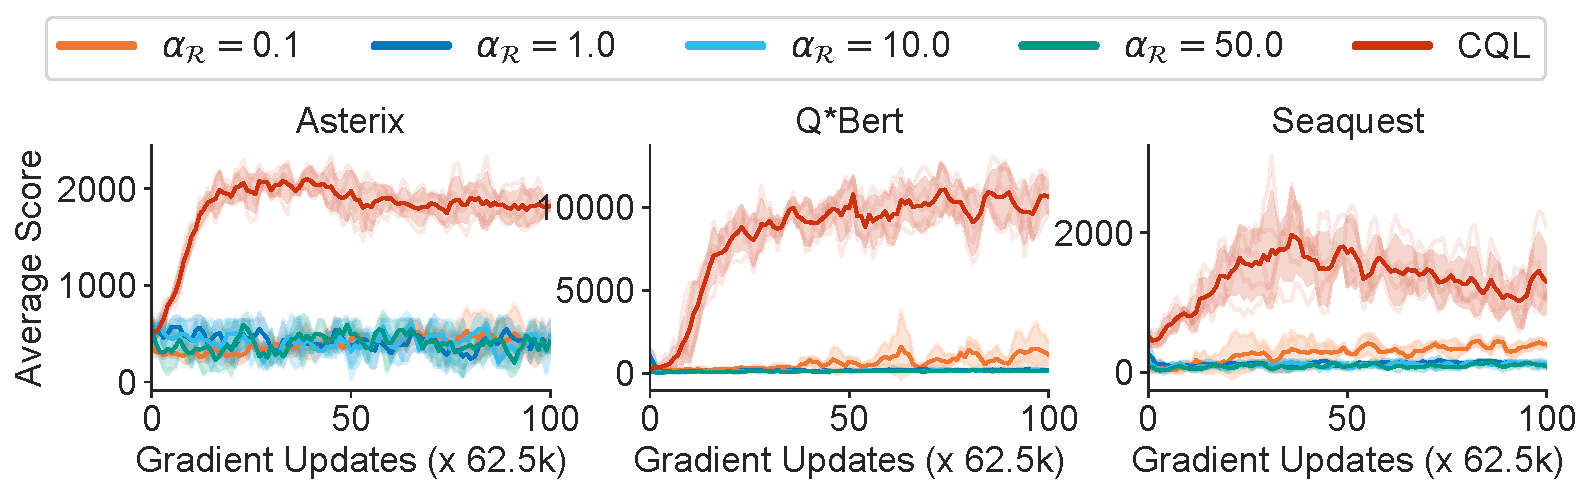
\includegraphics[width=\linewidth]{atari/cql_on_bootstrapping_feat.pdf}
    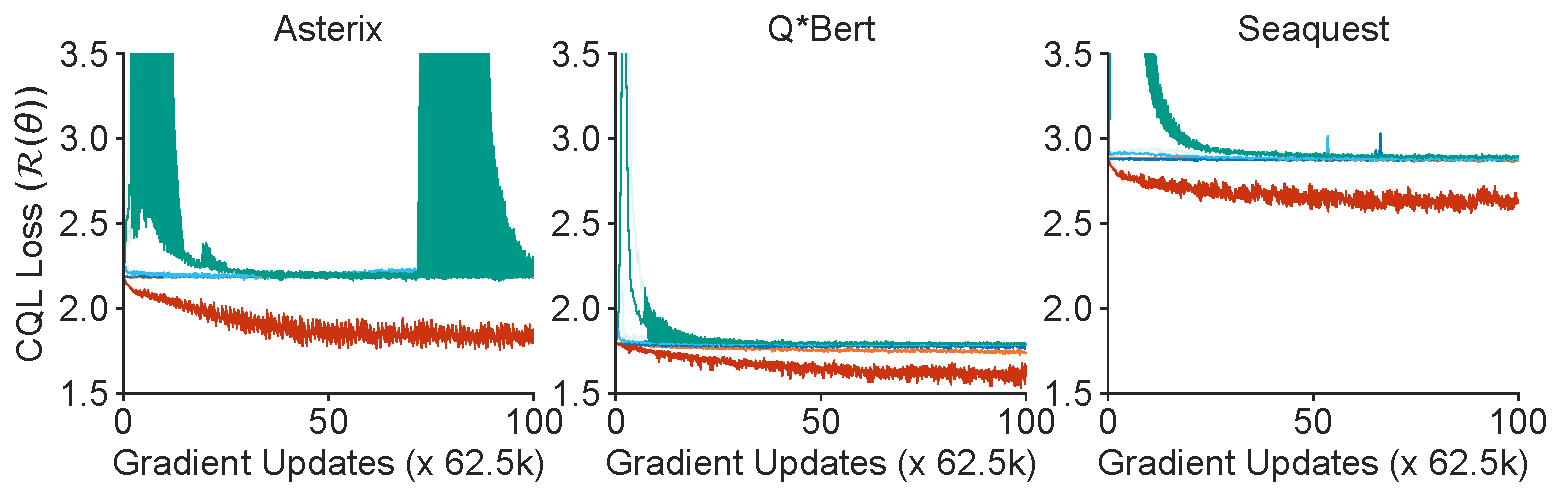
\includegraphics[width=\linewidth]{atari/cql_losses_bootstrapped_feat.pdf}
    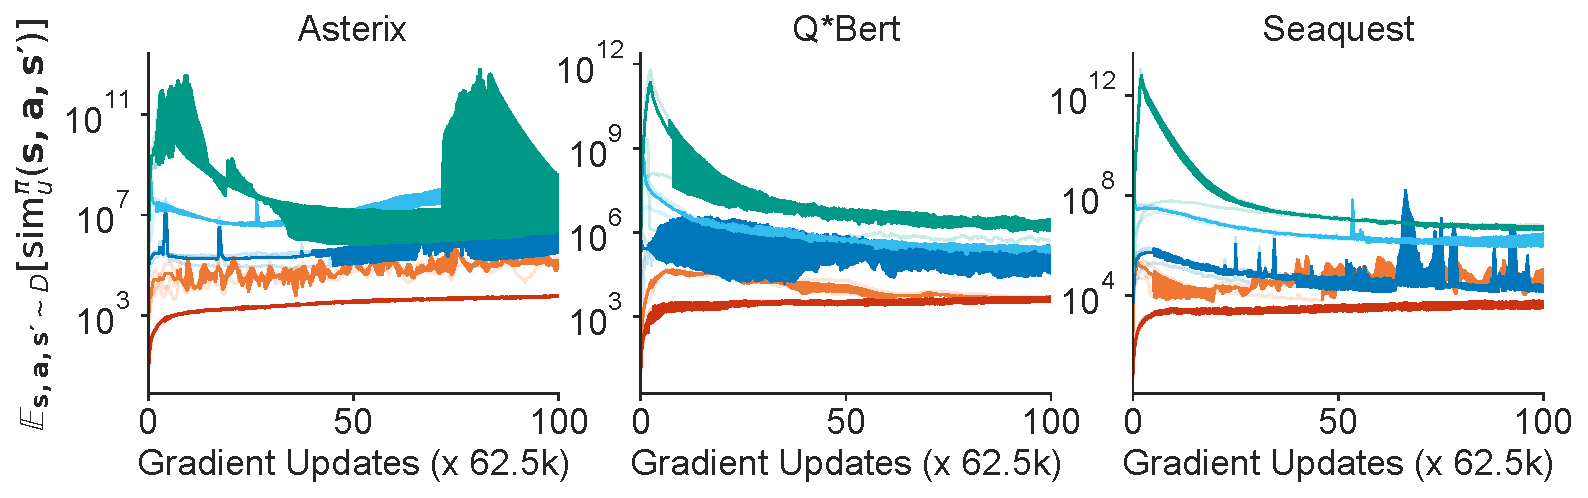
\includegraphics[width=\linewidth]{atari/sim_s_ns_cql_on_bootstrapping_feat.pdf}
    \vspace{-0.65cm}
    \caption{\small{CQL($\phi$), trained using 5\% DQN replay dataset, that learns on features trained solely via bootstrapping where the CQL regularizer $\mathcal{R}(\theta)$ only updates the linear weights of the Q-network. Different values of $\alpha_R$ correspond to different strengths of conservative regularization. We also show standard CQL~(red) for comparison.}} 
    \label{fig:atari_3_games_cql_bootstrap}
    \vspace{-0.6cm}
\end{wrapfigure}
When excessive aliasing is induced by such a mechanism, even modern offline RL methods that are meant to prevent against distributional shift
%%SL.5.13: It's unclear what preventing distributional shift has to do with this
are rendered ineffective. To demonstrate this empirically, we trained a modified version of CQL~\citep{kumar2020conservative}, CQL$(\phi)$, that learns on features $\phi(\bs, \ba)$ solely trained via bootstrapping, and the CQL regularizer is allowed to only update the last linear layer weights. As shown in Figure~\ref{fig:atari_3_games_cql_bootstrap}, no strength of conservative regularization is able to minimize out-of-distribution Q-values resulting in higher values of CQL loss and significantly worse performance as compared to CQL. This indicates that, no matter what, aliased representations can significantly hamper the efficacy of offline RL methods.
%%SL.5.13: This experiment seems weird. You said (and showed before) that features learned with bootstrapping are bad, and it seems like now you are saying if you take those features and retrain, it's still bad, but that's not surprising. I think the subtlety here is that you are also showing that the CQL regularizer is ineffective, but that seems obvious? And it also requires a degree of familiarity with CQL to understand, that the reader might not have. Maybe we can do away with this paragraph?

%%AK: this is the experiment where we initialize the Q-function from a good checkpoint and show it still performs poorly so it is reasoning about the stability aspect.
Finally, to demonstrate the detrimental extent of this implicit regularization on stability of the offline RL algorithm, we perform a controlled experiment where Q-learning is initialized from a ``good'' Q-function that doesn't exhibit aliasing.
%%SL.5.13: where does this come from?
As shown in Figure ??,
%%AK: TODO(AK): add figure!
more learning iterations with modern offline RL algorithms can still drive the algorithm away from this good solution towards more aliased and poor performing solutions. This shows that aliasing caused due to the implicit regularization of training does not just affect the peak performance of an algorithm, but also plays a significant role in destabilizing algorithms when they reach their peak performance.  

\subsection{Theoretical Analysis of Implicit Regularization in Offline Deep Q-Learning}
\label{sec:theory_evidence}
%%SL.5.13: Calling this "implicit regularization" seems premature -- all we showed is that features get larger dot products, which doesn't mean there is some sort of "implicit regularization" going on
In this section, we formalize our empirical observations from Section~\ref{sec:empirical_analysis} and provide a theoretical analysis of the implicit regularization issue. We aim to answer two questions: \textbf{(1)} How do implicit regularization effects in TD learning affect the the aliasing of representations at consecutive states used in the Bellman update? and, \textbf{(2)} How does excessive aliasing affect performance of the algorithm? To answer these questions, we first introduce a simple abstract model of neural network behavior
%%SL.5.13: Rephrase as something like: we first introduce a simple abstract model of neural network training dynamics in value-based RL, and then use this model to analyze the effect of repeated SGD updates on the TD objective. [or something like that]
that allows us to answer these questions.

% abstract model
%% AK: TODO (AK): Also check if we can generalize this to arbitrary continous domains
%%SL.5.13: In its current form, I'm a bit nervous about this version of the theory. I think the SGD implicit regularization version is more convincing and makes fewer arbitrary choices. I do think this version could be made better if we can get rid of the discrete set though. Would be good to get Tengyu's take on it too...
\textbf{Abstract model.} Our abstract model captures feature learning as making a discrete selection among $K$ different feature vector candidates, $\{\Phi_1, \Phi_2, \cdots, \Phi_K\}$, $\Phi_i \in \mathbb{R}^{|\data|\times d}$,
%%SL.5.13: It would be way easier to understand if we could get continuous domains, and then just frame this as an optimization over \Phi (i.e., optimization over \Phi corresponds to selecting the best \Phi \in [some set]), that way we don't have to have this "discrete selection" business and could just say that it's part of the optimization process.
and then training a linear layer $\bw \in \mathbb{R}^{d}$ to obtain the Q-function.
%%SL.5.13: One way you could phrase is this: Our abstract model of the learning process separates the neural network into two parts: a representation $\Phi$ and a weight vector $\bw \in ...$, such that the full model is given by $\Phi(..)^T \bw$ (i.e., $\bw$ corresponds to the last linear layer). The learning process is framed as a \emph{bilevel} optimization problem, where the weights $\bw$ are chosen subject to a constraint that the learning process chooses the optimal features $\Phi \in [set]$ for $\bw$ (or something like that)
To mimic the overparameterized nature of neural networks, we assume that we operate in the overparameterized regime with $n < d$.
%%SL.5.13: This is kind of weird -- usually the last layer features are not that high dimensional, but the model parameters are. Are you sure we shouldn't look for some way to "NTK-ify" this? Perhaps a better way to frame this is that we are in the NTK regime where the choice of Phi corresponds to the choice of NTK (i.e., it's not fixed, as is more common in this analysis), while bw corresponds to the neural net parameters? That would justify the overparameterized regime and make this less weird.
Assume that the initial value of the weight vector $\bw^{(0)} = 0$. We then write out the minimum-norm optimization problem shown below in Equation~\ref{eqn:min_norm} that attains the same solution as the optimal solution found by minimizing training TD error in this model, and characterize the properties of features $\Phi_K^*$ that are selected to obtain the minimum-norm solution. \textcolor{red}{more assumptions?}     
%%SL.5.13: It won't be clear to some people what min-norm has to do with neural net training, can you cite something to justify this?
\begin{align}
    \min_{\bw, \boldm_i \in \{0^d, 1^d \}}~~& ||\bw||_2^2 \nonumber\\
    \text{s.t.}~~&~ \bar{\Phi}^\top \bar{\Phi} \bw = \bar{\Phi}^\top R + \gamma \bar{\Phi}^\top P^\pi \bar{\Phi} \bw, ~~ \bar{\Phi} = \left[\Phi_1, \cdots, \Phi_k\right] \otimes [\boldm_1, \cdots, \boldm_K]
\label{eqn:min_norm}
\end{align}
%%SL.5.13: ouch, this \bm_i is... difficult to parse
Our first result characterizes the feature representation $\bar{\Phi}$ -- equal to one of $\Phi_i$ selected based on the learned masks $\bm_i$ -- that satisfies the Bellman consistency condition but also minimize the implicit regularizer, $||\bw||_2^2$,
%%SL.5.13: where does this implicit regularizer come from?
and use this to depict the existence of this phenomenon.

\begin{theorem}
\label{thm:aliasing_exists}
Let the singular value decomposition of $\Phi_i$ be given as $\Phi_i = \bU_i \Sigma_i \bV_i^\top$ and $\bw^{(*)}, \boldm^{(*)}$ minimize the objective in Equation~\ref{eqn:min_norm}. Assume that the reward vector lies in the column space of $\Phi_i$, $\forall i \in [K]$, i.e., $\exists~ y_i, R = \Phi_i y_i $.  Then, $\bar{\Phi}$ is such that:
\begin{equation*}
    \bar{\Phi} := \arg \min_{i}~ \big|\big| \Sigma_i^{-1} \left( \bU_i^T (I - \gamma P^\pi) \bU_i \right)^{-1} \Sigma_i y_i\big|\big|_2^2.
\end{equation*}
Thus, the resulting $\bar{\Phi}$ satisfies: $\mathrm{srank}\left(\bar{\Phi}^\top (\bar{\Phi} - \gamma P^\pi \bar{\Phi}) \right) \leq \mathrm{srank}\left(\Phi_i^\top (\Phi_i - \gamma P^\pi \Phi_i) \right)~ \forall i$, which quantifies the existence of aliasing between representations at consecutive states in TD-learning.
\end{theorem}
%%SL.5.13: It's not clear what this last sentence means ("which quantifies the existence of aliasing between representations at consecutive states in TD-learning") -- can we state the implication of this theorem more precisely. As written, it's also not clear what this theorem has to do with SGD (I guess it's the min-norm part?).

%%SL.5.13: It might also help with clarity to explain why this problem *doesn't* happen in the supervised learning case

A proof of Theorem~\ref{thm:aliasing_exists} can be found in the Appendix ??. The main consequence of this result is a characterization of the learned features at optimal TD solutions in our abstract model in terms of the effective rank~\citep{kumar2021implicit} of the matrix $\bM(\Phi) := \Phi^\top (\Phi - \gamma P^\pi \Phi)$. A low rank of $\bM(\Phi)$ for a given rank of $\Phi$ intuitively indicates that the basis of the difference in features at consecutive states, $\Phi - \gamma P^\pi \Phi$, heavily lies
%%SL.5.13: try to avoid hand-wavy language ("heavily lies") and state what you mean more precisely
in the null space of the feature matrix $\Phi$, as a result of which the weight vector $\bw$ will be updated only in a few directions allowed by both $\Phi$ and $\Phi-\gamma P^\pi \Phi$.indicating that only a partial set of features will actually be used for learning.
%%SL.5.13: something is malformed above ("indicating that")
To empirically verify the existence of such an aliasing phenomenon, following the procedure outlined in \citep{kumar2021implicit}, we measure the effective rank of $\bM(\Phi)$ and observe in Figure ?? that this matrix indeed has extremely low rank when training with TD backups, as compared to supervised regression.
%% AK: this supervised regression is BC. Should we also do this for something else?

%%AK: maybe write the stuff below as a theorem?
Another interesting consequence of Theorem~\ref{thm:aliasing_exists} is the effect of the ``simplicity'' of the reward function on feature aliasing. We define simplicity by the number of non-zero components in the vector $y_i$.
%%SL.5.13: maybe we should avoid ad hoc definitions like this, and try to just state this more plainly and directly?
As an extreme case, note that if the vector $y_i$ has all zeros, except a single 1 entry, the optimal $\bar{\Phi}$ is expected to induce $\bM(\Phi)$ with a much lower rank compared to when a significantly more number of values of $y_i$ are non-zero (as shown in Appendix ??).
%%SL.5.13: this seems imprecise ("much lower")
This means that when the reward function $R$ actually non-trivially combines the singular vectors of $\Phi$ -- which we refer to as a ``complex'' reward function -- the effective aliasing
%%SL.5.13: I think if you're going to use the term "aliasing" like this, it needs to be formally defined. Aliasing means that two things are indistinguishable (not similar, but indistinguishable). The word is being used in a different way here.
is little less than when it does not. We indeed observe this behavior in practice, as shown in Figure ?? in Section~\ref{sec:empirical_analysis}, and our abstract model sheds light on how this implicit regularization effect in TD-learning is exacerbated in scenarios where reward functions can be expressed using very few components of the feature matrix $\Phi$.
%%SL.5.13: how do you know if it can be expressed using very few components?
%%SL.5.13: I think I understand what you are trying to say in the above paragraph, but we need to find a cleaner and more concise way of saying it. Maybe what we can say is something like -- consider the projection of the reward function onto the column-space [?] of Phi, with coefficients ??. If these coefficients are sparse, we would expect [??] (try to be precise!)...

To conclude our analysis for question \textbf{(1)}, we finally note that an analogous result in supervised learning would indicate no existence of any implicit bias that preferentially aliases feature representations at consecutive states. While prior work \citep{kumar2021implicit} has also generally shown the compounding effect of implicit regularization towards low-rank $\Phi$ in TD-learning, our analysis explicitly identifies the structure of aliasing induced by this implicit regularization: the rank of the matrix $\bM(\phi)$ drops, leading to aliasing at consecutive states.
%%SL.5.13: It's good to have a paragraph like the one above, but it addresses two things simultaneously, and doesn't do either very well: the supervised learning bit seems to have no punchline (so... is this a contradiction? if not, why not?); the bit about IUP doesn't clearly state how what you are showing is different from IUP.

%%SL.5.13: Given how long-winded the above is, maybe consider a subsection heading for (2) or something (or at least paragraph heading)
Next, we answer question \textbf{(2)} regarding the detrimental impacts of aliasing. 
\textcolor{red}{Need to finish this bit -- there are some options we can go: (1) We can show that there exist MDPs with simple reward functions and complex Q-functions, where such an implicit regularizer will cause the MDP to learn overly smooth Q-functions. (2) We can show that even when initialized close to a good solution, this implicit regularizer will drive the model towards picking features that are the most aliased, in which case we do not even stabilize near a good solution even if we reach it. (3) We could show that distributional shift correction on top of aliased features will not work, similar to what we had before the ICML deadline. Which of these option(s) should we prefer?}

\fi






















%%%%%%%%%%%%%%%%%%%%%%%%%%%%%%%%%%%%%%%%%%%%%%%%%%%%%%%%%%%%%%%%%%%%%%%%%%%%%%%%
%%%%%%%%%%%%%%%% old stuff below %%%%%%%%%%%%%%%%%%

\iffalse
\section{\AliasingProblemName\ in Offline RL}
\label{sec:problem}
%%SL.2.3: Kind of a nitpick, but "Bootstrapping Aliasing" kind of makes it sound like we are bootstrapping the aliasing (rather than that we have aliasing that stems from bootstrapping). But why do you want "bootstrapping" in the name? It doesn't really have anything to do with bootstrapping, at least not moreso than anything else that relates to RL. It's kind of more like Policy Aliasing (or something like that...)

Empirically, we find that the combination of neural network function approximators, bootstrapping, and minimizing TD error 
% with gradient descent 
leads to aliasing
%%SL.2.3: Aliasing between what and what?
of the state-action pairs appearing in a Bellman update. Minimizing TD error against bootstrapped targets uses a tuple $(\bs, \ba, \bs')$ from the dataset, draws an additional action sample from $\pi(\cdot | \bs')$, which may not be observed in the dataset, and evaluates $Q_\theta(\bs, \ba)$ and $Q_\theta(\bs', \ba')$. We find that the features $\phi(\bs, \ba)$ and features $\phi(\bs', \ba')$ become aliased over the course of learning,
%In this section, we will see how offline training of Q-functions by minimizing TD error against a bootstrapped target value estimate \emph{aliases} feature representations on actions drawn from the dataset $\phi(\bs, \ba)$ and the feature representations on actions from the learned policy that will be used for bootstrapping, but are not observed in the dataset, which we denote as $\phi(\bs', \ba')$. Since features $\phi(\bs', \ba')$ directly influence the features at dataset state-action tuples $\phi(\bs, \ba)$ via the bootstrapping update, a similarity between features at these specific state-action tuples is likely to affect optimization dynamics of the algorithm as we will more formally discuss in Proposition~\ref{thm:separability}.  
%%AK.2.3: I don't know how to motivate this, I wrote something up but this isnt convincing 
%%SL.2.1: which we denote as
and we refer to this phenomenon as \emph{\aliasingproblemname}.
%%SL.2.3: As stated, this sounds a little bit silly, because \bs and \bs' are very similar, so of course they are likely to be aliased! I think it would help to explain the *policy* aliasing part first, and then explain that a particularly prominent instance of this has to do with \ba and \ba' (but FWIW, I still think we are making too big of a deal out of the fact that these are sequential actions, and things would be much clearer and less likely to be misunderstood if we did not do this, and instead focused on policy aliasing and brought in the s/a/s'/a' stuff as late as possible)
To measure this aliasing, we use the normalized and unnormalized dot product similarities %To begin, we formally define two metrics to quantify \aliasingproblemname, and then demonstrate the existence of this issue in offline Q-learning methods.
\begin{align*}
    \simnorm(\bs, \ba, \bs'; \phi) &:= \frac{|\phi(\bs, \ba)^T \E_{\pi(\ba'|\bs')}[\phi(\bs', \ba')]|}{||\phi(\bs, \ba)||_2 ||\E_{\pi(\ba'|\bs')}[\phi(\bs', \ba')]||_2},\\
    \simunnorm(\bs, \ba, \bs'; \phi) &:= |\phi(\bs, \ba)^T \E_{\pi(\ba'|\bs')}[\phi(\bs', \ba')]|.
\end{align*}
%\begin{definition}
%\emph{\Aliasingproblemname} is said to happen when features $\phi(\bs, \ba)$ on $(\bs, \ba, \bs') \in \data$ and the expected feature vector on actions drawn from the learned policy $\pi(\cdot |\bs')$ at the next state $\bs'$, $\E_{\ba' \sim \pi(\cdot|s')}[\phi(\bs', \ba')]$, exhibit a high normalized or unnormalized dot product similarity on an average over the dataset $\mathcal{D}$. The normalized ($\simnorm$) and unnormalized ($\simunnorm$) similarities are given by:
%%%SL.2.1: It's unclear why you are using a/a' on successive timesteps. Since this is a definition, it might come across as weirdly arbitrary. Beyond this, there is the question of whether this is referring to this quantity in expectation over s, on average, etc.
%%%AK.2.3: I don't know how best to do that. I want to write this section as policy indistinguishability, where we measure (s, a), (s, a') similarity, but that doesn't seem to be the case we can make in time
%\begin{align*}
%    \simnorm(\bs, \ba, \bs'; \phi) &:= \frac{|\phi(\bs, \ba)^T \E_{\pi}[\phi(\bs', \cdot)]|}{||\phi(\bs, \ba)||_2 ||\E_{\pi}[\phi(\bs', \cdot)]||_2},\\
%    \simunnorm(\bs, \ba, \bs'; \phi) &:= |\phi(\bs, \ba)^T \E_{\pi}[\phi(\bs', \cdot)]|.
%\end{align*}
%\end{definition}
We omit $\phi$ when it is clear from context. %A high $\simnorm$ indicates state-action tuples $(\bs, \ba) \sim \mathcal{D}$ and the next state-action tuple, $(\bs', \ba')$ where $\ba' \sim \pi(\cdot|\bs')$ are directionally aligned,
%%SL.2.1: Above sentence appears to (intentionally?) omit saying what the state is, just saying the action. Especially combined with the s/s'/a/s' confusion in the previous definition, this might be not so great
%%AK.2.3: added this 
%whereas the feature magnitude captured in $\simunnorm$ indicates the extent to which directional similarity affects optimization~(Section~\ref{sec:analysis}). As a result, by tracking average similarities over the dataset, $\E_{\bs,\ba, \bs' \sim \data}[\simnorm(\bs, \ba, \bs')]$ and $\E_{\bs, \ba, \bs' \sim \data}[\simunnorm(\bs, \ba, \bs')]$,
%%SL.2.1: This average thing seems a bit hacky.
%%AK.2.3: introduced the average bit in the definition above
%we can verify the existence of \aliasingproblemname.
Intuitively, this could be problematic in the offline RL setting where carefully controlling generalization is critical to performance~\citep{levine2020offline}
%%SL.2.3: I don't really understand what claim this reference is supposed to be supporting
because it couples the $Q$ values of $(\bs, \ba)$ and a potentially out-of-distribution tuple $(\bs', \ba')$.
%%SL.2.3: should clarify that it's the action that's OOD, not the state (lest someone misunderstand)
% For example, assume that the features $\phi(\bs, \ba) \in \mathbb{R}^d$ are positive (as is the case with ReLU activations) and unit norm, then $\simnorm(\bs, \ba, \bs') \geq 1 - \varepsilon$ immediately implies that $(Q_\bw(\bs, \ba) - \E_{\pi(\ba'|\bs')}\left[Q_\bw(\bs', \ba')\right])^2 \leq 2\varepsilon||\bw||_2^2$.
%%SL.2.3: This early in the paper, the significance of this inequality is not clear (indeed, it's not clear to me even, and I've read the whole paper many times!)
In the next subsections, we present empirical evidence demonstrating that bootstrapping induces \aliasingproblemname\ and then discuss its consequences, before using these insights to develop \methodname\ in Section~\ref{sec:method}.  

%%SL.2.1: Overall, I'm concerned that there are a number of details in this section that make what would otherwise be a fairly clean exposition kind of confusing. Namely, the fact that there are two similarity measures, and the s/a/s'/a' thing. Perhaps in the interest of clarity we can simplify this? Not sure how well that would still fit with what follows later, but it seems like something we can do better. Beyond this, it's not clear why high "indistinguishability" is actually "indistinguishable" -- if the features are perfectly aligned, of course they are indistinguishable, but I do think that many readers will have the same criticism here that I had -- if the similarity is high but not perfect, then the features really are distinguishable, just the differences are smaller. We probably don't have room to do this concept justice in this section, but at least providing a little bit of intuition and/or a forward reference about it here would I think help.
%%AK.2.3: I edited this, does it seem better?


%%AK.1.31: discuss IUP in the related work section, TODO!
\subsection{High \AliasingProblemName\ During Training}
\label{sec:bootstrapping_evidence}
To study how $\simunnorm$ and $\simnorm$ evolve over the course of training with offline RL, we measure both quantities during training on three Atari games in \Figref{fig:atari_3_games}.
On each game, we run standard DQN~\citep{Mnih2015} on an offline dataset that consists of partially subsampled experience from an online Atari agent~\citep{agarwal2019optimistic}. For comparison, we visualize the corresponding metrics for supervised learning behavioral cloning and offline SARSA~\citep{rummery1994line} that uses the actions from the dataset at the next state for bootstrapping updates. First, note that both $\simnorm$ and $\simunnorm$ are an order of magnitude higher for DQN, as compared to supervised BC, \emph{despite the fact that BC is trying to directly match the behavior policy}, whereas DQN is trying to improve upon the behavior policy and intuitively representing the behavior policy from the learned policy is crucial for improvement. Furthermore, since there are no out-of-distribution actions used in SARSA, the \aliasingproblemname\ is more severe in DQN compared to SARSA.
%%SL.2.1: \emph{despite the fact that BC is directly trying to match the behavior policy}, while DQN is trying to improve on it
%%RA.2.2: I didn't understand why "despite" the fact -- do we expect BC's similarities to be higher?
%%AK.2.3: added the intuition
As compared to DQN, $\simunnorm(\bs, \ba, \bs')$ increases much slower for BC and SARSA while $\simunnorm(\bs, \ba, \bs')$ decays significantly faster for BC and SARSA.
%Note that these values also generally exhibit an increasing trend with DQN, but a relatively stable trend over more training for BC.
Furthermore, we observe a similar trend of large $\simunnorm$ and $\simnorm$~(\Figref{fig:atari_3_cosine}) during training for offline RL algorithms that address distributional shift, such as CQL~\citep{kumar2020conservative} and REM~\citep{agarwal2019optimistic}. Based on this evidence, we ask: 
%RA.2.3: Does the \aliasingproblemname\ issue happen consistently, or is this merely an accident? 
what are the consequences of \aliasingproblemname\ on algorithm performance? 
%RA.2.3: We will show in Section~\ref{sec:analysis} that bootstrapping combined with gradient descent indeed amplifies these similarity metrics, particularly $\simunnorm$.

%%AK.1.31: reword/remove the para below, if we actually arent able to show something from the min-norm problem.

% Can we improve performance by addressing this issue? 
%We investigate this question in the next section, and then propose \methodname\ that mitigates \aliasingproblemname\ and leads to more effective offline RL in practice.

%%SL.2.3: When we shuffles things around in the paper, I think we might have removed something from this section, because as written, it doesn't actually motivate anything significant: it just says this mysterious quantity we defined (and that we decided to call "aliasing") is higher for some methods than others. But right now, as far as I could tell, this section doesn't actually say anything about how this is *bad*. That seems like a problem, because the reader will probably think that we're just saying random stuff in this section, and might simply stop reading.



\subsection{Consequences of High \AliasingProblemName}
\label{sec:consequences_of_feature_sim}
%In this section, %we discuss the consequence of high feature similarity on the performance of offline RL algorithms. 
%we analyze the behavior of offline Q-learning when \aliasingproblemname ~is high.
%%%SL.2.1: I don't get this last part -- why does it correct for it "when $\simnorm$ and $\simunnorm$ are high"?
%%%RA.2.1: The previous sentence was confusing, what we mean is that the analysis is done when feature similarities are high.
%Our intuition is that with high similarities, the Q-function is unable to distinguish between dataset and out-of-distribution actions or it needs to learn high magnitude values in order to meaningfully distinguish between them, in which case it can no more a valid Q-function for the MDP (that takes on possible values for expected return in the MDP). 
%As a theoretical abstraction, we show in Theorem~\ref{thm:separability} that for a given offline dataset $\data$, %of size $|\data| = n$, 
%the probability of a large margin between the Q-values at  $(s, a) \sim \data$ and $(s, a) \sim \data, \pi$
%%%SL.2.1: As before, it seems like here there is a bit of cleverness in omitting which state this depends on -- but that detail is important. Of course actions at different states will have different representations...
%%%AK.2.3: addressed
%computed via a linear transformation on the features decreases with normalized similarities $\simnorm$.
%This implies that a valid Q-function  learned by any offline RL algorithm, even when it corrects for distributional shift, will not be able to push down the values of out-of-distribution actions by a large margin.
%%%SL.2.1: I'm not really sold on this statement. Is there a reason to believe that a numerically smaller margin implies that it is harder to distinguish things? Just scaling down the features by a constant factor as I had mentioned before would also have this property, but of course we wouldn't argue that this makes it any harder...
%%%AK.2.1: I edited this above to make it clear we are talking about the Q-function and not the margins of the representations independently. In a setting when I can drive the linear weights to infinity, the margin will be high, but here we can't as we will not have a valid Q-function at that point, and we will have ignored the reward maximization part. 
%% This induces brittleness~\citep{bellemare2016increasing}
%% %%SL.2.1: brittleness?
%% in the learning procedure, and stochasticity and randomness in optimization can lead to issues such as excessive overestimation~\citep{kumar2020conservative} and policy unlearning~\citep{levine2020offline}.
%%%SL.2.1: I would make the second clause (, and...) be a separate sentence, and explain it more explicitly -- are you trying to say that when \simnorm is high, stochasticity in optimization can lead to issues? or something else? it's just a pretty complex phrase to parse
%%%AK.2.3: removed this
%% We first state the result and then empirically validate it.
%\begin{proposition}
%\label{thm:separability}
%Assume that features $\phi(\bs, \ba) \in \mathbb{R}^d$ of the Q-function are uniform random vectors satisfying $\forall~ \bs, \ba, \bs' \in \data,~ ||\phi(\bs, \ba)||_2 = 1,\ \mathrm{and}\ \simunnorm(\bs, \ba, \bs') = \simnorm(\bs, \ba, \bs') \geq \sqrt{1 - \varepsilon^2}$. Let $f_{\bw_c}(\bs, \ba) = \bw_c^T \phi(\bs, \ba)$ be any linear classifier that separates $\data_{\mathrm{in}} = \{(\bs, \ba)\}$ and $\data_{\mathrm{OOD}} = \{(\bs', \ba')\}$, where $\ba' \sim \pi(\cdot|\bs')$. Let $\zeta$ denote the margin obtained by $f_{\bw_c}$ in classifying $\data_{\mathrm{in}}, \data_{\mathrm{OOD}}$, and  assume that classifier weights are bounded, $||\bw_c||_2 \leq \tau$.
%Then, 
%\begin{equation*}
%    \text{Pr} \left(\zeta \geq \alpha \right) \leq \left[ 1 - \left( C_1 \frac{\alpha^2}{\varepsilon^2}\right)^{\frac{d-1}{2}} \right]^{|\mathcal{D}|},
%\end{equation*}
%for some universal constant $C_1 > 0$ that depends on $\tau$.  
%\end{proposition}
%%%SL.2.1: What is the logic for why a small margin makes things bad? We can get a small margin just by making the features small (e.g., dividing them by 1000000), but this clearly wouldn't make the learning problem harder. More generally, I don't think we've really provided the setup that the reader needs to understand why separation between OOD and dataset actions is actually important. Maybe it's more important to establish that?
%%%AK.2.1: I edited this above to make it clear we are talking about the Q-function and not the margins of the representations independently. In a setting when I can drive the linear weights to infinity, the margin will be high, but here we can't as we will not have a valid Q-function at that point, and we will have ignored the reward maximization part. 
%Proposition~\ref{thm:separability} shows that when features are highly similar, \ie small $\varepsilon$, obtaining a Q-function that guarantees a large margin is exponentially smaller than when $\varepsilon$ is large. The proof for Proposition~\ref{thm:separability} can be found in Appendix ??. 
%%%SL.2.1: Why does it show that? I guess your intuition is that if in-distribution and OOD actions are close together, this is hard, but this is not at all obvious
%%AK.2.3: TODO (aviral): put a probability of divergence or something like that

To explore the consequences of \aliasingproblemname, we show that recent methods developed to mitigate the impact of \emph{distributional shift}, such as CQL~\citep{kumar2020conservative}, are ineffective when using features with high \aliasingproblemname. In particular, we evaluate a modified version of CQL, CQL($\phi$), that learns on features $\phi(\bs, \ba)$ trained solely via bootstrapping,
%%SL.2.3: Can you just show basic results first before modifying the method? and can you show things for methods other than cql? eg that regular DQN has high aliasing?
where the CQL regularizer only updates the last linear weight layer of the Q-network~(\Figref{fig:atari_3_games_cql_bootstrap}). As shown in \Figref{fig:atari_3_games_cql_bootstrap}, no strength of the conservative regularization is able to minimize out-of-distribution Q-values resulting in higher values of the CQL loss, and both notions of feature similarity rise to large values during training. Finally, the performance of CQL($\phi$) is significantly worse compared to standard CQL. This provides evidence that \aliasingproblemname negatively impacts performance and suggests that reducing \aliasingproblemname may improve performance.
%%SL.2.3: I think we need more than preliminary evidence, but if more convincing evidence is later, then you can forward reference it
%RA.2.3: while standard CQL on this data can attain a normalized return of 1.0 (gridworld) and ?? (Atari), running CQL on these features attains only 0.6 and ?? respectively.
%%AK.1.31: will there be an issue that why did you have to cripple an algorithm to get this behavior, and why can't this happen by default?

To formalize the intuition from the experiment above, we formally show that with high similarities, the Q-function is either unable to distinguish between dataset and out-of-distribution actions at a given state or it needs to learn high magnitude values in order to meaningfully distinguish between them, in which case it no longer is a valid Q-function estimator for the MDP and suffers from overestimation or underestimation. 
As a theoretical abstraction, we show in Proposition~\ref{thm:separability} that for a given offline dataset $\data$, %of size $|\data| = n$, 
the probability of a large margin between the values at  $(\bs, \ba) \sim \data$ and $(\bs, \ba) \sim \data, \pi$
computed via \emph{any} linear transformation on the features decreases with increases normalized similarities $\simnorm$. Then, the only way available to increase the margins of spearation between values unseen and seen actions is to then scale up either the features magnitudes oe the magnitude of the linear weight vector transforming these features into the -function, both of which lead to overestimation, as is evident in Figure ??. 
%% This induces brittleness~\citep{bellemare2016increasing}
%% %%SL.2.1: brittleness?
%% in the learning procedure, and stochasticity and randomness in optimization can lead to issues such as excessive overestimation~\citep{kumar2020conservative} and policy unlearning~\citep{levine2020offline}.
%%%SL.2.1: I would make the second clause (, and...) be a separate sentence, and explain it more explicitly -- are you trying to say that when \simnorm is high, stochasticity in optimization can lead to issues? or something else? it's just a pretty complex phrase to parse
%%%AK.2.3: removed this
%% We first state the result and then empirically validate it.
\begin{proposition}
\label{thm:separability}
Assume that features $\phi(\bs, \ba) \in \mathbb{R}^d$ of the Q-function are uniform random vectors satisfying $\forall~ \bs, \ba, \bs' \in \data,~ ||\phi(\bs, \ba)||_2 = 1,\ \mathrm{and}\ \simunnorm(\bs, \ba, \bs') = \simnorm(\bs, \ba, \bs') \geq \sqrt{1 - \varepsilon^2}$. Let $f_{\bw_c}(\bs, \ba) = \bw_c^T \phi(\bs, \ba)$ be any linear classifier that separates $\data_{\mathrm{in}} = \{(\bs, \ba)\}$ and $\data_{\mathrm{OOD}} = \{(\bs', \ba')\}$, where $\ba' \sim \pi(\cdot|\bs')$. Let $\zeta$ denote the margin obtained by $f_{\bw_c}$ in classifying $\data_{\mathrm{in}}, \data_{\mathrm{OOD}}$, and  assume that classifier weights are bounded, $||\bw_c||_2 \leq \tau$.
Then, 
\begin{equation*}
    \text{Pr} \left(\zeta \geq \alpha \right) \leq \left[ 1 - \left( C_1 \frac{\alpha^2}{\varepsilon^2}\right)^{\frac{d-1}{2}} \right]^{|\mathcal{D}|},
\end{equation*}
for some universal constant $C_1 > 0$ that depends on $\tau$.  
\end{proposition}

Next, we introduce our approach to fix this \aliasingproblemname\ and demonstrate that reducing \aliasingproblemname leads to significant gains in multiple offline Q-learning methods. %We first present the practical method and then analyze it theoretically. We will then analyze \emph{why} bootstrapping with deep neural networks amplifies the increase in the values of $\simnorm$ and $\simunnorm$.

%%AK.2.3: the stuff below is going to form its new section
\begin{remark}[Connection to offline RL lower-bounds]
Recently, \citet{zanette2020exponential} constructed an OPE problem with linear function approximation that requires exponentially-sized $|\data|$ to meaningfully estimate the value of certain policies. The key idea behind their construction is that the feature vectors $\phi(\bs, \ba)$ and $\phi(\bs', \ba')$ appearing in a Bellman constraint are such that they align with each other and Bellman residual minimization then prevents learning the structure of the reward function crucial for policy evaluation since feature aliasing causes Bellman constraints to form an under-determined system. Our result in Theorem~\ref{thm:bootstrapping} shows that this does not just happen in specific hand-crafted ``worst-case'' MDPs, but is also likely to happen under scenarios~\ref{assumption:magnitude} and \ref{assumption:ood} in several ``average-case'' MDPs when deep neural network value function approximators are used.
\end{remark}
%%SL.1.26: I think making this a "Remark" like this is excessive, maybe this would be easier to explain in paragraph form. It's an important thing to note, and perhaps the relationship to Zanette '20 ought to be brought up earlier, because it in some sense could make the reader more comfortable with our statements about feature collinearity makes RL hard, which otherwise might come across as too vague and informal (simply being *close* does not necessarily make features indistinguishable)

%%SL.2.1: Overall, my sense is that this subsection is not very convincing. I think it's very very heavily dependent on CQL, and it's really trying to say something specific about CQL rather than more general about offline RL. I'm also pretty skeptical that the theorem actually indicates that features with high similarity make learning harder -- nothing about the theorem currently appears to indicate this.

%%%%%%%%%%%%OLD COMMENTS%%%%%%%%%%%

%%SL.1.26: Is the word "aliasing" just used to mean "collinear"? I'm just worried that we are being very loose and vague with terminology...

%%SL.1.26: My suggestion would be to make all the "experiment details" self-contained in an empirical section (e.g., 3.1), so that the reader doesn't mistakenly think that this section is primarily about experiments

%%%AK.1.24: Outline of this section
%%%%PART 1: Problem exists
%% -- Define feature aliasing, show how we can measure it.
%% -- Put out gridworld aliasing plots and show that FQI does suffer from aliasing issues (maybe a film strp of how it evolved would be better), also define an aggregate metric to compare (e.g. entropy of cosine^2 histogram?)
%% -- Put out the same plot for supervised learning, and show a side-by-side comparison that bootstrapping is very different
%% -- Discuss how CQL (and something like BRAC-v) also suffers from this issue and demonstrate plots.

%%% PART 2: Problem Causes Issues
%% -- maybe reuse same figures from before, but show that indeed the issue causes poor performance (especially performance that goes up and drops)
%% -- show some 1 or 2 atari and d4rl plots (and point to appendix)
%% -- theorem 1: when operating in the effective "aligned" regime, it is exponentially harder to fit a meaningful Q-function that both satisfies the conservative constraints and Bellman constraints: and depending upon $\alpha$ and init, divergence is bound to occur either ways -- conservatism or overestimation. Show examples of them (or list some sufficient conditions)

%%% PART 3: Theory behind why the problem exists
%% -- theorem 2: min norm problem for 2 layer relu networks have the affinity of either: 1. overestimation 2. bootstrap off of bad/unseen inputs -- either of them will lead to this issue (i.e. this happens when there is a bad OOD (next state, policy action) tuple used for bootstrapping or even when the Q-values are overestimated)
%% -- remark: bring in the zanette et al 2020 paper, and argue that their lower bound holds due to precisely such featues, and hence even problems which are solvable also suffer from some inabilities to learn due to this aliasing effect.

%%AK.1.24: Any major changes we need to do to the outline?

% \begin{definition}
% \emph{Feature aliasing} refers to increasing value of similarity of features $\phi(\bs, \cdot)$ on state-action pairs present and absent in $\data$ as training progresses. Formally, $\forall~ (\bs, \ba, \bs') \in \mathcal{D}$, the following quantity increases over the course of training training:
% %%AK.1.24: forall s, a might too strict: check on gridworlds, since it seems like this happens on D4RL, but if not on gridworld, change to expectation
% %%SL.1.26: Well, whatever definition you pick here should probably agree with the result of the theorems you will prove later. I am a little worried that this definition might come across as a little fuzzy right now, especially the forall, and the somewhat informal statement that this quantity "increases"
% \begin{equation*}
%     \cos^2(\phi(\bs, \ba), \E_{\pi}[\phi(\bs', \cdot)]) := \phi(\bs, \ba)^T \E_{\pi}[\phi(\bs', \cdot)]
%     %\frac{\phi(\bs, \ba)^T \E_{\pi}[\phi(\bs', \cdot)]}{||\phi(\bs, \ba)||_2 ||\E_{\pi}[\phi(\bs', \cdot)]||_2}
% \end{equation*}
% \end{definition}
%%SL.1.26: Is the word "aliasing" just used to mean "collinear"? I'm just worried that we are being very loose and vague with terminology...
%%AK.1.31: Agreed about being loose, therefore I think we should call it policy indistinguishability

%%SL.1.26: My suggestion would be to make all the "experiment details" self-contained in an empirical section (e.g., 3.1), so that the reader doesn't mistakenly think that this section is primarily about experiments
%%AK.1.31: removed thia altogether to make it easier to understand and not break the flow.

% %%AK.1.24: handle the awkwardness of using cosine below, but defining cosine^2 above
% \subsection{Features are Aligned in Offline Q-Learning}
% We first present the results on the gridworld domain. As shown in Figure ??, while the feature outputs of the network are fairly orthogonal
% %%SL.1.26: orthogonal is a binary concept, let's not use "fairly orthogonal" to mean "not collinear"
% (i.e., histogram of $\cos$
% %%SL.1.26: maybe if you are referring to this quantity as feature aliasing, then refer to it that way
% is nearly Gaussian) at initialization, training a Q-network by minimizing TD error skews the histogram of $\cos$ towards a Dirac-delta distribution at $-1.0$ or $1.0$.
% %%SL.1.26: Can we make the above statement a bit more precise, e.g., something like while the features are broadly distributed at initialization, over the course of training we see that the histogram of feature aliasings concentrates around -1.0 and 1.0, indicating that the features become increasingly collinear.
% %%SL.1.26: It's also worth pointing out that our initial claims deal with collinearity between in-distribution and out-of-distribution actions, whereas as I understand this statement, it has nothing to do with which action it is. I'm concerned reviewers will perceive this negatively, or at least be confused
% This indicates that features become more aligned with more training. In contrast, a run that projects
% %%SL.1.26: it's not clear what "a run that projects" means
% the optimal tabular value function $Q^*$ onto the Q-network via supervised regression, without bootstrapping, demonstrates a fairly wide histogram centered close to $0.0$ as shown in Figure ??.
% %%SL.1.26: I think it will be a bit hard to understand what precisely this procedure is, or what the conclusion from this should be
% The performance of this DQN run is only XX\% of that of $Q^*$.
% %%SL.1.26: I'm also concerned that many reviewers will raise the same concern that I did: just because the features are almost collinear doesn't mean they are indistinguishable

% %%AK.1.24: do we want to do brac too??
% A similar trend is observed with CQL, which corrects for distributional shift. In this case, we find that while the algorithm performs near optimally when evaluated at 100 epochs (Figure ??), it still exhibits a $\cos$ histogram similar to that of DQN (Figure ??), and more training ($\sim$ 250 epochs) 
% %%AK:1.24: edit numbers, right now they are from memory
% eventually leads to CQL unlearning the learned policy. A similar trend is observed on the harder D4RL tasks (Figure ??, Appendix ??) and more training also hurts performance.
% %%AK.1.24: do we need to remark something about IUP here?
% %%SL.1.26: I don't think you need anything about IUP here, but it could be good to discuss it in the related work at the end

% We will further confirm these observations empirically in more complex and realistic benchmark domains including Atari~\citep{bellemare2013ale, agarwal2019optimistic} and D4RL~\citep{fu2020d4rl}.
% %%SL.1.26: Maybe just mention a sentence at the *end* of sec 3.1 saying something like: in Sec ??, we will further confirm these observations empirically in more complex and realistic domains.


% %%AK.1.24: need to do this experiment -- but fairly confident we will see something like this
% \textbf{Optimal regularization can prevent collapse.} Finally, in Figure ??, we show that a regularization scheme that manually adjusts the coefficient $\alpha$ of the regularizer for controlling distributional shift in CQL by selecting an oracle, ``optimal'' value of $\alpha$ via a look-ahead procedure that aims to mitigate feature-aliasing by maximizing the entropy of the $\cos$ histogram for the \emph{resulting} Q-function, is substantially more stable (Figure ??) on the gridworld domain.   
% %%SL.1.26: I think this paragraph is a bit hard to appreciate because the role that \alpha plays is unclear to readers that are not intimately familiar with CQL, and the implications/takeaways from this paragraph are not clear. Maybe it could make more sense to have one CQL paragraph, merging this paragraph and the previous one, and make it clear that the point we are trying to make is that CQL does prevent the problem, but the choice of alpha is delicate. As a nitpick, I'm really not that enthusiastic about referring to *everything* as regularization, regularization combats overfitting by restricting representation, which is not what this term is doing. Lastly, I think it's not quite clear what the reader's takeaway from this experiment should be -- are we trying to convince them that adjusting alpha carefully is important? But that's not what our algorithm actually does?

%%SL.1.26: It might also be more dramatic to end this section with some transition sentences like: Does the feature aliasing [feature collinearity] issue happen consistently, or is this merely an accident? And what are the theoretical consequences of this issue on algorithm performance? We will analyze these questions in the following sections, and then propose a practical and tractable solution that mitigates collinearity and leads to significantly better performance in practice.

% \subsection{Consequences of Feature aliasing}
% Having observed the existence of feature aliasing empirically, as well as its correlation with a lack of stable performance in offline RL methods, we now theoretically and empirically show that once features are aligned, the chances of either excessive conservatism
% %%SL.1.26: I'm concerned we have too much jargon (e.g., conservatism) that the reader will not understand
% or divergence increases with both DQN and CQL, even though it corrects for distributional shift. 
% %%SL.1.26: Maybe can more concisely say as something like: In this section, we will show, both empirically and theoretically, that feature collinearity leads to offline RL either diverging due to large out-of-distribution values, or staying too close to the behavior policy by assigning low values to all actions that differ from the actions in the data.
% %%AK.1.26: maybe flip this to say "increases for algorithms that do and do not correct for distributional shift such as DQN and CQL", so that it doesnt come across as CQL-centric, but rather CQL is an example.
% Our result in Theorem~\ref{thm:separability}
% %%SL.1.26: before explaining what the result is based on, should say what the result is
% is based on a simple application of the observation that a set of points are exponentially less likely to be linearly separable in a lower-dimensional space as compared to a high-dimensional space~\citep{wainwright_book}.
% %%SL.1.26: true statement, and clever, but hard to appreciate before telling the reader what you're doing and why -- the how should come after the what which should come after the why
% %%AK.1.24: is the citation Wainwright book?
% \begin{theorem}
% \label{thm:separability}
% Assume that features $\phi(\bs, \ba)$ learned by the Q-function are completely aligned.
% %%SL.1.26: what does "completely aligned" mean? does it mean collinear? keep in mind that terms like collinear and orthogonal refer to absolutes (i.e., perfectly collinear or perfectly orthogonal), so we should be a bit careful with language to be precise
% Then, in almost all 
% %%AK.1.24: "almost all" has a statistical interpretation here: the set of MDPs where this doesnt happen is of measure 0 is what I mean.
% MDPs $\mdp$ with $|\actions|=2$,
% %%SL.1.26: that seems like a somewhat arbitrary restriction...
% with any choice of offline dataset $\mathcal{D}$ such that $|\mathcal{D}| := N > 2^{|\actions|} - 1$, running CQL with $\alpha \geq f(N, \mathcal{D})$ produces a Q-function that diverges to $-\infty$ and CQL with $\alpha < g(N, \mathcal{D})$ produces a Q-function that diverges to $+\infty$. Moreover, the return of the resulting policy is at least $\zeta$ worse than the behavior $\pi_\beta$, where $f, g$ and $\zeta$ are: \ak{TODO}
% %%SL.1.26: This theorem on its surface comes across as a bit strange. If the features are perfectly collinear, that means that every s-a tuple is represented in exactly the same way, differing only by a scalar multiplier. Of course, if there is only one feature and the last layer multiplier is a constant, then the preceding layer must be computing Q-values, which makes this theorem statement really weird. The statement that alphas too low and too high diverge is also not surprising -- this seems like it would be true for more or less any regularizer (unless you assume that alpha is positive?). Overall, I'm kind of suspicious about what's going on here. Is the proof for this written out? Maybe we should discuss, because I worry that this theorem might not end up communicating the message that we want.
% \end{theorem}
% %%AK.1.24: Does this theorem statement make sense (from a point of view of what we want to prove)
% Theorem~\ref{thm:separability} signifies how an offline RL procedure can either positively or negatively diverge
% %%SL.1.26: Too much jargon (positively or negatively diverge) -- maybe there is something we can say prior to this that gives the reader more intuition for what we mean by this?
% for different choices of the coefficient $\alpha$, once features are aligned. In practice, we find a similar trend: for values of $\alpha$ less than a certain threshold, CQL diverges positively if the features are aligned (Figure ??) and diverges negatively otherwise (Figure ??).
% %%SL.1.26: I'm a bit worried that the response from readers here will be "who cares," because this doesn't come across as general analysis of RL methods, but somewhat narrow analysis of CQL in particular.
% %%AK.1.24: Is it clear that the above sentence is referring to the scenario where features are aligned is given: i.e. I will use the experiment where CQL only trains the last linear layer and Bellman error trains features too... (or does it need to be more explicitly defined)

\fi




% \begin{wrapfigure}{r}{7cm}
%   \vspace{-0.3cm}
%   \centering
%   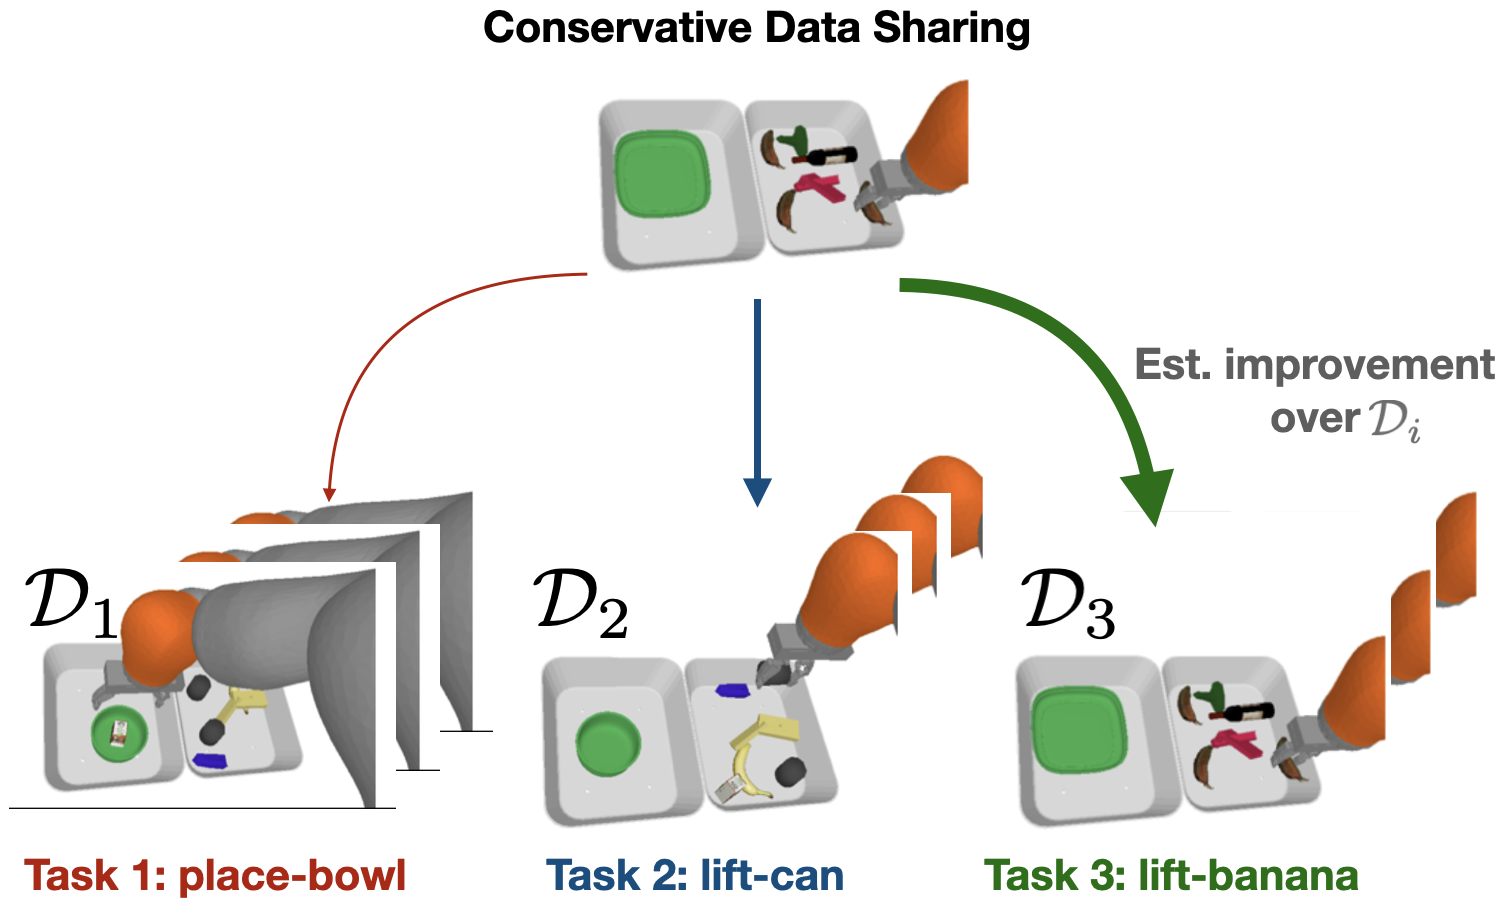
\includegraphics[width=0.45\textwidth]{chapters/cds/cds_teaser.png}
%   %%SL.7.31: consider making this a wrapfigure
%   \vspace{-0.2cm}
%   \caption{\footnotesize A visualization of \cdsmethodname, which routes a transition to
%   the offline dataset $\mathcal{D}_i$ for each task $i$ with a weight based on the estimated improvement over the behavior policy $\pi_\beta(\ba|\bs, i)$ of $\mathcal{D}_i$ after sharing the transition.}
%   \label{fig:teaser}
%   \vspace{-0.3cm}
% \end{wrapfigure}


\subsection{When Does Data Sharing Actually Help in Offline Multi-Task RL?}
\label{sec:analysis}
\vspace{-0.1cm}

Our goal is to leverage experience from all tasks to learn a policy for a particular task of interest. Perhaps the simplest approach to leveraging experience across tasks is to train the task policy on not just the data coming from that task, but also relabeled data from all other tasks~\citep{caruana1997multitask}. Is this na\"ive data sharing strategy sufficient for learning effective behaviors from multi-task offline data? In this section, we aim to answer this question via empirical analysis on a relatively simple domain, which will reveal interesting aspects of data sharing. We first describe the experimental setup and then discuss the results and possible explanations for the observed behavior. Using insights obtained from this analysis, we will then derive a simple and effective data sharing strategy in Section~\ref{sec:method}.

\textbf{Experimental analysis setup.} To assess the efficacy of data sharing, we experimentally analyze various multi-task RL scenarios created with the walker2d environment in Gym~\citep{brockman2016openai}. We construct different test scenarios on this environment that mimic practical situations, including settings where different amounts of  data of varied quality are available for different tasks~\citep{kalashnikov2021mt,xie2019improvisation,singh2020parrot}. In all these scenarios, the agent attempts three tasks: \texttt{run forward}, \texttt{run backward}, and \texttt{jump}, which we visualize in Figure~\ref{fig:env}. Following the problem statement in Section~\ref{sec:prelims}, these tasks share the same state-action space and transition dynamics, differing only in the reward function that the agent is trying to optimize. 
Different scenarios are generated with varying size offline datasets, each collected with policies that have different degrees of suboptimality. This might include, for each task, a single policy with mediocre or expert performance, or a mixture of policies given by the initial part of the replay buffer trained with online SAC~\citep{haarnoja2018soft}. We refer to these three types of offline datasets as medium, expert and medium-replay, respectively, following \citet{fu2020d4rl}.

We train a single-task policy $\pi_\mathrm{CQL}(\mathbf{a}|\bs, i)$ with CQL~\citep{kumar2020conservative} as the base offline RL method, along with two forms of data-sharing, as shown in Table~\ref{tab:analysis}: no sharing of data across tasks (\textbf{No Sharing}) and complete sharing of data with relabeling across all tasks (\textbf{Sharing All}). In addition, we also measure the divergence term in Equation~\ref{eqn:generic_multitask_offline_rl}, $D(\pi(\cdot|\cdot, i), \pi^\mathrm{eff}_\beta(\cdot|\cdot, i))$, for $\pi = \pi_\mathrm{CQL}(\mathbf{a}|\bs, i)$, averaged across tasks by using the
Kullback-Liebler divergence. This value quantifies the average divergence between the single-task optimal policy and the relabeled behavior policy averaged across tasks.  

\begin{table*}[t]
\centering
\scriptsize
\def\arraystretch{0.9}
\setlength{\tabcolsep}{0.42em}
\resizebox{0.95\textwidth}{!}{\begin{tabular}{cc|cc|cc}
  \toprule
 \multicolumn{1}{c}{\multirow{1.5}[2]{*}{Dataset types / Tasks}} & \multicolumn{1}{c}{\multirow{1.5}[2]{*}{Dataset Size}}\vline &
 \multicolumn{2}{c}{Avg Return}\vline & \multicolumn{2}{c}{$D_\text{KL}(\pi, \pi_\beta)$}\\
 & \multicolumn{1}{c}{}\vline & \multicolumn{1}{c}{\textbf{No Sharing}}  & \multicolumn{1}{c}{\textbf{Sharing All}}\vline  & \multicolumn{1}{c}{\textbf{No Sharing}}  & \multicolumn{1}{c}{\textbf{Sharing All}} \\
\midrule
  medium-replay / \texttt{run forward} & 109900 & \textbf{998.9} & 966.2 & \textbf{3.70} & 10.39\\
  medium-replay / \texttt{run backward} & 109980 & \textbf{1298.6} & 1147.5 & \textbf{4.55} & 12.70\\
  medium-replay / \texttt{jump} & 109511 & \textbf{1603.1} & 1224.7 & \textbf{3.57} & 15.89\\
  \rowcolor{Gray}
  \textbf{average task performance} & N/A & \textbf{1300.2} & 1112.8 & \textbf{3.94}  & 12.99\\
  \midrule
  medium / \texttt{run forward} & 27646 & 297.4  & \textbf{848.7} &\textbf{6.53} & 11.78\\
  medium / \texttt{run backward} & 31298 & 207.5 & \textbf{600.4}& \textbf{4.44} & 10.13\\
  medium / \texttt{jump} & 100000 & 351.1 & \textbf{776.1}& \textbf{5.57} & 21.27\\
%   \hline
\rowcolor{Gray}
  \textbf{average task performance} & N/A & 285.3 & \textbf{747.7} & \textbf{5.51} & 14.39 \\
  \midrule
  medium-replay / \texttt{run forward} & 109900 & 590.1 & \textbf{701.4}& \textbf{1.49} & 7.76\\
  medium / \texttt{run backward} & 31298 & 614.7 & \textbf{756.7}& \textbf{1.91} & 12.2\\
  \rowcolor{yellow}
  expert / \texttt{jump} & 5000 & \textbf{1575.2} & 885.1 & \textbf{3.12} & 27.5\\
%   \hline
\rowcolor{Gray}
  \textbf{average task performance} & N/A & \textbf{926.6} & 781 & \textbf{2.17}  & 15.82 \\
    \bottomrule
\end{tabular}}
    \vspace{-0.1cm}
         \caption{\footnotesize We analyze how sharing data across all tasks (\textbf{Sharing All}) compares to \textbf{No Sharing} in the multi-task walker2d environment with three tasks: run forward, run backward, and jump. We provide three scenarios with different styles of per-task offline datasets in the leftmost column. The second column shows the number of transitions in each dataset. We report the per-task average return, the KL divergence between the single-task optimal policy $\pi$ and the behavior policy $\behavior$ after the data sharing scheme, as well as averages across tasks. \textbf{Sharing All} generally helps training while increasing the KL divergence. However, on the row highlighted in yellow, \textbf{Sharing All} yields a particularly large KL divergence between the single-task $\pi$ and $\behavior$ and degrades the performance, suggesting sharing data for all tasks is brittle.
     \label{tab:analysis}
     \vspace{-0.2cm}
     }
\end{table*}

\textbf{Analysis of results in Table~\ref{tab:analysis}.} To begin, note that even na\"ively sharing data is  better than not sharing any data at all on \textbf{5/9} tasks considered
(compare the performance across \textbf{No Sharing} and \textbf{Sharing All} in Table~\ref{tab:analysis}). However, a closer look at Table~\ref{tab:analysis} suggests that data-sharing can significantly degrade performance on certain tasks, especially in scenarios where the amount of data available for the original task is limited, and where the distribution of this data is narrow.
For example, when using expert data for jumping in conjunction with more than 25 times as much lower-quality (mediocre \& random) data for running forward and backward, we find that the agent performs poorly on the jumping task despite access to near-optimal jumping data.

~

\niparagraph{\emph{Why does na\"ive data sharing degrade performance on certain tasks despite near-optimal behavior for these tasks in the original task dataset?}} We argue that the primary reason that na\"{i}ve data sharing can actually hurt performance in such cases is because it exacerbates the distributional shift issues that afflict offline RL. Many offline RL methods combat distribution shift by implicitly or explicitly constraining the learned policy to stay close to the training data. Then, when the training data is changed by adding relabeled data from another task, the constraint causes the learned policy to change as well. When the added data is of low quality for that task, it will correspondingly lead to a lower quality learned policy for that task, unless the constraint is somehow modified. This effect is evident from the higher divergence values between the learned policy without any data-sharing and the effective behavior policy for that task \emph{after} relabeling (e.g., expert+\texttt{jump}) in Table~\ref{tab:analysis}. Although these results are only for CQL, we expect that any offline RL method would, insofar as it combats distributional shift by staying close to the data, would exhibit a similar problem. 


\niparagraph{\textbf{To mathematically quantify}} the effects of data-sharing in multi-task offline RL, we appeal to safe policy improvement bounds~\citep{laroche2019safe,kumar2020conservative,yu2021combo} and discuss cases where data-sharing between tasks $i$ and $j$ can degrade the amount of worst-case guaranteed improvement over the behavior policy. Prior work~\citep{kumar2020conservative} has shown that the generic offline RL algorithm in Equation~\ref{eqn:generic_offline_rl} enjoys the following guarantees of policy improvement on the actual MDP, beyond the behavior policy: 
\begin{align}
\label{eqn:spi}
    J(\pi^*) &\geq J(\pi_\beta) - \mathcal{O}(1/ (1 - \gamma)^2) \mathbb{E}_{\bs, \mathbf{a} \sim d^{\pi}} \left[\sqrt{\frac{D(\pi(\cdot|\bs), \pi_\beta(\cdot|\bs))}{|\mathcal{D}(\bs)|}}\right] + \alpha/(1 - \gamma) D(\pi, \pi_\beta).
\end{align}
We will use Equation~\ref{eqn:spi} to understand the scenarios where data sharing can hurt. When data sharing modifies $\mathcal{D} = \mathcal{D}_i$ to $\mathcal{D} = \mathcal{D}^\mathrm{eff}_i$, which includes $\mathcal{D}_i$ as a subset, it effectively aims at reducing the magnitude of the second term (i.e., sampling error) by increasing the denominator. This can be highly effective if the state distribution of the learned policy $\pi^*$ and the dataset $\mathcal{D}$ overlap. However, an increase in the divergence $D(\pi(\cdot|\bs), \pi^\beta(\cdot|\bs))$ as a consequence of relabeling implies a potential increase in the sampling error, unless the increased value of $|\mathcal{D}^\mathrm{eff}(\bs)|$ compensates for this. Additionally, the bound also depends on the quality of the behavior data added after relabeling: if the resulting behavior policy $\pi^\mathrm{eff}_\beta$ is more suboptimal compared to $\pi_\beta$, i.e., $J(\pi^\mathrm{eff}_\beta) < J(\pi_\beta)$, then the guaranteed amount of improvement also reduces.

% \begin{proposition}[Na\"ive data-sharing can hurt policy performance.] Assume that the the multi-task MDP consists of discrete states $\mathcal{S}$ and actions $\mathcal{A}$. Consider the scenario where data from task $\mathcal{T}_j$, $\mathcal{D}(\mathcal{T}_j)$, is relabelled to task $\mathcal{T}_i$ and let $\mathcal{D}_\mathrm{eff}(\mathcal{T}_i) = \mathcal{D}(\mathcal{T}_j \rightarrow \mathcal{T}_i) \cup \mathcal{D}(\mathcal{T}_i)$. For any dataset, let $|\mathcal{D}(\bs)|$ be the frequency of a state $\bs$ in $\mathcal{D}$, $\pi^*(\mathbf{a}|\bs, \mathcal{T}_i)$ denote the optimal solution to Equation~\ref{eqn:generic_multitask_offline_rl} without any data sharing and let $\pi^*_\mathrm{eff}(\mathbf{a}|\bs)$ be the optimal solution of Equation~\ref{eqn:generic_multitask_offline_rl} with data sharing. Let $\pi^\mathrm{eff}_\beta(\mathbf{a}|\bs, \mathcal{T}_i)$ denote the effective behavior policy for $\mathcal{D}_\mathrm{eff}(\mathcal{T}_i)$. Then, sharing data from task $\mathcal{T}_j$ to task $\mathcal{T}_i$ may not improve the resulting policy performance on task $\mathcal{T}_i$, i.e., $J(\pi^*, \mathcal{T}_i) \geq J(\pi^*_\mathrm{eff}, \mathcal{T}_i) + \zeta$, in the worst-case where:
% \begin{equation*}
%     \zeta \geq  C \mathbb{E}_{\bs, \mathbf{a} \sim d^{\pi^*}} \left[ \sqrt{\frac{D(\pi(\cdot|\bs), \pi^\mathrm{eff}_\beta(\cdot|\bs))}{{|\mathcal{D}_\mathrm{eff}(\mathcal{T}_i)(\bs)|}}} \right] - C \mathbb{E}_{\bs, \mathbf{a} \sim d^{\pi^*}} \left[ \sqrt{\frac{D(\pi(\cdot|\bs), \pi_\beta(\cdot|\bs))}{{|\mathcal{D}(\mathcal{T}_i)(\bs)|}}} \right] + J_{\mathcal{T}_i}(\pi_\beta) - J_{\mathcal{T}_i}(\pi_\beta^\mathrm{eff}) 
% \end{equation*}
% where $C$ is a universal constant depending on the MDP, $d^{\pi^*}$ denotes the state-action marginal of policy $\pi^*$ on the MDP and $\varepsilon > 0$.
% \label{prop:data_sharing}
% \end{proposition}
% While the inequality in Proposition~\ref{prop:data_sharing} is only a bound on performance, it still reveals some tradeoffs associated with data sharing: when data sharing induces distributional shift, such that the value of $D(\pi, \pi^\mathrm{eff}_\beta)$ increases compared to $D(\pi, \pi_\beta)$, without increasing visitation frequencies of states under the learned single-task policy, such that $|\mathcal{D}_\mathrm{eff}(\mathcal{T}_i)(\bs)|$ does not increase enough
% beyond $|\mathcal{D}(\mathcal{T}_i)(\bs)|$ to compensate for the increase in $D(\pi, \pi^\mathrm{eff}_\beta)$, poor performance might be obtained.
% %%SL.5.23: what about the proposition indicates that poor performance might be obtained? can we make this part of the statement more precise?
% The performance decrease is exacerbated when the data being shared is of low quality, i.e., $J(\pi_\beta^\mathrm{eff}) \leq J(\pi_\beta)$. 
% %%AK: maybe we should also have a figure illustrating the spectrum of data-sharing: there is an optimistic end, share everything, a conservative end, share nothing and the more conservative side of the spectrum where our method lies? This is kinda like what I had drawn earlier on the jamboard notes when we discussed a few months back.

% Two considerations: (1) task alignment (2) different dataset types, which can hurt optimziation. Summarioze the main "rules", phenomenon by this this happens. Consequences -- conservative or you become optimistic, etc
% To conclude, we observe that while na\"ive data sharing can generally help improve performance in multi-task offline RL, but that the behavior policy coupled with the amount of data observed can have a significant impact on the performance of na\"ive data sharing. This may prevent existing algorithms from leveraging large pre-existing datasets of potentially useful, but not directly-relevant behaviors to improve performance, thereby hindering generalization. In the next section, we present our method, \cdsmethodname,  that addresses this issue and is derived via a principled optimization problem that aims to maximize per-task performance.

\textbf{To conclude,} our analysis reveals that while data sharing is often helpful in multi-task offline RL, it can lead to substantially poor performance on certain tasks as a result of exacerbated distributional shift between the optimal policy and the effective behavior policy induced after sharing data. 
% Thus, in order to obtain effective policies for all tasks in this setting, we propose to share data \emph{conservatively},
% with precaution taken to not exacerbate distributional shift via relabeling. This forms the basis of our data-sharing scheme, \cdsmethodname, which we will discuss next.

% \vspace{-5pt}
% \section{Regimes of Data Sharing in Multi-Task Offline RL}
% \label{sec:different_regimes}
% The analysis in Section~\ref{sec:analysis} shows that na\"ive data sharing may be highly sub-optimal in some cases, and although it often does improve over no data sharing at all in practice, it can also lead to exceedingly poor performance. On the other hand, no data sharing can also lead to poor performance since it is overly conservative, and does not share any experience at all. In this section, we aim to understand the spectrum in between no data sharing and complete data sharing, aiming to understand the kinds of data sharing schemes that provide a balanced tradeoff between no data sharing and full data sharing. We will then use the insights gathered from this section to derive a complete method in Section~\ref{sec:method}.

% Since full data sharing exacerbates distributional shift, a simple data sharing strategy could be to share data only when distributional shift is reduced. That is, more formally, for any given transition $(\bs, \mathbf{a}, r, \bs')$, this scheme would compare $D(\pi, \pi_\beta)(\bs)$ and $D(\pi, \pi^{\text{eff}}_\beta)(\bs)$ and utilize the transition for training only when $D(\pi, \pi_\beta)(\bs) \geq D(\pi, \pi_\beta^\text{eff})(\bs)$. We refer to this scheme as X. 

% While X provably alleviates the concerns of increasing distribution shift as a result of data sharing, it is overly conservative in practice. A distinct, more optimistic scheme for data sharing is to share a use a transition $(\bs, \mathbf{a}, r, \bs')$ for training only if the resulting data improves upon the learned policy performance.   

\vspace{-5pt}
\subsection{\cdsmethodname: Reducing Distributional Shift in Multi-Task Data Sharing}
\label{sec:method}
\vspace{-5pt}
The analysis in Section~\ref{sec:analysis} shows that na\"ive data sharing may be highly sub-optimal in some cases, and although it often does improve over no data sharing at all in practice, it can also lead to exceedingly poor performance. Can we devise a conservative approach that shares data intelligently to not exacerbate distributional shift as a result of relabeling?
%%CF.8.1: This question above is super long, and starts to get incomprehensible towards the end. Can you shorten or split it up? And, what's the difference between the benefits of sharing data and the benefits of sharing data of high quality?? I think that my suggested edit should fix this.
%%AK: addressed, just kept the first part of this since the story of quality and sampling error comes in after 5.1

\subsubsection{A First Attempt at Designing a Data Sharing Strategy}
A straightforward data sharing strategy is to utilize a transition for training only if it reduces the distributional shift.
%%SL.8.1: The above sentence comes across as a bit obtuse -- of course doing X only if it reduces distributional shift will, by definition, not increase distributional shift -- can you rephrase?
%%CF.8.1: +1. Maybe "A starightforward data sharing strategy is to utilize a transition for training only if it reduces the distribution shift."
%%AK: done
Formally, this means that for a given transition $(\bs, \mathbf{a}, r_j(\bs, \mathbf{a}), \bs') \in \mathcal{D}_j$ sampled from the dataset $\mathcal{D}_j$, such a scheme would prescribe using it for training task $i$ (i.e., $(\bs, \mathbf{a}, r_i(\bs, \mathbf{a}), \bs') \in \mathcal{D}^\mathrm{eff}_i$) only if: 
%%CF.8.1: can you simplify the structure of the above sentence? it is a lot to take in and will probably require the reader to read it twice in its current form.
%%AK: slightly reogranized. Is it still too hard to read?
\begin{tcolorbox}[colback=blue!6!white,colframe=black,boxsep=0pt,top=-3pt,bottom=2pt]
\begin{equation}
\label{eqn:pessimistically_conservative}
    \text{\textbf{CDS (basic)}:}~~~~~~~\Delta^\pi(\bs, \mathbf{a}) := D(\pi(\cdot|\cdot, i), \pi_\beta(\cdot|\cdot, i))(\bs) - D(\pi(\cdot|\cdot, i), \pi_\beta^{\text{eff}}(\cdot|\cdot, i))(\bs) \geq 0. 
\end{equation}
\end{tcolorbox}
%%AK: the above equation is not technically correct, since there is no a on the right side of \Delta^\pi(s, a), need to fix this.
The scheme presented in Equation~\ref{eqn:pessimistically_conservative} would guarantee that distributional shift (i.e., second term in Equation~\ref{eqn:generic_multitask_offline_rl}) is reduced.
%%CF.8.1: i.e. that distribution shift is reduced.
%%AK: done
Moreover, since sharing data can only increase the size of the dataset and not reduce it, this scheme is guaranteed to not increase the sampling error term in Equation~\ref{eqn:spi}. We refer to this scheme as the basic variant of conservative data sharing (\textbf{CDS (basic)}).
%%CF.8.1: hmm, I wouldn't recommend forward referencing equations like this.
%%AK: this was an error in the equatino refercing, this question appears before.

While this scheme can prevent the negative effects of increased distributional shift, this scheme is quite pessimistic. Even in our experiments, we find that this variant of CDS does not improve performance by a large margin.
%%TY.8.2: did our experiments show this? Maybe we should rephrase to "we find that this variant of CDS performs underwhelmingly, achieving worse results compared to the naively data sharing and no data sharing approaches".
%%AK: done
Additionally, as observed in Table~\ref{tab:analysis} (medium-medium-medium data composition) and discussed in Section~\ref{sec:analysis}, data sharing can often be useful despite an increased distributional shift (note the higher values of $D_\mathrm{KL}(\pi, \pi_\beta)$ in Table~\ref{tab:analysis}) likely because it reduces sampling error and potentially utilizes data of higher quality for training. \textbf{CDS (basic)} described above does not take into account these factors. Formally, the effect of the first term in Equation~\ref{eqn:generic_multitask_offline_rl}, $J_{\mathcal{D}^\text{eff}}(\pi)$ (the policy return in the empirical MDP generated by the dataset) and a larger increase in $|\mathcal{D}^\mathrm{eff}(\bs)|$ at the cost of somewhat increased value of $D(\pi(\cdot|\bs), \pi_\beta(\cdot|\bs)$ are not taken into account. Thus we ask: can we instead design a more complete version of CDS that effectively balances the tradeoff by incorporating all the discussed factors (distributional shift, sampling error, data quality)?  
% This term is guaranteed to increase with the scheme in Equation~\ref{eqn:pessimistically_conservative} in practice, since this scheme only utilizes \emph{additional} data corresponding to other tasks for training which would not reduce the performance of the policy compared to no sharing. Combined with the reduced value of the second term, this implies that this scheme increases the objective in Equation~\ref{eqn:generic_multitask_offline_rl}. 

%%SL.8.1: In the interest of space, I think this paragraph can largely be cut, since the end of the previous paragraph already motivates the need for a less conservative method. You could cut this and replace it with a sentence or two at the beginning of the next section.
%%CF.8.1: +1
% \textbf{Is p-CDS sufficient for effective multi-task offline RL?} While p-CDS guarantees that the shared data will not exacerbate distributional shift, which is quite useful in cases such as the walker2d expert scenario analyzed in Section~\ref{sec:analysis}, this scheme can be overly pessimistic. As we also find in our experiments in Section~\ref{sec:exp}, p-CDS often chooses to not share any data in scenarios where it is impossible to meet the strong requirement of reduced distributional shift. On the other side, in a number of scenarios, data sharing improves performance because more training data stabilizes training and reduces sampling error and improves the quality of the data in the dataset, albeit at the cost of slightly increased distributional shift. This raises the question: Can we devise a conservative data sharing scheme that instead \emph{optimistically} shares data, by effectively balancing the improvement due to reduced sampling error and increased data quality, and a deterioration due to increased distributional shift? Such an optimistic scheme would not only reduce the second term in Equation~\ref{eqn:generic_multitask_offline_rl}, but would also share data if the gain in the first term $J_{\mathcal{D}^\text{eff}}(\pi)$ outweighs a slight increase in distributional shift. This is the key idea behind \textbf{optimistically conservative data sharing (o-CDS)} that we discuss next.

\subsubsection{The Complete Version of Conservative Data Sharing (CDS)}
\label{sec:complete_cds}
\begin{wrapfigure}{r}{0.5\textwidth}
\centering
\vspace{-0.7cm}
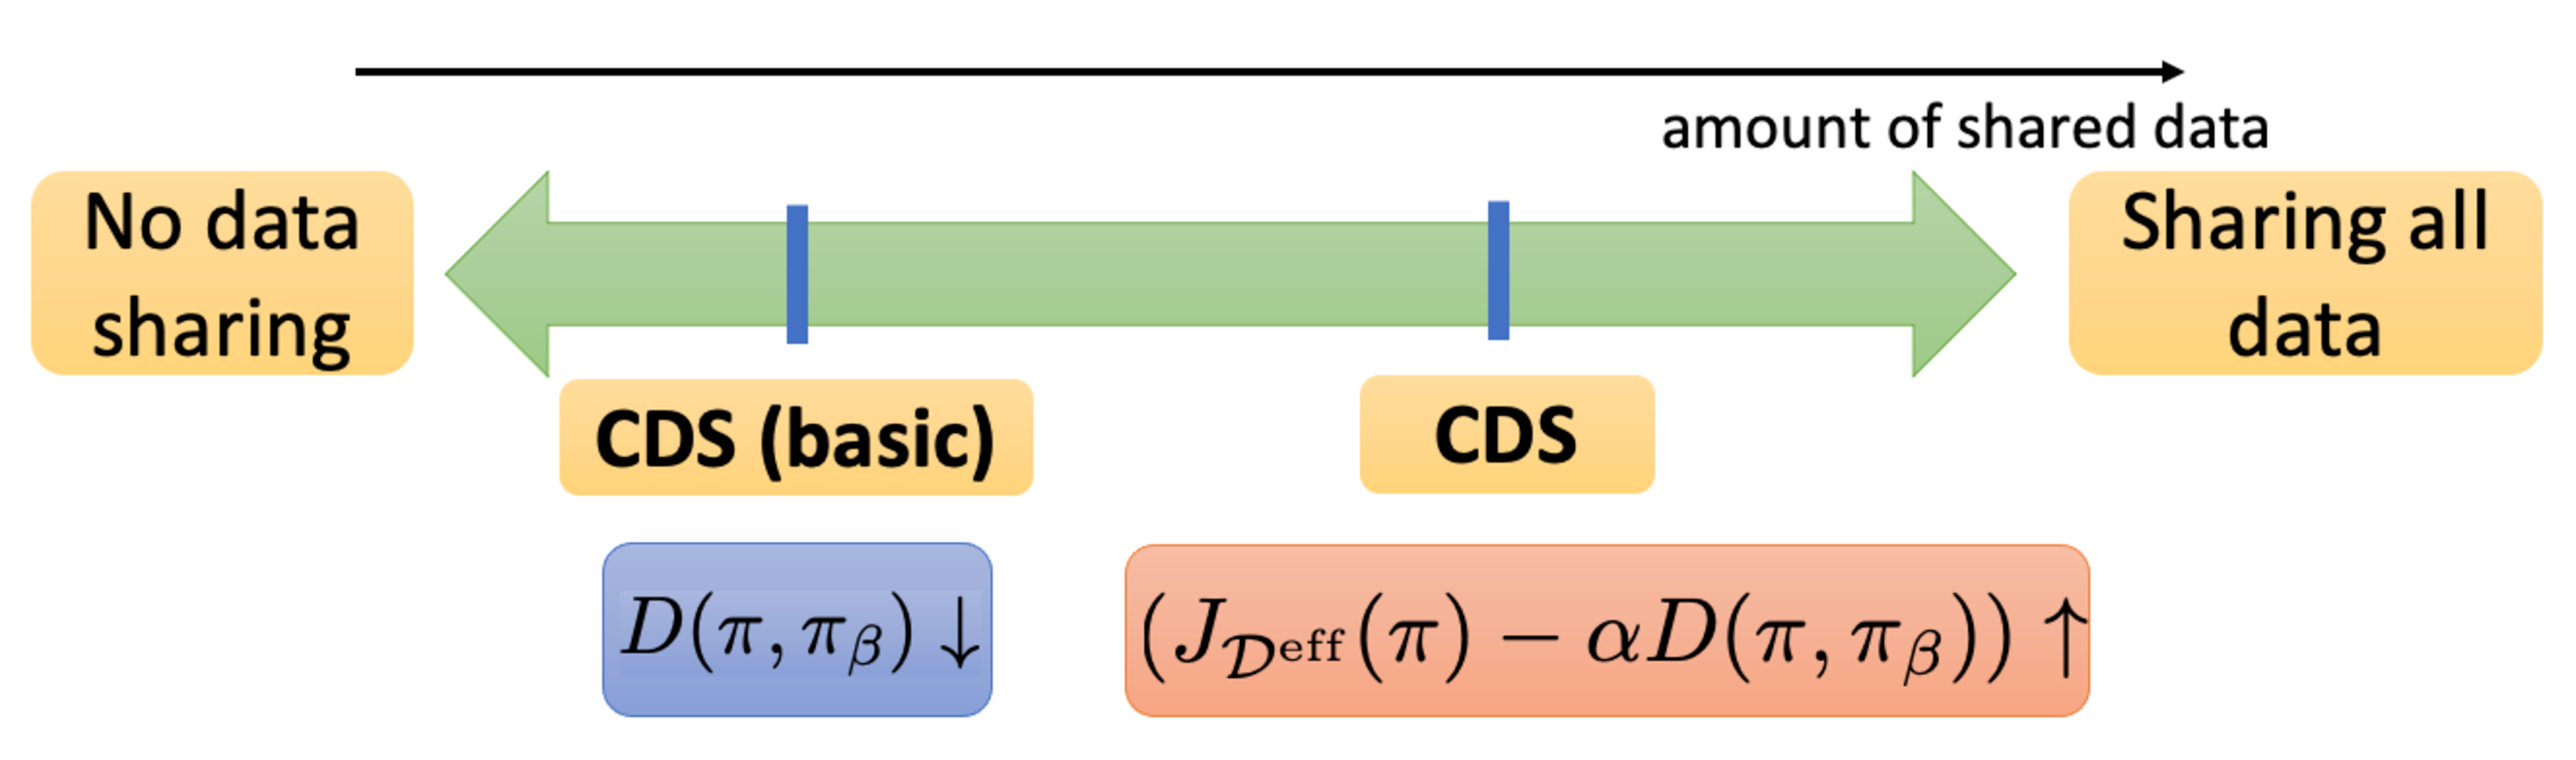
\includegraphics[width=0.99\linewidth]{chapters/cds/cds_variants.pdf}
%%CF.8.1: I think this is a nice figure. My only comment is that it isn't clear what "naive data sharing" means without having read parts of the main text. (and you should expect readers to skim figures without reading all of the text. I would change it to something like "Sharing all data" instead.
\vspace{-0.6cm}
\caption{\label{fig:cds_variants_main} \footnotesize A schematic comparing \textbf{CDS} and \textbf{CDS (basic)} data sharing schemes relative to no sharing (left extreme) and full data sharing (right extreme). While p-CDS only shares data when distributional shift is strictly reduced, o-CDS is more optimistic and shares data when the objective in Equation~\ref{eqn:generic_multitask_offline_rl} is larger. Typically, we would expect that CDS shares more transitions than CDS (basic).}
\vspace{-0.6cm}
\end{wrapfigure}
Next, we present the complete version of our method. The complete version of CDS, which we will refer to as \textbf{CDS}, for notational brevity is derived from the following perspective: we note that a data sharing scheme can be viewed as altering the dataset $\mathcal{D}^\mathrm{eff}_i$, and hence the effective behavior policy, $\pi^\mathrm{eff}_\beta(\mathbf{a}|\bs, i)$.
Thus, we can directly \emph{optimize} the objective in Equation~\ref{eqn:generic_multitask_offline_rl} with respect to $\pi^\mathrm{eff}_\beta$,
in addition to $\pi$, where $\pi^\mathrm{eff}_\beta$ belongs to the set of all possible effective behavior policies that can be obtained via any form of data sharing. Note that unlike CDS (basic), this approach would not rely on only indirectly controlling the objective in Equation~\ref{eqn:generic_multitask_offline_rl} by controlling distributional shift, but would aim to directly optimize the objective in Equation~\ref{eqn:generic_multitask_offline_rl}.  We formalize this optimization below in Equation~\ref{eqn:optimize_behavior}:
\begin{align}
\label{eqn:optimize_behavior}
    % &(\pi^*(\cdot|\cdot, i), \pi^\mathrm{eff}_\beta(\cdot|\cdot, i))\nonumber\\
    \arg \max_{\pi} \textcolor{red}{\max_{\pi^\mathrm{eff}_\beta \in \Pi_{\mathrm{relabel}}}}~~~ \left[J_{\mathcal{D}^\mathrm{eff}_i}(\pi) - \alpha D(\pi, \pi^\mathrm{eff}_\beta; i)\right],
\end{align}
where $\Pi_{\mathrm{relabel}}$ denotes the set of all possible behavior policies that can be obtained via relabeling. The next result characterizes safe policy improvement for Equation~\ref{eqn:optimize_behavior} and discusses how it leads to improvement over the behavior policy and also produces an effective practical method.

\begin{tcolorbox}[colback=blue!6!white,colframe=black,boxsep=0pt,top=-3pt,bottom=2pt]
\vspace{2mm}
\begin{proposition}[Characterizing safe-policy improvement for CDS.] 
\label{prop:spi_thm}
Let $\pi^*(\mathbf{a}|\bs)$ be the policy obtained from Equation~\ref{eqn:optimize_behavior}, and let $\pi_\beta(\mathbf{a}|\bs)$ be the behavior policy for $\mathcal{D}_i$. Then, w.h.p. $\geq 1 - \delta$, $\pi^*$ is a $\zeta$-safe policy improvement over $\pi_\beta$, i.e., $J(\pi^*) \geq J(\pi_\beta) - \zeta$, where $\zeta$ is given by:
\begin{align*}
\small{
    \!\!\zeta = \mathcal{O}\left(\frac{1}{(1 - \gamma)^2}\right)  \mathbb{E}_{\bs \sim d^{\pi^*}_{\mathcal{D}^\mathrm{eff}_i}}\left[\sqrt{\frac{D_{\text{CQL}}(\pi^*, \pi_\beta^*)(\bs) + 1}{|\mathcal{D}^\mathrm{eff}_i(\bs)|}} \right]
    -  \left[\alpha D(\pi^*, \pi_\beta^*) + \underbrace{J(\pi^*_\beta) - J(\pi_\beta)}_{\text{(a)}} \right],}
\end{align*}
\!\!where $\mathcal{D}^\mathrm{eff}_i \sim d^{\pi_\beta^*}(\bs)$ and $\pi^*_\beta(\mathbf{a}|\bs)$ denotes the policy $\pi \in \Pi_{\text{relabel}}$ that maximizes Equation~\ref{eqn:optimize_behavior}. 
\end{proposition}
\end{tcolorbox}
%%CF.8.1: I might consider putting this theoretical result back to the appendix. Right now, the main method doesn't come until the bottom of page 7, and the practical implementation doesn't come until page 8. Given that you can only really expect the reader to read ~9 pages, I think that the core info about the method is more important than this theoretical result.

A proof and analysis of this proposition is provided in Appendix~\ref{app:proofs}, where we note that the bound in Proposition~\ref{prop:spi_thm} is stronger than both no data sharing as well as na\"ive data sharing. We show in Appendix~\ref{app:proofs} that optimizing Equation~\ref{eqn:optimize_behavior} reduces the numerator $D_\mathrm{CQL}(\pi^*, \pi_\beta^*)$ term while also increasing $|\mathcal{D}^\mathrm{eff}_i(\bs)|$, thus reducing the amount of sampling error. In addition, Lemma~\ref{lemma:a_gt_0} shows that the improvement term $(a)$ is guaranteed to be positive if a large enough $\alpha$ is chosen in Equation~\ref{eqn:optimize_behavior}. Combining these, we find data sharing using Equation~\ref{eqn:optimize_behavior} improves over both complete data sharing (which may increase $D_\mathrm{CQL}(\pi, \pi_\beta)$) and no data sharing (which does not increase $|\mathcal{D}^\mathrm{eff}_i(\bs)|$). A schematic comparing the two variants of CDS and na\"ive and no data sharing schemes is shown in Figure~\ref{fig:cds_variants_main}.

~

\niparagraph{\textbf{Optimizing Equation~\ref{eqn:optimize_behavior} tractably.}} 
The next step is to effectively convert Equation~\ref{eqn:optimize_behavior} into a simple condition for data sharing in  multi-task offline RL. While directly solving Equation~\ref{eqn:optimize_behavior} is intractable in practice, since both the terms depend on $\pi^\mathrm{eff}_\beta(\mathbf{a}|\bs)$ (since the first term $J_{\mathcal{D}^\mathrm{eff}}(\pi)$ depends on the empirical MDP induced by the effective behavior policy and the amount of sampling error), we need to instead  solve Equation~\ref{eqn:optimize_behavior} approximately. Fortunately, we can optimize a \textit{lower-bound approximation} to Equation~\ref{eqn:optimize_behavior} that uses the dataset state distribution for the policy update in Equation~\ref{eqn:optimize_behavior} similar to modern actor-critic methods~\citep{degris2012off,lillicrap2015continuous,fujimoto2018addressing,haarnoja2018soft,kumar2020conservative} which only introduces an additional $D(\pi, \pi_\beta)$ term in the objective. This objective is given by: $\mathbb{E}_{\bs \sim \mathcal{D}^{\mathrm{eff}}_i}[\mathbb{E}_\pi[Q(\bs, \mathbf{a}, i)] - \alpha' D(\pi(\cdot|\bs,i), \pi_\beta^\mathrm{eff}(\cdot|\bs,i))]$, which is equal to the expected ``conservative Q-value'' $\hat{Q}^\pi(\bs, \mathbf{a}, i)$ on dataset states, policy actions and task $i$. Optimizing this objective via a co-ordinate descent on $\pi$ and $\pi^\mathrm{eff}_\beta$ dictates that $\pi$ be updated using a standard update of maximizing the conservative Q-function, $\hat{Q}^\pi$ (equal to the difference of the Q-function and $D(\pi, \pi^{\mathrm{eff}}_\beta; i)$).
Moreover, $\pi^{\mathrm{eff}}_\beta$ should also be updated towards maximizing the same expectation, $\mathbb{E}_{\bs, \mathbf{a} \sim \mathcal{D}^\mathrm{eff}_i}[\hat{Q}^\pi(\bs, \mathbf{a}, i)] := \mathbb{E}_{\bs, \mathbf{a} \sim \mathcal{D}^\mathrm{eff}_i}[Q(\bs, \mathbf{a}, i)] - \alpha D(\pi, \pi_\beta^\mathrm{eff}; i)$. This implies that when updating the behavior policy, we should prefer state-action pairs that maximize the conservative Q-function.
% Additionally $\pi^{\mathrm{eff}}_\beta$ should be updated towards minimizing the distribution shift $\mathbb{E}_{\bs, \mathbf{a} \sim \mathcal{D}^\mathrm{eff}_i}[ D(\pi, \pi_\beta^\mathrm{eff}; i)]$, i.e. learning a new behavior policy of task $i$ with minimal distribution shift after relabeling. In the case where $D(\pi, \pi_\beta^\mathrm{eff}; i) = D_\text{CQL}(\pi, \pi_\beta^\mathrm{eff}; i)$, we have the following objective for updating $\pi_\beta$: $\min_{\pi_\beta}\mathbb{E}_{\bs, \mathbf{a} \sim \mathcal{D}^\mathrm{eff}_i}[\hat{Q}^\pi(\bs,\mathbf{a}, i)]$
% \begin{align}
%     J_{\mathcal{D}^\mathrm{eff}_i}(\pi) - \alpha D(\pi, \pi^\mathrm{eff}_\beta; i) &:= \mathbb{E}_{\bs, \mathbf{a} \sim d^\pi_{\mathrm{eff}}}\left[Q(\bs, \mathbf{a}) - \alpha D(\pi, \pi_\right] 
% \end{align}

~

\niparagraph{\textbf{{Deriving the data sharing strategy for CDS.}}}
%%SL.8.1: not clear what the word "condition" means
%%CF.8.1: +1. What condition are you deriving?
%%AK: fixed
Utilizing the insights for optimizing Equation~\ref{eqn:optimize_behavior} tractably, we now present the effective data sharing rule prescribed by CDS. For any given task $i$, we want relabeling to incorporate transitions with the highest conservative Q-value into the resulting dataset $\mathcal{D}^\mathrm{eff}_i$, as this will directly optimize the tractable lower bound on Equation~\ref{eqn:optimize_behavior}. While directly optimizing Equation~\ref{eqn:optimize_behavior} will enjoy benefits of reduced sampling error since $J_{\mathcal{D}^\mathrm{eff}_i}(\pi)$ also depends on sampling error, our tractable lower bound approximation does not enjoy this benefit. This is because optimizing the lower-bound only increases the frequency of a state in the dataset, $|\mathcal{D}^\mathrm{eff}_i(\bs)|$ by atmost 1. To encourage further reduction in sampling error, we modify CDS to instead share all transitions with a conservative Q-value more than the top $k^\text{th}$ quantile of the original dataset $\mathcal{D}_i$, where $k$ is a hyperparameter. This provably increases the objective value in Equation~\ref{eqn:optimize_behavior} still ensuring that term $(a) > 0$ in Proposition~\ref{prop:spi_thm}, while also reducing $|\mathcal{D}^{\mathrm{eff}}_i(\bs)|$ in the denominator. Thus, for a given transition $(\bs, \mathbf{a}, \bs') \in \mathcal{D}_j$,  
\begin{tcolorbox}[colback=blue!6!white,colframe=black,boxsep=0pt,top=-5pt,bottom=5pt]
\begin{align}
   \text{\textbf{CDS}:~~~~~~~~} \!\!\!\!\!\!\!\!\!(\bs, \mathbf{a}, r_i, \bs') \in \mathcal{D}^{\mathrm{eff}}_i  \text{~if~} {\Delta}^\pi(\bs, \mathbf{a})\! := \hat{Q}^\pi(\bs, \mathbf{a}, i) - P_{k\%}\!\left\{\!\hat{Q}^\pi(\bs', \mathbf{a}', i)\!\!: \bs', \mathbf{a}' \sim \mathcal{D}_i\!\right\} \geq 0,
\label{eqn:method}
\end{align}
\end{tcolorbox}
where $\hat{Q}^\pi$ denotes the learned conservative Q-function estimate. If the condition in Equation~\ref{eqn:method} holds for the given $(\bs, \mathbf{a})$, then the corresponding relabeled transition, $(\bs, \mathbf{a}, r_{i}(\bs, \mathbf{a}), \bs')$ is added to $\mathcal{D}^\mathrm{eff}_i$. 

We summarize the pesudocode of CDS in Algorithm~\ref{alg:cds} in Appendix~\ref{app:alg} and include the practical implementation details of CDS in Appendix~\ref{app:details}.

% Our main data-sharing scheme, o-\cdsmethodname, is based on the insight discussed above. o-\cdsmethodname\ first runs any standard conservative offline RL algorithm on each task individually without any data sharing. Consistent with our insight from above, relabeling a transition that contributes a lower conservative Q-value to the current task will only decrease the average conservative Q-value of the effective resulting dataset for this task, whereas the $\pi^\mathrm{eff}_\beta$ is to be optimized to maximize this value. On the other hand, more samples in $\mathcal{D}^\mathrm{eff}_i$ will reduce sampling error. Hence, we employ a simple rule to decide which transitions from the data for other tasks will be relabeled to the current task, say task $i$: o-\cdsmethodname\ checks if the conservative Q-value estimate for this transition under task $i$ is greater than a specific percentile of the conservative Q-value for the original dataset for task $i$, $\mathcal{D}_i$. This is sufficient to increase the average conservative Q-value in $\mathcal{D}^\mathrm{eff}_i$ after relabeling, while still allowing us to keep sampling error under control.

% Thus, o-\cdsmethodname\ first estimates a conservative Q-value estimate, $\hat{Q}^\pi(\bs, \mathbf{a}, i)$ (which can be obtained via any offline RL algorithm), and for a given transition, $(\bs, \mathbf{a}, r_j, \bs') \in \mathcal{D}_j$ it then checks if the following condition is satisfied: 

% If the condition in Equation~\ref{eqn:method} holds for the given $(\bs, \mathbf{a})$, then the corresponding relabeled transition, $(\bs, \mathbf{a}, r_{i}(\bs, \mathbf{a}), \bs')$ is added to $\mathcal{D}^\mathrm{eff}_i$. \arxiv{In practice, instead of computing $\mathbb{E}_{\bs', \mathbf{a}' \sim \mathcal{D}_i}\left[ \hat{Q}^\pi(\bs', \mathbf{a}', i) \right]$, we use the $90$-th percentile of $\hat{Q}^\pi(\bs', \mathbf{a}', i)$ $\forall \bs', \mathbf{a}' \in \mathcal{D}_i$.} This rule for relabeling is applied independently on each transition $(\bs, \mathbf{a}, r, \bs') \in \mathcal{D}$. 

% \subsection{{Practical implementation of \cdsmethodname}} 
%%CF.8.1: In the section header and throughout the section, I would just have this discuss the main variant, not both. 
% The pseudocode of CDS is summarized in Algorithm~\ref{alg:cds} in Appendix~\ref{app:alg}. The complete variant of CDS can be directly implemented using the rule in Equation~\ref{eqn:method} with conservative Q-value estimates obtained via any offline RL method that constrains the learned policy to the behavior policy. For implementing \cdsmethodname\ (basic), we reparameterize the divergence $D$ in Equation~\ref{eqn:pessimistically_conservative} to use the learned conservative Q-values. This is especially useful for our implementation since we utilize CQL as the base offline RL method, and hence we do not have access to an explicit divergence. In this case, $\Delta^\pi(\bs, \mathbf{a})$ can be redefined as, $\Delta^\pi(\bs, \mathbf{a}) :=$
% \begin{align}
%     \mathbb{E}_{\bs' \sim \mathcal{D}^i}\left[\mathbb{E}_{\mathbf{a}' \sim \pi}[\hat{Q}(\bs', \mathbf{a}', i)] - \mathbb{E}_{\mathbf{a}'' \sim \mathcal{D}_i}[\hat{Q}(\bs', \mathbf{a}'', i)]\right] - \left(\mathbb{E}_{\mathbf{a}' \sim \pi}[\hat{Q}(\bs, \mathbf{a}', i)] - Q(\bs, \mathbf{a}, i)\right),
% \label{eqn:p-cds}
% \end{align}
% % \begin{align}
% %     \Delta^\pi(\bs, \mathbf{a})  := 
% %     -\left(\mathbb{E}_{\mathbf{a} \sim \mu(\cdot|\bs)}\!\left[Q(\bs,\mathbf{a}, i)\right]\!-\!\mathbb{E}_{\bs', \mathbf{a}' \sim \mathcal{D}_i}\!\left[Q(\bs',\mathbf{a}', i)\right]\right) +
% %     \left(\mathbb{E}_{\bs\sim \mathcal{D}_i, \mathbf{a} \sim \mu(\cdot|\bs)}\!\left[Q(\bs,\mathbf{a}, i)\right]\!-\!\mathbb{E}_{\bs', \mathbf{a}' \sim \mathcal{D}_i}\!\left[Q(\bs',\mathbf{a}', i)\right]\right)
% % \label{eqn:p-cds}
% % \end{align}
% % where $\mu(\cdot|s)$ is a wide sampling distribution such as the uniform distribution over the range of actions.
% Equation~\ref{eqn:p-cds} can be viewed as the difference between the CQL~\citep{kumar2020conservative} regularization term on a given $(\bs, \mathbf{a})$ and the original dataset for task $i$, $\mathcal{D}_i$. This CQL regularization term is equal to the divergence between the learned policy $\pi(\cdot|\bs)$ and the behavior policy $\pi_\beta(\cdot|\bs)$, therefore Equation~\ref{eqn:p-cds} practically computes Equation~\ref{eqn:pessimistically_conservative}. 
% % Intuitively, if the condition in Equation~\ref{eqn:p-cds} is true for certain $(\bs, \mathbf{a})$, adding it to $\mathcal{D}^\mathrm{eff}_i$ would decrease the expected CQL regularization term, which estimates the distributional shift $D_\text{CQL}(\pi(\cdot|\cdot, i), \pi_\beta^{\text{eff}}(\cdot|\cdot, i))$.

% Finally, both variants of \cdsmethodname\ train a policy, 
% $\pi(\mathbf{a}|\bs; i)$, either conditioned on the task $i$ (i.e., with weight sharing) or a separate $\pi(\mathbf{a}|\bs)$ policy for each task with no weight sharing, using the resulting relabeled dataset, $\mathcal{D}^\mathrm{eff}_i$.
% For practical implementation details of \cdsmethodname\, see Appendix~\ref{app:details}.

%%CF.5.22: you seem to have forgotten the punch line here.

%%SL.5.23: I think it would really help to add some pseudocode that describes the method. Right now, readers have to do a bit of detective work to piece together the complete algorithm. Pseudocode + algorithm summary would really help.

%%AK: just regular CQL weighted by the weights w_(s, a) described above

%%AK: there is a critical point here -- if we keep doing our scheme continually, would we eventually diverge, since we are doing many rounds of relabelling effectively? How should we handle that?



%% Theoretical Analysis

% \subsection{Related Work}
\label{sec:uds_related}

% \textbf{Offline RL.} Offline RL~\citep{ernst2005tree,riedmiller2005neural,LangeGR12,levine2020offline} considers the problem of learning a policy from a static dataset without interacting with the environment, which has shown promises in many practical applications such as robotic control~\citep{kalashnikov2018scalable,Rafailov2020LOMPO}, NLP~\citep{jaques2019way}, 
% and healthcare~\citep{shortreed2011informing, Wang2018SupervisedRL}. 
% The main challenge of offline RL is the distributional shift between the learned policy and the behavior policy~\citep{fujimoto2018off}, which can cause erroneous value backups. To address this issue, prior methods have constrained the learned policy to be close to the behavior policy via policy regularization~\citep{liu2020provably,wu2019behavior,kumar2019stabilizing, zhou2020plas,ghasemipour2021emaq,fujimoto2021minimalist}, conservative value functions~\citep{kumar2020conservative}, 
% and model-based training with conservative penalties~\citep{yu2020mopo,kidambi2020morel,swazinna2020overcoming,lee2021representation,yu2021combo}. Unlike these prior works, we study how unlabeled data can be incorporated into the offline RL framework.

\textbf{RL with unlabeled data.} Prior works tackle the problem of learning from data without reward labels via either directly imitating expert trajectories~\citep{pomerleau1988alvinn,RossB12,GAIL2016Ho}, learning reward functions from expert data using inverse RL~\citep{abbeel2004apprenticeship,ng2000irl,ziebart2008maximum,finn2016guided,AIRLFu2018,konyushkova2020semi}, or learning a reward / value classifier that discriminates successes and failures~\citep{xie2018few,VICEFu2018,singh2019end,eysenbach2021replacing} in standard online RL settings. 
{Unlike these prior works, the goal of our paper is not to propose a sophisticated new algorithm for reward learning,} but rather to study when the simple solution of using zero as the reward label can work well from offline data. {While} \citet{singh2020cog} also considers relabeling prior data with zero reward in the standard, single-task offline RL setting, {the key distinction is that the unlabeled data in \citet{singh2020cog} cannot solve the target task and \emph{actually} gets zero rewards and is thus labeled with the true reward. Unlike \citet{singh2020cog}, we show that UDS can surprisingly also be effective even when the unlabeled data is incorrectly labeled with zero reward, and discuss how it can be improved (Section~\ref{sec:rebalancing}).}
Additionally, we consider both single-task and multi-task offline RL settings.

\textbf{Data sharing.} 
% Sharing data across different tasks has been found to be effective in multi-task~\citep{eysenbach2020rewriting,kalashnikov2021mt,yu2021conservative} and meta-RL~\citep{dorfman2020offline,mitchell2021offline} and it improves performance significantly in multi-task offline RL. 
As discussed in Section~\ref{sec:cds_method}, prior works share data based on learned Q-values~\citep{eysenbach2020rewriting,li2020generalized} (including our CDS approach), domain knowledge~\citep{kalashnikov2021mt}, and other structural quantities such as distance to goals in goal-conditioned settings~\citep{andrychowicz2017hindsight,liu2019competitive,sun2019policy,lin2019reinforcement,chebotar2021actionable}, or the learned distance with robust inference in the offline meta-RL setting~\citep{li2019multi}. However, all of these either require access to the functional form of the reward for relabling or are limited to goal-conditioned settings. In contrast, we attempt to tackle a more general problem where reward labels are not provided for a subset of the data, and find that a simple approach for relabeling data from other tasks with the constant zero (or the minimal possible reward) can work well. 


% \begin{figure}[t]
%     \centering
%     \vspace{-5pt}
%     % 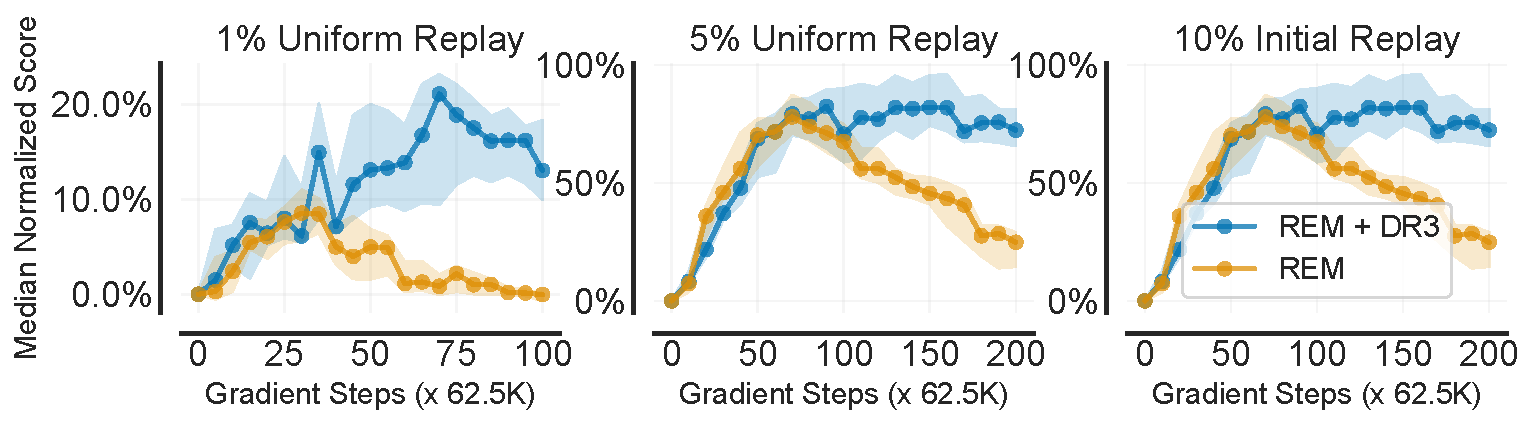
\includegraphics[width=\linewidth]{figures/atari_new/Median_rem_penalty.pdf}
%     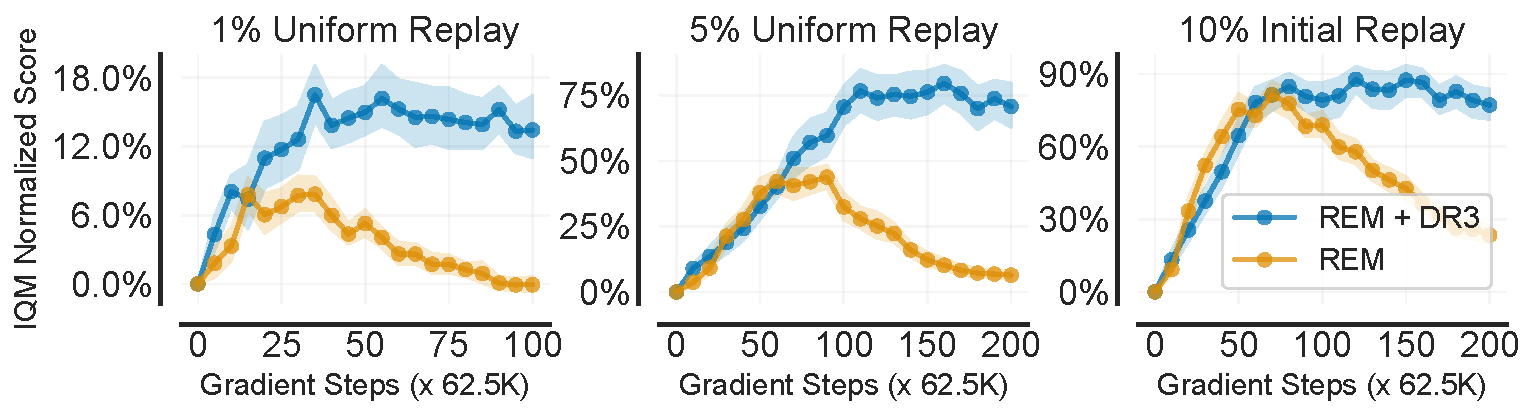
\includegraphics[width=\linewidth]{figures/atari_new/IQM_rem_penalty.pdf}
%     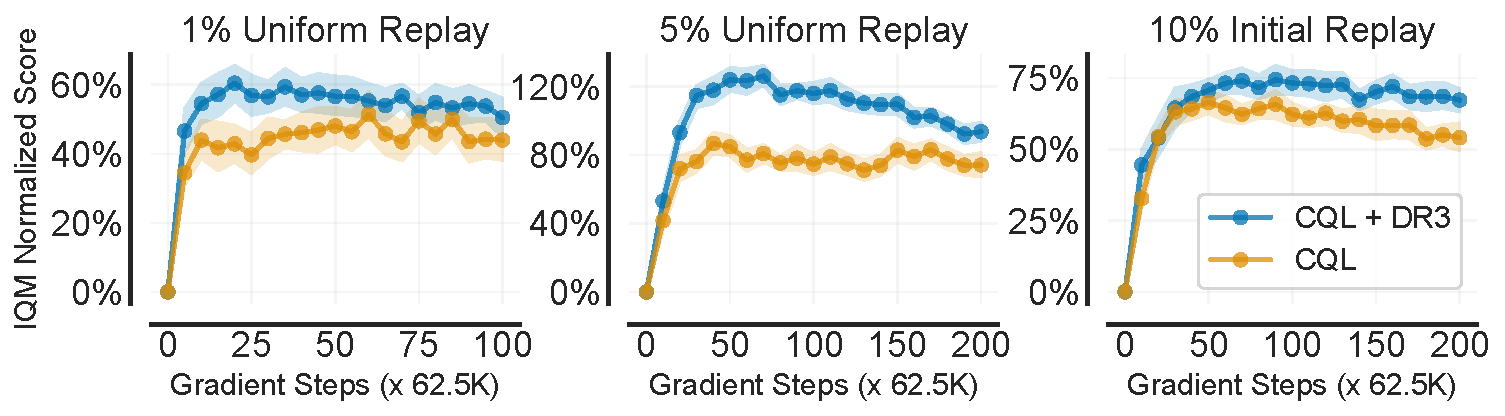
\includegraphics[width=\linewidth]{figures/atari_new/IQM_cql_penalty.pdf}
%     % 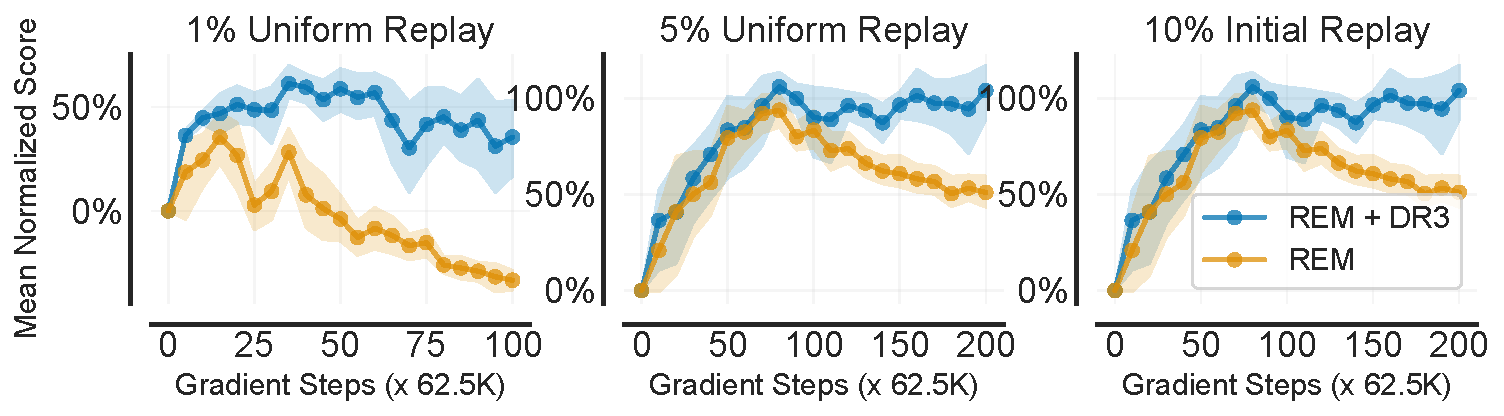
\includegraphics[width=\linewidth]{figures/atari_new/Mean_rem_penalty.pdf}
%     % 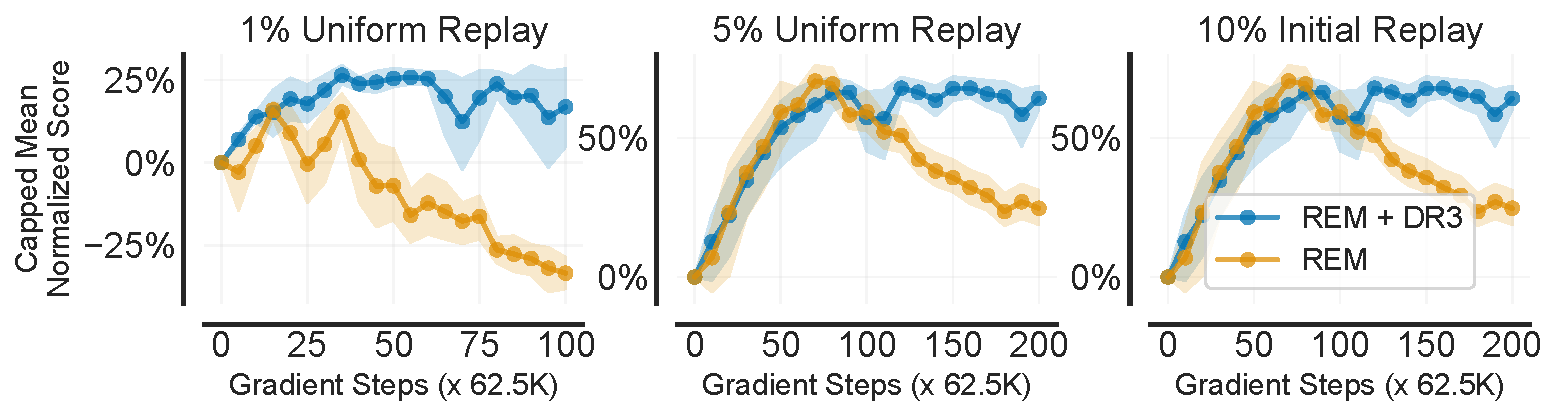
\includegraphics[width=\linewidth]{figures/atari_new/Capped_Mean_rem_penalty.pdf}
%     \vspace{-0.75cm}
%     % \caption{\small{\textbf{Average normalized scores across 17 Atari games for REM + \methodname\ } over the course of training with different dataset types from \citep{agarwal2019optimistic}. Note the increased stability and performance when \methodname\ is used.}}
%     \caption{\small{\textbf{Average normalized scores across 17 Atari games for REM + \methodname\ (top), CQL + \methodname\ (bottom)} over the course of training with different dataset types from prior work~\citep{agarwal2019optimistic}. While na\"ive REM suffers from a degradation in performance with more training, REM + \methodname\ not only remains generally stable with more training, but also attains higher final performance. CQL + \methodname\ attains higher performance.}} %Performance is reported using interquartile mean~(IQM), normalization was performed with respect to the behavior policy that collected the entire DQN replay dataset and shaded regions show 95\% percentile confidence intervals~(CIs.)}}
%     \label{fig:atari_rem_main}
%     \vspace{-0.7cm}
% \end{figure}

\vspace{-0.2cm}
\subsection{Experimental Evaluation}
\label{sec:scaling_exps}
\vspace{-0.2cm}

\begin{figure}[t]
    \centering
    \begin{minipage}{0.65\linewidth}
 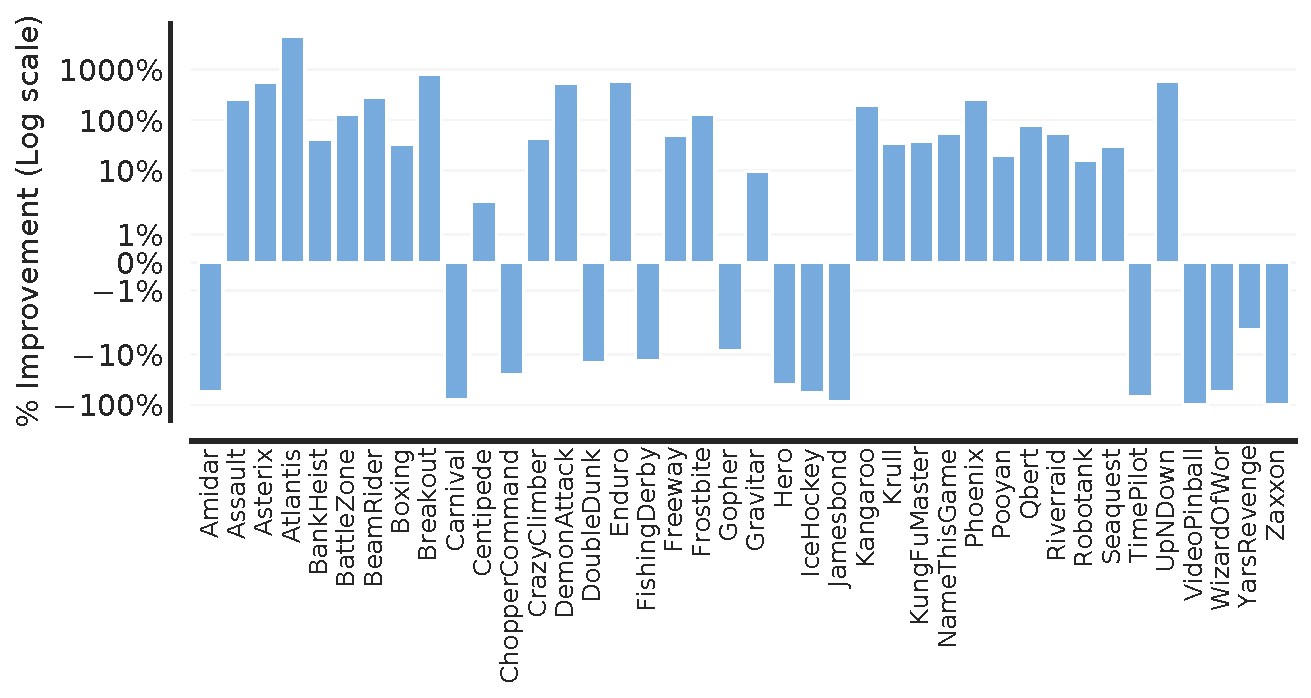
\includegraphics[width=\linewidth]{chapters/scaled_ql/figures/percent_improvement_over_DT.pdf}
    \end{minipage}
    \hfill
    \begin{minipage}{0.34\linewidth}
    \vspace{-0.2cm}
 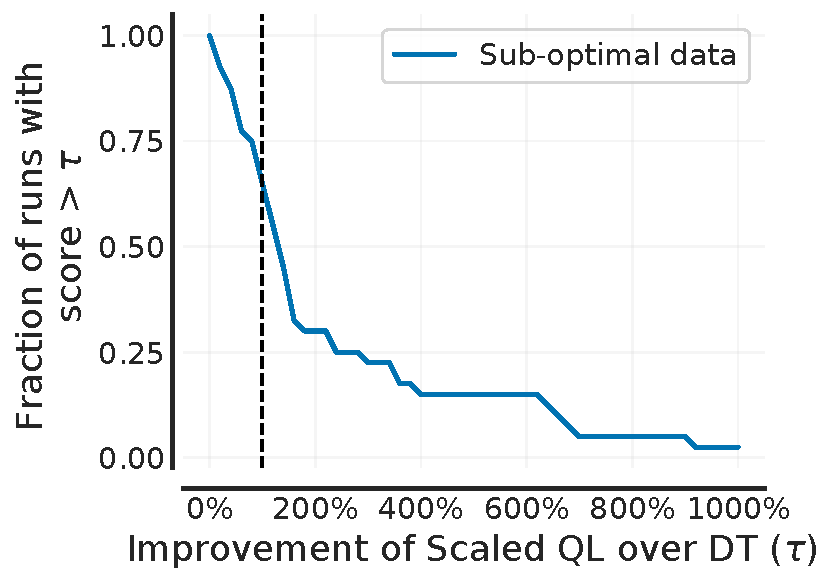
\includegraphics[width=\linewidth]{chapters/scaled_ql/figures/pp_profile_ql_dt.pdf}
    \end{minipage}
    \vspace{-0.4cm}
    \caption{\textbf{Comparing Scaled QL to DT} on all training games on the sub-optimal dataset.}
    \label{fig:percent_improvement}
    \vspace{-0.5cm}
\end{figure}

In our experiments, we study how our approach, scaled Q-learning, can simultaneously learn from sub-optimal and optimal data collected from 40 different Atari games. 
We compare the resulting multi-task policies to behavior cloning~(BC) with same architecture as scaled QL, and the prior state-of-the-art method based on decision transformers (DT)~\citep{chen2021decision}, which utilize return-conditioned supervised learning with large transformers~\citep{lee2022multi}, and have been previously proposed for addressing this task. 
We also study the efficacy of the multi-task initialization produced by scaled Q-learning in facilitating rapid transfer to new games via both offline and online fine-tuning, in comparison to state-of-the-art self-supervised representation learning methods and other prior approaches. Our goal is to answer the following questions: \textbf{(1)} How do our proposed design decisions impact performance scaling with high-capacity models?, \textbf{(2)} Can scaled QL more effectively leverage higher model capacity compared to na\"ive instantiations of Q-learning?, \textbf{(3)} Do the representations learned by scaled QL transfer to new games? We will answer these questions in detail through multiple experiments in the coming sections, but we will first summarize our main results below.


\textbf{Main empirical findings.} Our main results are summarized in Figures~\ref{fig:suboptimal_offline} and \ref{fig:main_results}. These figures show the performance of scaled QL, multi-game decision transformers~\citep{lee2022multi} (marked as ``DT''), a prior method based on supervised learning via return conditioning, and standard behavioral cloning baselines (marked as ``BC'') in the two settings discussed previously, where we must learn from: (i) near optimal data, and (ii) sub-optimal data obtained from the initial 20\% segment of the replay buffer (see our discussion about the problem setup). See Figure~\ref{fig:percent_improvement} for a direct comparison between DT and BC.


\begin{wrapfigure}{r}{0.5\linewidth}
    \vspace{-0.5cm}
    \centering
    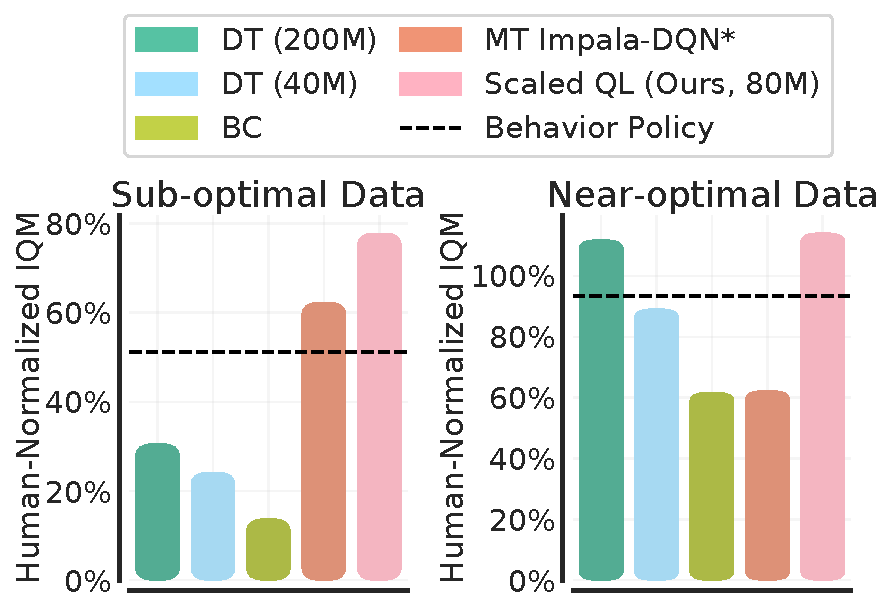
\includegraphics[width=0.95\linewidth]{chapters/scaled_ql/combnined_data_results_iqm.pdf}
    \vspace{-0.25cm}
    \caption{\footnotesize{\textbf{Offline scaled conservative Q-learning vs other prior methods} with near-optimal data and sub-optimal data. Scaled QL outperforms the best DT model, attaining an IQM human-normalized score of \textbf{114.1\%} on the near-optimal data and \textbf{77.8\%} on the sub-optimal data, compared to 111.8\% and 30.6\% for DT, respectively.}}
    \label{fig:main_results}
    \vspace{-0.5cm}
\end{wrapfigure}

In the more challenging sub-optimal data setting, scaled QL attains a performance of \textbf{77.8\%} IQM human-normalized score, although trajectories in the sub-optimal training dataset only attain 51\% IQM human-normalized score. Scaled QL also outperforms the prior DT approach by \textbf{2.5 times} on this dataset, even though the DT model has more than twice as many parameters and uses data augmentation, compared to scaled QL. 

In the $2^{nd}$ setting with near-optimal data, where the training dataset already contains expert trajectories, scaled QL with 80M parameters still outperforms the DT approach with 200M parameters, although the gap in performance is small (3\% in IQM performance, and 20\% on median performance). 
Overall, these results show that scaled QL is an effective approach for learning from large multi-task datasets, for a variety of data compositions including sub-optimal datasets, where we must stitch useful segments of suboptimal trajectories to perform well, and near-optimal datasets, where we should attempt to mimic the best behavior in the offline dataset. 

To the best of our knowledge, these results represent the largest performance improvement over the average performance in the offline dataset on such a challenging problem. We will now present experiments that show that offline Q-learning scales and generalizes.

\begin{figure}[h]
\centering
\vspace{-0.2cm}
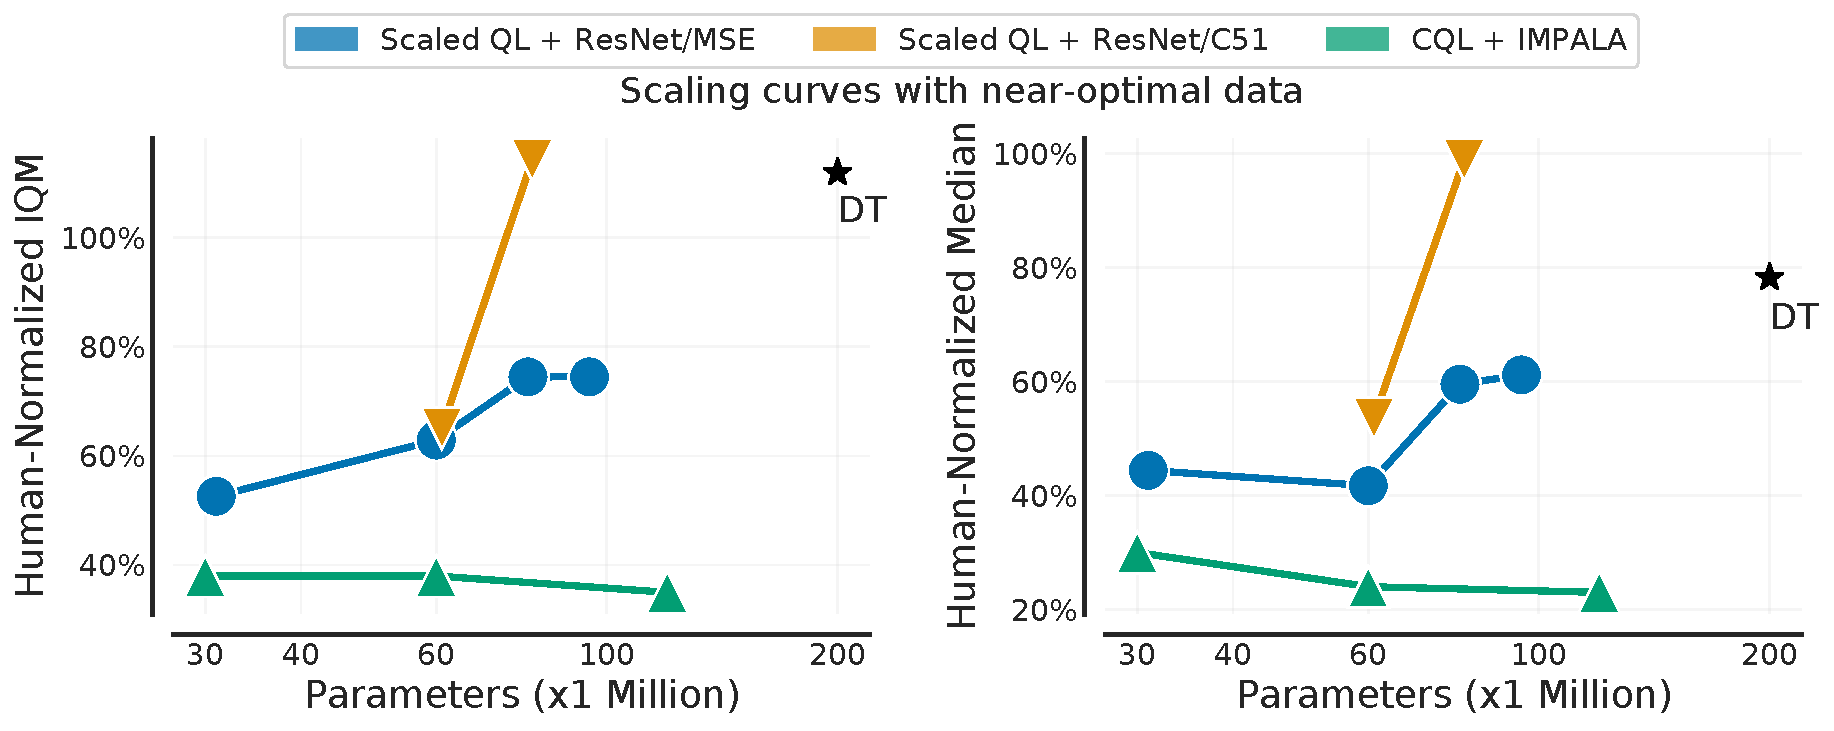
\includegraphics[width=0.75\linewidth]{chapters/scaled_ql/figures/scaling_plot_params_with_dt.pdf}
\vspace{-0.2cm}
\caption{\footnotesize{\textbf{Scaling trends for offline Q-learning.} Observe that while the performance of scaled QL instantiated with IMPALA architectures~\citep{espeholt2018impala} degrades as we increase model size, the performance of scaled QL utilizing the ResNets described in Section~\ref{sec:scaledql_method} continues to increase as model capacity increases. This is true for both an MSE-style TD error as well as for the categorical TD error used by C51 (which performs better on an absolute scale). The CQL + IMPALA performance numbers are from~\citep{lee2022multi}.}
}
\label{fig:scaling}
\vspace{-0.2cm}
\end{figure}

\vspace{-0.2cm}
\subsubsection{Does Offline Conservative Q-Learning Scale Favorably?}
\vspace{-0.2cm}
One of the primary goals of this chapter was to understand if scaled Q-learning is able to leverage the benefit of higher capacity architectures. Recently, \citet{lee2022multi} found that the performance of CQL with the IMPALA architecture does not improve with larger model sizes and may even degrade with larger model sizes. To verify if scaled Q-learning can address this limitation, we compare our value-based offline RL approach with a variety of model families: \textbf{(a)} IMPALA family~\citep{espeholt2018impala}: three IMPALA models with varying widths ($4, 8, 16$) whose performance numbers are taken directly from \citet{lee2022multi} (and was consistent with our preliminary experiments), 
%%AK: check if this is the standard naming or not?
\textbf{(b)} ResNet 34, 50, 101 and 152 from the ResNet family, modified to include group normalization and learned spatial embeddings.%, and \textbf{(c)} ViT-Base and ViT-Large from the vision transformer family, similar to decision transformers. 
These architectures include both small and large networks, spanning a wide range from 1M to 100M parameters. As a point of reference, we use the scaling trends of the multi-game decision transformer and BC approaches from \citet{lee2022multi}.
%%SL.9.27: if we don't end up including vit, make sure to revise the above discussion

Observe in Figure~\ref{fig:scaling} that the performance of scaled Q-learning improves as the underlying Q-function model size grows. Even though the standard mean-squared error formulation of TD error results in worse absolute performance than C51 (blue vs orange), for both of these versions, the performance of scaled Q-learning increases as the models become larger. This result indicates that value-based offline RL methods can scale favorably, and give rise to better results, but this requires carefully picking a model family. This also explains the findings from \citet{lee2022multi}: while this prior work observed that CQL with IMPALA scaled poorly as model size increases, they also observed that the performance of return-conditioned RL instantiated with IMPALA architectures also degraded with higher model sizes. Combined with the results in Figure~\ref{fig:scaling} above, this suggests that poor scaling properties of offline RL can largely be attributed to the choice of IMPALA architectures, which may not work well in general even for supervised learning methods (like return-conditioned BC).


\vspace{-0.2cm}
\subsubsection{Can Offline RL Learn Useful Initializations that Enable Fine-Tuning?}
\label{sec:ft_off_on}
\vspace{-0.2cm}

Next, we study how multi-task training on multiple games via scaled QL can learn general-purpose representations that can enable \emph{rapid} fine-tuning to new games. We study this question in two scenarios: fine-tuning to a new game via offline RL with a small amount of held-out data (1\% uniformly subsampled datasets from DQN-Replay~\citep{agarwal2019optimistic}), and finetuning to a new game mode via sample-efficient online RL initialized from our multi-game offline Q-function. For finetuning, we transfer the weights from the visual encoder and reinitialize the downstream feed-forward component (Figure~\ref{fig:overview}). For both of these scenarios, we utilize a ResNet101 Q-function trained via the methodology in Section~\ref{sec:scaledql_method}, using C51 and feature normalization.

\begin{figure}[t]
    \centering
    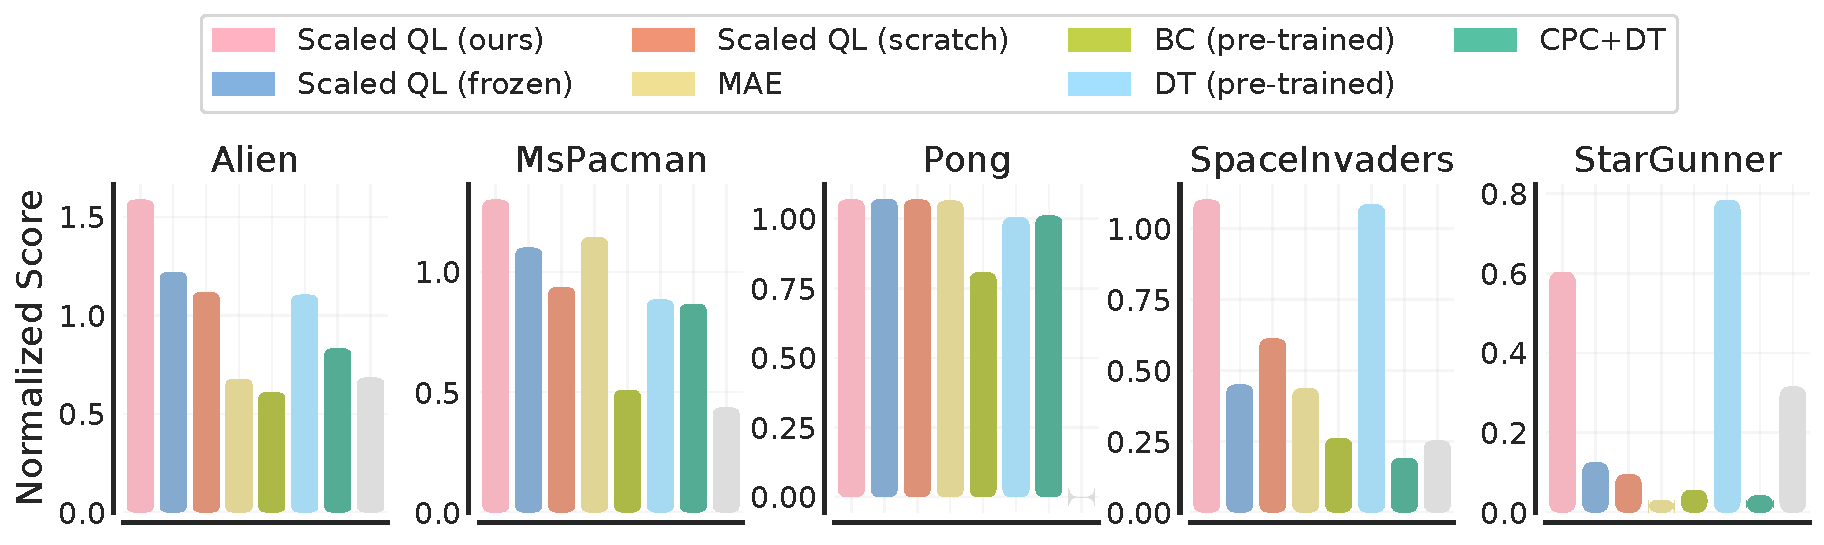
\includegraphics[width=0.99\linewidth]{chapters/scaled_ql/figures/offline_ft.pdf}
    \vspace{-0.25cm}
    \caption{\footnotesize{\textbf{Offline fine-tuning} performance on unseen games trained with 1\% of held-out game's data, measured in terms of DQN-normalized score, following \citep{lee2022multi}. On average, pre-training with scaled QL outperforms other methods by \textbf{82\%}. Furthermore, scaled QL improves over scaled QL (scratch) by 45\%, indicating that the representations learned by scaled QL during multi-game pre-training are useful for transfer. Self-supervised representation learning (CPC, MAE) alone does not attain good fine-tuning performance.}}
    \label{fig:offline_ft}
    \vspace{-0.3cm}
\end{figure}
%%AK: not having baselines para here, since the comparisons are different

\textbf{Scenario 1 (Offline fine-tuning)}: First, we present the results for fine-tuning in an offline setting: following the protocol from \citet{lee2022multi}, we use the pre-trained representations to rapidly learn a policy for a novel game using limited offline data (1\% of the experience of an online DQN run). In Figure~\ref{fig:offline_ft}, we present our results for offline fine-tuning on 5 games from \citet{lee2022multi}, \textsc{Alien, MsPacman, Space Invaders, StarGunner} and \textsc{Pong}, alongside the prior approach based on decision transformers (``DT (pre-trained)''), and fine-tuning using pre-trained representations learned from state-of-the-art self-supervised representation learning methods such as contrastive predictive coding (CPC)~\citep{oord2018representation} and masked autoencoders (MAE)~\citep{he2111masked}. For CPC performance, we use the baseline reported in \citet{lee2022multi}. MAE is a more recent self-supervised approach that we find generally outperformed CPC in this comparison. For MAE, we first pretrained a vision transformer~(ViT-Base)~\citep{dosovitskiy2020image} encoder with 80M parameters trained via a reconstruction loss on observations from multi-game Atari dataset and freeze the encoder weights as done in prior work~\citep{xiao2022masked}. 
Then, with this frozen visual encoder, we used the same feed forward architecture, Q-function parameterization, and training objective (CQL with C51) as scaled QL to finetune the MAE network. We also compare to baseline methods that do not utilize any multi-game pre-training (DT (scratch) and Scaled QL (scratch)). 

\textbf{Results.} Observe in Figure~\ref{fig:offline_ft} that multi-game pre-training via scaled QL leads to the best fine-tuning performance and improves over prior methods, including decision transformers trained from scratch. %, by XX\% in aggregate. 
Importantly, we observe \emph{positive transfer} to new games via scaled QL. Prior works~\citep{badia2020agent57}
running multi-game Atari (primarily in the online setting) have generally observed negative transfer across Atari games. We show for the first time that pre-trained representations from Q-learning enable positive transfer to novel games that significantly outperforms return-conditioned supervised learning methods and dedicated representation learning approaches.

\textbf{Scenario 2 (Online fine-tuning)}: Next, we study the efficacy of the learned representations in enabling online fine-tuning. While deep RL agents on ALE are typically trained on default game modes~(referred to as $m0d0$), we utilize new \emph{variants} of the ALE games designed to be challenging for humans~\citep{machado18sticky} for online-finetuning. We investigate whether multi-task training on the 40 default game variants can enable fast online adaptation to these never-before-seen variants. In contrast to offline fine-tuning (Scenario 1), this setting tests whether scaled QL can also provide a good initialization for online data collection and learning, for closely related but different tasks. Following \citet{farebrother2018generalization}, we use the same \emph{variants} investigated in this prior work: $\textsc{Breakout}$, $\textsc{Hero}$, and $\textsc{Freeway}$, which we visualize in Figure~\ref{fig:online_ft}~(left).
To disentangle the performance gains from multi-game pre-training and the choice of Q-function architecture, we compare to a baseline approach (``scaled QL (scratch)'') that utilizes an identical Q-function architecture as pre-trained scaled QL, but starts from a random initialization. As before, we also evaluate fine-tuning performance using the representations obtained via masked auto-encoder pre-training~\citep{he2111masked,xiao2022masked}. We also compare to a single-game DQN performance attained after training for 50M steps, $16\times$ more transitions than what is allowed for scaled QL, as reported by \citet{farebrother2018generalization}.

\textbf{Results}. Observe in Figure~\ref{fig:online_ft} that fine-tuning from the multi-task initialization learned by scaled QL significantly outperforms training from scratch as well as the single-game DQN run trained with \textbf{16x} more data. Fine-tuning with the frozen representations learned by MAE performs poorly, which we hypothesize is due to differences in game dynamics and subtle changes in observations, which must be accurately accounted for in order to learn optimal behavior~\citep{dean2022don}. Our results confirm that offline Q-learning can both effectively benefit from higher-capacity models and learn multi-task initializations that enable sample-efficient transfer to new games. 


\begin{figure}[t]
    \centering
        
\includegraphics[width=0.9\linewidth]{chapters/scaled_ql/figures/legend_online_ft.pdf}
        \vspace{-0.1cm}
        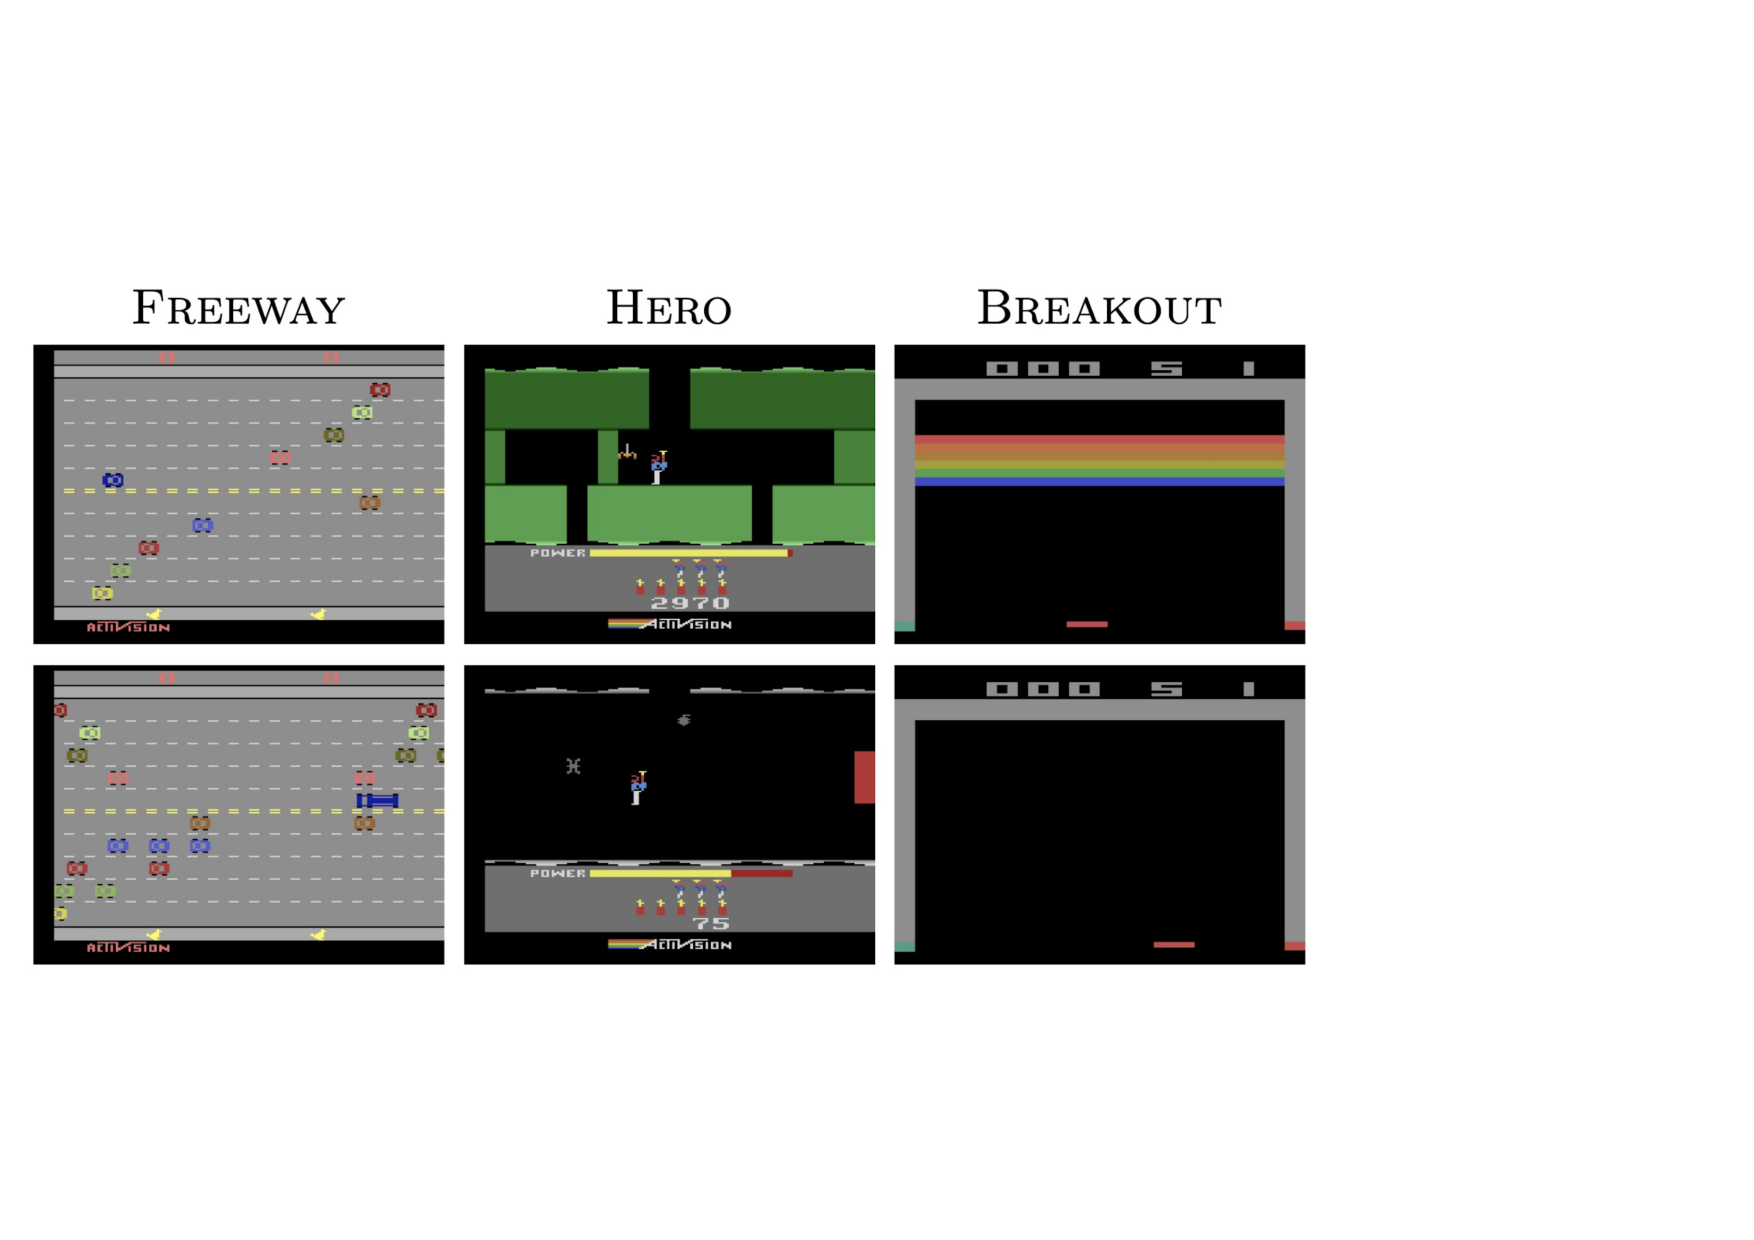
\includegraphics[width=0.35\linewidth]{chapters/scaled_ql/figures/atari_modes_3games.pdf}
        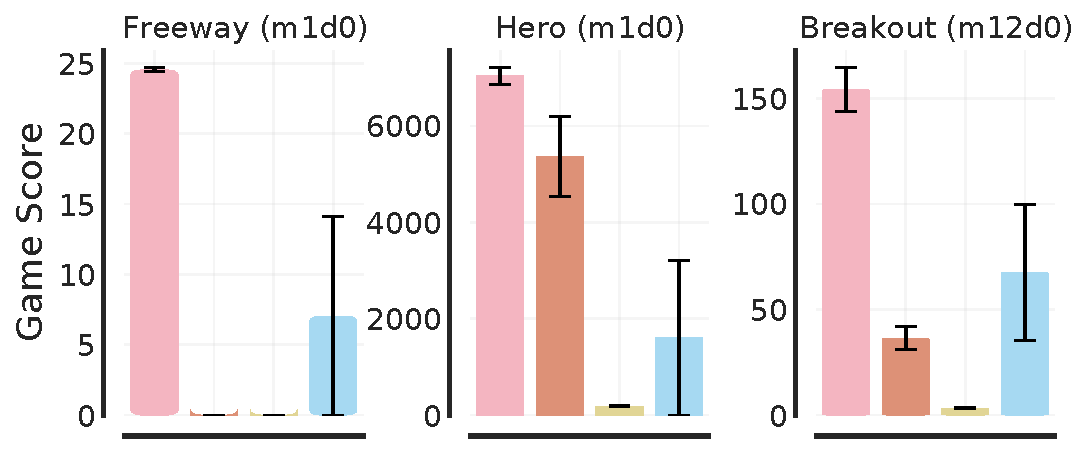
\includegraphics[width=0.5\linewidth]{chapters/scaled_ql/figures/online_ft_3_games.pdf}
    \vspace{-0.1cm}
    \caption{\footnotesize{\textbf{Online fine-tuning} results on unseen game \emph{variants}. \textbf{Left}. The top row shows default variants and the bottom row shows unseen variants evaluated for transfer: Freeway’s mode 1 adds buses, more vehicles, and increases velocity; Hero’s mode 1 starts the agent at level 5; Breakout’s mode 12 hides all bricks unless the ball has recently collided with a brick. \textbf{Right}. We fine-tune all methods except single-game DQN for 3M online frames (as we wish to test fast online adaptation). Error bars show minimum and maximum scores across 2 runs while the bar shows their average. Observe that scaled QL significantly outperforms learning from scratch and single-game DQN with 50M online frames. Furthermore, scaled QL also outperforms RL fine-tuning on representations learned using masked auto-encoders. See Figure~\ref{fig:lr_curves_online_ft} for learning curves.}}
    \label{fig:online_ft}
    \vspace{-0.5cm}
\end{figure}


\vspace{-0.25cm}
\subsubsection{Ablation Studies}
\label{sec:ablation}
\vspace{-0.25cm}

Finally, in this section we perform controlled ablation studies to understand how crucial the design decisions introduced in Section~\ref{sec:scaledql_method} are for the success of scaled Q-learning. In particular, we will attempt to understand the benefits of using C51 and feature normalization.

\textbf{MSE vs C51:} We ran scaled Q-learning with identical network architectures (ResNet 50 and ResNet 101), with both the conventional squared error formulation of TD error, and compare it to C51, which our main results utilize. Observe in Table~\ref{tab:ablation_mse} that C51 leads to much better performance for both ResNet 50 and ResNet 101 models. The boost in performance is the largest for ResNet 101, where C51 improves by over \textbf{39\%} as measured by median human-normalized score. This observation is surprising since prior work~\citep{agarwal2021deep} has shown that C51 performs on par with standard DQN with an Adam optimizer, which all of our results use. One hypothesis is that this could be the case as TD gradients would depend on the scale of the reward function, and hence some games would likely exhibit a stronger contribution in the gradient. This is despite the fact that our implementation of MSE TD-error already attempts to correct for this issue by applying the unitary scaling technique from \citep{kurin2022defense} to standardize reward scales across games. That said, we still observe that C51 performs significantly better.

\begin{table}[t]
    \centering
% \fontsize{8}{8}\selectfont
    \centering
    \vspace{-0.3cm}
    \caption{\footnotesize{\textbf{Performance of Scaled QL with the standard mean-squared TD-error and C51} in the offline 40-game setting aggregated by the median human-normalized score. Observe that for both ResNet 50 and ResNet 101, utilizing C51 leads to a drastic improvement in performance.}}% (as large as 39.4\% improvement on human-median normalized score with ResNet 101).}}
    \label{tab:ablation_mse}
    \vspace{0.1cm}
\resizebox{0.6\linewidth}{!}{\begin{tabular}{lcc}
\toprule
 & \textbf{Scaled QL (ResNet 50)} & \textbf{Scaled QL (ResNet 101)} \\
\midrule
\textbf{with MSE}  &  41.1\% & 59.5\%  \\
\midrule
\textbf{with C51}  & 53.5\% (+12.4\%) & 98.9\% (+39.4\%) \\
\bottomrule
\vspace{-0.25in}
\end{tabular}}
\end{table}


\textbf{Importance of feature normalization:} We ran small-scale experiments with and without feature normalization (Section~\ref{sec:scaledql_method}). In these experiments, we consider a multi-game setting with only 6 games: \textsc{Asterix}, \textsc{Breakout}, \textsc{Pong}, \textsc{SpaceInvaders}, \textsc{Seaquest}, and we train with the initial 20\% data for each game. We report aggregated median human-normalized score across the 6 games in Table~\ref{tab:ablation_dr3} for three different network architectures (ResNet 34, ResNet 50 and ResNet 101). Observe that the addition of feature normalization significantly improves performance for all the models. Motivated by this initial empirical finding, we used feature normalization in all of our main experiments. Overall, the above ablation studies validate the efficacy of the two key design decisions in this chapter. 
% However, there are several avenues for future investigation: 1) it is unclear if C51 works better because of the distributional formulation or the categorical representation and experiments with other distributional formulations could answer this question, 2) we did not extensively try alternate feature normalization schemes which may improve results. 

\begin{table}[ht]
    \centering
% \fontsize{8}{8}\selectfont
    \centering
    \vspace{-0.2cm}
    \caption{\footnotesize{\textbf{Performance of Scaled QL with and without feature normalization in the 6 game setting} reported in terms of the median human-normalized score. Observe that with models of all sizes, the addition of feature normalization improves performance.}}
    \label{tab:ablation_dr3}
    \vspace{0.1cm}
\resizebox{\linewidth}{!}{\begin{tabular}{lccc}
\toprule
 & \textbf{Scaled QL (ResNet 34)} & \textbf{Scaled QL (ResNet 50)} & \textbf{Scaled QL (ResNet 101)} \\
\midrule
\textbf{without feature normalization}  &  50.9\%  & 73.9\% & 80.4\%    \\
\midrule
\textbf{with feature normalization}  & 78.0\% (+28.9\%)  & 83.5\% (+9.6\%)  & 98.0\% (+17.6\%) \\
\bottomrule
\vspace{-0.2in}
\end{tabular}
}
\end{table}

\textbf{Additional ablations:} We also conducted ablation studies for the choice of the backbone architecture (spatial learned embeddings) in Appendix~\ref{app:backbone_ablation}, and observed that utilizing spatial embeddings is better. We also evaluated the performance of scaled QL without conservatism to test the importance of utilizing pessimism in our setting with diverse data in Appendix~\ref{app:no_pessimism}, and observe that pessimism is crucial for attaining good performance on an average. We also provide some scaling studies for another offline RL method (discrete BCQ) in Appendix~\ref{app:discrete_bcq}.


\iffalse

\section{Theoretical Analysis of \methodname\ }%and \AliasingProblemName}
\label{sec:analysis}

\textcolor{red}{This section goes away} A major challenge with value based RL methods, especially in the offline setting, is bootstrapping error accumulation, which refers to how sampling error increases when the value function itself is used to produce regression targets for temporal difference~(TD) error minimization.
In this section, we illustrate the benefits of \methodname\ by showing that given a set of features $\phi(\bs, \ba)$, the policy estimation error according to the Q$^\pi$-function learned from these features depends on $\simunnorm(\bs, \ba, \bs'; \phi)$. This indicates that explicitly minimizing $\simunnorm$, as done by \methodname, should result in lower error accumulation and more accurate estimates of policy return, and therefore more effective offline RL.
% In this section, we theoretically analyze the benefits of \methodname, by illustrating that the value of $\simunnorm$ directly affects bootstrapping error accumulation. By controlling $\simunnorm$, \methodname\ can reduce error accumulation and produce more accurate value estimates, thus improving offline RL.
%%SL.2.3: Slightly tweaked the above, but we could make it even mroe explicit, such as: can effectively reduce error accumulation. When combined with conservative value learning methods like CQL~\citep{}, we show that Q-functions learned with \methodname\ lower bound the true Q-function, but represent a tighter bound than those obtained with CQL alone. [or something like that]

%%SL.2.3: If 5.1 is the only subsection in Sec 5, then I don't think we need the subsection heading, we could just make the subsection title be the section title

Our goal is to show that training the Q-function with \methodname, which minimizes unnormalized feature similarities, results in a tighter bound on the true policy return when combined with a conservative offline RL algorithm, such as CQL~\citep{kumar2020conservative}. Intuitively, a tighter bound is attained because \methodname\ reduces the degree to which bootstrapping error accumulates. 
% compounds in temporal difference (bootstrapping) backups with finite datasets.
%%SL.2.3: I wonder if it might help to briefly mention something about bootstrap error before this, by way of motivation -- e.g., something like: A major challenge with TD-based RL, especially in the offline setting, is boootstrap error accumulation, which refers to how error increases when the value function itself is used to produce regression targets for Bellman error minimization.
Since we are primarily interested in the relationship between feature similarities and policy return estimates,
%%SL.2.1: I don't get it -- isn't the whole point to analyze feature learning? How can we analyze a regularizer on the features if the features are constant? Or does "linear function approximation" in this case mean something other than "features are constant"?
%%AK.2.3: Agreed, but I don't think we can analyze feature learning in the first place at all as of now. This is just aiming to obtain a groundtruth estimate of what properties will make learning better. 
%%SL.2.3: OK, after reading this a bit more carefully, what I *think* you meant to say here is more like this: We will show that, given a set of feature $whatever$, the policy estimation error according to the Q-function learned from these features depends on $sim(whatever)$. This indicates that explicitly minimizing this quantity should result in lower error accumulation and more accurate estimates of policy return, and therefore more effective reinforcement learning.
our analysis will focus on the linear function approximation setting, where we will characterize the values of $\simunnorm$ that lead to better estimates.

We assume a notion of realizability on the features $\phi(\bs,\ba)$. While conventional realizability refers to the true Q-function being representable in terms of the provided features, we use a significantly weaker assumption, which we term \emph{conservative realizability}, which only requires that a conservative estimate of the Q-function be realizable under features $\phi(\bs, \ba)$ as is the case with offline RL methods that learn lower-bounds on the value function~(\eg CQL) or pessimistically modify the reward function~\citep{?}.  
\begin{definition}[Conservative realizability]
Assume that the learned Q-function for any policy $\pi$ is parameterized as a linear function of features $\phi$: $Q_\phi(\bs, \ba) = {\bw}_\pi^T \phi(\bs,\ba)$. Then features $\phi(\bs, \ba)$ are said to be conservatively realizable with degree $\alpha$ against the behavior policy $\behavior$ if, there exists a function $f(\pi, \behavior, \phi)$ such that, $\forall~ \pi, \bs, \ba,~ Q^\phi(\bs, \ba) \geq Q_\pi(\bs, \ba) - \alpha f(\pi, \behavior, \phi)(\bs, \ba)$, and f satisfies: $f(\behavior, \behavior, \phi) = 0$, $f(\pi, \behavior, \phi) > 0 ~\forall~ \pi \neq \behavior$.  
\end{definition}

\begin{theorem}[\methodname\ attains tighter bound on return]
\label{thm:return_bound}
Suppose the Q-function is given by $Q_\phi(\bs, \ba) = \bw^T \phi(\bs, \ba)$ and for any policy $\pi \in \Pi$, representation $\phi$ is conservatively realizable. 
Given an offline dataset $\data$ of size $N$, let $\Sigma_\data = \sum_{i=1}^N \phi(\bs_i, \ba_i) \phi(\bs_i, \ba_i)^T$ be the covariance matrix of the dataset features and assume $\sigma_{\min}(\Sigma_\data) := 1/c >0$. In this case, running off-policy evaluation for a given policy $\pi$ via fitted Q-evaluation~\citep{} yields $\hat{\bw}_\pi$ such that the optimal $\bw_\pi$ and $\hat{\bw}^\pi$ satisfy with high probability $\geq 1-\delta$ that
\begin{equation*}
    ||\bw_\pi - \hat{\bw}_\pi||_2 \leq \frac{C_{\delta, \gamma} c}{1 - \gamma c \left(\E_{\bs, \ba, \bs' \sim \data}[\simunnorm(\bs, \ba, \bs')] \right)},
%%AK.2.3: this should technically have an additional term that subtracts the function value f
\end{equation*}
where $C_{\delta, \gamma}$ is a constant depending on $\delta, \gamma$. Thus, the expected policy return under initial state-action distribution $\rho(\bs_0, \ba)$, $\hat{J}_\phi(\pi) := \E_{\bs_0 \sim \rho, \ba \sim \pi}[Q_\phi(\bs, \ba)]$, and the actual policy return, $J(\pi)$, satisfies
\begin{equation*}
    \left\vert \hat{J}_\phi(\pi) - J(\pi) \right\vert \leq ||\Phi_\rho||_2 ||\bw_\pi - \hat{\bw}_\pi||_2,
%%AK.1.31: see jamboard and decide whether to write this in terms of \hat{w}^\pi directly or the return of the policy. 
\end{equation*}
where $\phi_\rho$ denotes the expected feature vector on the initial state distribution $\bs_0 \sim \rho$.
\end{theorem}
This result clearly indicates that $\E_{\bs, \ba, \bs' \sim \mathcal{D}}[\simunnorm(\bs, \ba, \bs')]$ directly controls the amount of error accumulated in the weight vector $\hat{\bw}^\pi$ as a result of bootstrapping. Since $\hat{J}(\pi)$ is closer to $J(\pi)$ when the expected unnormalized similarity is small, optimizing features via \methodname\ to directly minimize this quantity controls the tightness or accuracy of the return estimate $\hat{J}(\pi)$. When applied on top of a conservative offline RL method, such as CQL, which satisfies the conservative realizability condition with $f=$, \methodname\ provides tighter return estimates by reducing the amount of error accumulated during bootstrapping,
%%AK.2.3: fill this in
%%AK.1.31: is it unclear how stable came into the picture?
%%SL.2.1: Yes, there is a missing link between "tighter bound" and "robust and stable" (also, try to avoid the word "robust" as it is easy to misunderstand to mean robust control -- i.e., robust to perturbations)

\fi

\iffalse

\subsection{Why Does \AliasingProblemName\ Happen?}
\label{sec:why_does_aliasing_happen}
%%AK.2.1: this section is not edited yet
%%SL.2.1: It's also unclear how this section relates to the previous one...

Finally, we aim to theoretically understand the cause behind the feature aliasing problem. It is evident from Figure ?? that feature aliasing only persists as long as bootstrapping (i.e., TD error) is used and supervised regression does not exhibit this issue. We will now show that feature aliasing is caused by \emph{compounding} of the implicit regularization of gradient descent towards producing simple ``min-norm'' solutions in non-linear networks when bootstrapping is used.
%%SL.1.26: The above sentence reads kind of backwards, maybe we can ease the reader into this by first explaining what this compounding is, and then what it has to do with feature aliasing
Similar to other works in supervised learning~\citep{savarese2019infinite}, operates in the setting with wide 2-layer ReLU networks.
%%SL.1.26: Above sentence is malformed somehow? Maybe a missing word or typo?
Here, the Q-function is given by:
\begin{equation}
    Q(\bs, \ba) = \sum_{i=1}^{n} w^i_2 \underbrace{\left[ [\bs, \ba]^T \bw^i_1 + b^i_1  \right]_{+}}_{:= \phi^i(\bs, \ba)} +~ b^i_2.
\label{eqn:relu_q}
%%SL.1.26: it's not immediately obvious why "here" the q-function is given by this -- are you just writing the equation for last layer features? it's kind of not clear where this comes from
\end{equation}
The $i$-th dimension of the features $\phi(\bs, \ba)$ is marked in Equation~\ref{eqn:relu_q}. Now, we define the ``min-norm'' solution for bootstrapping that is equivalent to the solution found by gradient descent on the TD error objective on a finite dataset, and the rest of our analysis will characterize properties of this optimization problem with bootstrapping.
%%SL.1.26: I'm actually having a lot of difficulty following the paragraph above or what it is trying to say. Perhaps it would help to add a bit more discussion for why we care about min-norm solutions, and what this has to do with gradient descent and bootstrapping
\begin{definition}[Min-norm solution]
\label{eqn:min_norm}
The min-norm solution for parameters $\bw_2$, $\bw_1$, $b_1$ and $b_2$ of the two-layer ReLU network in a given iteration of TD-learning for off-policy evaluation of a given policy $\pi$ is given by:
\begin{align*}
    \min_{\bw_1, \bw2, b_1, b_2}~~ & ||\bw_2||_1 \\
    \text{s.t.}~~ Q_\theta(\bs_i, \ba_i) &= r_i + \gamma \E_{\pi}[Q_{\bar{\theta}}(\bs'_i, \ba')]~~ \forall~ i \in [\data],\\
    & ||\bw^i_1||_2 = 1~~ \forall~ i \in [1,\cdots, n].
\end{align*}
\end{definition}
%%SL.1.26: this definition comes across as a bit arbitrary. Maybe a bit more context would help. Why is the norm of w_1 equal to 1? I can guess the intuition (I'm guessing you're trying to limit the Lipschitz constant of the features, so that any statement about the norm of the last-layer weights actually means something about the overall function), but this is not really explained, so many readers will see this as pretty ad hoc and wonder what this has to do with reality.
%%AK.1.24: also need to discuss early stopping somewhere -- else the datapoint thing is a constraint, and one could always fit it and something bad will may never happen. Also, check if we need to include the biases b_1 and b_2 in the optimization objective or not? 
Here, we  use $\bar{\theta}$ to denote the target Q-network parameters (which is equal to the original Q-network from the previous iteration but is held fixed). We will denote the features of this target network for a state-action tuple $(\bs, \ba)$ as $\bar{\phi}(\bs, \ba)$.
Having covered the optimization problem, we now prove in Theorem~\ref{thm:bootstrapping} that training with bootstrapping is the primary reason behind the feature aliasing problem. We show this under two separate scenarios, both of which are likely to arise in offline RL settings with TD-learning.
%%SL.1.26: Kind of unclear what any of this has to do with Definition 2
The first scenario arises when the magnitude of the Q-value, $Q_{\theta}(\bs, \ba)$ is large compared to the magnitude of the reward $r$. This is expected in scenarios with completely positive or negative reward functions and limited data, when the Q-function erroneously overestimates or underestimates intermediately during training.
%%SL.1.26: This sounds pretty ad hoc, can you state this more precisely? I think reward is positive is fine, but it looks ad-hoc if you bring it up informally here like this (but it's also not that important I think...)
The second scenario comes into effect when the policy $\pi$ is quite different
%%SL.1.26: again, this comes across as vague and imprecise, can you state this more precisely somehow?
from the behavior policy $\pi_\beta$, where target Q-values are evaluated on unseen state-action pairs, and they are not trained on.
This is common in several OPE problems, offline RL settings with limited data or when standard off-policy RL algorithms are used.
%%SL.1.26: I don't think it's more common in OPE problems, but it's fine to just say: this is often the case in offline RL, since the goal of offline RL methods is to learn policies that improve over the behavior policy, and therefore differ from it [or something like that]
We formally state these conditions as Scenarios~\ref{assumption:magnitude} and \ref{assumption:ood} and show in Theorem~\ref{thm:bootstrapping} that features are aligned under these conditions.

\begin{assumption}[Magnitude difference]
\label{assumption:magnitude}
Without loss of generality,
%%SL.1.26: maybe just bring in this assumption earlier (e.g., in the preliminaries) -- something like, in our analysis we will assume that the reward are always positive. This assumption can be made without loss of generality if the rewards are guaranteed to be finite, because...
assume that the reward function $r(\bs, \ba)$ is always positive. Then, we assume that $\gamma$ is sufficiently close to 1 and the current Q-function is such that 
\begin{equation*}
    Q_\theta = r + \gamma \hat{\gT}^\pi Q_\theta  ~\approx~ Q_\theta = \varepsilon + \gamma \hat{\gT}^\pi Q_\theta,~~~ \varepsilon \sim \gN(0, I).
%%AK.1.24: basically, we want to say that now the reward function doesnt matter, it is just as good as noise. The eps sampled from N(O, I) may appear a bit odd, we need not have it. I just put it to signify that the term is just noise.
\end{equation*}
\end{assumption}
%%SL.1.26: Perhaps for these assumptions, it would be a bit clearer to state the assumption first, then the intuition, instead of putting the intuition first like you did above -- otherwise the intuition coming before the definition makes it sound imprecise and a bit clumsy

\begin{assumption}[OOD actions]
\label{assumption:ood}
Assume that the policy $\pi(\ba|\bs)$ is such that for any state-action tuple $\bs \in \mathcal{D}, \ba \sim \pi(\cdot|\bs)$, $\pi_\beta(\ba|\bs) < \varepsilon$.  
%%SL.1.26: for *any*? meaning all actions have low probability? or just some (i.e., "there exists")? If this is for all actions, that seems like a pretty unusual situation
%%AK.1.24: compute the form for epsilon here.... it will depend on the dataset. Also need to relax the for all condition... can be done when analyzing under early stopping
\end{assumption}

\begin{theorem}
\label{thm:bootstrapping}
Assume at least one of scenarios~\ref{assumption:magnitude} and \ref{assumption:ood} holds. Let the feature representation of the target Q-network $Q_{\bar{\theta}}$ be denoted as $\bar{\phi}$. Then, solving the min-norm problem (Definition~\ref{eqn:min_norm}) produces $\phi$ such that, for all $(\bs, \ba, r, \bs') \in \mathcal{D}$, 
\begin{equation*}
     \simunnorm(\bs, \ba, \bs'; \phi) > \simunnorm(\bs, \ba, \bs'; \bar{\phi}).
\end{equation*}
\end{theorem}
%%SL.1.26: It's not clear to me what the significance of this is for two reasons: First, are we solving the min-norm problem? I guess you were going to argue that this is what we're doing because of bootstrap, but I don't see this made explicit anywhere. Second, why is having the cos^2 increase a bad thing? That does not prove that it will actually be large, or that anything bad will actually happen.
A proof can be found in Appendix ??. This key proof idea is that, whenever the TD error either uses target values from unseen state-action tuples or when the magnitude of Q-values is sufficient to overpower the reward signal, Problem~\ref{eqn:min_norm} is effectively under-constrained. In this case, an optimal solution will align state-action features, as doing this also minimizes $||\bw_2||_1$, which is the objective in Problem~\ref{eqn:min_norm}. Before moving on to our method, which attempts to mitigate the feature aliasing issue, we discuss how these results relate to recent work on lower bounds for offline RL.
%%AK.1.26: one thing that is missing here is that we do not talk about the recursiveness of the argument: since our theory so far depends on two scenarios, we need to show that once aliasing happens one of the two scenarios still remains, so that aliasing happens more again, and so on. But maybe that's hard. What do you guys think?
%%SL.1.26: Yeah, I see your point. I think maybe the bigger issue is that it's not clear why showing that current network aliasing between time steps is worse than target aliasing between time steps is actually equivalent to the original claims, which talk about aliasing between current and target networks. I think the reason is that a ~ beta and a' ~ pi, but this is not made explicit, and I think most readers won't get it. It's also not clear if proving that this increases like this actually proves that it gets bad (it might asymptote), can you make a more asymptotic argument somehow?

\fi


% \vspace{-0.2cm}
\subsection{Experimental Evaluation}
\label{sec:scaling_exps}
\vspace{-0.2cm}

\begin{figure}[t]
    \centering
    \begin{minipage}{0.65\linewidth}
 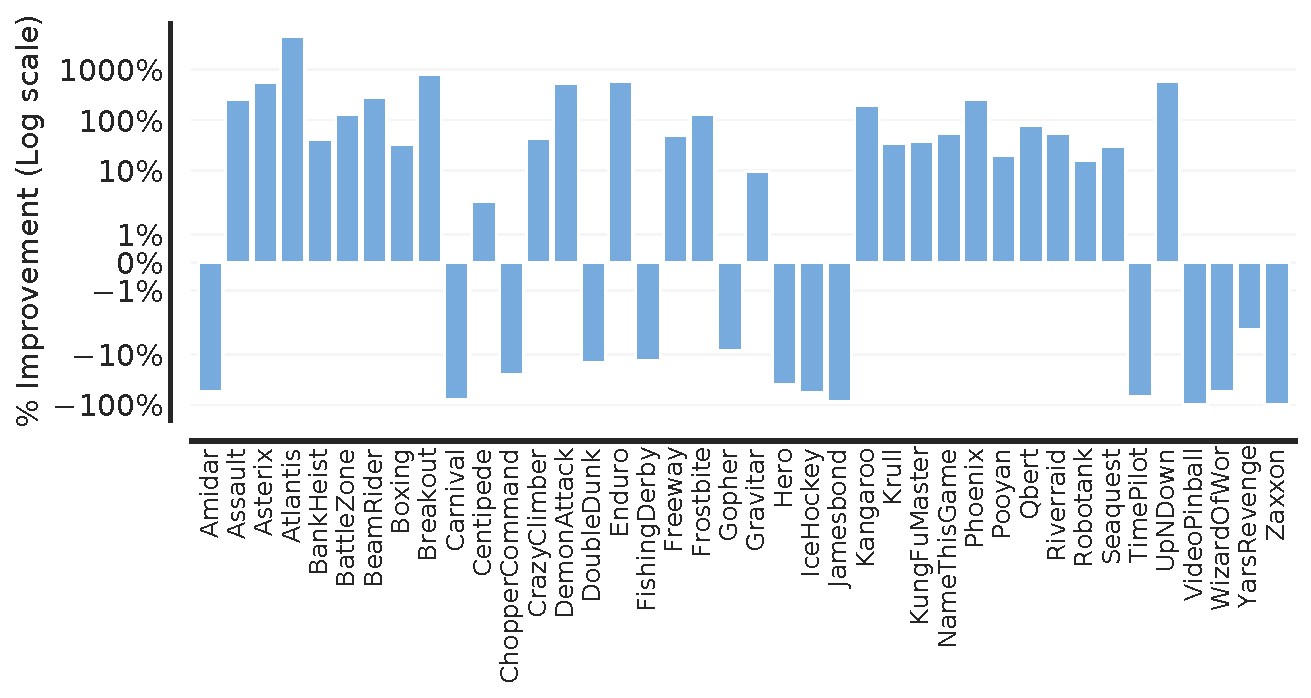
\includegraphics[width=\linewidth]{chapters/scaled_ql/figures/percent_improvement_over_DT.pdf}
    \end{minipage}
    \hfill
    \begin{minipage}{0.34\linewidth}
    \vspace{-0.2cm}
 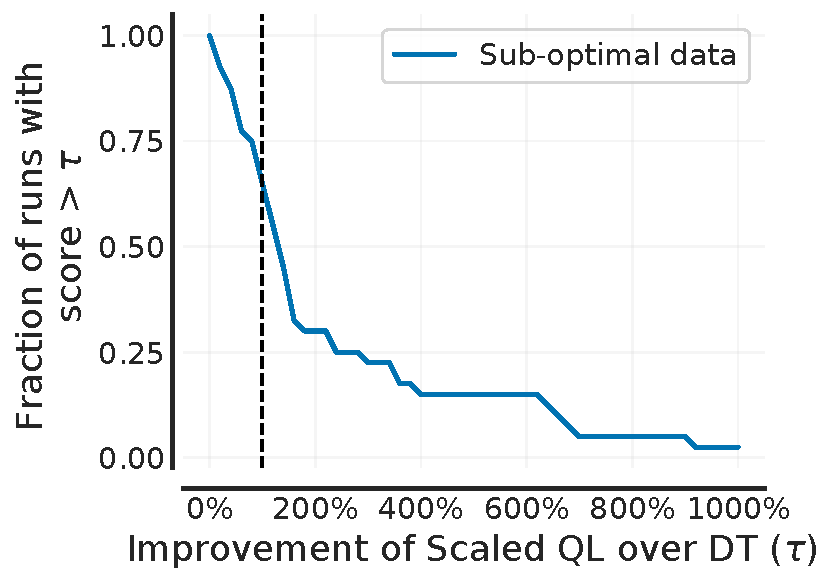
\includegraphics[width=\linewidth]{chapters/scaled_ql/figures/pp_profile_ql_dt.pdf}
    \end{minipage}
    \vspace{-0.4cm}
    \caption{\textbf{Comparing Scaled QL to DT} on all training games on the sub-optimal dataset.}
    \label{fig:percent_improvement}
    \vspace{-0.5cm}
\end{figure}

In our experiments, we study how our approach, scaled Q-learning, can simultaneously learn from sub-optimal and optimal data collected from 40 different Atari games. 
We compare the resulting multi-task policies to behavior cloning~(BC) with same architecture as scaled QL, and the prior state-of-the-art method based on decision transformers (DT)~\citep{chen2021decision}, which utilize return-conditioned supervised learning with large transformers~\citep{lee2022multi}, and have been previously proposed for addressing this task. 
We also study the efficacy of the multi-task initialization produced by scaled Q-learning in facilitating rapid transfer to new games via both offline and online fine-tuning, in comparison to state-of-the-art self-supervised representation learning methods and other prior approaches. Our goal is to answer the following questions: \textbf{(1)} How do our proposed design decisions impact performance scaling with high-capacity models?, \textbf{(2)} Can scaled QL more effectively leverage higher model capacity compared to na\"ive instantiations of Q-learning?, \textbf{(3)} Do the representations learned by scaled QL transfer to new games? We will answer these questions in detail through multiple experiments in the coming sections, but we will first summarize our main results below.


\textbf{Main empirical findings.} Our main results are summarized in Figures~\ref{fig:suboptimal_offline} and \ref{fig:main_results}. These figures show the performance of scaled QL, multi-game decision transformers~\citep{lee2022multi} (marked as ``DT''), a prior method based on supervised learning via return conditioning, and standard behavioral cloning baselines (marked as ``BC'') in the two settings discussed previously, where we must learn from: (i) near optimal data, and (ii) sub-optimal data obtained from the initial 20\% segment of the replay buffer (see our discussion about the problem setup). See Figure~\ref{fig:percent_improvement} for a direct comparison between DT and BC.


\begin{wrapfigure}{r}{0.5\linewidth}
    \vspace{-0.5cm}
    \centering
    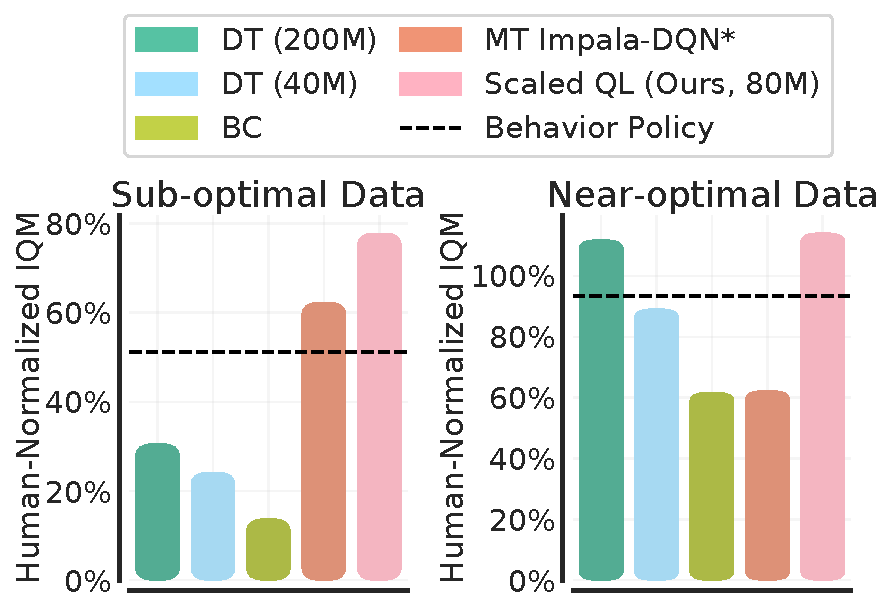
\includegraphics[width=0.95\linewidth]{chapters/scaled_ql/combnined_data_results_iqm.pdf}
    \vspace{-0.25cm}
    \caption{\footnotesize{\textbf{Offline scaled conservative Q-learning vs other prior methods} with near-optimal data and sub-optimal data. Scaled QL outperforms the best DT model, attaining an IQM human-normalized score of \textbf{114.1\%} on the near-optimal data and \textbf{77.8\%} on the sub-optimal data, compared to 111.8\% and 30.6\% for DT, respectively.}}
    \label{fig:main_results}
    \vspace{-0.5cm}
\end{wrapfigure}

In the more challenging sub-optimal data setting, scaled QL attains a performance of \textbf{77.8\%} IQM human-normalized score, although trajectories in the sub-optimal training dataset only attain 51\% IQM human-normalized score. Scaled QL also outperforms the prior DT approach by \textbf{2.5 times} on this dataset, even though the DT model has more than twice as many parameters and uses data augmentation, compared to scaled QL. 

In the $2^{nd}$ setting with near-optimal data, where the training dataset already contains expert trajectories, scaled QL with 80M parameters still outperforms the DT approach with 200M parameters, although the gap in performance is small (3\% in IQM performance, and 20\% on median performance). 
Overall, these results show that scaled QL is an effective approach for learning from large multi-task datasets, for a variety of data compositions including sub-optimal datasets, where we must stitch useful segments of suboptimal trajectories to perform well, and near-optimal datasets, where we should attempt to mimic the best behavior in the offline dataset. 

To the best of our knowledge, these results represent the largest performance improvement over the average performance in the offline dataset on such a challenging problem. We will now present experiments that show that offline Q-learning scales and generalizes.

\begin{figure}[h]
\centering
\vspace{-0.2cm}
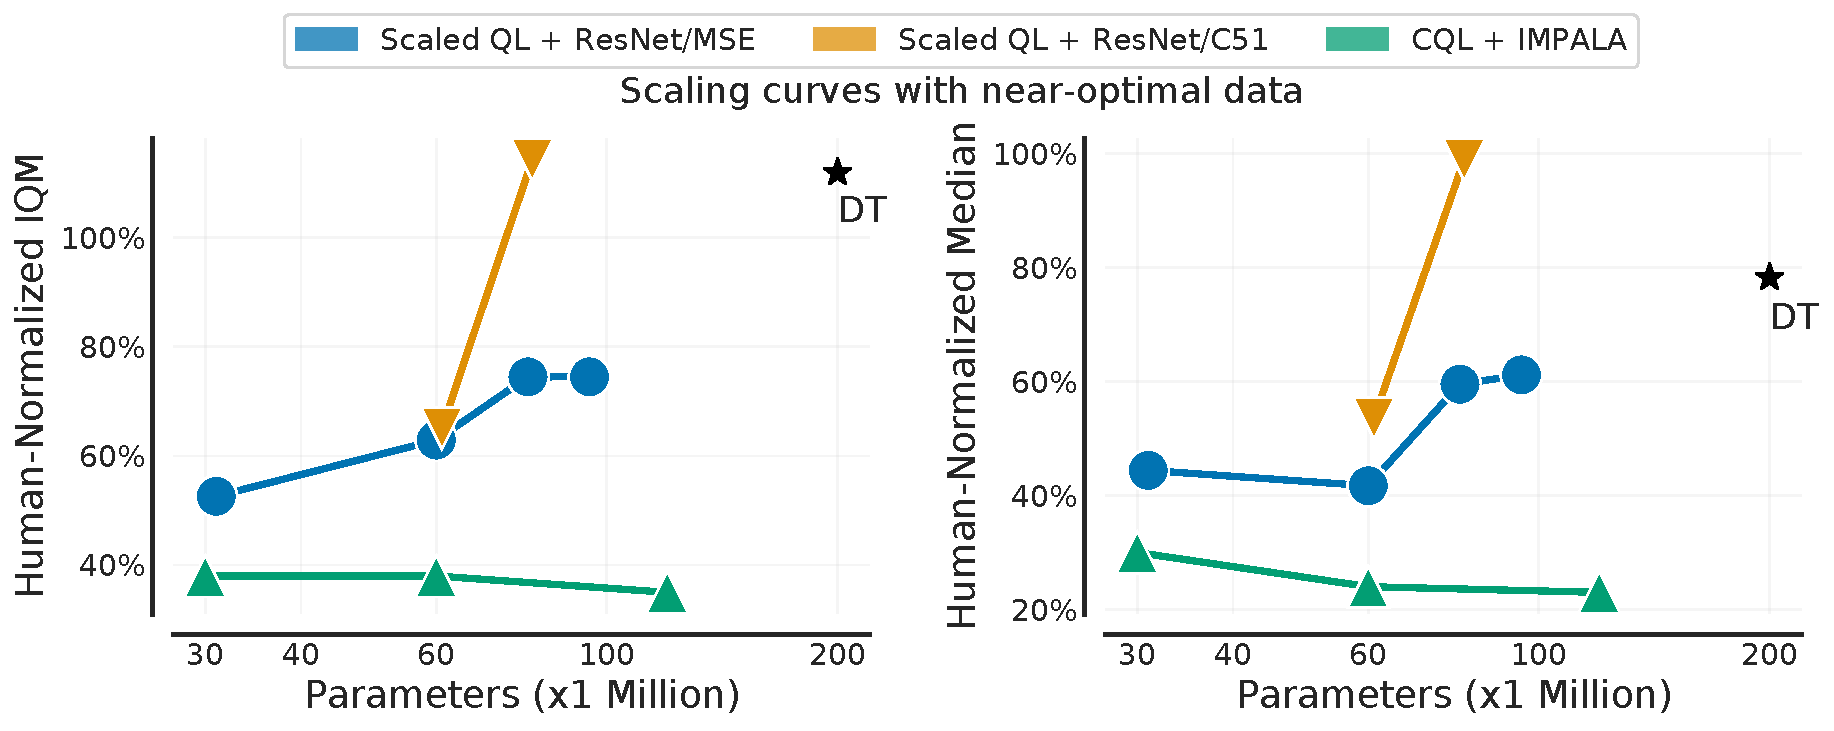
\includegraphics[width=0.75\linewidth]{chapters/scaled_ql/figures/scaling_plot_params_with_dt.pdf}
\vspace{-0.2cm}
\caption{\footnotesize{\textbf{Scaling trends for offline Q-learning.} Observe that while the performance of scaled QL instantiated with IMPALA architectures~\citep{espeholt2018impala} degrades as we increase model size, the performance of scaled QL utilizing the ResNets described in Section~\ref{sec:scaledql_method} continues to increase as model capacity increases. This is true for both an MSE-style TD error as well as for the categorical TD error used by C51 (which performs better on an absolute scale). The CQL + IMPALA performance numbers are from~\citep{lee2022multi}.}
}
\label{fig:scaling}
\vspace{-0.2cm}
\end{figure}

\vspace{-0.2cm}
\subsubsection{Does Offline Conservative Q-Learning Scale Favorably?}
\vspace{-0.2cm}
One of the primary goals of this chapter was to understand if scaled Q-learning is able to leverage the benefit of higher capacity architectures. Recently, \citet{lee2022multi} found that the performance of CQL with the IMPALA architecture does not improve with larger model sizes and may even degrade with larger model sizes. To verify if scaled Q-learning can address this limitation, we compare our value-based offline RL approach with a variety of model families: \textbf{(a)} IMPALA family~\citep{espeholt2018impala}: three IMPALA models with varying widths ($4, 8, 16$) whose performance numbers are taken directly from \citet{lee2022multi} (and was consistent with our preliminary experiments), 
%%AK: check if this is the standard naming or not?
\textbf{(b)} ResNet 34, 50, 101 and 152 from the ResNet family, modified to include group normalization and learned spatial embeddings.%, and \textbf{(c)} ViT-Base and ViT-Large from the vision transformer family, similar to decision transformers. 
These architectures include both small and large networks, spanning a wide range from 1M to 100M parameters. As a point of reference, we use the scaling trends of the multi-game decision transformer and BC approaches from \citet{lee2022multi}.
%%SL.9.27: if we don't end up including vit, make sure to revise the above discussion

Observe in Figure~\ref{fig:scaling} that the performance of scaled Q-learning improves as the underlying Q-function model size grows. Even though the standard mean-squared error formulation of TD error results in worse absolute performance than C51 (blue vs orange), for both of these versions, the performance of scaled Q-learning increases as the models become larger. This result indicates that value-based offline RL methods can scale favorably, and give rise to better results, but this requires carefully picking a model family. This also explains the findings from \citet{lee2022multi}: while this prior work observed that CQL with IMPALA scaled poorly as model size increases, they also observed that the performance of return-conditioned RL instantiated with IMPALA architectures also degraded with higher model sizes. Combined with the results in Figure~\ref{fig:scaling} above, this suggests that poor scaling properties of offline RL can largely be attributed to the choice of IMPALA architectures, which may not work well in general even for supervised learning methods (like return-conditioned BC).


\vspace{-0.2cm}
\subsubsection{Can Offline RL Learn Useful Initializations that Enable Fine-Tuning?}
\label{sec:ft_off_on}
\vspace{-0.2cm}

Next, we study how multi-task training on multiple games via scaled QL can learn general-purpose representations that can enable \emph{rapid} fine-tuning to new games. We study this question in two scenarios: fine-tuning to a new game via offline RL with a small amount of held-out data (1\% uniformly subsampled datasets from DQN-Replay~\citep{agarwal2019optimistic}), and finetuning to a new game mode via sample-efficient online RL initialized from our multi-game offline Q-function. For finetuning, we transfer the weights from the visual encoder and reinitialize the downstream feed-forward component (Figure~\ref{fig:overview}). For both of these scenarios, we utilize a ResNet101 Q-function trained via the methodology in Section~\ref{sec:scaledql_method}, using C51 and feature normalization.

\begin{figure}[t]
    \centering
    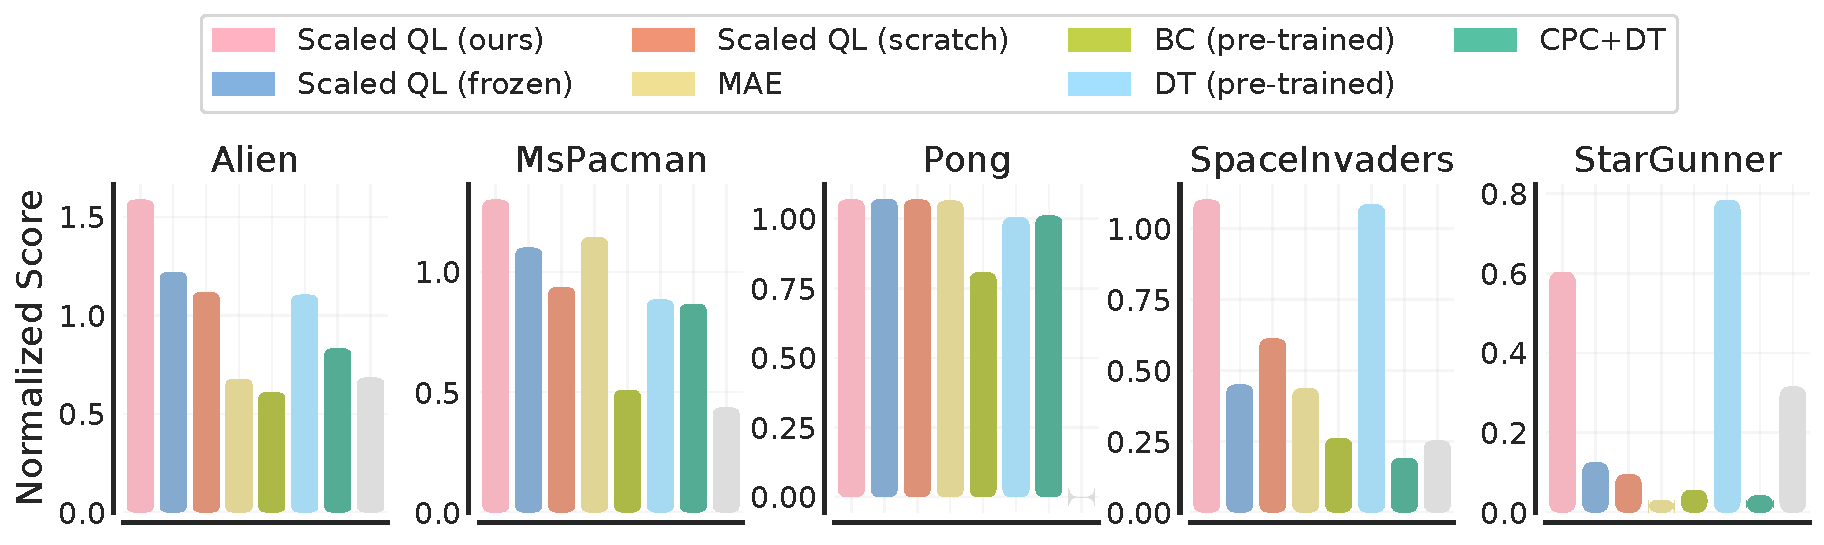
\includegraphics[width=0.99\linewidth]{chapters/scaled_ql/figures/offline_ft.pdf}
    \vspace{-0.25cm}
    \caption{\footnotesize{\textbf{Offline fine-tuning} performance on unseen games trained with 1\% of held-out game's data, measured in terms of DQN-normalized score, following \citep{lee2022multi}. On average, pre-training with scaled QL outperforms other methods by \textbf{82\%}. Furthermore, scaled QL improves over scaled QL (scratch) by 45\%, indicating that the representations learned by scaled QL during multi-game pre-training are useful for transfer. Self-supervised representation learning (CPC, MAE) alone does not attain good fine-tuning performance.}}
    \label{fig:offline_ft}
    \vspace{-0.3cm}
\end{figure}
%%AK: not having baselines para here, since the comparisons are different

\textbf{Scenario 1 (Offline fine-tuning)}: First, we present the results for fine-tuning in an offline setting: following the protocol from \citet{lee2022multi}, we use the pre-trained representations to rapidly learn a policy for a novel game using limited offline data (1\% of the experience of an online DQN run). In Figure~\ref{fig:offline_ft}, we present our results for offline fine-tuning on 5 games from \citet{lee2022multi}, \textsc{Alien, MsPacman, Space Invaders, StarGunner} and \textsc{Pong}, alongside the prior approach based on decision transformers (``DT (pre-trained)''), and fine-tuning using pre-trained representations learned from state-of-the-art self-supervised representation learning methods such as contrastive predictive coding (CPC)~\citep{oord2018representation} and masked autoencoders (MAE)~\citep{he2111masked}. For CPC performance, we use the baseline reported in \citet{lee2022multi}. MAE is a more recent self-supervised approach that we find generally outperformed CPC in this comparison. For MAE, we first pretrained a vision transformer~(ViT-Base)~\citep{dosovitskiy2020image} encoder with 80M parameters trained via a reconstruction loss on observations from multi-game Atari dataset and freeze the encoder weights as done in prior work~\citep{xiao2022masked}. 
Then, with this frozen visual encoder, we used the same feed forward architecture, Q-function parameterization, and training objective (CQL with C51) as scaled QL to finetune the MAE network. We also compare to baseline methods that do not utilize any multi-game pre-training (DT (scratch) and Scaled QL (scratch)). 

\textbf{Results.} Observe in Figure~\ref{fig:offline_ft} that multi-game pre-training via scaled QL leads to the best fine-tuning performance and improves over prior methods, including decision transformers trained from scratch. %, by XX\% in aggregate. 
Importantly, we observe \emph{positive transfer} to new games via scaled QL. Prior works~\citep{badia2020agent57}
running multi-game Atari (primarily in the online setting) have generally observed negative transfer across Atari games. We show for the first time that pre-trained representations from Q-learning enable positive transfer to novel games that significantly outperforms return-conditioned supervised learning methods and dedicated representation learning approaches.

\textbf{Scenario 2 (Online fine-tuning)}: Next, we study the efficacy of the learned representations in enabling online fine-tuning. While deep RL agents on ALE are typically trained on default game modes~(referred to as $m0d0$), we utilize new \emph{variants} of the ALE games designed to be challenging for humans~\citep{machado18sticky} for online-finetuning. We investigate whether multi-task training on the 40 default game variants can enable fast online adaptation to these never-before-seen variants. In contrast to offline fine-tuning (Scenario 1), this setting tests whether scaled QL can also provide a good initialization for online data collection and learning, for closely related but different tasks. Following \citet{farebrother2018generalization}, we use the same \emph{variants} investigated in this prior work: $\textsc{Breakout}$, $\textsc{Hero}$, and $\textsc{Freeway}$, which we visualize in Figure~\ref{fig:online_ft}~(left).
To disentangle the performance gains from multi-game pre-training and the choice of Q-function architecture, we compare to a baseline approach (``scaled QL (scratch)'') that utilizes an identical Q-function architecture as pre-trained scaled QL, but starts from a random initialization. As before, we also evaluate fine-tuning performance using the representations obtained via masked auto-encoder pre-training~\citep{he2111masked,xiao2022masked}. We also compare to a single-game DQN performance attained after training for 50M steps, $16\times$ more transitions than what is allowed for scaled QL, as reported by \citet{farebrother2018generalization}.

\textbf{Results}. Observe in Figure~\ref{fig:online_ft} that fine-tuning from the multi-task initialization learned by scaled QL significantly outperforms training from scratch as well as the single-game DQN run trained with \textbf{16x} more data. Fine-tuning with the frozen representations learned by MAE performs poorly, which we hypothesize is due to differences in game dynamics and subtle changes in observations, which must be accurately accounted for in order to learn optimal behavior~\citep{dean2022don}. Our results confirm that offline Q-learning can both effectively benefit from higher-capacity models and learn multi-task initializations that enable sample-efficient transfer to new games. 


\begin{figure}[t]
    \centering
        
\includegraphics[width=0.9\linewidth]{chapters/scaled_ql/figures/legend_online_ft.pdf}
        \vspace{-0.1cm}
        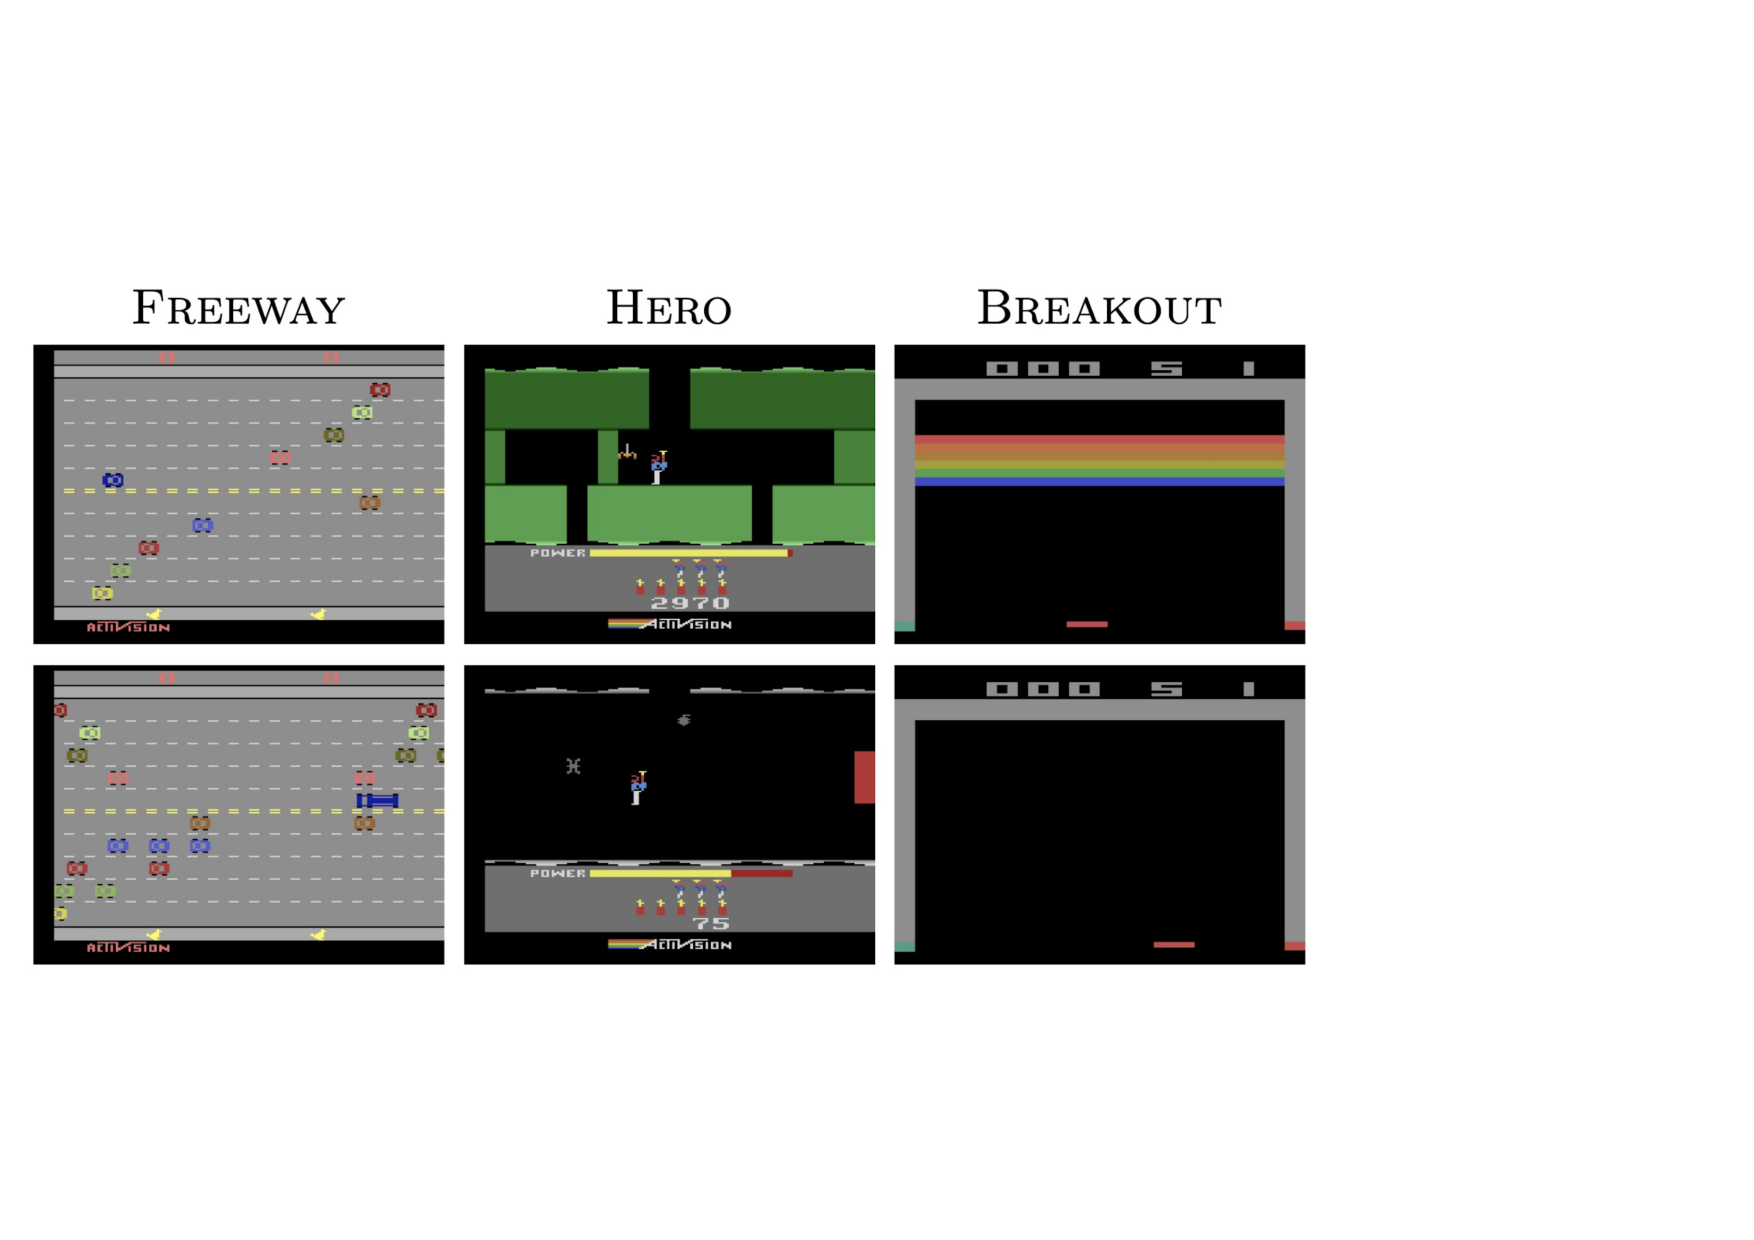
\includegraphics[width=0.35\linewidth]{chapters/scaled_ql/figures/atari_modes_3games.pdf}
        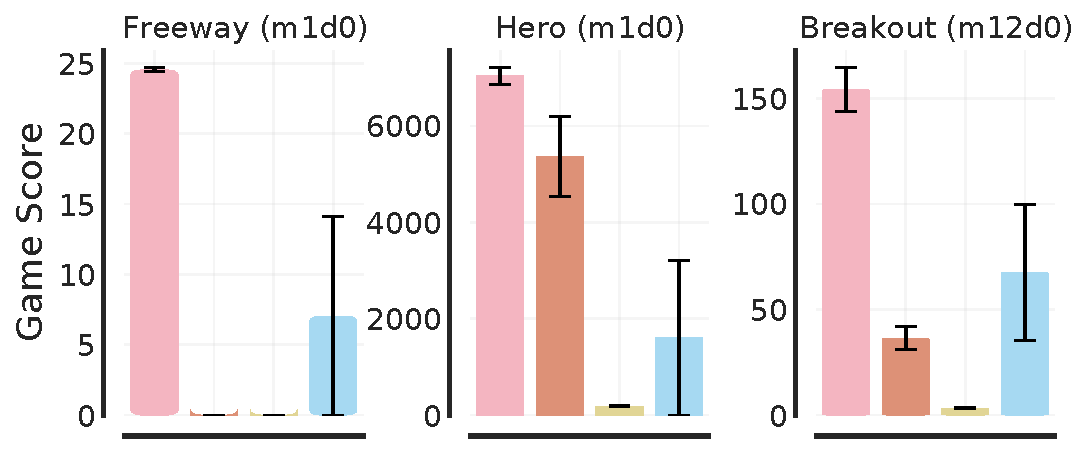
\includegraphics[width=0.5\linewidth]{chapters/scaled_ql/figures/online_ft_3_games.pdf}
    \vspace{-0.1cm}
    \caption{\footnotesize{\textbf{Online fine-tuning} results on unseen game \emph{variants}. \textbf{Left}. The top row shows default variants and the bottom row shows unseen variants evaluated for transfer: Freeway’s mode 1 adds buses, more vehicles, and increases velocity; Hero’s mode 1 starts the agent at level 5; Breakout’s mode 12 hides all bricks unless the ball has recently collided with a brick. \textbf{Right}. We fine-tune all methods except single-game DQN for 3M online frames (as we wish to test fast online adaptation). Error bars show minimum and maximum scores across 2 runs while the bar shows their average. Observe that scaled QL significantly outperforms learning from scratch and single-game DQN with 50M online frames. Furthermore, scaled QL also outperforms RL fine-tuning on representations learned using masked auto-encoders. See Figure~\ref{fig:lr_curves_online_ft} for learning curves.}}
    \label{fig:online_ft}
    \vspace{-0.5cm}
\end{figure}


\vspace{-0.25cm}
\subsubsection{Ablation Studies}
\label{sec:ablation}
\vspace{-0.25cm}

Finally, in this section we perform controlled ablation studies to understand how crucial the design decisions introduced in Section~\ref{sec:scaledql_method} are for the success of scaled Q-learning. In particular, we will attempt to understand the benefits of using C51 and feature normalization.

\textbf{MSE vs C51:} We ran scaled Q-learning with identical network architectures (ResNet 50 and ResNet 101), with both the conventional squared error formulation of TD error, and compare it to C51, which our main results utilize. Observe in Table~\ref{tab:ablation_mse} that C51 leads to much better performance for both ResNet 50 and ResNet 101 models. The boost in performance is the largest for ResNet 101, where C51 improves by over \textbf{39\%} as measured by median human-normalized score. This observation is surprising since prior work~\citep{agarwal2021deep} has shown that C51 performs on par with standard DQN with an Adam optimizer, which all of our results use. One hypothesis is that this could be the case as TD gradients would depend on the scale of the reward function, and hence some games would likely exhibit a stronger contribution in the gradient. This is despite the fact that our implementation of MSE TD-error already attempts to correct for this issue by applying the unitary scaling technique from \citep{kurin2022defense} to standardize reward scales across games. That said, we still observe that C51 performs significantly better.

\begin{table}[t]
    \centering
% \fontsize{8}{8}\selectfont
    \centering
    \vspace{-0.3cm}
    \caption{\footnotesize{\textbf{Performance of Scaled QL with the standard mean-squared TD-error and C51} in the offline 40-game setting aggregated by the median human-normalized score. Observe that for both ResNet 50 and ResNet 101, utilizing C51 leads to a drastic improvement in performance.}}% (as large as 39.4\% improvement on human-median normalized score with ResNet 101).}}
    \label{tab:ablation_mse}
    \vspace{0.1cm}
\resizebox{0.6\linewidth}{!}{\begin{tabular}{lcc}
\toprule
 & \textbf{Scaled QL (ResNet 50)} & \textbf{Scaled QL (ResNet 101)} \\
\midrule
\textbf{with MSE}  &  41.1\% & 59.5\%  \\
\midrule
\textbf{with C51}  & 53.5\% (+12.4\%) & 98.9\% (+39.4\%) \\
\bottomrule
\vspace{-0.25in}
\end{tabular}}
\end{table}


\textbf{Importance of feature normalization:} We ran small-scale experiments with and without feature normalization (Section~\ref{sec:scaledql_method}). In these experiments, we consider a multi-game setting with only 6 games: \textsc{Asterix}, \textsc{Breakout}, \textsc{Pong}, \textsc{SpaceInvaders}, \textsc{Seaquest}, and we train with the initial 20\% data for each game. We report aggregated median human-normalized score across the 6 games in Table~\ref{tab:ablation_dr3} for three different network architectures (ResNet 34, ResNet 50 and ResNet 101). Observe that the addition of feature normalization significantly improves performance for all the models. Motivated by this initial empirical finding, we used feature normalization in all of our main experiments. Overall, the above ablation studies validate the efficacy of the two key design decisions in this chapter. 
% However, there are several avenues for future investigation: 1) it is unclear if C51 works better because of the distributional formulation or the categorical representation and experiments with other distributional formulations could answer this question, 2) we did not extensively try alternate feature normalization schemes which may improve results. 

\begin{table}[ht]
    \centering
% \fontsize{8}{8}\selectfont
    \centering
    \vspace{-0.2cm}
    \caption{\footnotesize{\textbf{Performance of Scaled QL with and without feature normalization in the 6 game setting} reported in terms of the median human-normalized score. Observe that with models of all sizes, the addition of feature normalization improves performance.}}
    \label{tab:ablation_dr3}
    \vspace{0.1cm}
\resizebox{\linewidth}{!}{\begin{tabular}{lccc}
\toprule
 & \textbf{Scaled QL (ResNet 34)} & \textbf{Scaled QL (ResNet 50)} & \textbf{Scaled QL (ResNet 101)} \\
\midrule
\textbf{without feature normalization}  &  50.9\%  & 73.9\% & 80.4\%    \\
\midrule
\textbf{with feature normalization}  & 78.0\% (+28.9\%)  & 83.5\% (+9.6\%)  & 98.0\% (+17.6\%) \\
\bottomrule
\vspace{-0.2in}
\end{tabular}
}
\end{table}

\textbf{Additional ablations:} We also conducted ablation studies for the choice of the backbone architecture (spatial learned embeddings) in Appendix~\ref{app:backbone_ablation}, and observed that utilizing spatial embeddings is better. We also evaluated the performance of scaled QL without conservatism to test the importance of utilizing pessimism in our setting with diverse data in Appendix~\ref{app:no_pessimism}, and observe that pessimism is crucial for attaining good performance on an average. We also provide some scaling studies for another offline RL method (discrete BCQ) in Appendix~\ref{app:discrete_bcq}.


% \vspace{-0.2in}
% \section{Discussion}
% \vspace{-0.2in}
% \label{sec:discussion}
% \vspace{-3pt}
% Summary
\section{Discussion} 
We characterized the implicit preference of TD-learning towards solutions that maximally co-adapt gradients (or features) at consecutive state-action tuples that appear in Bellman backup. This regularization effect is exacerbated when out-of-sample
state-action samples are used for the Bellman backup and it can lead to poor policy performance. Inspired by the theory, we propose a practical explicit regularizer, \methodname, that yields substantial improvements in stability and performance on a wide range of offline RL problems. We believe that understanding the learning dynamics of deep Q-learning will lead to more robust and stable deep RL algorithms and enable predicting such instability issues, well in advance, which can inspire cross-validation and model selection strategies. This is an important, open challenge in offline RL, for which existing off-policy evaluation techniques are not practically sufficient~\citep{fu2021benchmarks}. 
% We also note that our analysis does not consider the online RL setting with non-stationary data distributions, and extending our theory and DR3 to online RL is an interesting avenue for future work.
% \textbf{Limitations:} 
% While DR3 improves performance on a number of tasks, it is not clear if it is the best possible approach to mitigate the issues we observe. Answering this question requires a deep understanding of the learning dynamics of Q-learning. 
% \textbf{Societal Impacts:} 
% Learning-based machine learning systems can have both positive (e.g., positive economic impact) and negative societal impacts  (e.g., loss of jobs in some areas). These implications also broadly apply to our work as any other work in reinforcement learning, and are largely not unique to this work.   

% % \newpage
% \section*{Reproducibility Statement}
% %% ICLR website --
% % https://iclr.cc/Conferences/2022/AuthorGuide
% % It is important that the work published in ICLR is reproducible. Authors are strongly encouraged to include a paragraph-long Reproducibility Statement at the end of the main text (before references) to discuss the efforts that have been made to ensure reproducibility. 

% %%SL.10.27: Generally, I'm in favor of deleting any conference specific junk from the arxiv version (it seems like conferences change their mind about what kind of statement or checklist they want every 3 months, so it kind of feels like nonsense like this won't stand the test of time)
% To ensure reproducibility in our empirical results, we provide complete experimental details regarding methods and hyper-parameters used in the Appendix~\ref{app:additional_background}. Additionally, we follow the recommendations of \citet{agarwal2021precipice} for reliable evaluation in deep RL and report the statistical uncertainty in reported results including aggregate performance metrics. We provide individual scores in Appendix~\ref{app:full_results} and we
% will release scores for individual runs as well as open-source our code. For theoretical results, we provide explanations of all the assumptions and a complete proof of the claims in Appendix~\ref{app:proofs}.

\section*{Acknowledgements}
We thank Dibya Ghosh, Xinyang Geng, Dale Schuurmans, Marc Bellemare, Pablo Castro and Ofir Nachum for informative discussions, discussions on experimental setup and for providing feedback on an early version of this paper. We thank the members of RAIL at UC Berkeley for their support and suggestions. We thank anonymous reviewers for feedback on an early version of this paper. This research is funded in part by the DARPA Assured Autonomy Program and in part, by compute resources from Microsoft Azure and Google Cloud. TM acknowledges support of Google Faculty Award, NSF IIS 2045685, the Sloan fellowship, and JD.com. 

\bibliography{reference}
\bibliographystyle{iclr2022_conference}

\appendix
\newpage
\section{Discussion of CQL Variants}
\label{app:cql_variants}
We derive several variants of CQL in Section~\ref{sec:framework}. Here, we discuss these variants on more detail and describe their specific properties. We first derive the variants: CQL($\mathcal{H}$), CQL($\rho$), and then present another variant of CQL, which we call CQL(var). This third variant has strong connections to distributionally robust optimization~\citep{namkoong2017variance}.

\textbf{CQL($\mathcal{H}$).} In order to derive CQL($\mathcal{H}$), we substitute $\mathcal{R} = \mathcal{H}(\mu)$, and solve the optimization over $\mu$ in closed form for a given Q-function. For an optimization problem of the form:
\begin{equation*}
    \max_{\mu}~~ \E_{\bx \sim \mu(\bx)}[f(\bx)] + \mathcal{H}(\mu)~~~ \text{s.t.}~~~ \sum_{\bx} \mu(\bx) = 1,~ \mu({\bx}) \geq 0~ \forall \bx,
\end{equation*}
the optimal solution is equal to $\mu^*(\bx) = \frac{1}{Z} \exp(f(\bx))$, where $Z$ is a normalizing factor. Plugging this into Equation~\ref{eqn:cql_framework}, we exactly obtain Equation~\ref{eqn:practical_objective}.

\textbf{CQL($\rho$).} In order to derive CQL($\rho$), we follow the above derivation, but our regularizer is a KL-divergence regularizer instead of entropy.
\begin{equation*}
    \small{\max_{\mu}~~ \E_{\bx \sim \mu(\bx)}[f(\bx)] + D_{\mathrm{KL}}(\mu || \rho)~~~ \text{s.t.}~~~ \sum_{\bx} \mu(\bx) = 1,~ \mu({\bx}) \geq 0~ \forall \bx}.
\end{equation*}
The optimal solution is given by, $\mu^*(\bx) = \frac{1}{Z} \rho(\bx) \exp(f(\bx))$, where $Z$ is a normalizing factor. Plugging this back into the CQL family (Equation~\ref{eqn:cql_framework}), we obtain the following objective for training the Q-function (modulo some normalization terms):
\begin{equation}
    \small{\min_{Q}~ \alpha \E_{\bs \sim d^\behavior(\bs)}\left[\E_{\mathbf{a} \sim \rho(\mathbf{a}|\bs)} \left[Q(\bs, \mathbf{a}) \frac{\exp(Q(\bs, \mathbf{a}))}{Z'}\right] - \E_{\mathbf{a} \sim \behavior(\mathbf{a}|\bs)}\left[Q(\bs, \mathbf{a})\right]\right] + \frac{1}{2}\!\E_{\bs, \mathbf{a}, \bs' \sim \mathcal{D}}\left[\left(Q - \bellman^{\policy_k} \hat{Q}^{k} \right)^2 \right]\!.}
    \label{eqn:cql_rho_objective}
\end{equation}

\textbf{CQL(var).} Finally, we derive a CQL variant that is inspired from the perspective of distributionally robust optimization (DRO)~\citep{namkoong2017variance}. This version penalizes the variance in the Q-function across actions at all states $\bs$, under some action-conditional distribution of our choice. In order to derive a canonical form of this variant, we invoke an identity from \citet{namkoong2017variance}, which helps us simplify Equation~\ref{eqn:cql_framework}. To start, we define the notion of ``robust expectation'': for any function $f(\bx)$, and any empirical distribution $\hat{P}(\bx)$ over a dataset $\{ \bx_1, \cdots, \bx_N\}$ of $N$ elements, the ``robust'' expectation defined by: 
\begin{equation*}
    R_N(\hat{P}) := \max_{\mu(\bx)} ~~\E_{\bx \sim \mu(\bx)}[f(\bx)] \text{~~~s.t.~~~} D_{f}(\mu(\bx), \hat{P}(\bx)) \leq \frac{\delta}{N},
\end{equation*}    
can be approximated using the following upper-bound:
\begin{equation}
    R_N(\hat{P}) \leq \E_{\bx \sim \hat{P}(\bx)}[f(\bx)] + \sqrt{\frac{2 \delta~ \text{var}_{\hat{P}(\bx)}(f(\bx))}{N}},
    \label{eqn:robust_expectation}
\end{equation}
where the gap between the two sides of the inequality decays inversely w.r.t. to the dataset size, $\mathcal{O}(1/N)$. By using Equation~\ref{eqn:robust_expectation} to simplify Equation~\ref{eqn:cql_framework}, we obtain an objective for training the Q-function that penalizes the variance of Q-function predictions under the distribution $\hat{P}$. 
\begin{multline}
    \min_{Q}~~ \frac{1}{2}~ \E_{\bs, \mathbf{a}, \bs' \sim \mathcal{D}}\left[\left(Q - \bellman^{\policy_k} \hat{Q}^{k} \right)^2 \right] + \alpha \E_{\bs \sim d^\behavior(\bs)}\left[\sqrt{\frac{\text{var}_{\hat{P}(\mathbf{a}|\bs)}\left( Q(\bs, \mathbf{a}) \right)}{d^\behavior(s) |\mathcal{D}|}} \right] \\ 
    + \alpha \E_{s \sim d^\behavior(\bs)}\left[ \E_{\hat{P}(\mathbf{a}|\bs)}[Q(\bs, \mathbf{a})] - \E_{\behavior(\mathbf{a}|\bs)}[Q(\bs, \mathbf{a})] \right]
    \label{eqn:variance_regularized_again}
\end{multline}
The only remaining decision is the choice of $\hat{P}$, which can be chosen to be the inverse of the empirical action distribution in the dataset, $\hat{P}(\mathbf{a}|\bs) \propto \frac{1}{\hat{D}(\mathbf{a}|\bs)}$, or even uniform over actions, $\hat{P}(\mathbf{a}|\bs) = \text{Unif}(\mathbf{a})$, to obtain this variant of variance-regularized CQL.

% \textbf{CQL with variable state distributions.} The formulations of CQL in Sections~\ref{sec:policy_eval} and \ref{sec:framework} only use a variable action distribution $\mu(\mathbf{a}|\bs)$. In principle, we can extend these formulations to account for a variable state-distribution as well. In order to do this, we can modify Equation~\ref{eqn:objective_1} as follows:
% \begin{multline}
%     \label{eqn:cql_framework_state_dist}
%     \small{\min_{Q} ~~ \alpha \E_{\bs \sim \textcolor{red}{\mu(\bs)}, \mathbf{a} \sim \textcolor{red}{\mu(\mathbf{a}|\bs)}}\left[Q(\bs, \mathbf{a})\right] + \frac{1}{2}~ \E_{\bs, \mathbf{a}, \bs' \sim \mathcal{D}}\left[\left(Q(\bs, \mathbf{a}) - \bellman^{\policy} \hat{Q}^{k} (\bs, \mathbf{a}) \right)^2 \right].}
% \end{multline}
% In this case, the resulting tabular Q-function iterate, $\hat{Q}^k$ is given by:
% \begin{equation*}
% \hat{Q}^{k+1}(\bs, \mathbf{a}) = \bellman^\policy \hat{Q}^k (\bs, \mathbf{a}) - \alpha \left[\frac{\mu(\bs) \mu(\mathbf{a}|\bs)}{d^\behavior(\bs) \behavior(\mathbf{a}|\bs)} - 1\right].
% \end{equation*}
% We note that analogous to Proposition~\ref{thm:cql_underestimates}, we can argue that this is a lower bound estimate, since a positive quantity (i.e. density ratios) is being subtracted from the ideal tabular Q-function backup, at each iteration.

\section{Discussion of Gap-Expanding Behavior of CQL Backups}
\label{app:gap_amplify}
\vspace{-0.25cm}
% now lets talk about the section that compares prior methods and CQL with function approximation in terms of action gap
%%SL.5.11: I wonder if it could make sense to have a single "Related Work and Connections to Policy Constraints" section, where we could have a subsection on "Related Prior Work" subsection on "Prior Work on Offline RL with Constraints" and "Comparative Analysis of CQL and Policy Constraint Methods" or something? Not certain about this, but maybe we try it and see how it looks? It's a bit unconventional...

% setup the stage, what we want to do in this section and why
In this section, we discuss in detail the consequences of the gap-expanding behavior of CQL backups over prior methods based on policy constraints that, as we show in this section, may not exhibit such gap-expanding behavior in practice. To recap, Theorem~\ref{thm:gap_amplify} shows that the CQL backup operator increases the difference between expected Q-value at in-distribution ($\ba \sim \behavior(\ba|\bs)$) and out-of-distribution ($\ba \text{~s.t.~} \frac{\mu_k(\ba|\bs)}{\behavior(\ba|\bs)} << 1$) actions. We refer to this property as the gap-expanding property of the CQL update operator.

% This gap-expanding behavior plays a central role when learning in the presence of function approximation:  

% In this section, we perform an analysis of CQL with deep neural networks, and compare it to prior offline RL methods based on policy constraints. As noted in Section~\ref{sec:related}, some variants of CQL can be viewed as applying a policy constraint on the greedy policy induced by the Q-function. We therefore aim to analyze the effect of direct regularization on the Q-function as opposed to only constraining the policy, with primary focus on settings where function approximation is employed.

% discuss why policy constraint methods may fail
\textbf{Function approximation may give rise to erroneous Q-values at OOD actions.} We start by discussing the behavior of prior methods based on policy constraints~\citep{kumar2019stabilizing,fujimoto2018off,jaques2019way,wu2019behavior} in the presence of function approximation.
To recap, because computing the target value requires $\E_\policy[\hat{Q}(\bs,\ba)]$, constraining $\policy$ to be close to $\behavior$ will avoid evaluating $\hat{Q}$ on OOD actions. These methods typically do not impose any further form of regularization on the learned Q-function.
Even with policy constraints, because function approximation used to represent the Q-function, learned Q-values at two distinct state-action pairs are coupled together. As prior work has argued and shown~\citep{achiam2019towards,fu2019diagnosing,kumar2020discor}, the ``generalization'' or the coupling effects of the function approximator may be heavily influenced by the properties of the data distribution~\citep{fu2019diagnosing,kumar2020discor}. For instance, \citet{fu2019diagnosing} empirically shows that when the dataset distribution is narrow (i.e. state-action marginal entropy, $\mathcal{H}(d^\behavior(\bs, \ba))$, is low~\citep{fu2019diagnosing}), the coupling effects of the Q-function approximator can give rise to incorrect Q-values at different states, though this behavior is absent without function approximation, and is not as severe with high-entropy (e.g. Uniform) state-action marginal distributions.
%%SL.5.27: The above sentence is really speculative -- I don't think it's at all clear why narrow datasets couple different state action pairs. It's also very hard to understand, because it's long, with multiple clauses, and nested parentheses. I would really recommend just deleting the whole sentence. But if you don't want to delete it, try to rewrite to more clearly explain the point, with shorter sentences, avoiding complex clauses, and avoiding parens whenever possible.
% done, cited prior work diagnosing bottlenecks and DisCor

In offline RL, we will shortly present empirical evidence on high-dimensional MuJoCo tasks showing that certain dataset distributions, $\mathcal{D}$, may cause the learned Q-value at an OOD action $\ba$ at a state $\bs$, to in fact take on high values than Q-values at in-distribution actions at intermediate iterations of learning. This problem persists even when a large number of samples (e.g. $1M$) are provided for training, and the agent cannot correct these errors due to no active data collection.  

%%AK.5.29: Toned down to one para, with mostly pointing to the analysis, not creating any hypotheses for why something might be going wrong.
Since actor-critic methods, including those with policy constraints, use the learned Q-function to train the policy, in an iterative online policy evaluation and policy improvement cycle, as discussed in Section~\ref{sec:background}, the errneous Q-function may push the policy towards OOD actions, especially when no policy constraints are used. Of course, policy constraints should prevent the policy from choosing OOD actions, however, as we will show that in certain cases, policy constraint methods might also fail to prevent the effects on the policy due to incorrectly high Q-values at OOD actions. 

% how do these Q-values affect the policy?
% \textbf{How can erroneous Q-values affect the quality of the resulting policy?} When these erroneous Q-values -- with higher relative values
% at out-of-distribution actions -- are used to then update the policy, the policy is pushed towards OOD actions, since a policy improvement update, shown below, trains the policy to maximize Q-values:
% \begin{equation}
%     \label{eqn:policy_constraint_repeated}
%     \policy^{k+1}~~ \leftarrow \arg \max_{\textcolor{red}{\policy}} \E_{\bs \sim d^\behavior(\bs)}\left[ \E_{\ba \sim \textcolor{red}{\policy}}[\hat{Q}^{k+1}(\bs, \ba)] - \nu_k \underbrace{D(\textcolor{red}{\policy}(\ba|\bs), \behavior(\ba|\bs))}_{\text{policy constraint}} \right]
% \end{equation}
% % Of course, when policy constraints are used, the policy is prevented from choosing OOD actions. 
% % However, a gradient signal obtained from such an erroneous Q-function will still push the policy towards OOD actions, since the Q-values at these OOD actions are relatively higher than in-distribution actions. We discuss empirical evidence justifying this in Appendix~\ref{app:empirical_evidence_gap_expanding}. 
% %%SL.5.27: A reviewer might say this should not be an issue, since you won't get OOD actions due to the constraint
% % We have empirical evidence for this, that atleast in some cases this could be an issue, but the example, and the experiments, I feel should justify this in practice
% However, the low fidelity of the Q-function combined with the inability to correct errors in the function this case, may just push the policy towards OOD actions, directly conflicting with the policy-constraint. While this might not be potentially harmful when the Q-function provides enough improvement signal to improve the policy when the policy constraint is satisfied, but this property may not be guaranteed. 

% As a result, the improvement signal obtained from the Q-function might directly conflicts with the policy constraint, whose role is to prevent the policy from choosing OOD actions. We would instead desire that the Q-function provides enough improvement signal to the policy within the space of in-distribution actions, so that the policy can improve within the set of observed actions. But since Q-values may be higher at OOD actions, the Q-function gradient may push the policy towards OOD actions as a result, and hence directly conflict with the policy constraint (which aims at keeping the policy within in a close neighbourhood of the behavior cloned policy).  
% When gradient based optimization is used to train the policy in this setting, this could amount to conflicting gradient (as we show via empirical evidence), and hence, it is likely that the overall update shown in Equation~\ref{eqn:policy_constraint_repeated} does not improve the policy meaningfully. 
%%SL.5.27: this seems very vague and imprecise, and it's not clear how CQL does this
% restated below

\textbf{How can CQL address this problem?} As we show in Theorem~\ref{thm:gap_amplify}, the difference between expected Q-values at in-distribution actions and out-of-distribution actions is expanded by the CQL update. This property is a direct consequence of the specific nature of the CQL regularizer -- that maximizes Q-values under the dataset distribution, and minimizes them otherwise. This difference depends upon the choice of $\alpha_k$, which can directly be controlled, since it is a free parameter. Thus, by effectively controlling $\alpha_k$, CQL can push down the learned Q-value at out-of-distribution actions as much is desired, correcting for the erroneous overestimation error in the process.  


%%SL.5.27: Overall, I really don't find the discussion above to be very convincing. It seems very speculative, and it's very easy to argue with and disagree with. Are you sure we can't somehow delete the stuff above, and instead present this appendix as a summary of the evidence that we'll be discussing below? I also think we should really consider simply deleting this appendix. It was a nice idea, but the quality of the evidence here is really not up to the standard of rigor, and perhaps it's better to omit it than to include things that are too debatable or too hand-wavy. Basically, I have a hard time imagining how this appendix will make anyone happy -- anyone who is skeptical about our method will become even more skeptical, whereas anyone who likely our method will probably not read this appendix (because it's not about our method).

% why is this problem more relevant in offline settings?
% We also remark that while the problem induced due to Q-function approximation also afflicts standard online Q-function training (and this is a motivation behind gap-increasing operators~\citep{bellemare2016increasing}), we would expect this problem to more severely affect performance in offline RL. Q-function errors in standard online RL can be corrected in most cases~\citep{kumar2020discor,levine2020offline}, since the agent can collect new transitions that correspond to highly erroneous Q-values and then train on them. However, the algorithm cannot perform any online data collection and moreover, has no control over the dataset, $\mathcal{D}$ either in offline RL settings, making the impact of this problem severe. We next present a simple didactic example to demonstrate this problem.

% example
% \subsection{Didactic Example} 
% \label{app:didactic_example}
% In order to build intuition for the discussion presented above, we consider a didactic three-state, two-action MDP shown in Figure~\ref{fig:didactic}. Action $\ba_1$ at state $\bs_0$ deterministically transits to state $\bs_2$, and action $\ba_2$ at state $\bs_0$ transits to state $\bs_1$. Both actions at state $\bs_1$ and $\bs_2$ induce a self-loop at $\bs_1$ and $\bs_2$ respectively. The MDP provides the following reward values: $r(\bs_0, \ba_1) = 10, r(\bs_1, \ba_2) = -5$ and all other rewards, $r(\bs_1, \cdot) = 0, r(\bs_2, \cdot) = 0$. Assume that the offline dataset at state $\bs_0$ is distributed according to the following density function: $\mathcal{D}(\ba_1|\bs_0) = 0.8, \mathcal{D}(\ba_2|\bs_0) = 0.2$, and also assume that the size of the dataset $\mathcal{D}$ is so large, that the dataset empirical densities match the actual distribution of the behavior policy, i.e., $\mathcal{D}(\bs, \ba) = d^\behavior(\bs, \ba)$. The Q-function is modeled as a linear 
% \begin{wrapfigure}{r}{0.35\textwidth}
% \vspace{-10pt}
% \begin{center}
% \begin{tikzpicture}[auto,node distance=8mm,>=latex,font=\small]
%     \tikzstyle{round}=[thick,draw=black,circle]

%     \node[round] (s0) {$\bs_0$};
%     \node[round,above right=0mm and 20mm of s0] (s1) {$\bs_1$};
%     \node[round,below right=0mm and 20mm of s0] (s2) {$\bs_2$};

%     \draw[->] (s0) -- (s1) node[midway,sloped,above] {$\ba_2, -5$};
%     \draw[->] (s0) -- (s2) node[midway,sloped,below] {$\ba_1, +10$};
% \end{tikzpicture}
% \end{center}
% \caption{\small{Didactic three-state, two-action example demonstrating how the generalization effects of the Q-function approximator can hurt policy learning in offline RL, even with a (support-based) policy constraint.}}
% \vspace{-25pt}
% \label{fig:didactic}
% \end{wrapfigure}
% function on a scalar-valued given feature $\phi(\bs, \ba)$, such that $\hat{Q}(\bs, \ba) = w \cdot \phi(\bs, \ba) + b$. Assume $\phi(\bs_0, \ba_1) = 1$ and $\phi(\bs_0, \ba_2) = 1 + \varepsilon$, for some $\varepsilon > 0$, $\phi(\bs_1, \ba_1) = \phi(\bs_1, \ba_2) = 1 + \delta$, and $\phi(\bs_2, \ba_1) = \phi(\bs_2, \ba_2) = 0$. 

% %%AK: read this para and make more concrete
% When a policy-constraint that constrains the policy to the support of the behavior policy is used to update the Q-function, the updated Q-function parameters satisfy: $w_1 > 0$ and $b_1 > 0$. This is because an action with a high reward is used to minimize the Bellman error, and this pushes the Q-function to output positive values. Observe that the Q-function corresponding to these new-parameters also satisfies, $\hat{Q}^{1}(\bs_0, \ba_2) > \hat{Q}^{1}(\bs_0, \ba_1)$, which erroneously makes action $\ba_2$ have a higher Q-value. Since both actions are in the support of the behavior policy at state $\bs_0$, the incorrect Q-function updates the policy towards selecting action $\ba_2$ at state $\bs_0$, which gives rise to a negative reward. On the other hand, if the overestimation in the value $\hat{Q}(\bs_0, \ba_2)$ is controlled, as is the case with CQL (since, $\ba_2$ has a lower density under the behavior policy, and CQL would expand the gap, $\hat{Q}(\bs_0, \ba_1) - \hat{Q})(\bs_0, \ba_2)$, then we obtain $w^1 < 0$ and $b^1 >0$, thus preventing this issue. 

\textbf{Empirical evidence on high-dimensional benchmarks with neural networks.}  
We next empirically demonstrate the existence of of such Q-function estimation error on high-dimensional MuJoCo domains when deep neural network function approximators are used with stochastic optimization techniques. In order to measure this error, we plot the difference in expected Q-value under actions sampled from the behavior distribution, $\ba \sim \behavior(\ba|\bs)$, and the maximum Q-value over actions sampled from a uniformly random policy, $\ba \sim \text{Unif}(\ba|\bs)$. That is, we plot the quantity
\begin{equation}
\label{eqn:delta_eqn}
    \hat{\Delta}^k = \E_{\bs, \ba \sim \mathcal{D}}\left[\max_{\ba'_1, \cdots, \ba'_N \sim \text{Unif}(\ba')}[\hat{Q}^k(\bs, \ba')]- \hat{Q}^k(\bs, \ba)\right]
\end{equation}
over the iterations of training, indexed by $k$. This quantity, intuitively, represents an estimate of the ``advantage'' of an action $\ba$, under the Q-function, with respect to the optimal action $\max_{\ba'} \hat{Q}^k(\bs, \ba')$. Since, we cannot perform exact maximization over the learned Q-function in a continuous action space to compute $\Delta$, we estimate it via sampling described in Equation~\ref{eqn:delta_eqn}.

We present these plots in Figure~\ref{fig:delta_plots} on two datasets: hopper-expert and hopper-medium. The expert dataset is generated from a near-deterministic, expert policy, exhibits a narrow coverage of the state-action space, and limited to only a few directed trajectories. On this dataset, we find that $\hat{\Delta}^k$ is always positive for the policy constraint method (Figure~\ref{fig:delta_plots}(a)) and increases during training -- note, the continuous rise in $\hat{\Delta}^k$ values, in the case of the policy-constraint method, shown in Figure~\ref{fig:delta_plots}(a). This means that even if the dataset is generated from an expert policy, and policy constraints correct target values for OOD actions,
%%SL.5.27: Maybe it's because this sentence has too many clauses, but I don't actually understand what "near-optimal policy and policy constraints are used" means
% edited
incorrect Q-function generalization may make an out-of-distribution action appear promising. For the more stochastic hopper-medium dataset, that consists of a more diverse set of trajectories, shown in Figure~\ref{fig:delta_plots}(b), we still observe that $\hat{\Delta}^k > 0$ for the policy-constraint method, however, the relative magnitude is smaller than hopper-expert.

In contrast, Q-functions learned by CQL, generally satisfy $\hat{\Delta}^k < 0$, as is seen  and these values are clearly smaller than those for the policy-constraint method. This provides some empirical evidence for Theorem~\ref{thm:gap_amplify}, in that, the maximum Q-value at a randomly chosen action from the uniform distribution the action space is smaller than the Q-value at in-distribution actions.

On the hopper-expert task, as we show in Figure~\ref{fig:delta_plots}(a) (right), we eventually observe an ``unlearning'' effect, in the policy-constraint method where the policy performance deteriorates after a extra iterations in training. This ``unlearning'' effect is similar to what has been observed when standard off-policy Q-learning algorithms without any policy constraint are used in the offline regime~\citep{kumar2019stabilizing,levine2020offline}, on the other hand this effect is absent in the case of CQL, even after equally many training steps. The performance in the more-stochastic hopper-medium dataset fluctuates, but does not deteriorate.
%%AK.5.30: need some ending.. what do these plots suggest.

To summarize this discussion, we concretely observed the following points via empirical evidence:
\begin{itemize}
\vspace{-10pt}
    \item CQL backups are gap expanding in practice, as justified by the negative $\hat{\Delta}^k$ values in Figure~\ref{fig:delta_plots}.
    \item Policy constraint methods, that do not impose any regularization on the Q-function may observe highly positive $\hat{\Delta}^k$ values during training, especially with narrow data distributions, indicating that gap-expansion may  be absent.
    \item When $\hat{\Delta}^k$ values continuously grow during training, the policy might eventually suffer from an unlearning effect~\citep{levine2020offline}, as shown in Figure~\ref{fig:delta_plots}(a).
    \vspace{-10pt}
\end{itemize}

\begin{figure}
    \begin{subfigure}[h]{0.49\linewidth}
      \centering
      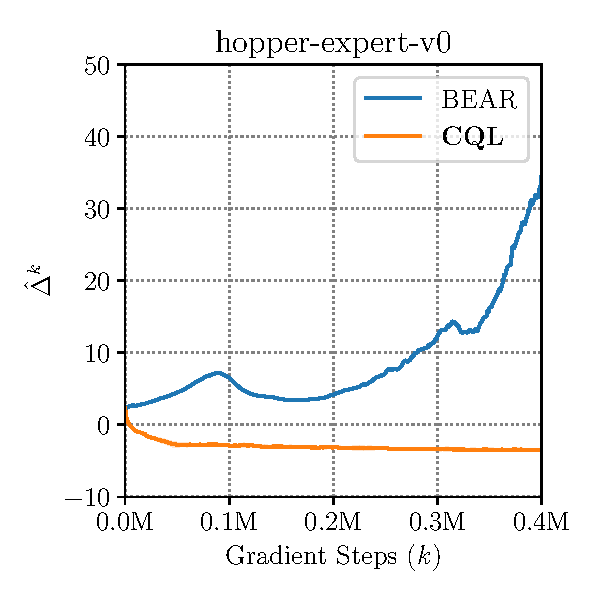
\includegraphics[width=0.47\linewidth]{NeuRIPS2019/images/hopper-expert-v0bear_vs_cql.pdf}
      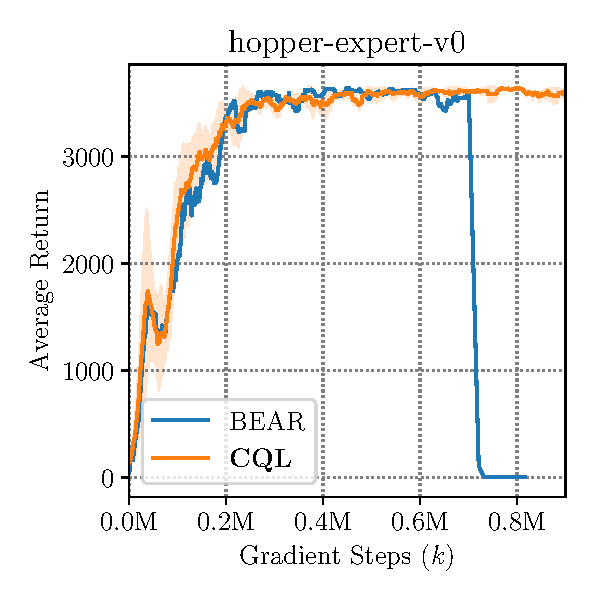
\includegraphics[width=0.47\linewidth]{NeuRIPS2019/images/hopper-expert-v0bear_vs_cql_return.pdf}
      \caption{hopper-expert-v0}
    \end{subfigure}
    ~
    \begin{subfigure}[h]{0.49\linewidth}
      \centering
      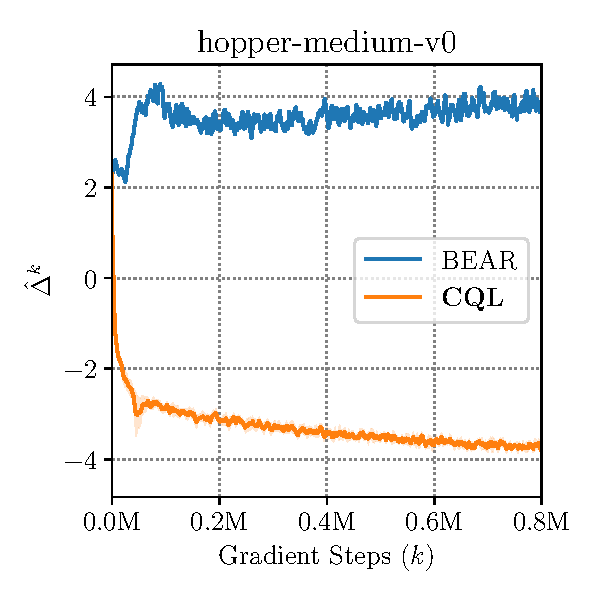
\includegraphics[width=0.47\linewidth]{NeuRIPS2019/images/hopper-medium-v0bear_vs_cql_again.pdf}
      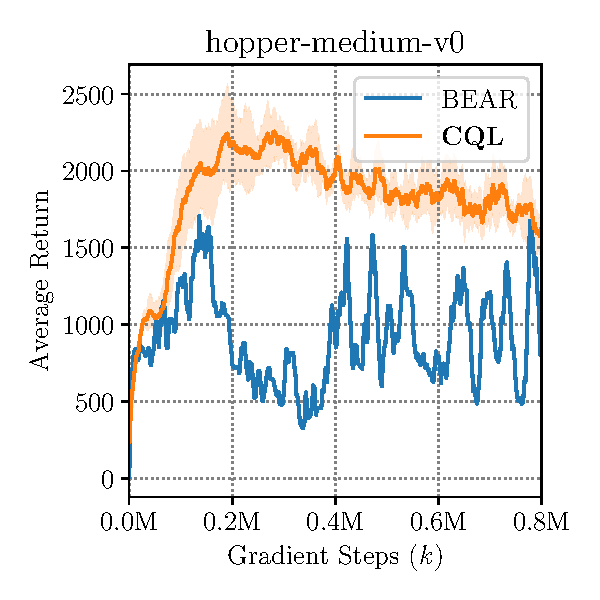
\includegraphics[width=0.47\linewidth]{NeuRIPS2019/images/hopper-medium-v0bear_vs_cql_again_return.pdf}
      \caption{hopper-medium-v0}
      %%SL.5.27: label the plots -- label both axes and title
    \end{subfigure}
    \caption{$\Delta^k$ as a function of training iterations for hopper-expert and hopper-medium datasets. Note that CQL (left) generally has negative values of $\Delta$, whereas BEAR (right) generally has positive $\Delta$ values, which also increase during training with increasing $k$ values.}
    %%SL.5.27: Make sure caption at least briefly summarizes the implications of this
    \label{fig:delta_plots}
\end{figure}

% \textbf{Why does CQL solve this problem?} Theorem~\ref{thm:gap_amplify} indicates that, by appropriately controlling for $\alpha_k$, CQL can ensure that the learned $\hat{\Delta}^k$ is larger than the actual value of $\Delta^k$ in the MDP (when evaluated using the true Q-function, $Q^k$). That is, for all $k$, we have that $\hat{\Delta}^k > \Delta^k$ under appropriate choices of $\alpha_1, \cdots, \alpha_k$. Empirically, this translates to generally negative (or positive with a small magnitude) values of $\hat{\Delta}^k$ for CQL, as shown in Figure~\ref{fig:delta_plots}(a) and (b). Note that it is sufficient for the empirical $\hat{\Delta}^k$ to be larger than $\Delta^k$, and not necessarily negative. 
% %%AK.5.26: Revisit this statement once.
% CQL generally maintains a negative value of $\hat{\Delta}^k$, and this difference is reflected in better and more stable final policy performance for CQL, as shown in Figure ??, even without a policy constraint. 


\vspace{-0.3cm}
\section{Theorem Proofs}
\label{app:missing_proofs}
\vspace{-0.3cm}

In this section, we provide proofs of the theorems in Sections~\ref{sec:policy_eval} and \ref{sec:framework}. We first redefine notation for clarity and then provide the proofs of the results in the main paper.

\textbf{Notation.} Let $k \in \mathbb{N}$ denote an iteration of policy evaluation (in Section~\ref{sec:policy_eval}) or Q-iteration (in Section~\ref{sec:framework}). In an iteration $k$, the objective -- Equation~\ref{eqn:modified_policy_eval} or Equation~\ref{eqn:cql_framework} -- is optimized using the previous iterate (i.e. $\hat{Q}^{k-1}$) as the target value in the backup. $Q^k$ denotes the true, tabular Q-function iterate in the MDP, without any correction. In an iteration, say $k+1$, the current tabular Q-function iterate, $Q^{k+1}$ is related to the previous tabular Q-function iterate ${Q}^k$ as: $Q^{k+1} = \bellman^{\policy} Q^k$ (for policy evaluation) or $Q^{k+1} = \bellman^{\policy_k} Q^k$ (for policy learning). Let $\hat{Q}^k$ denote the $k$-th Q-function iterate obtained from CQL. Let $\hat{V}^k$ denote the value function, $\hat{V}^k := \E_{\mathbf{a} \sim \policy(\mathbf{a}|\bs)}[\hat{Q}^k(\bs, \mathbf{a})]$.   

\textbf{A note on the value of $\alpha$.} Before proving the theorems, we remark that while the statements of Theorems~\ref{thm:cql_underestimates}, \ref{thm:min_q_underestimates} and \ref{thm:policy_eval_func_approx} (we discuss this in Appendix~\ref{app:additional_theory}) show that CQL produces lower bounds if $\alpha$ is larger than some threshold, so as to overcome either sampling error (Theorems~\ref{thm:cql_underestimates} and \ref{thm:min_q_underestimates}) or function approximation error (Theorem~\ref{thm:policy_eval_func_approx}). While the optimal $\alpha_k$ in some of these cases depends on the current Q-value, $\hat{Q}^k$, we can always choose a worst-case value of $\alpha_k$ by using the inequality $\hat{Q}^k \leq 2 R_{\max}/(1 - \gamma)$, still guaranteeing a lower bound. If it is unclear why the learned Q-function $\hat{Q}^k$ should be bounded, we can always clamp the Q-values if they go outside $\left[ \frac{-2 R_{\max}}{1 - \gamma}, \frac{2 R_{\max}}{1 - \gamma} \right]$.
We first prove Theorem~\ref{thm:min_q_underestimates}, which shows that policy evaluation using a simplified version of CQL (Equation~\ref{eqn:objective_1}) results in a point-wise lower-bound on the Q-function. 

~

\niparagraph{\large{Proof of Theorem~\ref{thm:min_q_underestimates}}} 


We start by analyzing $\hat{Q}^k$ by setting the derivative of Equation~\ref{eqn:objective_1} to 0:
\begin{equation}
    \forall~\bs, \mathbf{a} \in \mathcal{D}, k, ~~ \hat{Q}^{k+1}(\bs, \mathbf{a}) = \hat{\bellman}^\pi \hat{Q}^k(\bs, \mathbf{a}) - \alpha \frac{\mu(\mathbf{a}|\bs)}{\hatbehavior(\mathbf{a}|\bs)}.
    \label{eqn:q_expression_objective1}
\end{equation}
Now, since, $\mu(\mathbf{a}|\bs) > 0, \alpha > 0, \hatbehavior(\mathbf{a}|\bs) > 0$, we observe that at each iteration we underestimate the next Q-value iterate, i.e. $\hat{Q}^{k+1} \leq \hat{\bellman}^\policy \hat{Q}^k$.

\textbf{Accounting for sampling error.} Note that so far we have only shown that the Q-values are upper-bounded by the the ``empirical Bellman targets'' given by, $\hat{\bellman}^\policy \hat{Q}^k$. In order to relate $\hat{Q}^k$ to the true Q-value iterate, $Q^k$, we need to relate the empirical Bellman operator, $\hat{\bellman}^\policy$ to the actual Bellman operator, $\bellman^\policy$. In Appendix~\ref{app:handling_unobserved_actions}, we show that if the reward function $r(\bs, \mathbf{a})$ and the transition function, $\transitions(\bs'|\bs, \mathbf{a})$ satisfy ``concentration'' properties, meaning that the difference between the observed reward sample, $r$ ($\bs, \mathbf{a}, r, \bs') \in \mathcal{D}$) and the actual reward function $r(\bs, \mathbf{a})$ (and analogously for the transition matrix) is bounded with high probability, then overestimation due to the empirical Backup operator is bounded. Formally, with high probability (w.h.p.) $\geq 1 - \delta$, $\delta \in (0, 1)$, 
\begin{equation*}
    \forall Q, \bs, \mathbf{a} \in \mathcal{D},~~ \left\vert \hat{\bellman}^\policy Q(\bs, \mathbf{a}) - \bellman^\policy Q(\bs, \mathbf{a}) \right\vert \leq \frac{C_{r, T, \delta} R_{\max}}{(1 - \gamma) \sqrt{|\mathcal{D}(\bs, \mathbf{a})|}}.
\end{equation*}
Hence, the following can be obtained, w.h.p.:
\begin{align}
\label{eqn:pac_bound_q_value}
    \hat{Q}^{k+1}(\bs, \mathbf{a}) = \bellman^\policy \hat{Q}^k(\bs, \mathbf{a}) \leq \bellman^\policy \hat{Q}^k(\bs, \mathbf{a}) - \alpha \frac{\mu(\mathbf{a}|\bs)}{\hatbehavior(\mathbf{a}|\bs)} + \frac{C_{r, T, \delta} R_{\max}}{(1 - \gamma) \sqrt{|\mathcal{D}(\bs, \mathbf{a})|}}.
\end{align}

Now we need to reason about the fixed point of the update procedure in Equation~\ref{eqn:q_expression_objective1}. The fixed point of Equation~\ref{eqn:q_expression_objective1} is given by:
\begin{multline*}
    \hat{Q}^\policy \leq \bellman^\policy \hat{Q}^\policy - \alpha \frac{\mu(\mathbf{a}|\bs)}{\hatbehavior(\mathbf{a}|\bs)} + \frac{C_{r, T, \delta} R_{\max}}{(1 - \gamma) \sqrt{|\mathcal{D}(\bs, \mathbf{a})|}} \implies \hat{Q}^\pi \leq (I - \gamma P^\pi)^{-1} \left[ R  - \alpha \frac{\mu}{\hatbehavior} + \frac{C_{r, T, \delta} R_{\max}}{1 - \gamma) \sqrt{|\mathcal{D}}}\right]\\
    \hat{Q}^\policy(\bs, \mathbf{a}) \leq Q^\policy(\bs, \mathbf{a}) - \alpha \left[ \left(I - \gamma P^\pi \right)^{-1} \left[\frac{\mu}{\hatbehavior} \right] \right](\bs, \mathbf{a}) + \left[(I - \gamma P^\policy)^{-1} \frac{C_{r, T, \delta} R_{\max}}{(1 - \gamma) \sqrt{|\mathcal{D}|}} \right](\bs, \mathbf{a}),
\end{multline*}
thus proving the relationship in Theorem~\ref{thm:min_q_underestimates}.

In order to guarantee a lower bound, $\alpha$ can be chosen to cancel any potential overestimation incurred by $\frac{C_{r, T, \delta} R_{\max}}{(1 - \gamma)\sqrt{|\mathcal{D}|}}$. Note that this  choice works, since $(I - \gamma P^\pi)^{-1}$ is a matrix with all non-negative entries. The choice of $\alpha$ that guarantees a lower bound is then given by:
\begin{align*}
    \alpha& ~ \cdot \min_{\bs, \mathbf{a}} \left[\frac{\mu(\mathbf{a}|\bs)}{\hatbehavior(\mathbf{a}|\bs)} \right] \geq \max_{\bs, \mathbf{a}} \frac{C_{r, T, \delta} R_{\max}}{(1 - \gamma) \sqrt{|\mathcal{D}(\bs, \mathbf{a})|}}\\
    \implies \alpha&~ \geq \max_{\bs, \mathbf{a}} \frac{C_{r, T, \delta} R_{\max}}{(1 - \gamma) \sqrt{|\mathcal{D}(\bs, \mathbf{a})|}} \cdot \max_{\bs, \mathbf{a}} \left[\frac{\mu(\mathbf{a}|\bs)}{\hatbehavior(\mathbf{a}|\bs)} \right]^{-1}.
\end{align*}
Note that the theoretically minimum possible value of $\alpha$ decreases as more samples are observed, i.e., when $|\mathcal{D}(\bs, \mathbf{a})|$ is large. Also, note that since, $\frac{C_{r, T, \delta} R_{\max}}{(1 - \gamma0 \sqrt{|\mathcal{D}|}} \approx 0$, when $\hat{\bellman}^\policy = \bellman^\policy$, any $\alpha \geq 0$ guarantees a lower bound. And so choosing a value of $\alpha = 0$ is sufficient in this case.

Next, we prove Theorem~\ref{thm:cql_underestimation} that shows that the additional term that maximizes the expected Q-value under the dataset distribution, $\mathbb{D}(\bs, \mathbf{a})$, (or $d^\behavior(\bs) \behavior(\mathbf{a}|\bs)$, in the absence of sampling error), results in a lower-bound on only the expected value of the policy at a state, and not a pointwise lower-bound on Q-values at all actions.

~

\niparagraph{\large{Proof of Theorem~\ref{thm:cql_underestimates}}} 


We first prove this theorem in the absence of sampling error, and then incorporate sampling error at the end, using a technique similar to the previous proof. In the tabular setting, we can set the derivative of the modified objective in Equation~\ref{eqn:modified_policy_eval}, and compute the Q-function update induced in the exact, tabular setting (this assumes $\hat{\bellman}^\policy = \bellman^\policy)$ and $\behavior(\mathbf{a}|\bs) = \hatbehavior(\mathbf{a}|\bs)$).
\begin{equation}
    \forall ~\bs, \mathbf{a}, k ~~ \hat{Q}^{k+1} (\bs, \mathbf{a}) = \bellman^\policy \hat{Q}^k(\bs, \mathbf{a}) - \alpha \left[\frac{\mu(\mathbf{a}|\bs)}{\behavior(\mathbf{a}|\bs)} - 1 \right].
    \label{eqn:q_function_modified_eval}
\end{equation}
Note that for state-action pairs, $(\bs, \mathbf{a})$, such that, $\mu(\mathbf{a}|\bs) < \behavior(\mathbf{a}|\bs)$, we are infact adding a positive quantity, $1 - \frac{\mu(\mathbf{a}|\bs)}{\behavior(\mathbf{a}|\bs)}$, to the Q-function obtained, and this we cannot guarantee a point-wise lower bound, i.e. $\exists~ \bs, \mathbf{a}, \text{~~s.t.}~~ \hat{Q}^{k+1}(\bs, \mathbf{a}) \geq Q^{k+1}(\bs, \mathbf{a})$. To formally prove this, we can construct a counter-example three-state, two-action MDP, and choose a specific behavior policy $\policy(\mathbf{a}|\bs)$, such that this is indeed the case.

The value of the policy, on the other hand, $\hat{V}^{k+1}$ is underestimated, since:
\begin{equation}
    \hat{V}^{k+1}(\bs) := \E_{\mathbf{a} \sim \policy(\mathbf{a}|\bs)} \left[ \hat{Q}^{k+1}(\bs, \mathbf{a}) \right] = \bellman^\policy \hat{V}^k (\bs) - \alpha \E_{\mathbf{a} \sim \policy(\mathbf{a}|\bs)}\left[\frac{\mu(\mathbf{a}|\bs)}{\behavior(\mathbf{a}|\bs)} - 1 \right].
    \label{eqn:value_recursion}
\end{equation}
and we can show that $D_{\text{CQL}}(\bs): = \sum_{\mathbf{a}} \policy(\mathbf{a}|\bs) \left[\frac{\mu(\mathbf{a}|\bs)}{\behavior(\mathbf{a}|\bs)} - 1 \right]$ is always positive, when $\policy(\mathbf{a}|\bs) = \mu(\mathbf{a}|\bs)$. To note this, we present the following derivation:
\begin{align*}
    D_{\text{CQL}}(\bs) &:=~ \sum_{\mathbf{a}} \policy(\mathbf{a}|\bs) \left[\frac{\mu(\mathbf{a}|\bs)}{\behavior(\mathbf{a}|\bs)} - 1 \right]\\
    &= \sum_{\mathbf{a}} (\policy(\mathbf{a}|\bs) - \behavior(\mathbf{a}|\bs) + \behavior(\mathbf{a}|\bs)) \left[\frac{\mu(\mathbf{a}|\bs)}{\behavior(\mathbf{a}|\bs)} - 1 \right]\\
    &= \sum_{\mathbf{a}} (\policy(\mathbf{a}|\bs) - \behavior(\mathbf{a}|\bs)) \left[ \frac{\policy(\mathbf{a}|\bs) - \behavior(\mathbf{a}|\bs)}{\behavior(\mathbf{a}|\bs} \right] + \sum_{\mathbf{a}} \behavior(\mathbf{a}|\bs) \left[\frac{\mu(\mathbf{a}|\bs)}{\behavior(\mathbf{a}|\bs)} - 1 \right]\\
    &= \sum_{\mathbf{a}} \underbrace{\left[ \frac{\left(\policy(\mathbf{a}|\bs) - \behavior(\mathbf{a}|\bs) \right)^2}{\behavior(\mathbf{a}|\bs)} \right]}_{\geq 0}~ +~ 0 \text{~~~since,~} \sum_{\mathbf{a}} \policy(\mathbf{a}|\bs) = \sum_{\mathbf{a}} \behavior(\mathbf{a}|\bs) = 1.
\end{align*}
Note that the marked term, is positive since both the numerator and denominator are positive, and this implies that $D_\text{CQL}(\bs) \geq 0$. Also, note that $D_\text{CQL}(\bs) = 0$, iff $\policy(\mathbf{a}|\bs) = \behavior(\mathbf{a}|\bs)$. This implies that each value iterate incurs some underestimation, $\hat{V}^{k+1}(\bs) \leq \bellman^\policy \hat{V}^k (\bs)$.

Now, we can compute the fixed point of the recursion in Equation~\ref{eqn:value_recursion}, and this gives us the following estimated policy value:
\begin{equation*}
    \hat{V}^\policy(\bs) = V^\policy(\bs) - \alpha \left[ \underbrace{(I - \gamma P^\policy)^{-1}}_{\text{non-negative entries}}
    \underbrace{\E_{\policy}\left[\frac{\policy}{\behavior} - 1 \right]}_{\geq 0} \right](\bs),
\end{equation*}
thus showing that in the absence of sampling error, Theorem~\ref{thm:cql_underestimates} gives a lower bound. It is straightforward to note that this expression is tighter than the expression for policy value in Proposition~\ref{thm:cql_underestimates}, since, we explicitly subtract $1$ in the expression of Q-values from the previous proof.

\textbf{Incorporating sampling error.} To extend this result to the setting with sampling error, similar to the previous result, the maximal overestimation at each iteration $k$, is bounded by $\frac{C_{r, T, \delta} R_{\max}}{1 - \gamma}$.
The resulting value-function satisfies (w.h.p.), $\forall \bs \in \mathcal{D}$, 
\begin{equation*}
   \hat{V}^\policy(\bs) \leq V^\policy(\bs) - \alpha \left[\left(I - \gamma P^\pi \right)^{-1} \E_{\policy}\left[\frac{\policy}{\hatbehavior} - 1 \right] \right](\bs) + \left[ (I - \gamma P^\pi)^{-1} \frac{C_{r, T, \delta} R_{\max}}{(1- \gamma) \sqrt{|\mathcal{D}|}}\right](\bs)
\end{equation*}
thus proving the theorem statement. In this case, the choice of $\alpha$, that prevents overestimation w.h.p. is given by:
\begin{equation*}
    \alpha \geq \max_{\bs, \mathbf{a} \in \mathcal{D}} \frac{C_{r, T} R_{\max}}{(1 - \gamma) \sqrt{|\mathcal{D}(\bs, \mathbf{a})|}} \cdot \max_{\bs \in \mathcal{D}} \left[\sum_{\mathbf{a}} \policy(\mathbf{a}|\bs) \left(\frac{\policy(\mathbf{a}|\bs)}{\hatbehavior(\mathbf{a}|\bs))} - 1\right)\right]^{-1}.
\end{equation*}
Similar to Theorem~\ref{thm:min_q_underestimates}, note that the theoretically acceptable value of $\alpha$ decays as the number of occurrences of a state action pair in the dataset increases.
Next we provide a proof for Theorem~\ref{thm:cql_underestimation}.

~

\niparagraph{\large{Proof of Theorem~\ref{thm:cql_underestimation}}} 

In order to prove this theorem, we compute the difference induced in the policy value, $\hat{V}^{k+1}$, derived from the Q-value iterate, $\hat{Q}^{k+1}$, with respect to the previous iterate $\bellman^\policy \hat{Q}^{k}$. If this difference is negative at each iteration, then the resulting Q-values are guaranteed to lower bound the true policy value.

\begin{align*}
    \E_{\hat{\policy}^{k+1}(\mathbf{a}|\bs)}[\hat{Q}^{k+1}(\bs, \mathbf{a})] &=  \E_{\hat{\policy}^{k+1}(\mathbf{a}|\bs)}\left[ \bellman^\policy \hat{Q}^k (\bs, \mathbf{a}) \right] - \E_{\hat{\policy}^{k+1}(\mathbf{a}|\bs)}\left[ \frac{\pi_{\hat{Q}^k}(\mathbf{a} | \bs)}{\hatbehavior(\mathbf{a}|\bs)} -1 \right]\\
    &= \E_{\hat{\policy}^{k+1}(\mathbf{a}|\bs)}\left[ \bellman^\policy \hat{Q}^k (\bs, \mathbf{a}) \right] - \underbrace{\E_{\policy_{\hat{Q}^k}(\mathbf{a} | \bs)}\left[ \frac{\policy_{\hat{Q}^k}(\mathbf{a} | \bs)}{\hatbehavior(\mathbf{a}|\bs)} -1 \right]}_{\text{underestimation, ~~(a)}}\\
    &~~~~~~~~~~~~~~~~~~~~~~~~~~~~~+ \sum_{\mathbf{a}} \underbrace{\left(\policy_{\hat{Q}^k}(\mathbf{a} | \bs) - \hat{\policy}^{k+1}(\mathbf{a}|\bs) \right)}_{\text{(b),}~~{\leq \mathrm{D_{TV}}(\policy_{\hat{Q}^k}, \hat{\policy}^{k+1})}} \frac{\policy_{\hat{Q}^k}(\mathbf{a} | \bs)}{\hatbehavior(\mathbf{a}|\bs)}
    %   \E_{\pi_{\hat{Q}^k}(\mathbf{a} | \bs)}[\hat{Q}^{k+1}(\bs, \mathbf{a})] - 
\end{align*}
If (a) has a larger magnitude than (b), then the learned Q-value induces an underestimation in an iteration $k+1$, and hence, by a recursive argument, the learned Q-value underestimates the optimal Q-value. We note that by upper bounding term (b) by $\mathrm{D_{TV}}(\policy_{\hat{Q}^k}, \hat{\policy}^{k+1}) \cdot \max_{\mathbf{a}} \frac{\policy_{\hat{Q}^k}(\mathbf{a} | \bs)}{\hatbehavior(\mathbf{a}|\bs)}$, and writing out (a) > upper-bound on (b), we obtain the desired result.


Finally, we show that under specific choices of $\alpha_1, \cdots, \alpha_k$, the CQL backup is gap-expanding by providing a proof for Theorem~\ref{thm:gap_amplify}.

~

\niparagraph{\large{Proof of Theorem~\ref{thm:gap_amplify} (CQL is gap-expanding)}}

For this theorem, we again first present the proof in the absence of sampling error, and then incorporate sampling error into the choice of $\alpha$. We follow the strategy of observing the Q-value update in one iteration. Recall that the expression for the Q-value iterate at iteration $k$ is given by:
\begin{equation*}
    \hat{Q}^{k+1}(\bs, \mathbf{a}) = \bellman^{\policy^k} \hat{Q}^{k}(\bs, \mathbf{a}) - \alpha_k \frac{\mu_k(\mathbf{a}|\bs) - \behavior(\mathbf{a}|\bs)}{\behavior(\mathbf{a}|\bs)}.
\end{equation*}
Now, the value of the policy $\mu_{k}(\mathbf{a}|\bs)$ under $\hat{Q}^{k+1}$ is given by:
\begin{equation*}
    \E_{\mathbf{a} \sim \mu_k(\mathbf{a}|\bs)}[\hat{Q}^{k+1}(\bs, \mathbf{a})] = \E_{\mathbf{a} \sim \mu_k(\mathbf{a}|\bs)}[\bellman^{\policy^k} \hat{Q}^k (\bs, \mathbf{a})] - \alpha_k \underbrace{\mu_k^T \left(\frac{\mu_k(\mathbf{a}|\bs) - \behavior(\mathbf{a}|\bs)}{\behavior(\mathbf{a}|\bs)} \right)}_{:= \hat{\Delta}^k, \geq 0, \text{~~by proof of Theorem~\ref{thm:cql_underestimates}.}} 
\end{equation*}
Now, we also note that the expected amount of extra underestimation introduced at iteration $k$ under action sampled from the behavior policy $\behavior(\mathbf{a}|\bs)$ is 0, as,
\begin{equation*}
    \E_{\mathbf{a} \sim \behavior(\mathbf{a}|\bs)}[\hat{Q}^{k+1}(\bs, \mathbf{a})] = \E_{\mathbf{a} \sim \behavior(\mathbf{a}|\bs)}[\bellman^{\policy^k} \hat{Q}^k (\bs, \mathbf{a})] - \alpha_k \underbrace{\behavior^T \left(\frac{\mu_k(\mathbf{a}|\bs) - \behavior(\mathbf{a}|\bs)}{\behavior(\mathbf{a}|\bs)} \right)}_{= 0}. 
\end{equation*}
where the marked quantity is equal to 0 since it is equal since $\behavior(\mathbf{a}|\bs)$ in the numerator cancels with the denominator, and the remaining quantity is a sum of difference between two density functions, $\sum_{\mathbf{a}} \mu_k(\mathbf{a}|\bs) - \behavior(\mathbf{a}|\bs)$, which is equal to 0. Thus, we have shown that,
\begin{equation*}
    \E_{\behavior(\mathbf{a}|\bs)}[\hat{Q}^{k+1}(\bs, \mathbf{a})] - \E_{\mu_k(\mathbf{a}|\bs)}[\hat{Q}^{k+1}(\bs, \mathbf{a})] = \E_{\behavior(\mathbf{a}|\bs)}[\bellman^{\policy^k} \hat{Q}^k (\bs, \mathbf{a})] - \E_{\mu_k(\mathbf{a}|\bs)}[\bellman^{\policy^k} \hat{Q}^k (\bs, \mathbf{a})] - \alpha_k \hat{\Delta}^k.
\end{equation*}
Now subtracting the difference, $\E_{\behavior(\mathbf{a}|\bs)}[Q^{k+1}(\bs, \mathbf{a})] - \E_{\mu_k(\mathbf{a}|\bs)}[Q^{k+1}(\bs, \mathbf{a})]$, computed under the tabular Q-function iterate, $Q^{k+1}$, from the previous equation, we obtain that
\begin{multline*}
    \E_{\mathbf{a} \sim \behavior(\mathbf{a}|\bs)}[\hat{Q}^{k+1}(\bs, \mathbf{a})] - \E_{\behavior(\mathbf{a}|\bs)}[{Q}^{k+1}(\bs, \mathbf{a})] = \E_{\mu_k(\mathbf{a}|\bs)}[\hat{Q}^{k+1}(\bs, \mathbf{a})] - \E_{\mu_k(\mathbf{a}|\bs)}[{Q}^{k+1}(\bs, \mathbf{a})]\\
    + (\mu_k(\mathbf{a}|\bs) - \behavior(\mathbf{a}|\bs))^T \underbrace{\left[ \bellman^{\policy^k} \left( \hat{Q}^k - Q^k \right)(\bs, \cdot) \right]}_{(a)}- \alpha_k \hat{\Delta}^k.
\end{multline*}
% Now, by invoking Theorem~\ref{thm:cql_underestimation}, we note that the quantity marked as (a) in the previous equation is negative, since it is the expected difference between $\hat{Q}^k - \hat{Q}^k$ under the policy iterate, $\policy^k$. 

Now, by choosing $\alpha_k$, such that any positive bias introduced by the quantity $(\mu_k(\mathbf{a}|\bs) - \behavior(\mathbf{a}|\bs))^T (a)$ is cancelled out, we obtain the following gap-expanding relationship:
\begin{equation*}
    \E_{\mathbf{a} \sim \behavior(\mathbf{a}|\bs)}[\hat{Q}^{k+1}(\bs, \mathbf{a})] - \E_{\behavior(\mathbf{a}|\bs)}[{Q}^{k+1}(\bs, \mathbf{a})] > \E_{\mu_k(\mathbf{a}|\bs)}[\hat{Q}^{k+1}(\bs, \mathbf{a})] - \E_{\mu_k(\mathbf{a}|\bs)}[{Q}^{k+1}(\bs, \mathbf{a})]
\end{equation*}
for, $\alpha_k$ satisfying, 
\begin{equation*}
    \alpha_k > \max \left(\frac{(\behavior(\mathbf{a}|\bs) - \mu_k(\mathbf{a}|\bs))^T \left[ \bellman^{\policy^k} \left( \hat{Q}^k - Q^k \right)(\bs, \cdot) \right]}{\hat{\Delta}^k}, 0\right),
\end{equation*}
thus proving the desired result.

To avoid the dependency on the true Q-value iterate, ${Q}^k$, we can upper-bound $Q^k$ by $\frac{R_{\max}}{1 - \gamma}$, and upper-bound $(\behavior(\mathbf{a}|\bs) - \mu_k(\mathbf{a}|\bs))^T \bellman^{\policy^k} Q^k (\bs, \cdot)$ by $D_{\mathrm{TV}}(\behavior, \mu_k) \cdot \frac{R_{\max}}{1 - \gamma}$, and use this in the expression for $\alpha_k$. While this bound may be loose, it still guarantees the gap-expanding property, and we indeed empirically show the existence of this property in practice in Appendix~\ref{app:gap_amplify}. 

To incorporate sampling error, we can follow a similar strategy as previous proofs: the worst case overestimation due to sampling error is given by $\frac{C_{r, T, \delta} R_{\max}}{1 - \gamma}$. In this case, we note that, w.h.p.,
\begin{equation*}
    \left\vert \hat{\bellman}^{\policy^k} \left( \hat{Q}^k - Q^k \right) - \bellman^{\policy^k} \left( \hat{Q}^k - Q^k \right) \right\vert \leq \frac{2 \cdot C_{r, T, \delta} R_{\max}}{1 - \gamma}. 
\end{equation*}
Hence, the presence of sampling error adds $D_{\mathrm{TV}}(\hat{\behavior}, \mu_k) \cdot \frac{2 \cdot C_{r, T, \delta} R_{\max}}{1 - \gamma}$ to the value of $\alpha_k$, giving rise to the following, sufficient condition on $\alpha_k$ for the gap-expanding property:
\begin{equation*}
     \alpha_k > \max \left(\frac{(\behavior(\mathbf{a}|\bs) - \mu_k(\mathbf{a}|\bs))^T \left[ \bellman^{\policy^k} \left( \hat{Q}^k - Q^k \right)(\bs, \cdot) \right]}{\hat{\Delta}^k} + D_{\mathrm{TV}}(\hat{\behavior}, \mu_k) \cdot \frac{2 \cdot C_{r, T, \delta} R_{\max}}{1 - \gamma}, 0\right),
\end{equation*}
concluding the proof of this theorem.

% \vspace{-0.1cm}
\section{Additional Theoretical Analysis}
\label{app:additional_theory}
% \vspace{-0.2cm}

In this section, we present a theoretical analysis of additional properties of CQL. For ease of presentation, we state and prove theorems in Appendices~\ref{app:cql_linear_non_linear} and \ref{app:maximizing_distributions} in the absence of sampling error, but as discussed extensively in Appendix~\ref{app:missing_proofs}, we can extend each of these results by adding extra terms induced due to sampling error. 

\subsection{CQL with Linear and Non-Linear Function Approximation}
\label{app:cql_linear_non_linear}
\begin{theorem}
\label{thm:policy_eval_func_approx}
Assume that the Q-function is represented as a linear function of given state-action feature vectors $\Qfeat$, i.e., $Q(s, a) = w^T \Qfeat(s, a)$. Let $D = \text{diag}\left(d^\behavior(\bs) \behavior(\mathbf{a}|\bs)\right)$ denote the diagonal matrix with data density, and assume that $\Qfeat^T D \Qfeat$ is invertible. Then, the expected value of the policy under Q-value from Eqn~\ref{eqn:modified_policy_eval} at iteration $k+1$, $\E_{d^\behavior(\mathbf{a})}[\hat{V}^{k+1}(\bs)] = \E_{d^\behavior(\bs), \policy(\mathbf{a}|\bs)}[\hat{Q}^{k+1}(\bs, \mathbf{a})]$, lower-bounds the corresponding tabular value, $\E_{d^\behavior(\bs)}[V^{k+1}(\bs)] =\E_{d^\behavior(\bs), \policy(\mathbf{a}|\bs)}[Q^{k+1}(\bs, \mathbf{a})]$, if
\begin{equation*}
\small{\alpha_k \geq \max \left(\frac{D^T\left[\Qfeat \left(\Qfeat^T D \Qfeat \right)^{-1} \Qfeat^T - I \right]\left((\bellman^\policy \hat{Q}^k)(\bs, \mathbf{a})\right)}{D^T\left[ \Qfeat \left(\Qfeat^T D \Qfeat \right)^{-1} \Qfeat^T \right] \left(D \left[\frac{\policy(\mathbf{a}|\bs) - \behavior(\mathbf{a}|\bs)}{\behavior(\mathbf{a}|\bs)} \right] \right)},~ 0 \right).}
    %  \small{\alpha_k \geq \max \left(\frac{\left(d^\behavior(\bs) \mu(\mathbf{a}|\bs)\right)^T\left[\Qfeat \left(\Qfeat^T D \Qfeat \right)^{-1} \Qfeat^T - I \right]\left((\bellman^\policy \hat{Q}^k)(\bs, \mathbf{a})\right)}{\left(d^\behavior(\bs) \mu(\mathbf{a}|\bs)\right)^T\left[ \Qfeat \left(\Qfeat^T D \Qfeat \right)^{-1} \Qfeat^T \right] \left(d^\behavior(\bs) \left( \mu(\mathbf{a}|\bs) - \behavior(\mathbf{a}|\bs) \right) \right)},~ 0 \right).}
\end{equation*}
\end{theorem}
%intuitive justification for the theorem
The choice of $\alpha_k$ in Theorem~\ref{thm:policy_eval_func_approx} intuitively amounts to compensating for overestimation in value induced if the true value function cannot be represented in the chosen linear function class (numerator), by the potential decrease in value due to the CQL regularizer (denominator). This implies that if the actual value function can be represented in the linear function class, such that the numerator can be made $0$, then \textbf{any} $\alpha > 0$ is sufficient to obtain a lower bound. We now prove the theorem.

\begin{proof} 
In order to extend the result of Theorem~\ref{thm:cql_underestimates} to account for function approximation, we follow the similar recipe as before. We obtain the optimal solution to the optimization problem below in the family of linearly expressible Q-functions, i.e. $\mathcal{Q} := \{\Qfeat w | w \in \mathbb{R}^{dim(\Qfeat)} \}$. 
\begin{equation*}
    \min_{Q \in \mathcal{Q}}~~ \alpha_k \cdot \left(\E_{d^\behavior(\bs),\mu(\mathbf{a}|\bs)}\left[Q(\bs, \mathbf{a})\right] - {\E_{d^\behavior(\bs),\behavior(\mathbf{a}|\bs)}\left[Q(\bs, \mathbf{a})\right]} \right) + \frac{1}{2}~ \E_{\mathcal{D}}\left[\left(Q(\bs, \mathbf{a}) - \bellman^\policy \hat{Q}^{k} (\bs, \mathbf{a}) \right)^2 \right].
\end{equation*}
By substituting $Q(\bs, \mathbf{a}) = w^T \Qfeat(\bs, \mathbf{a})$, and setting the derivative with respect to $w$ to be 0, we obtain,
\begin{align*}
    \alpha \sum_{\bs, \mathbf{a}} d^\behavior(\bs) \cdot \left( \mu(\mathbf{a}|\bs) - \behavior(\mathbf{a}|\bs) \right) \Qfeat(\bs, \mathbf{a}) + \sum_{\bs, \mathbf{a}} d^\behavior(\bs) \behavior(\mathbf{a}|\bs) \left( Q(\bs, \mathbf{a}) - \bellman^\pi \hat{Q}^k(\bs, \mathbf{a}) \right) \Qfeat(\bs, \mathbf{a}) = 0.
\end{align*}
By re-arranging terms, and converting it to vector notation, defining $D = \text{diag}(d^\behavior(\bs)\behavior(\bs))$, and referring to the parameter $w$ at the k-iteration as $w^k$ we obtain:
\begin{align*}
    \left(\Qfeat^T D \Qfeat \right) w^{k+1} = \underbrace{\Qfeat^T D \left( \bellman^\policy \hat{Q}^k \right)}_{\text{LSTD iterate}} - \underbrace{\alpha_k \Qfeat^T \text{diag}\left[d^\behavior(\bs) \cdot(\mu(\mathbf{a}|\bs) - \behavior(\mathbf{a}|\bs)) \right]}_{\text{underestimation}}.
\end{align*}
Now, our task is to show that the term labelled as ``underestimation'' is indeed negative in expectation under $\mu(\mathbf{a}|\bs)$ (This is analogous to our result in the tabular setting that shows underestimated values). In order to show this, we write out the expression for the value, under the linear weights $w^{k+1}$ at state $\bs$, after substituting $\mu = \policy$,
\begin{align}
    \hat{V}^{k+1}(\bs) &:= \policy(\mathbf{a}|\bs)^T \Qfeat w^{k+1}\\
    = \policy(&\mathbf{a}|\bs)^T \underbrace{\Qfeat \left(\Qfeat^T D \Qfeat \right)^{-1} \Qfeat^T D \left(\bellman^\policy \hat{Q}^k \right)}_{\text{value under LSTD-Q~\citep{lagoudakis2003least}}} - \alpha_k \policy(\mathbf{a}|\bs)^T \Qfeat \left(\Qfeat^T D \Qfeat \right)^{-1} \Qfeat^T D \left[\frac{\policy(\mathbf{a}|\bs) - \behavior(\mathbf{a}|\bs)}{\behavior(\mathbf{a}|\bs)} \right].
    \label{expr:lstdq_value}
\end{align}
Now, we need to reason about this additional penalty term. Defining, $P_\Qfeat := \Qfeat \left(\Qfeat^T D \Qfeat \right)^{-1} \Qfeat^T D$ as the projection matrix onto the subspace of features $\Qfeat$, we need to show that the product that appears as a penalty is positive: $\policy(\mathbf{a}|\bs)^T P_\Qfeat \left[\frac{\policy(\mathbf{a}|\bs) - \behavior(\mathbf{a}|\bs)}{\behavior(\mathbf{a}|\bs)} \right] \geq 0$. In order to show this, we compute minimum value of this product optimizing over $\policy$. If the minimum value is $0$, then we are done.

Let's define $f(\policy) = \policy(\mathbf{a}|\bs)^T P_\Qfeat \left[\frac{\policy(\mathbf{a}|\bs) - \behavior(\mathbf{a}|\bs)}{\behavior(\mathbf{a}|\bs)} \right]$, our goal is to solve for $\min_{\policy} f(\policy)$. Setting the derivative of $f(\policy)$ with respect to $\policy$ to be equal to 0, we obtain (including Lagrange multiplier $\eta$ that guarantees $\sum_{\mathbf{a}} \policy(\mathbf{a}|\bs) = 1$,
\begin{equation*}
    \left( P_\Qfeat + P_\Qfeat^T \right) \left[\frac{\policy(\mathbf{a}|\bs)}{\behavior(\mathbf{a}|\bs)}\right] = P_\Qfeat \Vec{1} + \eta \Vec{1}.
\end{equation*}
By solving for $\eta$ (using the condition that a density function sums to 1), we obtain that the minimum value of $f(\policy)$ occurs at a $\policy^*(\mathbf{a}|\bs)$, which satisfies the following condition,
\begin{equation*}
    \left(P_\Qfeat + P_\Qfeat^T \right) \left[\frac{\policy^*(\mathbf{a}|\bs)}{\behavior(\mathbf{a}|\bs)}\right] = \left( P_\Qfeat + P_\Qfeat^T \right) \Vec{1}.
\end{equation*}
Using this relation to compute $f$, we obtain, $f(\policy^*) = 0$, indicating that the minimum value of $0$ occurs when the projected density ratio matches under the matrix $(P_\Qfeat + P_\Qfeat^T)$ is equal to the projection of a vector of ones, $\Vec{1}$. Thus, \begin{equation*}
    \forall~ \policy(\mathbf{a}|\bs),~ f(\policy) = \policy(\mathbf{a}|\bs)^T P_{\Qfeat} \left[\frac{\policy(\mathbf{a}|\bs) - \behavior(\mathbf{a}|\bs)}{\behavior(\mathbf{a}|\bs)} \right] \geq 0.
\end{equation*}

This means that: $\forall ~\bs, \hat{V}^{k+1}(\bs) \leq \hat{V}^{k+1}_{\text{LSTD-Q}}(\bs)$ given identical previous $\hat{Q}^{k}$ values. This result indicates, that if $\alpha_k \geq 0$, the resulting CQL value estimate with linear function approximation is guaranteed to lower-bound the value estimate obtained from a least-squares temporal difference Q-learning algorithm (which only minimizes Bellman error assuming a linear Q-function parameterization), such as LSTD-Q~\citep{lagoudakis2003least}, since at each iteration, CQL induces a lower-bound with respect to the previous value iterate, whereas this underestimation is absent in LSTD-Q. Also note that we can also apply an inductive argument.

So far, we have only shown that the learned value iterate, $\hat{V}^{k+1}(\bs)$ lower-bounds the value iterate obtained from LSTD-Q, $\forall ~\bs, \hat{V}^{k+1}(\bs) \leq \hat{V}^{k+1}_{\text{LSTD-Q}}(\bs)$. But, our final aim is to prove a stronger result, that the learned value iterate, $\hat{V}^{k+1}$, lower bounds the exact tabular value function iterate, ${V}^{k+1}$, at each iteration. The reason why our current result does not guarantee this is because function approximation may induce overestimation error in the linear approximation of the Q-function.

In order to account for this change, we make a simple change: we choose $\alpha_k$ such that the resulting penalty nullifes the effect of any over-estimation caused due to the inability to fit the true value function iterate in the linear function class parameterized by $\Qfeat$. Formally, this means:
\begin{align*}
    \E_{d^\behavior(\bs)}\left[\hat{V}^{k+1}(\bs)\right] &\leq \E_{d^\behavior(\bs)}\left[\hat{V}^{k+1}_{\text{LSTD-Q}}(\bs)\right] - \alpha_k \E_{d^\behavior(\bs)}[f(\policy(\mathbf{a}|\bs))] \\
    & \leq \E_{d^\behavior(\bs)}\left[V^{k+1}(\bs)\right] - \underbrace{\E_{d^\behavior(\bs)}\left[\hat{V}^{k+1}_{\text{LSTD-Q}}(\bs) - V^{k+1}(\bs) \right] - \alpha_k \E_{d^\behavior(\bs)}[f(\policy(\mathbf{a}|\bs))]}_{\text{choose~} \alpha_k \text{~to make this negative}} \\
    & \leq \E_{d^\behavior(\bs)}\left[V^{k+1}(\bs)\right]
\end{align*}
And the choice of $\alpha_k$ in that case is given by:
\begin{align*}
    \alpha_k \geq& ~ \max \left(\frac{\E_{d^\behavior(\bs)}\left[\hat{V}^{k+1}_{\text{LSTD-Q}}(\bs) - V^{k+1}(\bs) \right]}{\E_{d^\behavior(\bs)}[f(\policy(\mathbf{a}|\bs))]}, 0 \right)\\
    \geq& ~ \max \left(\frac{D^T\left[\Qfeat \left(\Qfeat^T D \Qfeat \right)^{-1} \Qfeat^T - I \right]\left((\bellman^\policy \hat{Q}^k)(\bs, \mathbf{a})\right)}{D^T\left[ \Qfeat \left(\Qfeat^T D \Qfeat \right)^{-1} \Qfeat^T \right] \left(D \left[\frac{\policy(\mathbf{a}|\bs) - \behavior(\mathbf{a}|\bs)}{\behavior(\mathbf{a}|\bs)} \right] \right)},~ 0 \right).
\end{align*}
Finally, we note that since this choice of $\alpha_k$ induces under-estimation in the next iterate, $\hat{V}^{k+1}$ with respect to the previous iterate, $\hat{V}^k$, for all $k \in \mathbb{N}$, by induction, we can claim that this choice of $\alpha_1, \cdots, \alpha_k$ is sufficient to make $\hat{V}^{k+1}$ lower-bound the tabular, exact value-function iterate. $V^{k+1}$, for all $k$, thus completing our proof.
\end{proof}
% done

We can generalize Theorem~\ref{thm:policy_eval_func_approx} to non-linear function approximation, such as neural networks, {under the standard NTK framework~\citep{ntk}}, assuming that each iteration $k$ is performed by a single step of gradient descent on Equation~\ref{eqn:modified_policy_eval}, rather than a complete minimization of this objective. As we show in Theorem~\ref{corr:nonlinear_ntk}, CQL learns lower bounds in this case for an appropriate choice of $\alpha_k$. 
% We will also empirically show in Appendix~\ref{app:cql_additional_results} that CQL can learn effective conservative Q-functions with multilayer neural networks.

%%SL.5.30: I don't think this should be called a corollary. Corollaries are supposed to quick and easy to prove, if it takes the better part of a page to prove, it's not a corollary.
\begin{theorem}[Extension to non-linear function approximation]
\label{corr:nonlinear_ntk}
Assume that the Q-function is represented by a general non-linear function approximator parameterized by $\theta$, $Q_\theta(\bs, \mathbf{a})$. let $D = \text{diag}(d^\behavior(\bs) \behavior(\mathbf{a}|\bs))$ denote the matrix with the data density on the diagonal, and assume that $\nabla_\theta Q_\theta^T D \nabla_\theta Q_\theta$ is invertible. Then, the expected value of the policy under the Q-function obtained by taking a gradient step on Equation~\ref{eqn:modified_policy_eval}, at iteration $k+1$ lower-bounds the corresponding tabular function iterate if: 
\end{theorem}

\begin{proof} Our proof strategy is to reduce the non-linear optimization problem into a linear one, with features $\Qfeat$ (in Theorem~\ref{thm:policy_eval_func_approx}) replaced with features given by the gradient of the current Q-function $\hat{Q}^{k}_\theta$ with respect to parameters $\theta$, i.e. $\nabla_\theta \hat{Q}^k$. To see, this we start by writing down the expression for $\hat{Q}^{k+1}_\theta$ obtained via one step of gradient descent with step size $\eta$, on the objective in Equation~\ref{eqn:modified_policy_eval}.
\begin{align*}
    \theta^{k+1} = \theta^k &- \eta \alpha_k \left( \E_{d^\behavior(\bs), \mu(\mathbf{a}|\bs)}\left[\nabla_\theta \hat{Q}^{k}(\bs, \mathbf{a})\right] - \E_{d^\behavior(\bs), \behavior(\mathbf{a}|\bs)}\left[\nabla_\theta \hat{Q}^{k}(\bs, \mathbf{a})\right] \right) \\ 
    &- \eta \E_{d^\behavior(\bs), \behavior(\mathbf{a}|\bs)}\left[ \left(\hat{Q}^k - \bellman^\policy \hat{Q}^{k} \right)(\bs, \mathbf{a}) \cdot \nabla_\theta \hat{Q}^{k}(\bs, \mathbf{a}) \right].
\end{align*}
Using the above equation and making an approximation linearization assumption on the non-linear Q-function, for small learning rates $\eta << 1$, as has been commonly used by prior works on the neural tangent kernel (NTK) in deep learning theory~\citep{ntk} in order to explain neural network learning dynamics in the infinite-width limit, we can write out the expression for the next Q-function iterate, $\hat{Q}^{k+1}_\theta$ in terms of $\hat{Q}^k_\theta$ as~\citep{achiam2019towards,ntk}:
\begin{align*}
    \hat{Q}^{k+1}_\theta(\bs, \mathbf{a}) &\approx \hat{Q}^k_\theta(\bs, \mathbf{a}) + \left(\theta^{k+1} - \theta^{k}\right)^T \nabla_\theta \hat{Q}^{k}_\theta (\bs, \mathbf{a}) ~~~~ \text{(under NTK assumptions)}\\
    &= \hat{Q}^k_\theta(\bs, \mathbf{a}) - \eta \alpha_k \E_{d^\behavior(\bs'), \mu(\mathbf{a}'|\bs')}\left[\nabla_\theta \hat{Q}^{k}(\bs', \mathbf{a}')^T \nabla_\theta \hat{Q}^{k}(\bs, \mathbf{a}) \right]\\
    &~~ + \eta \alpha_k \E_{d^\behavior(\bs'), \behavior(\mathbf{a}'|\bs')}\left[\nabla_\theta \hat{Q}^{k}(\bs', \mathbf{a}')^T \nabla_\theta \hat{Q}^k(\bs, \mathbf{a}) \right]\\
    &~~ - \eta \E_{d^\behavior(\bs'), \behavior(\mathbf{a}'|\bs')}\left[ \left(\hat{Q}^k - \bellman^\policy \hat{Q}^{k} \right)(\bs', \mathbf{a}') \cdot \nabla_\theta \hat{Q}^{k}(\bs', \mathbf{a}')^T \nabla_\theta \hat{Q}^k(\bs, \mathbf{a}) \right].
\end{align*}
To simplify presentation, we convert into matrix notation, where we define the $|\mathcal{S}||\mathcal{A}| \times |\mathcal{S}||\mathcal{A}|$ matrix, $\bM^k = \left(\nabla_\theta \hat{Q}^k\right)^T \nabla_\theta \hat{Q}^k$, as the neural tangent kernel matrix of the Q-function at iteration $k$. Then, the vectorized $\hat{Q}^{k+1}$ (with $\mu = \policy$) is given by,
\begin{align*}
    \hat{Q}^{k+1} = \hat{Q}^{k} -&~ \eta \alpha_k \bM^k D \left[ \frac{\policy(\mathbf{a}|\bs) - \behavior(\mathbf{a}|\bs)}{\behavior(\mathbf{a}|\bs)} \right] + \eta \bM^k D \left(\bellman^\policy \hat{Q}^k - \hat{Q}^k \right).
\end{align*}
Finally, the value of the policy is given by:
\begin{equation}
    \hat{V}^{k+1} := \underbrace{\policy(\mathbf{a}|\bs)^T \hat{Q}^k(\bs, \mathbf{a}) + \eta \policy(\mathbf{a}|\bs) \bM^k D \left(\bellman^\policy \hat{Q}^k - \hat{Q}^k \right)}_{\text{(a) unpenalized value}} - \underbrace{\eta \alpha_k \policy(\mathbf{a}|\bs)^T \bM^k D \left[ \frac{\policy(\mathbf{a}|\bs) - \behavior(\mathbf{a}|\bs)}{\behavior(\mathbf{a}|\bs)} \right]}_{\text{(b) penalty}}.
\end{equation}
Term marked (b) in the above equation is similar to the penalty term shown in Equation~\ref{expr:lstdq_value}, and by performing a similar analysis, we can show that $\text{(b)} \geq 0$. Again similar to how $\hat{V}^{k+1}_\text{LSTD-Q}$ appeared in Equation~\ref{expr:lstdq_value}, we observe that here we obtain the value function corresponding to a regular gradient-step on the Bellman error objective. 
\end{proof}

Again similar to before, term (a) can introduce overestimation relative to the tabular counterpart, starting at $\hat{Q}^k$: $Q^{k+1} = \hat{Q}^k - \eta \left(\bellman^\policy \hat{Q}^k - \hat{Q}^k \right)$, and we can choose $\alpha_k$ to compensate for this potential increase as in the proof of Theorem~\ref{thm:policy_eval_func_approx}. As the last step, we can recurse this argument to obtain our final result, for underestimation.

% Also note that if $\Qfeat^T D \Qfeat$ is non-invertible -- that is, it has incomplete support -- we can choose $\alpha_k = 0$, as we discuss in Appendix~\ref{app:missing_proofs}.
%%SL.5.17: Fill in above appendix reference.
%%SL.5.17: If any alpha > 0 will work when the true Q-function can be represented, we should definitely state that also!

\subsection{Choice of Distribution to Maximize Expected Q-Value in Equation~\ref{eqn:modified_policy_eval}}
\label{app:maximizing_distributions}

In Section~\ref{sec:policy_eval}, we introduced a term that maximizes Q-values under the dataset $d^\behavior(\bs) \behavior(\mathbf{a}|\bs)$ distribution when modifying Equation~\ref{eqn:objective_1} to Equation~\ref{eqn:modified_policy_eval}. Theorem~\ref{thm:cql_underestimates} indicates the ``sufficiency'' of maximizing Q-values under the dataset distribution -- this guarantees a lower-bound on value. We now investigate the neccessity of this assumption: We ask the formal question: \textbf{For which other choices of $\nu(\mathbf{a}|\bs)$ for the maximization term, is the value of the policy under the learned Q-value, $\hat{Q}^{k+1}_\nu$ guaranteed to be a lower bound on the actual value of the policy?}

To recap and define notation, we restate the objective from Equation~\ref{eqn:objective_1} below.  
\begin{equation}
    \small{\hat{Q}^{k+1} \leftarrow \arg\min_{Q}~ \alpha~ \E_{\bs \sim d^\behavior(\bs), \mathbf{a} \sim \mu(\mathbf{a}|\bs)}\left[Q(\bs, \mathbf{a})\right] + \frac{1}{2}~ \E_{\bs, \mathbf{a}, \bs' \sim \mathcal{D}}\left[\left(Q(\bs, \mathbf{a}) - \bellman^\policy \hat{Q}^{k} (\bs, \mathbf{a}) \right)^2 \right].} 
    \label{eqn:objective_1_restated}
\end{equation}
We define a general family of objectives from Equation~\ref{eqn:modified_policy_eval}, parameterized by a distribution $\nu$ which is chosen to maximize Q-values as shown below (CQL is a special case, with $\nu(\mathbf{a}|\bs) = \behavior(\mathbf{a}|\bs)$):
\begin{multline}
    \small{\hat{Q}^{k+1}_\nu \leftarrow \arg\min_{Q}~~ \alpha \cdot \left(\E_{\bs \sim d^\behavior(\bs), \mathbf{a} \sim \mu(\mathbf{a}|\bs)}\left[Q(\bs, \mathbf{a})\right] - \textcolor{red}{\E_{\bs \sim d^\behavior(\bs), \mathbf{a} \sim \nu(\mathbf{a}|\bs)}\left[Q(\bs, \mathbf{a})\right]} \right)} \\
    \small{+ \frac{1}{2}~ \E_{\bs, \mathbf{a}, \bs' \sim \mathcal{D}}\left[\left(Q(\bs, \mathbf{a}) - \bellman^\policy \hat{Q}^{k} (\bs, \mathbf{a}) \right)^2 \right].~~~~~ (\nu\text{-CQL})}
    \label{eqn:modified_policy_eval_new}
\end{multline}

In order to answer our question, we prove the following result:
\begin{theorem}[Necessity of maximizing Q-values under $\behavior(\mathbf{a}|\bs)$.] For any policy $\policy(\mathbf{a}|\bs)$, any $\alpha > 0$, and for all $k > 0$, the value of the policy., $\hat{V}^{k+1}_\nu$ under Q-function iterates from $\nu-$CQL, $\hat{Q}^{k+1}_\nu(\bs, \mathbf{a})$ is guaranteed to be a lower bound on the exact value iterate, $\hat{V}^{k+1}$, only if $\nu(\mathbf{a}|\bs) = \behavior(\mathbf{a}|\bs)$.   
\end{theorem}

\begin{proof}
We start by noting the parametric form of the resulting tabular Q-value iterate:
\begin{equation}
    \hat{Q}^{k+1}_\nu(\bs, \mathbf{a}) = \bellman^\policy \hat{Q}^{k}_\nu(\bs, \mathbf{a}) - \alpha_k \frac{\mu(\mathbf{a}|\bs) - \nu(\mathbf{a}|\bs)}{\behavior(\mathbf{a}|\bs)}.
    \label{eqn:q_value_nu}
\end{equation}
The value of the policy under this Q-value iterate, when distribution $\mu$ is chosen to be the target policy $\pi(\mathbf{a}|\bs)$ i.e. $\mu(\mathbf{a}|\bs) = \policy(\mathbf{a}|\bs)$ is given by:
\begin{equation}
    \small{\hat{V}^{k+1}_\nu(\bs): = \E_{\mathbf{a} \sim \policy(\mathbf{a}|\bs)}\left[\hat{Q}^{k+1}_\nu(\bs, \mathbf{a})\right] = \E_{\mathbf{a} \sim \policy(\mathbf{a}|\bs)}\left[\bellman^\policy \hat{Q}^k_\nu(\bs, \mathbf{a}) \right] - \alpha_k~ \policy(\mathbf{a}|\bs)^T \left(\frac{\policy(\mathbf{a}|\bs) - \nu(\mathbf{a}|\bs)}{\behavior(\mathbf{a}|\bs)}\right)}. 
\end{equation}
We are interested in conditions on $\nu(\mathbf{a}|\bs)$ such that the penalty term in the above equation is positive. It is clear that choosing $\nu(\mathbf{a}|\bs) = \behavior(\mathbf{a}|\bs)$ returns a policy that satisfies the requirement, as shown in the proof for Theorem~\ref{thm:cql_underestimates}. In order to obtain other choices of $\nu(\mathbf{a}|\bs)$ that guarantees a lower bound for all possible choices of $\policy(\mathbf{a}|\bs)$, we solve the following concave-convex maxmin optimization problem, that computes a $\nu(\mathbf{a}|\bs)$ for which a lower-bound is guaranteed for \textit{all} choices of $\mu(\mathbf{a}|\bs)$:
\begin{align*}
    \max_{\nu(\mathbf{a}|\bs)} ~\min_{\policy(\mathbf{a}|\bs)}~~& ~\sum_{\mathbf{a}} \policy(\mathbf{a}|\bs) \cdot \left(\frac{\policy(\mathbf{a}|\bs) - \nu(\mathbf{a}|\bs)}{\behavior(\mathbf{a}|\bs)}\right)\\
    \text{s.t.}~~& ~~ \sum_{\mathbf{a}} \policy(\mathbf{a}|\bs) = 1,~ \sum_{\mathbf{a}} \nu(\mathbf{a}|\bs) = 1,~ \nu(\mathbf{a}|\bs) \geq 0,~ \policy(\mathbf{a}|\bs) \geq 0. 
\end{align*}
We first solve the inner minimization over $\policy(\mathbf{a}|\bs)$ for a fixed $\nu(\mathbf{a}|\bs)$, by writing
%%SL.5.27: seperate it into two sentences or rephrase? You have two clauses that both start with "by"
out the Lagrangian and setting the gradient of the Lagrangian to be 0, we obtain:
\begin{equation*}
    \forall \mathbf{a}, ~~ 2 \cdot \frac{\policy^*(\mathbf{a}|\bs)}{\behavior(\mathbf{a}|\bs)} - \frac{\nu(\mathbf{a}|\bs)}{\behavior(\mathbf{a}|\bs)} - \zeta(\mathbf{a}|\bs) + \eta = 0, 
\end{equation*}
where $\zeta(\mathbf{a}|\bs)$ is the Lagrange dual variable for the positivity constraints on $\policy(\mathbf{a}|\bs)$, and $\eta$ is the Lagrange dual variable for the normalization constraint on $\policy$. If $\policy(\mathbf{a}|\bs)$ is full support (for example, when it is chosen to be a Boltzmann policy), KKT conditions imply that, $\zeta(\mathbf{a}|\bs)$ = 0, and computing $\eta$ by summing up over actions, $\mathbf{a}$, the optimal choice of $\policy$ for the inner minimization is given by:
\begin{equation}
    \policy^*(\mathbf{a}|\bs) = \frac{1}{2} \nu(\mathbf{a}|\bs) + \frac{1}{2} \behavior(\mathbf{a}|\bs).
    \label{eqn:optimal_inner}
\end{equation}
Now, plugging Equation~\ref{eqn:optimal_inner} in the original optimization problem, we obtain the following optimization over only $\nu(\mathbf{a}|\bs)$:
\begin{equation}
    \max_{\nu(\mathbf{a}|\bs)} \sum_{\mathbf{a}} \behavior(\mathbf{a}|\bs) \cdot \left( \frac{1}{2} - \frac{\nu(\mathbf{a}|\bs)}{2 \behavior(\mathbf{a}|\bs)} \right) \cdot \left( \frac{1}{2} + \frac{\nu(\mathbf{a}|\bs)}{2 \behavior(\mathbf{a}|\bs)} \right)~~~ \text{s.t.}~~ \sum_{\mathbf{a}} \nu(\mathbf{a}|\bs) = 1,~ \nu(\mathbf{a}|\bs) \geq 0.
\end{equation}
Solving this optimization, we find that the optimal distribution, $\nu(\mathbf{a}|\bs)$ is equal to $\behavior(\mathbf{a}|\bs)$. and the optimal value of penalty, which is also the objective for the problem above is equal to $0$. Since we are maximizing over $\nu$, this indicates for other choices of $\nu \neq \behavior$, we can find a $\policy$ so that the penalty is negative, and hence a lower-bound is not guaranteed. Therefore, we find that with a worst case choice of $\policy(\mathbf{a}|\bs)$, a lower bound can only be guaranteed only if $\nu(\mathbf{a}|\bs) = \behavior(\mathbf{a}|\bs)$. This justifies the necessity of $\behavior(\mathbf{a}|\bs)$ for maximizing Q-values in Equation~\ref{eqn:modified_policy_eval}. The above analysis doesn't take into account the effect of function approximation or sampling error. We can, however, generalize this result to those settings, by following a similar strategy of appropriately choosing $\alpha_k$, as previously utilized in Theorem~\ref{thm:policy_eval_func_approx}.
\end{proof}

% \textbf{Remark 1.} When performing policy optimization, for example with an instance of the CQL family shown in Equation~\ref{eqn:cql_framework}, we can potentially choose $\nu(\mathbf{a}|\bs) \neq \behavior(\mathbf{a}|\bs)$ for maximizing Q-values. The reason is that the choice of $\mu(\mathbf{a}|\bs)$ (which is equal to $\policy$ in the above argument) is limited by the optimization $\max_{\mu}$ introduced by the CQL family, and it maybe possible to obtain a separate choice of $\nu$, such as a uniform distribution on the support of $\behavior$, which may still guarantee a lower-bound.
% %%SL.5.27: I think you can delete the above remark. It's not really clear what its implication is, and it kind of muddies the interpretation a bit. It is true, but I think it will just confuse more than it elucidates.


\subsection{CQL with Empirical Dataset Distributions}
\label{app:handling_unobserved_actions}
%%SL.5.27: Is this appendix referenced anywhere?

The results in Sections~\ref{sec:policy_eval} and~\ref{sec:framework} account for sampling error due to the finite size of the dataset $\mathcal{D}$. In our practical implementation as well, we optimize a sample-based version of Equation~\ref{eqn:modified_policy_eval}, as shown below:
\begin{multline}
    \small{\hat{Q}^{k+1} \leftarrow \arg\min_{Q}~~ \alpha \cdot \left(\sum_{\bs \in \mathcal{D}} \E_{\mathbf{a} \sim \mu(\mathbf{a}|\bs)}\left[Q(\bs, \mathbf{a})\right] - {\sum_{\bs \in \mathcal{D}} \E_{\mathbf{a} \sim \behavior(\mathbf{a}|\bs)}\left[Q(\bs, \mathbf{a})\right]} \right)} \\
    \small{+ \frac{1}{2 |\mathcal{D}|}~ \sum_{\bs, \mathbf{a}, \bs' \in \mathcal{D}}\left[\left(Q(\bs, \mathbf{a}) - \hat{\bellman}^\policy \hat{Q}^{k} (\bs, \mathbf{a}) \right)^2 \right]},
    \label{eqn:sampled_policy_eval}
\end{multline}
where $\hat{\bellman}^\policy$ denotes the ``empirical'' Bellman operator computed using samples in $\mathcal{D}$ as follows:
\begin{equation}
\label{eqn:app_empirical_bellman}
    \forall \bs, \mathbf{a} \in \mathcal{D}, ~~ \left(\hat{\bellman}^\policy \hat{Q}^k \right)(\bs, \mathbf{a}) = r + \gamma \sum_{\bs'} \hat{\transitions}(\bs'|\bs, \mathbf{a}) \E_{\mathbf{a}' \sim \policy(\mathbf{a}'|\bs')}\left[\hat{Q}^k(\bs' , \mathbf{a}')\right],  
\end{equation}
where $r$ is the empirical average reward obtained in the dataset when executing an action $\mathbf{a}$ at state $\bs$, i.e. \mbox{$r = \frac{1}{|\mathcal{D}(\bs, \mathbf{a})|} \sum_{\bs_i, \mathbf{a}_i in \mathcal{D}} \mathbf{1}_{\bs_i = \bs, \mathbf{a}_i = \mathbf{a}} \cdot r(\bs, \mathbf{a})$}, and $\hat{\transitions}(\bs'|\bs, \mathbf{a})$ is the empirical transition matrix.
Note that expectation under $\policy(\mathbf{a}|\bs)$ can be computed exactly, since it does not depend on the dataset. The empirical Bellman operator can take higher values as compared to the actual Bellman operator, $\bellman^\policy$, for instance, in an MDP with stochastic dynamics, where $\mathcal{D}$ may not contain transitions to all possible next-states $\bs'$ that can be reached by executing action $\mathbf{a}$ at state $\bs$, and only contains an optimistic transition. 

%%SL.5.27: Can we state the result below as a theorem?
We next show how the CQL lower bound result (Theorem~\ref{thm:cql_underestimates}) can be modified to guarantee a lower bound even in this presence of sampling error. To note this, following prior work~\citep{jaksch2010near,osband2017posterior}, we assume concentration properties of the reward function and the transition dynamics:
\begin{assumption}
    $\forall~ \bs, \mathbf{a} \in \mathcal{D}$, the following relationships hold with high probability, $\geq 1 - \delta$
    \begin{equation*}
        |r - r(\bs, \mathbf{a})| \leq \frac{C_{r, \delta}}{\sqrt{|\mathcal{D}(\bs, \mathbf{a})|}}, ~~~ ||\hat{\transitions}(\bs'|\bs, \mathbf{a}) - \transitions(\bs'|\bs, \mathbf{a})||_{1} \leq \frac{C_{\transitions, \delta}}{\sqrt{|\mathcal{D}(\bs, \mathbf{a})|}}.
    \end{equation*}
\end{assumption}

Under this assumption, the difference between the empirical Bellman operator and the actual Bellman operator can be bounded:
\begin{align*}
    \left\vert\left(\hat{\bellman}^\policy \hat{Q}^k \right) - \left({\bellman}^\policy \hat{Q}^k \right)\right\vert &= \left\vert\left(r - r(\bs, \mathbf{a})\right) + \gamma \sum_{\bs'} \left(\hat{\transitions}(\bs'|\bs, \mathbf{a}) - \transitions(\bs'|\bs,\mathbf{a})\right) \E_{\policy(\mathbf{a}'|\bs')}\left[\hat{Q}^k(\bs' , \mathbf{a}')\right]\right\vert\\
    &\leq \left\vert r - r(\bs, \mathbf{a})\right\vert + \gamma \left\vert \sum_{\bs'} \left(\hat{\transitions}(\bs'|\bs, \mathbf{a}) - \transitions(\bs'|\bs,\mathbf{a})\right) \E_{\policy(\mathbf{a}'|\bs')}\left[\hat{Q}^k(\bs' , \mathbf{a}')\right]\right\vert\\
    &\leq \frac{C_{r, \delta} + \gamma C_{T, \delta} 2R_{\max} / (1 - \gamma)}{\sqrt{|\mathcal{D}(\bs, \mathbf{a})|}}. 
\end{align*}
This gives us an expression to bound the potential overestimation that can occur due to sampling error, as a function of a constant, $C_{r, \transitions, \delta}$ that can be expressed as a function of $C_{r, \delta}$ and $C_{T, \delta}$, and depends on $\delta$ via a $\sqrt{\log (1/\delta)}$ dependency. This is similar to how prior works have bounded the sampling error due to an empirical Bellman operator~\citep{osband2017posterior,jaksch2010near}.

\subsection{Safe Policy Improvement Guarantee for CQL}
\label{app:safe_pi}
In this section, we prove a safe policy improvement guarantee for CQL (and this analysis is also applicable in general to policy constraint methods with appropriate choices of constraints as we will show). We define the empirical MDP, $\hat{M}$ as the MDP formed by the transitions in the replay buffer, $\hat{M} = \{\bs, \mathbf{a}, r, \bs' \in \mathcal{D} \}$, and let $J(\pi, \hat{M})$ denote the return of a policy $\pi(\mathbf{a}|\bs)$ in MDP $\hat{M}$. Our goal is to show that $J(\policy, M) \geq J(\hatbehavior, M) - \varepsilon$, with high probability, where $\varepsilon$ is a small constant. We start by proving that CQL optimizes a penalized RL objective in the empirical MDP, $\hat{M}$.

\begin{lemma}
Let $\hat{Q}^\pi$ be the fixed point of Equation~\ref{eqn:modified_policy_eval}, then $\policy^*(\mathbf{a}|\bs) := \arg\max_{\policy} \mathbb{E}_{\bs \sim \rho(\bs)}[\hat{V}^\pi(\bs)]$ is equivalently obtained by solving:
\begin{equation}
\label{eqn:policy_optimality}
    \policy^*(\mathbf{a}|\bs) \leftarrow \arg \max_{\policy}~~ J(\pi, \hat{M}) - \alpha \frac{1}{1 - \gamma} \mathbb{E}_{\bs \sim d^\policy_{\hat{M}}(\bs)}\left[D_{\text{CQL}}(\policy, \hatbehavior)(\bs) \right],
\end{equation}
where $D_{\text{CQL}}(\policy, \hatbehavior)(\bs) := \sum_{\mathbf{a}} \policy(\mathbf{a}|\bs) \cdot \left(\frac{\policy(\mathbf{a}|\bs)}{\hatbehavior(\mathbf{a}|\bs)} - 1 \right)$.
\end{lemma}
\begin{proof}
$\hat{Q}^\pi$ is obtained by solving a recursive Bellman fixed point equation in the empirical MDP $\hat{M}$, with an altered reward, $r(\bs, \mathbf{a}) - \alpha \left[ \frac{\policy(\mathbf{a}|\bs)}{\hatbehavior(\mathbf{a}|\bs)} - 1 \right]$, hence the optimal policy $\policy^*(\mathbf{a}|\bs)$ obtained by optimizing the value under the CQL Q-function equivalently is characterized via Equation~\ref{eqn:policy_optimality}.
\end{proof}

Now, our goal is to relate the performance of $\policy^*(\mathbf{a}|\bs)$ in the \emph{actual} MDP, $M$, to the performance of the behavior policy, $\behavior(\mathbf{a}|\bs)$. To this end, we prove the following theorem:
\begin{theorem}
\label{thm:zeta_safe_app}
Let $\policy^*(\mathbf{a}|\bs)$ be the policy obtained by optimizing Equation~\ref{eqn:policy_optimality}. Then the performance of $\policy^*(\mathbf{a}|\bs)$ in the actual MDP $M$ satisfies,
\begin{multline}
    \label{eqn:performance_relation}
    J(\policy^*, M) \geq J(\hatbehavior, M) - 2\left({\frac{C_{r, \delta}}{1 - \gamma} + \frac{\gamma R_{\max} C_{T, \delta}}{(1 - \gamma)^2}} \right)\mathbb{E}_{\bs \sim d^{\policy^*}_{\hat{M}}(\bs)}\left[ \frac{\sqrt{|\mathcal{A}|}}{\sqrt{|\mathcal{D}(\bs)|}} \sqrt{ D_{\text{CQL}}(\policy^*, \hatbehavior)(\bs) + 1} \right] \\
    + \alpha \frac{1}{1 - \gamma} \mathbb{E}_{\bs \sim d^{\policy^*}_{\hat{M}}(\bs)}\left[D_{\text{CQL}}(\policy^*, \hatbehavior)(\bs) \right].
\end{multline}
\end{theorem}
\begin{proof}
The proof for this statement is divided into two parts. The first part involves relating the return of $\policy^*(\mathbf{a}|\bs)$ in MDP $\hat{M}$ with the return of $\hatbehavior$ in MDP $\hat{M}$. Since, $\policy^*(\mathbf{a}|\bs)$ optimizes Equation~\ref{eqn:policy_optimality}, we can relate $J(\policy^*, \hat{M})$ and $J(\hatbehavior, \hat{M})$ as:
\begin{equation*}
    J(\policy^*, \hat{M}) - \alpha \mathbb{E}_{\bs \sim d^\policy_{\hat{M}}(\bs)}\left[D_{\text{CQL}}(\policy^*, \behavior)(\bs) \right] \geq J(\hatbehavior, \hat{M)} - 0 = J(\hatbehavior, \hat{M}).
\end{equation*}
The next step involves using concentration inequalities to upper and lower bound $J(\policy^*, \hat{M})$ and $J(\policy^*, M)$ and the corresponding difference for the behavior policy. In order to do so, we prove the following lemma, that relates $J(\policy, M)$ and $J(\policy, \hat{M})$ for an arbitrary policy $\policy$. We use this lemma to then obtain the proof for the above theorem.
\end{proof}

\begin{lemma}
For any MDP $M$, an empirical MDP $\hat{M}$ generated by sampling actions according to the behavior policy $\hatbehavior(\mathbf{a}|\bs)$ and a given policy $\policy$,
\begin{equation*}
    \left\vert J(\policy, \hat{M}) - J(\policy, M) \right\vert \leq \left({\frac{C_{r, \delta}}{1 - \gamma} + \frac{\gamma R_{\max} C_{T, \delta}}{(1 - \gamma)^2}} \right)\mathbb{E}_{\bs \sim d^{\policy}_{\hat{M}}(\bs)}\left[ \frac{\sqrt{|\mathcal{A}|}}{{|\mathcal{D}(\bs)|}} \sqrt{ D_{\text{CQL}}(\policy, \hatbehavior)(\bs) + 1} \right].
\end{equation*}
\end{lemma}
\begin{proof}
To prove this, we first use the triangle inequality to clearly separate reward and transition dynamics contributions in the expected return.
\begin{align}
    & \left\vert J(\policy, \hat{M}) - J(\policy, M) \right\vert = \frac{1}{1 - \gamma} \left\vert \sum_{\bs, \mathbf{a}} d^\policy_{\hat{M}}(\bs) \policy(\mathbf{a}|\bs) r_{\hat{M}}(\bs, \mathbf{a}) -  \sum_{\bs, \mathbf{a}} d^\policy_{{M}}(\bs) \policy(\mathbf{a}|\bs) r_{{M}}(\bs, \mathbf{a}) \right\vert\\
    &\leq \frac{1}{1 - \gamma} \left\vert \sum_{\bs, \mathbf{a}} d^\policy_{\hat{M}}(\bs) \underbrace{\left[ \policy(\mathbf{a}|\bs) ( r_{\hat{M}}(\bs, \mathbf{a}) - r_M(\bs, \mathbf{a}) \right]}_{:= \Delta_1(\bs)} \right\vert + \frac{1}{1 - \gamma} \left\vert \sum_{\bs, \mathbf{a}} \left(d^\policy_{\hat{M}}(\bs) - d^\policy_{{M}}(\bs) \right) \policy(\mathbf{a}|\bs) r_M(\bs, \mathbf{a}) \right\vert
\end{align}
We first use concentration inequalities to upper bound $\Delta_1(\bs)$. Note that under concentration assumptions, and by also using the fact that $\mathbb{E}[\Delta_1(\bs)] = 0$ (in the limit of infinite data), we get:
\begin{align*}
    \vert\Delta_1(\bs)\vert &~ \leq \sum_{\mathbf{a}} \policy(\mathbf{a}|\bs) \vert r_{\hat{M}}(\bs, \mathbf{a}) - r_{M}(\bs, \mathbf{a})\vert \leq \sum_{\mathbf{a}} \policy(\mathbf{a}|\bs) \frac{C_{r, \delta}}{\sqrt{|\mathcal{D}(\bs)| \cdot |\mathcal{D}(\mathbf{a}|\bs)|}} = \frac{C_{r, \delta}}{\sqrt{|\mathcal{D}(\bs)|}} \sum_{\mathbf{a}} \frac{\policy(\mathbf{a}|\bs)}{\sqrt{\hatbehavior(\mathbf{a}|\bs)}},
\end{align*}
where the last step follows from the fact that $|\mathcal{D}(\bs, \mathbf{a})| = |\mathcal{D}(\bs)| \cdot \hatbehavior(\mathbf{a}|\bs)$.

Next we bound the second term. We first note that if we can bound $\vert\vert d^\policy_{\hat{M}} - d^\policy_M \vert\vert_1$, (i.e., the total variation between the marginal state distributions in $\hat{M}$ and $M$, then we are done, since $|r_M(\bs, \mathbf{a})| \leq R_{\max}$ and $\policy(\mathbf{a}|\bs) \leq 1$, and hence we bound the second term effectively. We use an analysis similar to \citet{achiam2017constrained} to obtain this total variation bound. Define, $G = (I - \gamma P^{\policy}_{M})^{-1}$ and $\mathbf{a}r{G} = (I - \gamma P^\policy_{\hat{M}})^{-1}$ and let $\Delta = P^\policy_{M} - P^{\policy}_{\hat{M}}$. Then, we can write:
\begin{equation*}
    d^\policy_{\hat{M}} - d^\policy_{M} = (1 - \gamma) (\mathbf{a}r{G} - G) \rho,
\end{equation*}
where $\rho(\bs)$ is the initial state distribution, which is assumed to be the same for both the MDPs. Then, using Equation 21 from \citet{achiam2017constrained}, we can simplify this to obtain,
\begin{equation*}
    d^\policy_{{M}} - d^\policy_{\hat{M}} = (1 - \gamma) \gamma {G} \Delta \mathbf{a}r{G} \mu = \gamma \mathbf{a}r{G} \Delta d^\policy_{\hat{M}}
\end{equation*}
Now, following steps similar to proof of Lemma 3 in \citet{achiam2017constrained} we obtain,
\begin{align*}
    \vert\vert \Delta d^\policy_M||_{1} &= \sum_{\bs'} \left\vert \sum_{\bs} \Delta(\bs'|\bs) d^\policy_{M}(\bs) \right\vert \leq \sum_{\bs, \bs'} \left\vert \Delta(\bs'|\bs) \right\vert d^\policy_{\hat{M}}\\
    &= \sum_{\bs, \bs'} \left\vert \sum_{\mathbf{a}} \left(P_{\hat{M}}(\bs'|\bs, \mathbf{a}) - P_{M}(\bs'|\bs, \mathbf{a}) \right) \policy(\mathbf{a}|\bs) \right\vert d^\policy_{\hat{M}}(\bs) \\
    &\leq \sum_{\bs, \mathbf{a}} \vert\vert P_{\hat{M}}(\cdot|\bs, \mathbf{a}) - P_M(\cdot|\bs, \mathbf{a}) \vert\vert_{1} \policy(\mathbf{a}|\bs) d^\policy_{\hat{M}}(\bs)\\
    &\leq \sum_{\bs} d^\policy_{\hat{M}}(\bs) \frac{C_{T, \delta}}{\sqrt{|\mathcal{D}(\bs)|}} \sum_{\mathbf{a}}  \frac{\policy(\mathbf{a}|\bs)}{\sqrt{\hatbehavior(\mathbf{a}|\bs)}}.
\end{align*}
Hence, we can bound the second term by:
\begin{align*}
    \left\vert \sum_{\bs} \left(d^\policy_{\hat{M}}(\bs) - d^\policy_{{M}}(\bs) \right) \policy(\mathbf{a}|\bs) r_M(\bs, \mathbf{a}) \right\vert \leq \frac{\gamma C_{T, \delta} R_{\max}}{(1 - \gamma)} \sum_{\bs} d^\policy_{\hat{M}}(\bs) \frac{1}{\sqrt{|\mathcal{D}(\bs)|}} \sum_{\mathbf{a}}  \frac{\policy(\mathbf{a}|\bs)}{\sqrt{\hatbehavior(\mathbf{a}|\bs)}}.
\end{align*}

To finally obtain $D_{\text{CQL}}(\policy, \behavior)(\bs)$ in the bound, let $\alpha(\bs, \mathbf{a}) := \frac{\policy(\mathbf{a}|\bs)}{\sqrt{\hatbehavior(\mathbf{a}|\bs)}}$. Then, we can write $D_{\text{CQL}}(\policy, \hatbehavior)(\bs)$ as follows:
\begin{align*}
    D_\text{CQL}(\bs) &= \sum_{\mathbf{a}} \frac{\policy(\mathbf{a}|\bs)^2}{\hatbehavior(\mathbf{a}|\bs)} - 1\\
    \implies D_{\text{CQL}}(\bs) + 1 &= \sum_{\mathbf{a}} \alpha(\bs, \mathbf{a})^{2}\\
    \implies D_{\text{CQL}}(\bs) + 1 &\leq \left(\sum_{\mathbf{a}} \alpha(\bs,\mathbf{a})\right)^2 \leq |\mathcal{A}| \left(D_\text{CQL}(\bs) + 1 \right).
\end{align*}
Combining these arguments together, we obtain the following upper bound on $|J(\policy, M) - J(\policy, \hat{M})|$,
\begin{equation*}
    \left\vert J(\policy, \hat{M}) - J(\policy, M) \right\vert \leq \left({\frac{C_{r, \delta}}{1 - \gamma} + \frac{\gamma R_{\max} C_{T, \delta}}{(1 - \gamma)^2}} \right)\mathbb{E}_{\bs \sim d^{\policy}_{\hat{M}}(\bs)}\left[ \frac{\sqrt{|\mathcal{A}|}}{\sqrt{|\mathcal{D}(\bs)|}} \sqrt{ D_{\text{CQL}}(\policy, \hatbehavior)(\bs) + 1} \right].
\end{equation*}
\end{proof}
The proof of Theorem~\ref{thm:zeta_safe_app} is then completed by using the above Lemma for bounding the sampling error for $\policy^*$ and then upper bounding the sampling error for $\hatbehavior$ by the corresponding sampling error for $\policy^*$, hence giving us a factor of $2$ on the sampling error term in Theorem~\ref{thm:zeta_safe_app}. To see why this is mathematically correct, note that $D_{\text{CQL}}(\hatbehavior, \hatbehavior)(\bs) = 0$, hence $\sqrt{D_{\text{CQL}}(\policy^*, \hatbehavior)(\bs) + 1} \geq \sqrt{D_{\text{CQL}}(\hatbehavior, \hatbehavior)(\bs) + 1}$, which means the sampling error term for $\policy^*$ pointwise upper bounds the sampling error for $\hatbehavior$, which justifies the factor of $2$.
% \subsection{Computing Policy Value Using States from the Dataset}
% \label{app:handling_unobserved_states}

% In this section, we show that a lower bound on the the expected Q-value under the dataset state distribution, $\hat{D}(\bs)$ (or $d^\behavior(\bs)$ in exact settings), is sufficient to compute the return of a policy, hence, we need not minimize the Q-values under a variable state distribution in Equation~\ref{eqn:objective_1} or Equation~\ref{eqn:modified_policy_eval} (or even in Equation~\ref{eqn:cql_framework}). We state the performance difference lemma~\citep{kakade2002approximately}, which will be used in our argument.  

% \begin{lemma}[Performance difference lemma~\citep{kakade2002approximately}]
% \label{lemma:pdl}
% Let the advantage of an action $\mathbf{a}$ under a policy $\policy(\mathbf{a}|\bs)$ at a state $\bs$ be defined as: $A^\policy(\bs, \mathbf{a}) = Q^\policy(\bs, \mathbf{a}) - V^\policy(\bs)$, and let $d^\policy(\bs)$ define the infinite-horizon, discounted marginal state distribution under policy $\policy$. For any two Markovian policies, $\policy(\mathbf{a}|\bs)$ and $\policy'(\mathbf{a}|\bs)$,
% \begin{equation*}
%     J(\policy) = J(\policy') + \frac{1}{1 - \gamma} \E_{\bs \sim d^\policy(\bs), \mathbf{a} \sim \policy(\mathbf{a}|\bs)}\left[ A^{\policy'}(\bs, \mathbf{a}) \right]. 
%     % = \frac{1}{1 - \gamma} \E_{\bs \sim d^\policy(\bs), \mathbf{a} \sim \policy(\mathbf{a}|\bs)}\left[ Q^{\policy'}(\bs, \mathbf{a}) - \E_{\mathbf{a}' \sim \policy'(\mathbf{a}'|\bs)}\left[Q^{\policy'}(\bs, \mathbf{a}') \right] \right].
% \end{equation*}
% \end{lemma}

% We start by applying Lemma~\ref{lemma:pdl} on the target policy $\policy(\mathbf{a}|\bs)$, and the empirical dataset action conditional $\hatbehavior(\mathbf{a}|\bs)$.
% \begin{align*}
%     J(\behavior) =& ~ J(\policy) + \frac{1}{1 - \gamma} \E_{\bs \sim d^\behavior(\bs), \mathbf{a} \sim \behavior(\mathbf{a}|\bs)} \left[ Q^\policy(\bs, \mathbf{a}) - Q^\policy(\bs, \policy(\bs))\right]\\
%     J(\policy) =& ~J(\behavior) - \frac{1}{1 - \gamma} \E_{\bs \sim d^\behavior(\bs), \mathbf{a} \sim \behavior(\mathbf{a}|\bs)} \left[ Q^\policy(\bs, \mathbf{a}) - Q^\policy(\bs, \policy(\bs))\right]\\
%     =& ~\underbrace{J(\behavior) - \frac{1}{1 - \gamma} \E_{\bs \sim d^\behavior(\bs), \mathbf{a} \sim \behavior(\mathbf{a}|\bs)} \left[ \hat{Q}^\policy(\bs, \mathbf{a}) - \hat{Q}^\policy(\bs, \policy(\bs))\right]}_{\text{predicted OPE return,~~} \hat{J}(\policy)}\\
%     & \small{+ \frac{1}{1 - \gamma} \left( \E_{d^\behavior(\bs), \behavior(\mathbf{a}|\bs)} \left[ \hat{Q}^\policy(\bs, \mathbf{a}) - \hat{Q}^\policy(\bs, \policy(\bs))\right] - \E_{d^\behavior(\bs), \behavior(\mathbf{a}|\bs)} \left[ Q^\policy(\bs, \mathbf{a}) - Q^\policy(\bs, \policy(\bs))\right]\right)}.
% \end{align*}
% Thus, we obtain the final relationship between actual and predicted policy return:
% \begin{equation}
% \label{eqn:predicted_policy_return}
%     \small{J(\policy) = \hat{J}(\policy) + \frac{1}{1 - \gamma} \left( \E_{d^\behavior(\bs, \mathbf{a})} \left[ \hat{Q}^\policy(\bs, \mathbf{a}) - \hat{Q}^\policy(\bs, \policy(\bs))\right] - \E_{d^\behavior(\bs, \mathbf{a})} \left[ Q^\policy(\bs, \mathbf{a}) - Q^\policy(\bs, \policy(\bs))\right]\right)}. 
% \end{equation}

% % We now prove the following result:

% % \begin{theorem}[CQL results in a lower-bound in the presence of sampling error.] Under the concentrations conditions specified by Assumption 1, the Q-function obtained by minimizing Equation~\ref{eqn:modified_policy_eval} lower bounds the policy value when,
% % \begin{equation*}
% %     \alpha > \max_{\bs \in \mathcal{D}} \left[ \frac{C_r + \gamma C_T R_{\max} / (1 - \gamma)}{\sum_{\mathbf{a}} \policy(\mathbf{a}|\bs) \frac{\policy(\mathbf{a}|\bs) - \behavior(\mathbf{a}|\bs)}{\behavior(\mathbf{a}|\bs)}} \right].
% % \end{equation*}
% % \end{theorem}
% % \begin{proof}
% % Under assumption 1, the difference between the empirical Bellman operator and the actual Bellman operator can be bounded:
% % \begin{align*}
% %     \left\vert\left(\hat{\bellman}^\policy \hat{Q}^k \right) - \left({\bellman}^\policy \hat{Q}^k \right)\right\vert &= \left\vert\left(r - r(\bs, \mathbf{a})\right) + \gamma \sum_{\bs'} \left(\hat{\transitions}(\bs'|\bs, \mathbf{a}) - \transitions(\bs'|\bs,\mathbf{a})\right) \E_{\policy(\mathbf{a}'|\bs')}\left[\hat{Q}^k(\bs' , \mathbf{a}')\right]\right\vert\\
% %     &\leq \left\vert r - r(\bs, \mathbf{a})\right\vert + \gamma \left\vert \sum_{\bs'} \left(\hat{\transitions}(\bs'|\bs, \mathbf{a}) - \transitions(\bs'|\bs,\mathbf{a})\right) \E_{\policy(\mathbf{a}'|\bs')}\left[\hat{Q}^k(\bs' , \mathbf{a}')\right]\right\vert\\
% %     &\leq \frac{C_r + \gamma C_T R_{\max} / (1 - \gamma)}{\sqrt{|\mathcal{D}(\bs, \mathbf{a})|}}. 
% % \end{align*}
% % Hence, we observe that we can bound the (potential) worst-case overestimation caused due to sampling error. Analogous to how Theorem~\ref{thm:policy_eval_func_approx} corrects for the the overestimation caused due to function approximator projections by choosing a specific value of $\alpha$, we can choose $\alpha$ to compensate for potential overestimation induced via sampling error.

% % In this case, we can then see that any $\alpha > \max_{\bs \in \mathcal{D}} \left[ \frac{C_r + \gamma C_T R_{\max} / (1 - \gamma)}{\sum_{\mathbf{a}} \policy(\mathbf{a}|\bs) \frac{\policy(\mathbf{a}|\bs) - \behavior(\mathbf{a}|\bs)}{\behavior(\mathbf{a}|\bs)}} \right]$ suffices to guarantee a lower-bound, since, $\forall \bs, \mathbf{a} \in \mathcal{D}, ~ |\mathcal{D}(\bs, \mathbf{a})| > 1$. This choice of $\alpha$ cancels potential the overestimation incurred due to sampling error (numerator) with the underestimation introduced due to the penalty (denominator). When $\alpha$ is larger than the ratio, the amount of underestimation in value is larger, and hence the lower-bound result.
% % \end{proof}

% % \subsection{\ak{Remove, unless we have concrete proof} Comparison to Value-Penalty Policy-Constraint Methods}
% % \label{sec:comparison_underestimation}
% % In the tabular setting, CQL resembles prior policy-constraint methods that apply a value function penalty~\citep{wu2019behavior}, inside the Bellman backup during training. These prior methods aim to learn a value function for an f-divergence regularized RL problem,
% % \begin{equation*}
% %     \tilde{r}(\bs, \mathbf{a}) = r(\bs, \mathbf{a}) - f\left( \frac{\policy(\mathbf{a}|\bs)}{\behavior(\mathbf{a}|\bs)} \right),
% % \end{equation*}
% % and the resulting value-function for the modified reward function satisfies the following relationship: $\tilde{V}(\bs) = \E_{\bs' \sim d^\policy(\bs' | \bs_0 = \bs)} \left[ \E_{\mathbf{a}' \sim \policy(\mathbf{a}'|\bs')} [r(\bs', \mathbf{a}')] - D_f(\policy(\mathbf{a}'|\bs'), \behavior(\mathbf{a}'|\bs'))  \right]$. One can instantiate such value-penalty methods using any choice of f-divergence. In this section, we analyze the corresponding CQL value function and shows that it gives rise to a stronger or comparable lower-bound to other divergences, such as the total variation distance or the KL-divergence, in a simple two-action case.

% % In order to show this result, we operate at the level of value function iterates obtained from CQL and such value-penalty methods. In each iteration, CQL subtracts a penalty that is given by (Theorem~\ref{thm:cql_underestimates}), $D_{\text{CQL}}(\bs) = \sum_{\mathbf{a}} \policy(\mathbf{a}|\bs) \cdot \left(\frac{\policy(\mathbf{a}|\bs) - \behavior(\mathbf{a}|\bs)}{\behavior(\mathbf{a}|\bs)} \right)$ from the value of each state $\bs$, whereas a value penalty method based that uses an f-divergence subtracts a penalty, $D_{\text{VP}}(\bs) := D_{f}(\policy(\mathbf{a}|\bs), \behavior(\mathbf{a}|\bs))$ from the value function in each iteration.
% % Our generic recipe here is to derive the maximum allowable value of the CQL penalty, $D_{\text{CQL}}(\bs)$, when the policy-constraint value penalty, $D_\text{VP}(\bs)$ is bounded by some $\delta > 0$, i.e. we aim to solve the following optimization problem:
% % \begin{equation*}
% %     \max_\policy~~ D_{\text{CQL}}(\bs) ~~\text{s.t.}~~ D_{\text{VP}}(\bs) = \delta. 
% % \end{equation*}

% % For the simple case of two actions, $D_\text{VP}(\bs) = D_{\text{TV}}(\policy(\mathbf{a}|\bs), \behavior(\mathbf{a}|\bs))$, and the $\policy(\mathbf{a}|\bs)$ is supported over two actions, i.e. $\policy(\mathbf{a}|\bs) = \left[ \alpha, 1 - \alpha \right]$, and if the behavior policy $\behavior(\mathbf{a}|\bs)$ is given by, $\behavior(\mathbf{a}|\bs) = \left[\beta, 1 - \beta \right]$, the total-variation distance is given by:
% % \begin{equation*}
% %     D_{\text{TV}}(\policy(\mathbf{a}|\bs), \behavior(\mathbf{a}|\bs)) = 2 \cdot |\alpha - \beta|~~ (= 2 \delta, \text{~~let}).
% % \end{equation*}
% % Without loss of generality, assume $\alpha = \beta + \delta$. In this case, the expression for $D_{\text{CQL}}$ is given by:
% % \begin{equation*}
% %     D_{\text{CQL}}(\policy(\mathbf{a}|\bs), \behavior(\mathbf{a}|\bs)) = \alpha \left( \frac{\alpha}{\beta} - 1 \right) + (1 - \alpha) \left( \frac{1 - \alpha}{1 - \beta} - 1 \right) = \delta^2 \cdot \left(\frac{1}{\beta (1 - \beta)} \right).
% % \end{equation*}
% % Thus, for $\delta < 1$, $D_{\text{CQL}}(\bs) = \mathcal{O}(\delta^2)$, whereas $D_\text{VP}(\bs) = \mathcal{O}(\delta)$, indicating that in $D_{\text{CQL}}$ is lesser than $D_{\text{VP}}$, in by a power of the difference between distributions, indicating the tightness of CQL.

% % When we choose $D_{\text{VP}}(\bs) = D_\mathrm{KL}(\policy(\mathbf{a}|\bs), \behavior(\mathbf{a}|\bs))$, by using Pinsker's inequality, we obtain that $D_\text{KL}(\policy(\mathbf{a}|\bs), \behavior(\mathbf{a}|\bs)) = \Omega(\delta^2)$. This indicates that $D_\text{CQL}$ is smaller than $D_\text{KL}$ in this setting, though the order might be similar. 

% % \subsection{\ak{Remove unless concrete} Quantifying the Amount of Under-Estimation in CQL-based Off-Policy Evaluation}
% % \label{app:error_bound_analysis}
% % Next, we aim to answer the following question in the context of conservative off-policy evaluation: \textbf{How is the learned policy value, $\hat{J}(\policy)$, for any policy $\policy$ related to its true value, $J(\policy)$?}

% % Our setup here is to use data from a behavior distribution, $d^{\behavior}(\bs)\behavior(\mathbf{a}|\bs)$, to evaluate a policy $\policy(\mathbf{a}|\bs)$. The CQL update used for this purpose is shown in Equation~\ref{eqn:modified_policy_eval}.
% % In order to quantify the amount of underestimation, we start our analysis with the performance difference lemma~\citep{kakade2002approximately}, and show that CQL regularizer/pnalty provides a convenient way to bound terms that appear as a result of applying this lemma. We state the performance difference lemma in Lemma~\ref{lemma:pdl} for completeness. 

% % \begin{lemma}[Performance difference lemma~\citep{kakade2002approximately}]
% % \label{lemma:pdl}
% % Let the advantage of an action $\mathbf{a}$ under a policy $\policy(\mathbf{a}|\bs)$ at a state $\bs$ be defined as: $A^\policy(\bs, \mathbf{a}) = Q^\policy(\bs, \mathbf{a}) - V^\policy(\bs)$, and let $d^\policy(\bs)$ define the infinite-horizon, discounted marginal state distribution under policy $\policy$. For any two Markovian policies, $\policy(\mathbf{a}|\bs)$ and $\policy'(\mathbf{a}|\bs)$,
% % \begin{equation*}
% %     J(\policy) = J(\policy') + \frac{1}{1 - \gamma} \E_{\bs \sim d^\policy(\bs), \mathbf{a} \sim \policy(\mathbf{a}|\bs)}\left[ A^{\policy'}(\bs, \mathbf{a}) \right]. 
% %     % = \frac{1}{1 - \gamma} \E_{\bs \sim d^\policy(\bs), \mathbf{a} \sim \policy(\mathbf{a}|\bs)}\left[ Q^{\policy'}(\bs, \mathbf{a}) - \E_{\mathbf{a}' \sim \policy'(\mathbf{a}'|\bs)}\left[Q^{\policy'}(\bs, \mathbf{a}') \right] \right].
% % \end{equation*}
% % \end{lemma}

% % We start by applying Lemma~\ref{lemma:pdl} on policy $\policy(\mathbf{a}|\bs)$ which is to be evaluated, and the effective Markovian policy $\behavior(\mathbf{a}|\bs)$ of the dataset $\mathcal{D}$. Note that, we can always compute the effective Markovian policy, irrespective of the dataset composition, as the ratio of state-action marginal and the state-marginal density in the dataset, $\behavior(\mathbf{a}|\bs) := \frac{d^\behavior(\bs, \mathbf{a})}{d^\behavior(\bs)}$ via marginal matching~\citep{puterman2014markov}.
% % Apply PDL:
% % \begin{align*}
% %     J(\behavior) =& ~ J(\policy) + \frac{1}{1 - \gamma} \E_{\bs \sim d^\behavior(\bs), \mathbf{a} \sim \behavior(\mathbf{a}|\bs)} \left[ Q^\policy(\bs, \mathbf{a}) - Q^\policy(\bs, \policy(\bs))\right]\\
% %     J(\policy) =& ~J(\behavior) - \frac{1}{1 - \gamma} \E_{\bs \sim d^\behavior(\bs), \mathbf{a} \sim \behavior(\mathbf{a}|\bs)} \left[ Q^\policy(\bs, \mathbf{a}) - Q^\policy(\bs, \policy(\bs))\right]\\
% %     =& ~\underbrace{J(\behavior) - \frac{1}{1 - \gamma} \E_{\bs \sim d^\behavior(\bs), \mathbf{a} \sim \behavior(\mathbf{a}|\bs)} \left[ \hat{Q}^\policy(\bs, \mathbf{a}) - \hat{Q}^\policy(\bs, \policy(\bs))\right]}_{\text{predicted OPE return,~~} \hat{J}(\policy)}\\
% %     & \small{+ \frac{1}{1 - \gamma} \left( \E_{d^\behavior(\bs), \behavior(\mathbf{a}|\bs)} \left[ \hat{Q}^\policy(\bs, \mathbf{a}) - \hat{Q}^\policy(\bs, \policy(\bs))\right] - \E_{d^\behavior(\bs), \behavior(\mathbf{a}|\bs)} \left[ Q^\policy(\bs, \mathbf{a}) - Q^\policy(\bs, \policy(\bs))\right]\right)}.
% % \end{align*}
% % Thus, we obtain the final relationship between actual and predicted policy return:
% % \begin{equation}
% % \label{eqn:predicted_policy_return}
% %     \small{J(\policy) = \hat{J}(\policy) + \frac{1}{1 - \gamma} \left( \E_{d^\behavior(\bs, \mathbf{a})} \left[ \hat{Q}^\policy(\bs, \mathbf{a}) - \hat{Q}^\policy(\bs, \policy(\bs))\right] - \E_{d^\behavior(\bs, \mathbf{a})} \left[ Q^\policy(\bs, \mathbf{a}) - Q^\policy(\bs, \policy(\bs))\right]\right)}. 
% % \end{equation}
% % Hence, the difference between the predicted policy return and the actual return depends on the gap in expected Q-value on in-distribution actions ($\mathbf{a} \sim \behavior(\mathbf{a}|\bs)$) and policy actions ($\mathbf{a} \sim \policy(\mathbf{a}|\bs)$) only at in-distribution states ($\bs \sim d^\behavior(\bs)$) induced by the CQL algorithm. Theorem~\ref{thm:gap_amplify} shows that the gap induced by CQL is larger than the actual gap, indicating that the offset, $J(\policy) - \hat{J}(\policy)$ is positive, justifying the lower-bound property of the CQL-based off-policy evaluation described in Section~\ref{sec:policy_eval}.

% % In order to quantify the under-estimation, we can bound the gap, $\E_{d^\behavior(\bs, \mathbf{a})} \left[ \hat{Q}^\policy(\bs, \mathbf{a}) - \hat{Q}^\policy(\bs, \policy(\bs))\right]$, in terms of coefficents $\alpha_1, \cdots, \alpha_k$ chosen over the iterations of Q-function training as discussed in the proof of Theorem~\ref{thm:gap_amplify} described in Appendix~\ref{app:missing_proofs}. 
% % Additionally, we note that an alternate formulation that optimizes the value of $\alpha$ to ensure that the gap:  $\E_{d^\behavior(\bs, \mathbf{a})} \left[ \hat{Q}^\policy(\bs, \mathbf{a}) - \hat{Q}^\policy(\bs, \policy(\bs))\right]$ is always bounded by a threshold $\tau$, as depicted below,
% % \begin{equation*}
% %     \small{\min_{Q} \textcolor{red}{\max_\alpha}~ \alpha \left( \E_{d^\behavior(\bs)}\left[\E_{\policy(\mathbf{a}|\bs)}[Q(\bs, \mathbf{a})]\!-\!\E_{\behavior(\mathbf{a}|\bs)}\left[Q(\bs, \mathbf{a})\right]\right] - \textcolor{red}{\tau}\right) \!+\!\frac{1}{2}\!\E_{\bs, \mathbf{a}, \bs' \sim \mathcal{D}}\left[\left(Q - \bellman^{\policy_k} \hat{Q}^{k} \right)^2 \right]\!,}
% %     % \label{eqn:practical_objective_with_lagrange}
% % \end{equation*}
% % only attains a \ak{can we show a logarithmic or sublinear, i.e. $\sqrt{1/(1 - \gamma)}$ type bound here on the gap term, and then claim that with a variable choice of alpha, we are certainly doing better than the default $1/(1-\gamma)^2$ compounding error?}

% % % Now, to obtain all possible choices of $\nu(\mathbf{a}|\bs)$, we cast an optimization problem that maximizes a probabilistic distance between $\nu$ and $\behavior$ subject to the penalty being positive, as shown below:
% % % \begin{align*}
% % %     \max_{\nu(\mathbf{a}|\bs)}~~&~ D_{\mathrm{TV}}\left(\nu(\mathbf{a}|\bs), \behavior(\mathbf{a}|\bs)\right)\\
% % %      &~ \text{s.t.} \sum_{\mathbf{a}} \policy(\mathbf{a}|\bs) \cdot \left(\frac{\policy(\mathbf{a}|\bs) - \nu(\mathbf{a}|\bs)}{\behavior(\mathbf{a}|\bs)}\right) \geq 0.
% % % \end{align*}
% % % We can write out the Lagrangian for this optimization problem (including positivity and normalization constraints on $\nu$) and set the gradient of the Lagrangian to 0 to obtain conditions on $\nu$ farthest from $\behavior$, which still ensures that the penalty term is positive.
% % % \begin{align*}
% % %     \mathcal{L}(\nu; \lambda, \zeta, \eta) =&~ -\E_{\behavior}\left[\left|\frac{\nu(\mathbf{a}|\bs)}{\behavior(\mathbf{a}|\bs)}  - 1 \right|\right] + \lambda \sum_{\mathbf{a}} \policy(\mathbf{a}|\bs) \cdot \left(\frac{\nu(\mathbf{a}|\bs) - \policy(\mathbf{a}|\bs) }{\behavior(\mathbf{a}|\bs)}\right) \\
% % %     -&~  \sum_{\mathbf{a}} \zeta(\mathbf{a}|\bs) \nu(\mathbf{a}|\bs) + \eta \left(\sum_{\mathbf{a}} \nu(\mathbf{a}|\bs) - 1 \right). \\
% % %     \implies \frac{\partial \mathcal{L}}{\partial \nu(\mathbf{a}|\bs)} =&   ~~ -\text{sign}\left(\frac{\nu(\mathbf{a}|\bs)}{\behavior(\mathbf{a}|\bs)}  - 1\right) + \lambda \cdot \frac{\policy(\mathbf{a}|\bs)}{\behavior(\mathbf{a}|\bs)} - \zeta(\mathbf{a}|\bs) + \eta.
% % % \end{align*}

%%% TODOs
% \subsection{Policy Performance Bound for CQL}
% In Appendix~\ref{app:safe_pi}, we showed that CQL theoretically enjoys a safe policy improvement guarantee. In this appendix, we will extend this analysis to provide a comparison between the performance of the optimal policy in the actual MDP, $\policy^*(\mathbf{a}|\bs)$ and the policy obtained via CQL, $\policy_{\text{CQL}}(\mathbf{a}|\bs)$. We analyze the policy-iterations style variant of the CQL algorithm that first evaluates a policy $\policy(\mathbf{a}|\bs)$ using the conservative backup (Equation~\ref{eqn:modified_policy_eval}, with $\mu(\mathbf{a}|\bs) = \policy(\mathbf{a}|\bs)$) for $K_0$ iterations (i.e., $K_0$ calls to the Bellman Equation~\ref{eqn:modified_policy_eval}) and then improves the policy against this conservative Q-function, $\hat{Q}^\pi_{K_0}(\bs, \mathbf{a})$. Our key result is shown below

% \begin{theorem}
% \label{thm:policy_perf}
% Let $\pi^*(\mathbf{a}|\bs)$ be the optimal policy of an MDP $M$ and let $\pi^*_{\text{CQL}}(\mathbf{a}|\bs)$ be the policy obtained by alternating between running CQL with conservative policy evaluation (Equation~\ref{eqn:modified_policy_eval}) for $K_0$ iterations and then conservative policy improvement in the empirical MDP $\hat{M}$. Then the expected discounted return of policy  $\policy_{\text{CQL}}(\mathbf{a}|\bs)$ in the actual MDP $M$, with high probability $\geq 1 - \delta$ satisfies:
% \begin{multline}
%     J(\pi^*, M) - J(\policy_{\text{CQL}}, M) \leq \frac{V_{\max} \epsilon_{K_0}}{1 - \gamma} + \frac{\alpha}{1 - \gamma} \Big( \E_{\bs\sim d^{\pi^*}_M(\bs)}\left[ D_{\text{CQL}}(\policy^*, \hatbehavior)(\bs) \right] -\\ 
%     \E_{\bs\sim d^{\pi_{\text{CQL}}}_M(\bs)}\left[ D_{\text{CQL}}(\policy^*, \hatbehavior)(\bs) \right] \Big) + \frac{1}{(1 - \gamma)^2}  \left( {C_{r, \delta}} + \gamma R_{\max}  \right)
% \end{multline}
% \end{theorem}

% \begin{proof}
% To prove this theorem, we use Theorem 2 from \citet{xie2020q} that allows us to use a one-sided bound on the TD-error and thus demonstrates the benefits of learning conservative Q-functions in the bound. Theorem 2 is given by:

% \end{proof}

\section{Extended Related Work}
\label{sec:extended_related_work}

In this section, we discuss related works to supplement Section~\ref{sec:related}. Specifically, we discuss the relationships between CQL and uncertainty estimation and policy-constraint methods.
%%SL.5.27: I don't think we are discussing *additional* related works, just expanding on our discussion of the relationship between our method and previously proposed policy constraint methods.
%%AK.5.27: commenting out for space reasons, since this part just talks about several other ways in which CQL relates to prior work, and possibly som ideas that are not discussed.

% \textbf{Connections to policy-constraint methods.} Several prior works that use a policy constraint have pointed out the need to constrain policy support and not the distribution to the behavior policy.~\citep{kumar_blog,kumar2019stabilizing,laroche2017safe}. Prior works have utilized IPMs~\citep{sriperumbudur2009integral} in the low-sample regime as surrogates for support matching. In order to intuitively put CQL into the same perspective as preventing OOD actions, we note that the CQL regularizer minimizes the Q-values at OOD actions with erroneously high Q-values, ensuring that Q-values are lower at OOD actions, which is formally expressed in Theorem~\ref{thm:gap_amplify}.  

% More formally, note that CQL Q-value estimates, $\hat{Q}(\bs, \mathbf{a})$ underestimate the true Q-function computed via exact policy evaluation, $Q(\bs, \mathbf{a})$ by an amount equal to $\alpha_k \left[ \frac{\mu_k(\mathbf{a}|\bs)}{\behavior(\mathbf{a}|\bs)} - 1\right]$, at a particular state-action pair $(\bs, \mathbf{a})$ (A proof for this statement can be found in the proof for Theorem~\ref{thm:cql_underestimates} in Appendix~\ref{app:missing_proofs}). Thus, CQL uses the density ratio between the learned policy ($\mu_k$) and the behavior policy $\behavior(\mathbf{a}|\bs)$, and negatively penalizes Q-values for actions with $\mu_k(\mathbf{a}|\bs) > \behavior(\mathbf{a}|\bs)$, which are precisely the actions which are less frequent in the distribution $\behavior(\mathbf{a}|\bs)$ and highly frequent in $\mu_k(\mathbf{a}|\bs)$. On other actions, where $\mu_k(\mathbf{a}|\bs) < \behavior(\mathbf{a}|\bs)$, CQL allows for overestimated values as well. We can interpret this penalty based on density ratios as a form of support matching -- actions with $\mu_k(\mathbf{a}|\bs) > \behavior(\mathbf{a}|\bs)$ are labeled ``out-of-support''.  \ak{Add some kind of dominance result over total variation distance, which tells us that our thing is the least conservative.}

% We can also design asymmetrically penalized variants of CQL~\citep{wu2019domain,wu2019behavior} by selectively penalizing Q-values only when the density ratio, $\frac{\mu_k(\mathbf{a}|\bs)}{\behavior(\mathbf{a}|\bs)}$ is larger than a threshold $\zeta > 1$. This amounts to incorporating a hinge-loss in the CQL framework, as shown below:
% \begin{multline*}
%     \label{eqn:asymmetric_cql_framework}
%     \small{\min_{Q}~~ \alpha \E_{\bs \sim d^\behavior(\bs)}\left[\left(\mu_k(\mathbf{a}|\bs) - \zeta \cdot \behavior(\mathbf{a}|\bs)\right)_{+}^T Q(\bs, \mathbf{a})\right]}
%     \small{+ \frac{1}{2}~ \E_{\bs, \mathbf{a}, \bs' \sim \mathcal{D}}\left[\left(Q(\bs, \mathbf{a}) - \bellman^{\policy_k} \hat{Q}^{k} (\bs, \mathbf{a}) \right)^2 \right]}
% \end{multline*}
% where $(\cdot)_{+} = \max(\cdot, 0)$, denotes the hinge loss. This version only penalizes Q-values when actions $\mathbf{a}$ that are out-of-support (as denoted by the density ratio) are chosen, and does not penalize Q-values otherwise.

% \textbf{Connection to gap-increasing Bellman operators.} Theorem~\ref{thm:gap_amplify} shows that CQL backups over-estimate the average gap between Q-values at in-distribution actions and Q-values at OOD actions and this makes the resulting Q-function robust to estimation error. Ideas in a similar spirit have been used with Bellman backups in standard, online RL, and \citet{bellemare2013arcade} introduced the notion of a gap-increasing Bellman optimality operator -- that amplifies the gap between Q-value of the instantaneously optimal action and other actions, given by:
% \begin{equation}
%     \tilde{\bellman}^* Q (\bs, \mathbf{a}) = \bellman^* Q (\bs, \mathbf{a}) - \alpha \left( \max_{\mathbf{a}' \in \mathcal{A}}~Q(\bs, \mathbf{a}')~ - Q(\bs, \mathbf{a}) \right), ~~ \alpha \in (0, 1).
% \end{equation}
% Note that the value of the optimal actions remains unchanged in the above equation. In the context of offline RL, where we would want in-distribution actions to have higher values, as we discussed in Section~\ref{sec:framework}, we could write down similar gap-increasing operators. CQL provides one such operator as discussed in Theorem~\ref{thm:gap_amplify} and Appendix~\ref{app:gap_amplify}. Another gap-amplifying operator could take the form:
% \begin{equation}
%     \tilde{\bellman^*} Q(\bs, \mathbf{a}) = \bellman^* Q(\bs, \mathbf{a}) - \alpha \left| \max_{\mathbf{a}' \in \text{Support}(\behavior)}[Q(\bs, \mathbf{a}')] - Q(\bs, \mathbf{a}) \right|,
% \end{equation}
% An indepth analysis of such operators and empirical efficacy is left for future work.

\paragraph{Relationship to uncertainty estimation in offline RL.} 
A number of prior approaches to offline RL estimate some sort of epistemic uncertainty to determine the trustworthiness of a Q-value prediction~\citep{kumar2019stabilizing,fujimoto2018off,agarwal2019optimistic,levine2020offline}.
%%SL.5.27: Let's make sure that all of the citations here do appear in the main paper. Insofar as possible, try to avoid actually having "normal" related work material, and try instead to focus in this section on additional derivations or arguments about how your method relates to these prior works. Reviewers are likely to get very unhappy if they think you are just offloading your related work to an appendix -- it's not a good idea!
The policy is then optimized with respect to lower-confidence estimates derived using the uncertainty metric. However, it has been empirically noted that uncertainty-based methods are not sufficient to prevent against OOD actions~\citep{fujimoto2018off,kumar2019stabilizing} in and of themselves, are often augmented with policy constraints due to the inability to estimate tight and calibrated uncertainty sets. Such loose or uncalibrated uncertainty sets are still effective in providing exploratory behavior in standard, online RL~\citep{osband2016deep,osband2017posterior}, where these methods were originally developed. However, offline RL places high demands on the fidelity of such sets~\citep{levine2020offline}, making it hard to directly use these methods.
% However, \citet{agarwal2019optimistic} note that in settings with enough MDP coverage, a random convex combination of ensembles of Q-functions can be used for learning the Q-function better than standard methods. The random convex combination can be viewed as a way of estimating the worst-case Q-function value, and it is similar to a lower-confidence bound.
%%SL.5.27: I don't think we need to discuss random convex combinations like this, let's keep this short.
% With regards to prior methods based on uncertainty estimation in standard online RL, \citet{osband2017posterior} remarks that uncertainty estimates computed via upper and lower confidence bounds often tend to be loose and uncalibrated, making it hard to utilize these effectively use them for offline RL~\citep{levine2020offline}. Ensembles are the state-of-the-art uncertainty estimation methods in supervised deep learning~\citep{lakshminarayanan2017simple}, however, it has been noted that ensembles tend to collapse to deterministic solutions~\citep{osband2018randomized}. Such loose or uncalibrated uncertainty sets are still effective in providing exploratory behavior in standard, online RL, where these methods were originally developed. However, offline RL places high demands on the fidelity of such sets~\citep{levine2020offline}, making it hard to directly use these methods.
%%SL.5.27: I think we should just put in one short sentence about this in the main paper, and cut this paragraph here.

%%SL.5.27: This is perhaps closer to the sort of material we could have in an appendix. If you merge this section with A2, you could have one section about how this relates to uncertainty, and one about how it relates to policy constraints, and spend no more than one page on both.
\paragraph{How does CQL relate to prior uncertainty estimation methods?} Typical uncertainty estimation methods rely on learning a pointwise upper bound on the Q-function that depends on epistemic uncertainty~\citep{jaksch2010near,osband2017posterior} and these upper-confidence bound values are then used for exploration. In the context of offline RL, this means learning a pointwise lower-bound on the Q-function. We show in Section~\ref{sec:policy_eval} that, with a na\"ive choice of regularizer (Equation~\ref{eqn:objective_1}), we can learn a uniform lower-bound on the Q-function, however, we then showed that we can improve this bound since the value of the policy is the primary quantity of interest that needs to be lower-bounded. This implies that CQL strengthens the popular practice of point-wise lower-bounds made by uncertainty estimation methods.

\paragraph{Can we make CQL dependent on uncertainty?} We can slightly modify CQL to make it be account for epistemic uncertainty under certain statistical concentration assumptions. Typical uncertainty estimation methods in RL~\citep{osband2016deep,jaksch2010near} assume the applicability of concentration inequalities (for example, by making sub-Gaussian assumptions on the reward and dynamics), to obtain upper or lower-confidence bounds and the canonical amount of over- (under-) estimation is usually given by,  $\mathcal{O}\left(\frac{1}{\sqrt{n(\bs, \mathbf{a})}}\right)$, where $n(\bs, \mathbf{a})$ is the number of times a state-action pair $(\bs, \mathbf{a})$ is observed in the dataset. We can incorporate such behavior in CQL by modifying Equation~\ref{eqn:cql_framework} to update Bellman error weighted by the cardinality of the dataset, $|\mathcal{D}|$, which gives rise to the following effective Q-function update in the tabular setting, without function approximation:
\begin{equation*}
    \hat{Q}^{k+1}(\bs, \mathbf{a}) = \bellman^\pi \hat{Q}^k(\bs, \mathbf{a}) - \alpha \frac{\mu(\mathbf{a}|\bs) - \behavior(\mathbf{a}|\bs)}{n(\bs,\mathbf{a})} \rightarrow \bellman^\pi \hat{Q}^k(\bs, \mathbf{a}) \text{~~as~~} n(\bs, \mathbf{a}) \rightarrow \infty.
\end{equation*}
In the limit of infinite data, i.e. $n(\bs, \mathbf{a}) \rightarrow \infty$, we find that the amount of underestimation tends to $0$. When only a finite-sized dataset is provided, i.e. $n(\bs, \mathbf{a}) < N$, for some $N$, we observe that by making certain assumptions, previously used in prior work~\citep{jaksch2010near,osband2016deep} on the concentration properties of the reward value, $r(\bs, \mathbf{a})$ and the dynamics function, $\transitions(\bs'|\bs, \mathbf{a})$, such as follows:
\begin{equation*}
    ||\hat{r}(\bs, \mathbf{a}) - r(\bs, \mathbf{a})|| \leq \frac{C_r}{\sqrt{n(\bs, \mathbf{a})}} ~~~ \text{and} ~~~ ||\hat{\transitions}(\bs'|\bs, \mathbf{a}) - \transitions(\bs'|\bs, \mathbf{a})|| \leq \frac{C_\transitions}{\sqrt{n(\bs, \mathbf{a})}}, 
\end{equation*}
where $C_r$ and $C_\transitions$ are constants, that depend on the concentration properties of the MDP, and by appropriately choosing $\alpha$, i.e. $\alpha = \Omega (n(\bs, \mathbf{a}))$, such that the learned Q-function still lower-bounds the actual Q-function (by nullifying the possible overestimation that appears due to finite samples), we are still guaranteed a lower bound. 

% \subsection{Relationship to Policy-Constraint Methods}
%%SL.5.30: Missing? Delete?

\section{Additional Experimental Setup and Implementation Details}
\label{sec:experimental_details}
In this section, we discuss some additional implementation details related to our method. As discussed in Section~\ref{sec:practical_alg}, CQL can be implemented as either a Q-learning or an actor-critic method. For our experiments on D4RL benchmarks~\citep{d4rl}, we implemented CQL on top of soft actor-critic (SAC)~\citep{haarnoja}, and for experiments on discrete-action Atari tasks, we implemented CQL on top of QR-DQN~\citep{dabney2018distributional}.
%%SL.5.27: These details about CQL implementation should go in Appendix C, not here, as they describe implementation of the different variants.
% but is this more like a detail, that it should come here? or should it still be moved to the variants section...
We experimented with two ways of implementing CQL, first with a fixed $\alpha$, where we chose $\alpha=5.0$, and second with a varying $\alpha$ chosen via dual gradient-descent. The latter formulation automates the choice of $\alpha$ by introducing a ``budget'' parameter, $\tau$, as shown below:
\begin{equation}
    \small{\min_{Q} \textcolor{red}{\max_{\alpha \geq 0}}~ \alpha \left( \E_{\bs \sim d^\behavior(\bs)}\left[\log \sum_{\mathbf{a}} \exp(Q(\bs, \mathbf{a}))\!-\!\E_{\mathbf{a} \sim \behavior(\mathbf{a}|\bs)}\left[Q(\bs, \mathbf{a})\right]\right] - \textcolor{red}{\tau}\right) \!+\!\frac{1}{2}\!\E_{\bs, \mathbf{a}, \bs' \sim \mathcal{D}}\left[\left(Q - \bellman^{\policy_k} \hat{Q}^{k} \right)^2 \right]\!.}
    \label{eqn:practical_objective_with_lagrange}
\end{equation}
Equation~\ref{eqn:practical_objective_with_lagrange} implies that if the expected difference in Q-values is less than the specified threshold $\tau$, $\alpha$ will adjust to be close to $0$, whereas if the difference in Q-values is higher than the specified threshold, $\tau$, then $\alpha$ is likely to take on high values, and thus more aggressively penalize Q-values. We refer to this version as CQL-Lagrange, and we found that this version drastically outperforms the fixed $\alpha$ version on the more complex AntMazes. 

%%SL.5.27: This can stay here
\textbf{Choice of $\alpha$.} Our experiments in Section~\ref{sec:experiments} use either a fixed penalty value $\alpha = 5.0$ or the Lagrange version to automatically tune $\alpha$ during training. 
For our experiments, across D4RL Gym MuJoCo domains, we choose a fixed value at $\alpha = 5.0$. For the other D4RL domains (Franka Kitchen and Adroit), we chose $\tau = 5.0$. And for our Atari experiments, we used a fixed penalty, with $\alpha=1.0$ chosen uniformly for Table~\ref{table:atari_reduced_size} (with 10\% data), $\alpha=4.0$ chosen uniformly for Table~\ref{table:atari_reduced_size} (with 1\% data), and $\alpha=0.5$ for Figure~\ref{fig:cql_20m_atari}.\footnote{For a standard DQN-style method that utilizes the mean-squared error backup, please the hyperparameters in: \url{https://arxiv.org/abs/2112.04716}. Notably, with a DQN-style architecture, $\alpha=0.1$ is generally a good choice, across the board on all Atari games.}

%%SL.5.27: This perhaps should also go into C
% but this is more like how to compute log-sum-exp in practice
\textbf{Computing $\log \sum_{\mathbf{a}} \exp(Q(\bs, \mathbf{a})$.} CQL($\mathcal{H}$) uses log-sum-exp in the objective for training the Q-function (Equation~\ref{eqn:practical_objective}). In discrete action domains, we compute the log-sum-exp exactly by invoking the standard \texttt{tf.reduce\_logsumexp()} (or \texttt{torch.logsumexp()}) functions provided by autodiff libraries. In continuous action tasks, CQL($\mathcal{H}$) uses importance sampling to compute this quantity, where in practice, we sampled \textbf{10} action samples at every state $\bs$ from a uniform-at-random $\text{Unif}(\mathbf{a})$ and \textbf{10} action samples from the current policy, $\policy(\mathbf{a}|\bs)$ and used these alongside importance sampling to compute it as follows using $N = 10$ action samples:
\begin{align*}
    \log \sum_{\mathbf{a}}\exp (Q(\bs, \mathbf{a})) &= \log \left( \frac{1}{2}\sum_{\mathbf{a}} \exp (Q(\bs, \mathbf{a})) + \frac{1}{2} \sum_{\mathbf{a}} \exp (Q(\bs, \mathbf{a})) \right) \\
    &= \log \left( \frac{1}{2} \E_{\mathbf{a} \sim \text{Unif}(\mathbf{a})}\left[ \frac{\exp (Q(\bs, \mathbf{a}))}{\text{Unif}(\mathbf{a})}\right] + \frac{1}{2} \E_{\mathbf{a} \sim \policy(\mathbf{a}|\bs)}\left[ \frac{\exp (Q(\bs, \mathbf{a}))}{\policy(\mathbf{a}|\bs)}\right] \right) \\
    &\approx \log \left( \frac{1}{2N} \sum_{\mathbf{a}_i \sim \text{Unif}(\mathbf{a})}^N \left[ \frac{\exp (Q(\bs, \mathbf{a}_i))}{\text{Unif}(\mathbf{a})}\right] + \frac{1}{2N} \sum_{\mathbf{a}_i \sim \policy(\mathbf{a}|\bs)}^N \left[ \frac{\exp (Q(\bs, \mathbf{a}_i))}{\policy(\mathbf{a}_i|\bs)}\right] \right).
\end{align*}
On some domains, we observe that choosing higher values of $N$ is better, since it is more effective in covering the space of Q-values and prevents overestimation. We can also choose to incorporate actions sampled from the policy at the next state into the computation of the log-sum-exp, however, this is not something that is necessarily needed.

%%SL.5.27: This can stay here
\textbf{Hyperparameters.} For the updated results on the latest D4RL-v2 tasks, we used the CQL implementation at \url{https://github.com/young-geng/CQL}. We used a policy learning rate of 1e-4 and a critic learning rate of 3e-4 for the actor-critic version of CQL. This is to ensure that the actor learning rate is smaller than the critic learning rate, which is required as per Theorem~\ref{thm:cql_underestimation}. Following the convention set by D4RL~\citep{d4rl}, we report the normalized, smooth average undiscounted return over 3 seeds for in our results in Section~\ref{sec:experiments}.
The other hyperparameters we evaluated on during our preliminary experiments, and might be helpful guidelines for using CQL are as follows:
\begin{itemize}
    \item \textbf{Lagrange threshold $\tau$ and $\alpha$.} For the Gym-MuJoCo tasks, we used $\alpha=5.0$, for the antmaze tasks, we used $\tau=1.0$.
    \item \textbf{Number of gradient steps.} We evaluated our method on varying number of gradient steps. Since CQL generally uses a reduced policy learning rate (1e-4), we trained CQL methods for 1M gradient steps. For a number of the gym tasks (e.g., hopper and walker tasks), we find that CQL is trained in about 500k gradient steps, while for the halfcheetah tasks, they take 1M steps and are still improving. For instance on the halfcheetah-medium-expert dataset, we find that training for longer can give rise to better performance (e.g., $\approx 11k$ in return as compared to $\approx 9k$ as reported. Due to a lack of a proper valdiation error metric for offline Q-learning methods, deciding the number of gradient steps dynamically has been an open problem in offline RL~\citep{levine2020offline}. Different prior methods choose the number of steps differently. For our experiments, we used 1M gradient steps for all D4RL domains, and followed the convention from \citet{agarwal2019optimistic}, to report returns after 5x gradient steps of training for the Atari results in Table~\ref{table:atari_reduced_size}.  
    \item \textbf{Choice of backup.} Instead of using an actor-critic version of CQL, we can instead also use an approximate max-backup for the Q-function in a continuous control setting. Similar to prior work~\citep{kumar2019stabilizing}, we sample 10 actions from the current policy at the next state $\bs'$, called $\mathbf{a}_1, \cdots \mathbf{a}_{10} \sim \policy(\mathbf{a}'|\bs')$ and generate the target values for the backup using the following equation: $r(\bs, \mathbf{a}) +  \gamma \max_{\mathbf{a}_1, \cdots, \mathbf{a}_{10}} Q(\bs', \mathbf{a}')$. This is different from the standard actor-critic backup that performs an expectation of the Q-values $Q(\bs', \mathbf{a}')$ at the next state under the policy's distribution $\policy(\mathbf{a}'|\bs')$. We used this backup for the Antmaze domains.
    \item \textbf{Reward function.} For Antmaze tasks, we found it useful to not utilize a reward function of $0$ and $1$, but rather use shifted and scaled versions of these rewards. We used $-5$ and $5$ as the two levels. This does not leak any form of domain knowledge into the rewards, but rather it enables the Q-function to propagate $+5$ faster into the initial states. On the other hand, a 0/1 reward is unable to propagate +1 into the Q-function at the initial state. To observe this, note that the change in the Q-function at the initial state-action pair due to a +1 at the end of a length 1000 trajectory is $\gamma^1000 \times 1 = 4e-5$, which is negligible. Understanding how the choice of the reward function affects optimization and error propagation in Q-learning is a subject of future work. 
\end{itemize}

Other hyperparameters, were kept identical to SAC on the D4RL tasks, including the twin Q-function trick, soft-target updates, etc. We did observe that larger the size of the Q-network (3 or 4 hidden layers, compared to 2 hidden layers typically used by SAC), the better the performance.
In the Atari domain, we based our implementation of CQL on top of the QR-DQN implementation provided by \citet{agarwal2019optimistic}. We did not tune any parameter from the QR-DQN implementation released with the official codebase with \citep{agarwal2019optimistic}.

\iffalse

\section{Ablation Studies}
\label{app:cql_additional_results}
In this section. we describe the experimental findings of some ablations for CQL. Specifically we aim to answer the following questions: 
\begin{enumerate}
    \item How does CQL($\mathcal{H}$) compare to CQL($\rho$), with $\rho = \hat{\policy}^{k-1}$, the previous policy?
    \item How does the CQL variant which uses Equation~\ref{eqn:objective_1} compare to CQL($\mathcal{H}$) variant in Equation~\ref{eqn:practical_objective}, that results in a tighter lower-bound theoretically?
    % \item Can CQL based off-policy evaluation effectively rank different policies, $\policy_1, \cdots, \policy_N$, based on performance such that the resulting ordering matches the relative performance ordering of the policies?
    % \item How do the Lagrange (Equation~\ref{eqn:practical_objective_with_lagrange}) and non-Lagrange (Equation~\ref{eqn:practical_objective}) formulations of CQL($\mathcal{H}$) empirically compare to each other?
\end{enumerate}

We start with question \textbf{(1)}. On three MuJoCo tasks from D4RL, we evaluate the performance of both CQL($\mathcal{H}$) and CQL($\rho$), as shown in Table~\ref{table:mujoco_cql_ablation}. We observe that on these tasks, CQL($\mathcal{H}$) generally performs better than CQL($\rho$). However, when a sampled estimate of log-sum-exp of the Q-values becomes inaccurate due to high variance importance weights, especially in large action spaces, such as in the Adroit environments, we observe in Table~\ref{table:adroit_antmaze} that CQL($\rho$) tends to perform better.

\begin{table}[h]
    \centering
    \begin{tabular}{l|r|r}
    \hline
        \textbf{Task Name} & \textbf{CQL($\mathcal{H})$} & \textbf{CQL($\rho$)} \\
        \hline
        halfcheetah-medium-expert & \textbf{7234.5} & 3995.6 \\
        walker2d-mixed & \textbf{1227.2} & 812.7  \\
        hopper-medium & \textbf{1866.1} & 1166.1 \\
        \hline
    \end{tabular}
    \caption{{\small Average return obtained by CQL($\mathcal{H}$), and CQL($\rho$) on three D4RL MuJoCo environments. Observe that on these environments, CQL($\mathcal{H}$) generally outperforms CQL($\rho$).}}
    \label{table:mujoco_cql_ablation}
    \vspace{-15pt}
\end{table}

Next, we evaluate the answer to question \textbf{(2)}. On three MuJoCo tasks from D4RL, as shown in Table~\ref{table:data_subtract}, we evaluate the performance of CQL($\mathcal{H}$), with and without the dataset maximization term in Equation~\ref{eqn:modified_policy_eval}. We observe that omitting this term generally seems to decrease performance, especially in cases when the dataset distribution is generated from a single policy, for example, hopper-medium.

\begin{table}[h]
    \centering
    \begin{tabular}{l|r|r}
    \hline
        \textbf{Task Name} & \textbf{CQL($\mathcal{H})$} & \textbf{CQL($\mathcal{H}$) (w/ Equation~\ref{eqn:objective_1})} \\
        \hline
        hopper-medium-expert & 3628.4 & 3610.3 \\
        hopper-mixed & \textbf{1563.2} & 864.6 \\
        hopper-medium & \textbf{1866.1} & 1028.4 \\
        \hline
    \end{tabular}
    \caption{{\small Average return obtained by CQL($\mathcal{H}$) and CQL($\mathcal{H}$) without the dataset average Q-value maximization term. The latter formulation corresponds to Equation~\ref{eqn:objective_1}, which is void of the dataset Q-value maximization term. We show in Theorem~\ref{thm:cql_underestimates} that Equation~\ref{eqn:objective_1} results in a weaker lower-bound. In this experiment, we also observe that this approach is generally outperformed by CQL($\mathcal{H}$).}}
    \vspace{-15pt}
    \label{table:data_subtract}
\end{table}

\section{Old Results}
\label{sec:old_results}

An earlier version of this paper used the \texttt{-v0} versions of the \texttt{antmaze} tasks. In the main paper, we have updated the performance numbers to use the latest \texttt{-v2} version of the tasks. Here, we provide the original values here for completeness. The experiments reported in the main paper are now done using the \texttt{antmaze-*-v2} environments which can be found in \url{https://github.com/rail-berkeley/d4rl/pull/128}. 
% Additionally, the earlier version of the paper utilized Gym-MuJoCo datasets from May 2020. Since then several bugfixes have been performed in the D4RL benchmark pertaining to incorrect termination/timeout handling. The latest stable release for the Gym-MuJoCo tasks is v2. Hence, 
Likewise, we report the performance of CQL on the v2 Gym-MuJoCo tasks in the main paper, and present the earlier reported results with v0 below.       

\begin{table}[h]
\begin{tabular}{l|r|r|r|r|r||r}
\hline
\textbf{Task Name} & \textbf{SAC} & \textbf{BC} & \textbf{BEAR} & \textbf{BRAC-p} & \textbf{BRAC-v} & \textbf{CQL($\mathcal{H}$)}\\ \hline
halfcheetah-random &  30.5 & 2.1 & 25.5 & 23.5 & 28.1 & \textbf{35.4} \\
hopper-random & \textbf{11.3} & 9.8 & 9.5 & \textbf{11.1} & \textbf{12.0} & \textbf{10.8}\\
walker2d-random & 4.1 & 1.6 & \textbf{6.7} & 0.8 & 0.5 & \textbf{7.0}\\ \hline
halfcheetah-medium & -4.3 & 36.1 & 38.6 & \textbf{44.0} & \textbf{45.5} & \textbf{44.4}\\
walker2d-medium & 0.9 & 6.6  & 33.2 & 72.7 & \textbf{81.3} & {74.5}\\
hopper-medium & 0.8 & 29.0 & 47.6 & 31.2 & 32.3 & \textbf{86.6}\\ \hline
halfcheetah-expert & -1.9 & \textbf{107.0} & \textbf{108.2} & 3.8 & -1.1 & {104.8}\\
hopper-expert & 0.7 & \textbf{109.0} & \textbf{110.3} & 6.6 & 3.7 & \textbf{109.9} \\
walker2d-expert & -0.3 & \textbf{125.7} & 106.1 & -0.2 & -0.0 & \textbf{121.6} \\ \hline
halfcheetah-medium-expert & 1.8 & 35.8 & 51.7 & 43.8 & 45.3 & \textbf{62.4}\\
walker2d-medium-expert & 1.9 & 11.3 & 10.8 & -0.3 & 0.9 & \textbf{98.7}\\
hopper-medium-expert & 1.6 & \textbf{111.9} & 4.0 & 1.1 & 0.8 & \textbf{111.0}\\ \hline
halfcheetah-random-expert & 53.0 & 1.3 & 24.6 & 30.2 & 2.2 & \textbf{92.5}\\
walker2d-random-expert & 0.8 & 0.7 & 1.9 & 0.2 & 2.7 & \textbf{91.1}\\
hopper-random-expert & 5.6 & 10.1 & 10.1 & 5.8 & 11.1 & \textbf{110.5} \\ \hline
% hopper-random-expert & 160.2 & 309.5 & 298.5 & 307.6 & 167.3 & 342.1 & 3576.2 \\ \hline
%%SL.5.27: Make sure these are in normalized scores (I think this is raw reward?)
halfcheetah-medium-replay & -2.4 & 38.4 & 36.2 & \textbf{45.6} & \textbf{45.9} & \textbf{46.2}\\
hopper-medium-replay & 3.5 & 11.8 & 25.3 & 0.7 & 0.8 & \textbf{48.6}\\
walker2d-medium-replay & 1.9 & 11.3 & 10.8 & -0.3 & 0.9 & \textbf{32.6}\\
\hline
\end{tabular}
% \vspace{-20pt}
\end{table}

\begin{table}[H]
\captionsetup{font=small}
% \vspace{-5pt}
\centering
%\scriptsize
\fontsize{8}{8}\selectfont
\begin{tabular}{l|l|r|r|r|r|r||r|r}
\hline
\textbf{Domain} & \textbf{Task Name} & \textbf{BC} & \textbf{SAC} & \textbf{BEAR} & \textbf{BRAC-p} & \textbf{BRAC-v} & \textbf{CQL($\mathcal{H}$)} & \textbf{CQL($\rho$)}\\ \hline
% \multirow{3}*{Maze2D}
% & maze2d-umaze &  3.8 & 88.2 & 3.4 & 4.7 & -14.6\\
% & maze2d-medium &  30.3 & 26.1 & 29.0 & 32.4 & 149.0\\
% & maze2d-large &  5.0 & -1.9 & 4.6 & 10.4 & 150.0\\
% \hline
\multirow{6}*{AntMaze}
& antmaze-umaze-v0 & 65.0 & 0.0 & \textbf{73.0} & 50.0 & 70.0 & \textbf{74.0} & \textbf{73.5}\\
& antmaze-umaze-diverse-v0  & 55.0 & 0.0 & 61.0 & 40.0 & 70.0 & \textbf{84.0} & 61.0\\
& antmaze-medium-play-v0  & 0.0 & 0.0 & 0.0 & 0.0 & 0.0 & \textbf{61.2} & 4.6 \\
& antmaze-medium-diverse-v0  & 0.0 & 0.0 & 8.0 & 0.0 & 0.0 & \textbf{53.7} & 5.1 \\
& antmaze-large-play-v0 & 0.0 & 0.0 & 0.0 & 0.0 & 0.0 & \textbf{15.8} &  3.2\\
& antmaze-large-diverse-v0 & 0.0 & 0.0 & 0.0 & 0.0 & 0.0 & \textbf{14.9} & 2.3 \\
\hline
\end{tabular}
\end{table}

\fi


% Next, we answer question \textbf{(3)}. Table~\ref{table:lagrangian} shows the performance of CQL and CQL-Lagrange on some gym-MuJoCo and AntMaze tasks from D4RL. In all of these tasks, we observe that the Lagrange version (Equation~\ref{eqn:practical_objective_with_lagrange}, which automates the choice of $\alpha$ using dual gradient descent on the CQL regularizer, performs better than the non-Lagrange version (Equation~\ref{eqn:practical_objective}). In some cases, for example, the AntMazes, the difference can be as high as 30\% of the maximum achievable performance. On the gym MuJoCo tasks, we did not observe a large benefit of using the Lagrange version, however, there are some clear benefits, for instance in the setting when learning from hopper-mixed dataset.

% \begin{table}[h]
%     \centering
%     \begin{tabular}{l|r|r}
%     \hline
%         \textbf{Task Name} & \textbf{CQL($\mathcal{H})$ (Lagrange), $\tau = 10.0$} & \textbf{CQL($\mathcal{H}$), $\alpha = 5.0$}  \\
%         \hline
%         hopper-medium-expert & 3628.4 & 3589.4\\
%         hopper-mixed & {\textbf{1866.1}} & 1002.8 \\
%         walker-mixed & {1227.2} & 1055.7 \\
%         walker2d-random-expert & 4183.0 & 3934.5 \\ 
%         hopper-medium & 1866.1 & 1583.4 \\ \hline \hline
%         antmaze-medium-diverse & \textbf{0.53} & 0.21 \\
%         antmaze-large-play & \textbf{0.15} & 0.02 \\
%         antmaze-large-diverse & \textbf{0.14}  & 0.05 \\
%         \hline
%     \end{tabular}
%     \caption{{\small Average return obtained by CQL($\mathcal{H}$) and CQL($\mathcal{H}$) with automatic tuning for $\alpha$ by using a Lagrange version. Observe that both versions are generally comparable, except in the AntMaze tasks, where an adaptive value of $\alpha$ greatly outperforms a single chosen value of $\alpha$.}}
%     \label{table:lagrangian}
%     \vspace{-15pt}
% \end{table}



\end{document}
